%%%%%%%%%%%%%%%%%%%%%%%%%%%%%%%%%%%%%%%%%%%%%%%%%%%%%%%%%%%%%%%%%%%%%%
% Template for a UBC-compliant dissertation
% At the minimum, you will need to change the information found
% after the "Document meta-data"
%
%!TEX TS-program = pdflatex
%!TEX encoding = UTF-8 Unicode

%% The ubcdiss class provides several options:
%%   gpscopy (aka fogscopy)
%%       set parameters to exactly how GPS specifies
%%         * single-sided
%%         * page-numbering starts from title page
%%         * the lists of figures and tables have each entry prefixed
%%           with 'Figure' or 'Table'
%%       This can be tested by `\ifgpscopy ... \else ... \fi'
%%   10pt, 11pt, 12pt
%%       set default font size
%%   oneside, twoside
%%       whether to format for single-sided or double-sided printing
%%   balanced
%%       when double-sided, ensure page content is centred
%%       rather than slightly offset (the default)
%%   singlespacing, onehalfspacing, doublespacing
%%       set default inter-line text spacing; the ubcdiss class
%%       provides \textspacing to revert to this configured spacing
%%   draft
%%       disable more intensive processing, such as including
%%       graphics, etc.
%%

% For submission to GPS
\documentclass[gpscopy,doublespacing,12pt]{ubcdiss}

% For your own copies (looks nicer)
% \documentclass[balanced,twoside,12pt]{ubcdiss}

%%%%%%%%%%%%%%%%%%%%%%%%%%%%%%%%%%%%%%%%%%%%%%%%%%%%%%%%%%%%%%%%%%%%%%
%%%%%%%%%%%%%%%%%%%%%%%%%%%%%%%%%%%%%%%%%%%%%%%%%%%%%%%%%%%%%%%%%%%%%%
%%
%% FONTS:
%% 
%% The defaults below configures Times Roman for the serif font,
%% Helvetica for the sans serif font, and Courier for the
%% typewriter-style font.  Configuring fonts can be time
%% consuming; we recommend skipping to END FONTS!
%% 
%% If you're feeling brave, have lots of time, and wish to use one
%% your platform's native fonts, see the commented out bits below for
%% XeTeX/XeLaTeX.  This is not for the faint at heart. 
%% (And shouldn't you be writing? :-)
%%

%% NFSS font specification (New Font Selection Scheme)
\usepackage{times,mathptmx,courier}
\usepackage[scaled=.92]{helvet}

%% Math or theory people may want to include the handy AMS macros
%\usepackage{amssymb}
%\usepackage{amsmath}
%\usepackage{amsfonts}

%% The pifont package provides access to the elements in the dingbat font.   
%% Use \ding{##} for a particular dingbat (see p7 of psnfss2e.pdf)
%%   Useful:
%%     51,52 different forms of a checkmark
%%     54,55,56 different forms of a cross (saltyre)
%%     172-181 are 1-10 in open circle (serif)
%%     182-191 are 1-10 black circle (serif)
%%     192-201 are 1-10 in open circle (sans serif)
%%     202-211 are 1-10 in black circle (sans serif)
%% \begin{dinglist}{##}\item... or dingautolist (which auto-increments)
%% to create a bullet list with the provided character.
\usepackage{pifont}

\usepackage[margin=1.0in]{geometry}

\usepackage{siunitx} 
\DeclareSIUnit\molar{\mole\per\cubic\deci\metre}
\DeclareSIUnit\Molar{\textsc{m}}
\sisetup{per-mode = symbol}%

\usepackage[version=4]{mhchem}
\usepackage{chemformula}
\usepackage{layouts}

\usepackage{afterpage}

\newcommand\blankpage{%
    \null
    \thispagestyle{empty}%
    \addtocounter{page}{-1}%
    \newpage}



%%%%%%%%%%%%%%%%%%%%%%%%%%%%%%%%%%%%%%%%%%%%%%%%%%%%%%%%%%%%%%%%%%%%%%
%% Configure fonts for XeTeX / XeLaTeX using the fontspec package.
%% Be sure to check out the fontspec documentation.
%\usepackage{fontspec,xltxtra,xunicode}	% required
%\defaultfontfeatures{Mapping=tex-text}	% recommended
%% Minion Pro and Myriad Pro are shipped with some versions of
%% Adobe Reader.  Adobe representatives have commented that these
%% fonts can be used outside of Adobe Reader.
%\setromanfont[Numbers=OldStyle]{Minion Pro}
%\setsansfont[Numbers=OldStyle,Scale=MatchLowercase]{Myriad Pro}
%\setmonofont[Scale=MatchLowercase]{Andale Mono}

%% Other alternatives:
%\setromanfont[Mapping=tex-text]{Adobe Caslon}
%\setsansfont[Scale=MatchLowercase]{Gill Sans}
%\setsansfont[Scale=MatchLowercase,Mapping=tex-text]{Futura}
%\setmonofont[Scale=MatchLowercase]{Andale Mono}
%\newfontfamily{\SYM}[Scale=0.9]{Zapf Dingbats}
%% END FONTS
%%%%%%%%%%%%%%%%%%%%%%%%%%%%%%%%%%%%%%%%%%%%%%%%%%%%%%%%%%%%%%%%%%%%%%
%%%%%%%%%%%%%%%%%%%%%%%%%%%%%%%%%%%%%%%%%%%%%%%%%%%%%%%%%%%%%%%%%%%%%%



%%%%%%%%%%%%%%%%%%%%%%%%%%%%%%%%%%%%%%%%%%%%%%%%%%%%%%%%%%%%%%%%%%%%%%
%%%%%%%%%%%%%%%%%%%%%%%%%%%%%%%%%%%%%%%%%%%%%%%%%%%%%%%%%%%%%%%%%%%%%%
%%
%% Recommended packages
%%
\usepackage{checkend}	% better error messages on left-open environments
\usepackage{graphicx}	% for incorporating external images

%% booktabs: provides some special commands for typesetting tables as used
%% in excellent journals.  Ignore the examples in the Lamport book!
\usepackage{booktabs}
\usepackage{tabu}
\usepackage{longtable}
\usepackage{tabulary}
\usepackage{threeparttable}
\usepackage{tabularx}
\usepackage{lscape}
\usepackage{setspace}
\usepackage{amsmath}
\usepackage{mathptmx}
\usepackage{capt-of}
\usepackage{placeins}
\usepackage{rotating}
\usepackage{adjustbox}
\usepackage{ccaption}
\usepackage{textcomp}
\usepackage{textgreek}
\usepackage{scrpage2}
\usepackage{ulem}
\usepackage{amssymb}
\usepackage{authblk}
\usepackage{bbm}
\usepackage{cite}
\usepackage{url}
\usepackage{epsfig}
\usepackage{etoolbox}
\usepackage{blindtext}
\usepackage{siunitx}
\usepackage{hyphenat}
  \overfullrule=0mm 

%% listings: useful support for including source code listings, with
%% optional special keyword formatting.  The \lstset{} causes
%% the text to be typeset in a smaller sans serif font, with
%% proportional spacing.
\usepackage{listings}
\lstset{basicstyle=\sffamily\scriptsize,showstringspaces=false,fontadjust}


\usepackage{svg}
\usepackage{authblk}
\usepackage[T1]{fontenc}
\usepackage{afterpage}
\usepackage{longtable}
\usepackage{array}
%% The acronym package provides support for defining acronyms, providing
%% their expansion when first used, and building glossaries.  See the
%% example in glossary.tex and the example usage throughout the example
%% document.
%% NOTE: to use \MakeTextLowercase in the \acsfont command below,
%%   we *must* use the `nohyperlinks' option -- it causes errors with
%%   hyperref otherwise.  See Section 5.2 in the ``LaTeX 2e for Class
%%   and Package Writers Guide'' (clsguide.pdf) for details.
\usepackage[printonlyused,nohyperlinks]{acronym}
%% The ubcdiss.cls loads the `textcase' package which provides commands
%% for upper-casing and lower-casing text.  The following causes
%% the acronym package to typeset acronyms in small-caps
%% as recommended by Bringhurst.
\renewcommand{\acsfont}[1]{{\scshape \MakeTextLowercase{#1}}}

%% color: add support for expressing colour models.  Grey can be used
%% to great effect to emphasize other parts of a graphic or text.
%% For an excellent set of examples, see Tufte's "Visual Display of
%% Quantitative Information" or "Envisioning Information".
\usepackage{color}
\definecolor{greytext}{gray}{0.5}

%% comment: provides a new {comment} environment: all text inside the
%% environment is ignored.
%%   \begin{comment} ignored text ... \end{comment}
\usepackage{comment}

%% The natbib package provides more sophisticated citing commands
%% such as \citeauthor{} to provide the author names of a work,
%% \citet{} to produce an author-and-reference citation,
%% \citep{} to produce a parenthetical citation.
%% We use \citeeg{} to provide examples
\usepackage[numbers,sort&compress]{natbib}
\newcommand{\citeeg}[1]{\citep[e.g.,][]{#1}}

%% The titlesec package provides commands to vary how chapter and
%% section titles are typeset.  The following uses more compact
%% spacings above and below the title.  The titleformat that follow
%% ensure chapter/section titles are set in singlespace.
\usepackage[compact]{titlesec}
\titleformat{\chapter}[display]
{\normalfont%
	\LARGE% %change this size to your needs for the first line
	\bfseries}{\chaptertitlename\ \thechapter}{10pt}{%
	\LARGE %change this size to your needs for the second line
}
\titleformat*{\section}{\singlespacing\raggedright\bfseries\Large}
\titleformat*{\subsection}{\singlespacing\raggedright\bfseries\large}
\titleformat*{\subsubsection}{\singlespacing\raggedright\bfseries}
\titleformat*{\paragraph}{\singlespacing\raggedright\itshape}

%% The caption package provides support for varying how table and
%% figure captions are typeset.
\usepackage[format=plain,font=footnotesize,labelfont={bf},margin=1em]{caption}

%% url: for typesetting URLs and smart(er) hyphenation.
%% \url{http://...} 
\usepackage{url}
\urlstyle{sf}	% typeset urls in sans-serif

\setcounter{secnumdepth}{3}
\setcounter{tocdepth}{3}

%%%%%%%%%%%%%%%%%%%%%%%%%%%%%%%%%%%%%%%%%%%%%%%%%%%%%%%%%%%%%%%%%%%%%%
%%%%%%%%%%%%%%%%%%%%%%%%%%%%%%%%%%%%%%%%%%%%%%%%%%%%%%%%%%%%%%%%%%%%%%
%%
%% Possibly useful packages: you may need to explicitly install
%% these from CTAN if they aren't part of your distribution;
%% teTeX seems to ship with a smaller base than MikTeX and MacTeX.
%%
%\usepackage{pdfpages}	% insert pages from other PDF files
%\usepackage{longtable}	% provide tables spanning multiple pages
%\usepackage{chngpage}	% support changing the page widths on demand
%\usepackage{tabularx}	% an enhanced tabular environment

%% enumitem: support pausing and resuming enumerate environments.
%\usepackage{enumitem}

%% rotating: provides two environments, sidewaystable and sidewaysfigure,
%% for typesetting tables and figures in landscape mode.  
%\usepackage{rotating}

%% subfig: provides for including subfigures within a figure,
%% and includes being able to separately reference the subfigures.
%\usepackage{subfig}

%% ragged2e: provides several new new commands \Centering, \RaggedLeft,
%% \RaggedRight and \justifying and new environments Center, FlushLeft,
%% FlushRight and justify, which set ragged text and are easily
%% configurable to allow hyphenation.
%\usepackage{ragged2e}

%% The ulem package provides a \sout{} for striking out text and
%% \xout for crossing out text.  The normalem and normalbf are
%% necessary as the package messes with the emphasis and bold fonts
%% otherwise.
%\usepackage[normalem,normalbf]{ulem}    % for \sout

%%%%%%%%%%%%%%%%%%%%%%%%%%%%%%%%%%%%%%%%%%%%%%%%%%%%%%%%%%%%%%%%%%%%%%
%% HYPERREF:
%% The hyperref package provides for embedding hyperlinks into your
%% document.  By default the table of contents, references, citations,
%% and footnotes are hyperlinked.
%%
%% Hyperref provides a very handy command for doing cross-references:
%% \autoref{}.  This is similar to \ref{} and \pageref{} except that
%% it automagically puts in the *type* of reference.  For example,
%% referencing a figure's label will put the text `Figure 3.4'.
%% And the text will be hyperlinked to the appropriate place in the
%% document.
%%
%% Generally hyperref should appear after most other packages

%% The following puts hyperlinks in very faint grey boxes.
%% The `pagebackref' causes the references in the bibliography to have
%% back-references to the citing page; `backref' puts the citing section
%% number.  See further below for other examples of using hyperref.
%% 2009/12/09: now use `linktocpage' (Jacek Kisynski): GPS now prefers
%%   that the ToC, LoF, LoT place the hyperlink on the page number,
%%   rather than the entry text.
\usepackage[bookmarks,bookmarksnumbered,%
    allbordercolors={0.8 0.8 0.8},%
    pagebackref,linktocpage%
    ]{hyperref}
%% The following change how the the back-references text is typeset in a
%% bibliography when `backref' or `pagebackref' are used
%%
%% Change \nocitations if you'd like some text shown where there
%% are no citations found (e.g., pulled in with \nocite{xxx})
\newcommand{\nocitations}{\relax}
%%\newcommand{\nocitations}{No citations}
%%
%\renewcommand*{\backref}[1]{}% necessary for backref < 1.33
\renewcommand*{\backrefsep}{,~}%
\renewcommand*{\backreftwosep}{,~}% ', and~'
\renewcommand*{\backreflastsep}{,~}% ' and~'
\renewcommand*{\backrefalt}[4]{%
\textcolor{greytext}{\ifcase #1%
\nocitations%
\or
\(\rightarrow\) page #2%
\else
\(\rightarrow\) pages #2%
\fi}}


%% The following uses most defaults, which causes hyperlinks to be
%% surrounded by colourful boxes; the colours are only visible in
%% PDFs and don't show up when printed:
%\usepackage[bookmarks,bookmarksnumbered]{hyperref}

%% The following disables the colourful boxes around hyperlinks.
%\usepackage[bookmarks,bookmarksnumbered,pdfborder={0 0 0}]{hyperref}

%% The following disables all hyperlinking, but still enabled use of
%% \autoref{}
%\usepackage[draft]{hyperref}

%% The following commands causes chapter and section references to

\renewcommand{\chapterautorefname}{Chapter}
\renewcommand{\sectionautorefname}{Section}

\renewcommand{\subsectionautorefname}{Subsection}

\renewcommand{\subsubsectionautorefname}{Subsubsection}


%% If you have long page numbers (e.g., roman numbers in the 
%% preliminary pages for page 28 = xxviii), you might need to
%% uncomment the following and tweak the \@pnumwidth length
%% (default: 1.55em).  See the tocloft documentation at
%% http://www.ctan.org/tex-archive/macros/latex/contrib/tocloft/
% \makeatletter
% \renewcommand{\@pnumwidth}{3em}
% \makeatother

%%%%%%%%%%%%%%%%%%%%%%%%%%%%%%%%%%%%%%%%%%%%%%%%%%%%%%%%%%%%%%%%%%%%%%
%%%%%%%%%%%%%%%%%%%%%%%%%%%%%%%%%%%%%%%%%%%%%%%%%%%%%%%%%%%%%%%%%%%%%%
%%
%% Some special settings that controls how text is typeset
%%
% \raggedbottom		% pages don't have to line up nicely on the last line
% \sloppy		% be a bit more relaxed in inter-word spacing
% \clubpenalty=10000	% try harder to avoid orphans
% \widowpenalty=10000	% try harder to avoid widows
% \tolerance=1000

%% And include some of our own useful macros
% This file provides examples of some useful macros for typesetting
% dissertations.  None of the macros defined here are necessary beyond
% for the template documentation, so feel free to change, remove, and add
% your own definitions.
%
% We recommend that you define macros to separate the semantics
% of the things you write from how they are presented.  For example,
% you'll see definitions below for a macro \file{}: by using
% \file{} consistently in the text, we can change how filenames
% are typeset simply by changing the definition of \file{} in
% this file.
% 
%% The following is a directive for TeXShop to indicate the main file
%%!TEX root = diss.tex

\newcommand{\NA}{\textsc{n/a}}	% for "not applicable"
\newcommand{\eg}{e.g.,\ }	% proper form of examples (\eg a, b, c)
\newcommand{\ie}{i.e.,\ }	% proper form for that is (\ie a, b, c)
\newcommand{\etal}{\emph{et al}}

% Some useful macros for typesetting terms.
\newcommand{\file}[1]{\texttt{#1}}
\newcommand{\class}[1]{\texttt{#1}}
\newcommand{\latexpackage}[1]{\href{http://www.ctan.org/macros/latex/contrib/#1}{\texttt{#1}}}
\newcommand{\latexmiscpackage}[1]{\href{http://www.ctan.org/macros/latex/contrib/misc/#1.sty}{\texttt{#1}}}
\newcommand{\env}[1]{\texttt{#1}}
\newcommand{\BibTeX}{Bib\TeX}

% Define a command \doi{} to typeset a digital object identifier (DOI).
% Note: if the following definition raise an error, then you likely
% have an ancient version of url.sty.  Either find a more recent version
% (3.1 or later work fine) and simply copy it into this directory,  or
% comment out the following two lines and uncomment the third.
\DeclareUrlCommand\DOI{}
\newcommand{\doi}[1]{\href{http://dx.doi.org/#1}{\DOI{doi:#1}}}
%\newcommand{\doi}[1]{\href{http://dx.doi.org/#1}{doi:#1}}

% Useful macro to reference an online document with a hyperlink
% as well with the URL explicitly listed in a footnote
% #1: the URL
% #2: the anchoring text
\newcommand{\webref}[2]{\href{#1}{#2}\footnote{\url{#1}}}

% epigraph is a nice environment for typesetting quotations
\makeatletter
\newenvironment{epigraph}{%
	\begin{flushright}
	\begin{minipage}{\columnwidth-0.75in}
	\begin{flushright}
	\@ifundefined{singlespacing}{}{\singlespacing}%
    }{
	\end{flushright}
	\end{minipage}
	\end{flushright}}
\makeatother

% \FIXME{} is a useful macro for noting things needing to be changed.
% The following definition will also output a warning to the console
\newcommand{\FIXME}[1]{\typeout{**FIXME** #1}\textbf{[FIXME: #1]}}

% END


%%%%%%%%%%%%%%%%%%%%%%%%%%%%%%%%%%%%%%%%%%%%%%%%%%%%%%%%%%%%%%%%%%%%%%
%%%%%%%%%%%%%%%%%%%%%%%%%%%%%%%%%%%%%%%%%%%%%%%%%%%%%%%%%%%%%%%%%%%%%%
%%
%% Document meta-data: be sure to also change the \hypersetup information
%%


\title{Dynamics of single cell genomes and transcriptomes in response to chemotherapies
}
%\subtitle{If you want a subtitle}

\author{Farhia Kabeer}
\previousdegree{MBBS, University of the Punjab, Pakistan, 2001}
\previousdegree{M.Sc, McGill University, 2013}


% What is this dissertation for?
\degreetitle{Doctor of Philosophy}

\institution{The University of British Columbia}
\campus{Vancouver}

\faculty{The Faculty of Medicine}
\department{Pathology and Lab. Medicine}
\submissionmonth{February}
\submissionyear{2021}

% details of your examining committee
\examiningcommittee{Dr. William Lockwood}%
    {Chairperson, Supervisory Committee Member}


% details of your supervisory committee
\supervisorycommittee{Dr. Samuel Aparicio}{Supervisor}
\supervisorycommittee{Dr. David Huntsman}%
{Supervisory Committee Member}
\supervisorycommittee{Dr. Sohrab Shah}%
{Supervisory Committee Member}
\supervisorycommittee{Dr. Fran\c{c}ois B\'enard, Other Department}{Supervisory Committee Member}


%% hyperref package provides support for embedding meta-data in .PDF
%% files
\hypersetup{
  pdftitle={Change this title!  (DRAFT: \today)},
  pdfauthor={Johnny Canuck},
  pdfkeywords={Your keywords here}
}

%%%%%%%%%%%%%%%%%%%%%%%%%%%%%%%%%%%%%%%%%%%%%%%%%%%%%%%%%%%%%%%%%%%%%%
%%%%%%%%%%%%%%%%%%%%%%%%%%%%%%%%%%%%%%%%%%%%%%%%%%%%%%%%%%%%%%%%%%%%%%
%% 
%% The document content
%%

%% LaTeX's \includeonly commands causes any uses of \include{} to only
%% include files that are in the list.  This is helpful to produce
%% subsets of your thesis (e.g., for committee members who want to see
%% the dissertation chapter by chapter).  It also saves time by 
%% avoiding reprocessing the entire file.
%\includeonly{intro,conclusions}
%\includeonly{discussion}
%\includeonly{Chapter5}

\begin{document}


\frontmatter 
%%%%%%%%%%%%%%%%%%%%%%%%%%%%%%%%%%%%%%%%%%%%%%%%%%
%% From Thesis Components: Tradtional Thesis
%% <http://www.grad.ubc.ca/current-students/dissertation-thesis-preparation/order-components>

% Preliminary Pages (numbered in lower case Roman numerals)
%    1. Title page (mandatory)
\maketitle

%    2. Committee page (mandatory): lists supervisory committee and,
%    if applicable, the examining committee
\makecommitteepage

%    3. Abstract (mandatory - maximum 350 words)
%% The following is a directive for TeXShop to indicate the main file
%%!TEX root = diss.tex


\section*{Abstract}
Tumour fitness landscapes underpin selection in cancer, impacting etiology, evolution and response to treatment. Progress in defining fitness landscapes has been impeded by a lack of controlled perturbation experiments with timeseries observations over realistic intervals at single cell resolution.
%and a reliance on bulk sequencing technology with limited resolution for identifying clonal populations.
We studied the nature of clonal dynamics induced by  pharmacologic perturbation with a quantitative fitness model and serial single cell genome and transcriptome measurements over months to years. 
Our model enables prediction of clone-specific growth potential, forecasting competitive clonal dynamics over time and ascribing  quantitative selective coefficients to individual cancer clones. 

In addition, predicted selective coefficients from patient derived xenografts accurately forecasted clonal competition dynamics, validated with timeseries sampling of experimentally engineered mixtures of low and high fitness clones.
In cisplatin-treated patient derived xenografts, the fitness landscape was inverted in a time-dependent manner, whereby a drug resistant clone emerged from low fitness clones were selected under treatment and high fitness clones were eradicated. 
Clonal competition mediated early drug reversibility, whereas late dynamics were platinum associated with transcriptional plasticity  of  a  single  resistant  clone variation was evident after clone fixation. 
Together, our findings outline causal mechanisms with implication for interpreting how mutations and multi-faceted drug resistance mechanisms shape the etiology and cellular fitness of human cancers.
%suggested:
%In cisplatin-treated patient derived xenografts, we observed a time-dependent multi-faceted drug 
%resistance process, first driven by selection and eradication of high fitness clones in the untreated %setting and then driven by clonal outgrowth of a resistance untreated high fitness clones and emergence 
%and eventual dominance of cisplatin resistant clones from precursor low fitness clones.
%Paradoxically, cisplatin resistant clones were less fit than their precursors when treatment was withdrawn before fixation. Thus clonal competition underpins early drug reversibility, whereas transcriptional variation underpins later resistance after clone fixation. Our findings show that both clonal fitness and drug resistance can be decoded from serial single cell measurements of genome and transcriptome.
%Our findings outline causal mechanisms with implication for interpreting how mutations and drug treatment
%shape the etiology and cellular fitness of human cancers.


%%% Old abstract
%Breast cancer is an ecosystem of genetically diverse evolving clones, which emerges in time and space. 
%Genomic instability results in diversity, which promotes clonal evolution, and clonal dynamics, which in turn underpins clinically important behaviour such as drug resistance and metastasis. 
%Our goal is to understand clonal evolution and develop experimental and mathematical framework for predicting the likely trajectories of clones in patients. 
%The stochastic nature of mutation accumulation and subsequent selection dictates that the tumour growth process is inherently random.
%By single cell whole genome sequencing and mathematical approaches to quantifying dynamics and fitness, we are mapping the relationships between clones and their fitness characteristics.
%Here we present fitClone, a statistical framework that infers the magnitudes of relative fitness in presence of genetic perturbations measured over timeseries, and predicts plausible future trajectories, supporting inference in up to hundreds of concurrent clones. We demonstrate our methods utility over serially transplanted PDX and cell lines. 
%Directed evolution experiments serial xenoengraftment systems and our new statistical model of quantification enable real-time observation of cancer evolution.
%Advances in single cell sequencing technology in turn allow for measurement of clonal dynamics of cancer with unprecedented accuracy.
%Quantitative reasoning about the future trajectory, dominance, and depletion of subpopulations in a tumour will be invaluable in predicting patient response to treatment, including rational drug therapy. 



% Consider placing version information if you circulate multiple drafts
%\vfill
%\begin{center}
%\begin{sf}
%\fbox{Revision: \today}
%\end{sf}
%\end{center}

\cleardoublepage


%    4. Lay Summary (Effective May 2017, mandatory - maximum 150 words)
%% The following is a directive for TeXShop to indicate the main file
%%!TEX root = diss.tex

%% https://www.grad.ubc.ca/current-students/dissertation-thesis-preparation/preliminary-pages
%% 
%% LAY SUMMARY Effective May 2017, all theses and dissertations must
%% include a lay summary.  The lay or public summary explains the key
%% goals and contributions of the research/scholarly work in terms that
%% can be understood by the general public. It must not exceed 150
%% words in length.

 \chapter{Lay Summary}

Cancer cells become resistant to drugs via a natural selection process similar to antibiotic resistance. Cancers are composed of various cellular clones (groups of cells related to each other via cell division) of malignant cells with different characteristics. Cell variations happens at several scales; spatially, within individual cancers; within individual patients over time and space; and between individual patients. In this dissertation, first, we present the optimizations and effects of tumor digestion into single cells. Then, triple negative breast cancer patient's tumours were grown in mouse `avatars' and serially passaged over generations with and without chemotherapy treatment. We found that by exposing the tumors repeatedly to the same chemotherapy, it favours some predictable clonal population to expand and some cells will disappear, ultimately leading to drug resistance. Finally, we explored these resistant versus sensitive cells by using new methods to sequence the DNA and RNA of thousands of single cells.



 %impact and relevance statement
%Our overall goal is to reduce the burden of untreatable disease by learning how to use combinations of drugs
%more effectively to reduce drug resistance and relapse. 
%TNBC tumours are not uniform between patients, and
%therefore we have no ‘targeted’ therapies; however, we may find these by exploiting the observation that TNBCs
%differ in the way that the tumour genomes become unstable.
%We will determine the cellular fitness associated with
%specific mutations or epigenomic signatures at the single-cell level from TNBC tumours, although the methods
%and approaches will be generally applicable to other cancers. We shall employ the principles of natural selection in patients during the course of their disease to inform on novel drug targets, evaluate targets of selection, and
%guide diagnostics development.The ability to resolve genomic/epigenomic variation and phenotypes at single cell
%resolution is at the leading edge of the field and will fundamentally change how new drugs are discovered


\cleardoublepage

%    5. Preface
   %% The following is a directive for TeXShop to indicate the main file
%%!TEX root = diss.tex

\chapter{Preface}
This thesis consists of an introduction, materials and methods, three research chapters, and discussion followed by bibliography.

All animal experiments were conducted according to the Canadian Council on Animal Care guidelines, approved by the Animal Care Committee of the University of British Columbia, according to the guidelines of the Institutional Animal Care and Use Committee (IACUC) under protocols A14-0290 and A15-0248.
%------------------------------------------------------------------------
  
  \textbf{(i) Chapter 3:}

All experiments in this chapter were designed, conducted and analysed by me, unless stated otherwise, with intellectual inputs from Dr. Sam Aparicio. PDX tumors palpation were done by animal technicians (Aparicio lab), Ms. Teresa Ruiz de Algara and Ms. So Ra Lee. They also helped in initial transplants into \ac{NSG} mice but all re-transplants into \ac{NRG} mice were done by me. 


From the drug efficacy \textit{in vitro} cultures, a few experiments contributed to the publication of \textit{Nature Communication, 2017} paper \cite{xu2017cx}:

\textbf{CX-5461 is a DNA G-quadruplex stabilizer with selective lethality in BRCA1/2 deficient tumours.}

Xu H, Di Antonio M, McKinney S, Mathew V, Ho B,O'Neil NJ,Santos ND,Silvester J, Wei V, Garcia J, \emph{\textbf{Kabeer F}}, Lai D, Soriano P, Banath J, Chiu DS, Yap D, Le DD, Ye FB, Zhang A, Thu K, Soong J, Lin SC, Tsai AH, Osako T, Algara T, Saunders DN, Wong J, Xian J, Bally MB, Brenton JD, Brown GW, Shah SP, Cescon D, Mak TW, Caldas C, Stirling PC, Hieter P, Balasubramanian S, Aparicio S. Nat Commun. 2017 Feb 17;8:14432, PMID: 28211448.



 \textit{In vivo} drug sensitivity experiments were all done by me including, tumor transplantation, drug dosing, monitoring, tumor measurement and tumor growth records. I generated the growth curve graphs in consultation with a statistician, Dr. Steven McKinney.


The other half of chapter 3 is a \textit{Genome biology} paper \cite{o2019dissociation}:


\textbf{Dissociation of solid tumor tissues with cold active protease for single-cell RNA-seq minimizes conserved collagenase-associated stress responses.}

O'Flanagan CH*, Campbell KR*, Zhang AW*, \emph{\textbf{Kabeer F*}}, Lim JLP, Biele J, Eirew P, Lai D, McPherson A, Kong E,
Bates C, Borkowski K, Wiens M, Hewitson B, Hopkins J, Pham J, 
Ceglia N, Moore R, Mungall AJ,
McAlpine JN; CRUK IMAXT Grand Challenge Team, Shah SP, Aparicio S.

\textbf{*equal contribution.} Genome Biol. 2019 Oct 17;20(1):210, PMID: 31623682 

All of the PDX experiments were designed, executed, harvested by myself, dissociations in collaboration with Dr. Ciara O'Flanagan, statistical methods and analysis Dr. Kieran Campbell (statistician).

The established PDX tumors and dissociation optimizations done for chapter 3, also helped in 3 more publications from Aparicio lab, including \cite{laks2019clonal, campbell2019clonealign, de2020epiclomal}:
     
\textbf{Clonal Decomposition and DNA Replication States Defined by Scaled Single-Cell Genome Sequencing.}
Laks E, McPherson A, Zahn H, Lai D, Steif A, Brimhall J, Biele J, Wang B, Masud T, Ting J, Grewal D, Nielsen C,Leung S,Bojilova V,Smith M, Golovko O, Poon S, Eirew P, \emph{\textbf{Kabeer F}}, Ruiz de Algara T, Lee SR, Taghiyar MJ, Huebner C, Ngo J, Chan T, Vatrt-Watts S, Walters P, Abrar N, Chan S, Wiens M, Martin L, Scott RW, Underhill TM, Chavez E, Steidl C, Da Costa D, Ma Y, Coope RJN, Corbett R, Pleasance S, Moore R, Mungall AJ, Mar C, Cafferty F, Gelmon K, Chia S; CRUK IMAXT Grand Challenge Team, Marra MA, Hansen C, Shah SP, Aparicio S. Cell. 2019 Nov 14;179(5):1207-1221.e22,  PMID: 31730858.


\textbf{clonealign: statistical integration of independent single-cell RNA and DNA sequencing data from human cancers.}
Campbell KR, Steif A, Laks E, Zahn H, Lai D, McPherson A, Farahani H, \emph{\textbf{Kabeer F}}, O'Flanagan  C, Biele J, Brimhall J, Wang B, Walters P; IMAXT Consortium, Bouchard-Cote A, Aparicio S, Shah SP. Genome Biol. 2019 Mar 12;20(1), PMID: 30866997. 

\textbf{Epiclomal: Probabilistic clustering of sparse single-cell DNA methylation data.}
P E de Souza C, Andronescu M, Masud T, \emph{\textbf{Kabeer F}}, Biele J, Laks E, Lai D, Ye P, Brimhall J, Wang B, Su E, Hui T, Cao Q, Wong M, Moksa M, Moore RA, Hirst M, Aparicio S, Shah SP. PLoS Comput Biol. 2020 Sep 23;16(9):e1008270. doi: 10.1371/journal.pcbi.1008270. Online. PMID: 32966276

%-------------------------------

  \textbf{(ii) Chapter 4:}

This chapter is based on a manuscript that is currently in a second
round of revision at \textit{Nature, 2021}.


 \textbf{Single  cell  fitness  landscapes  induced  by  p53  deletion and platinum perturbation in cancer}

Sohrab Salehi*, \emph{\textbf{Farhia Kabeer*}}, Nick Ceglia, Mirela Andronescu, Marc Williams, Kieran R. Campbell, Tehmina Masud, Beixi Wang, Justina Biele, Jazmine Brimhall, Jerome Ting, Allen Zhang, Ciara O'Flanagan , Fatemeh Dorri, Nicole Rusk, Emma Laks, Hakwoo Lee, Teresa Algara, Sora Lee, Brian Yu Chieh Cheng, Peter Eirew, Takako Kono, Jennifer Pham, Diljot Grewal, Daniel Lai, Richard Moore, Andrew J. Mungall, Marco A Marra, IMAXT Consortium, Andrew McPherson, Alexandre Bouchard-Cote, Samuel Aparicio+, Sohrab P. Shah+

 \textbf{*equal contribution.} Under Review in \textit{Nature}, 2021

https://www.biorxiv.org/content/10.1101/2020.05.08.081349v1.full.pdf
\\
 All PDX experiments were designed and executed by me over several years of the project, from tumor serial transplants, drug dosing, monitoring, tumor collection and tumor dissociations. Single cell sequencing from tissues, I obtained and prepared, was executed by the single cell sequencing core at the BCCRC. I conducted interpretation of the data, designed figures and wrote the manuscript jointly with another PhD student, Sohrab Salehi, who developed the Wright-Fisher model and the Bayesian phylogenetic inference method \texttt{sitka}.  

%------------------------------------------------------------------

  \textbf{(iii) Chapter 5:}
   
This chapter is based on a manuscript in preparation. I designed the experiments, performed the transplants and drug treatments, harvested tumours and prepared cells for submission to the single cell sequencing core. I designed the figures and interpreted the data with support from Dr. Tran and Dr. Andronescu, statisticians, who assisted with high dimensional data reduction and expression network analysis.
  
\textbf{Longitudinal tracking of drug-induced transcriptomic reprogramming in triple negative breast cancer pre-clinical model} \textit{(Manuscript in preparation)}

\emph{\textbf{Farhia Kabeer*}}, Hoa Tran*, Mirela Andronescu*,   
Nicholas Ceglia, Hakwoo Lee, Sohrab Salehi, Beixi Wang, Justina Biele, Jazmine Brimhall, David Gee, Steven Mckinney, Ciara O'Flanagan, Teresa Algara, Takako Kono, Jennifer Pham, Daniel Lai, Richard Moore, Andrew J. Mungall, IMAXT Consortium,  Andrew  McPherson, Andrew Roth, Kieran R. Campbell, Sohrab P. Shah, Samuel Aparicio.
\cleardoublepage

%    6. Table of contents (mandatory - list all items in the preliminary pages
%    starting with the abstract, followed by chapter headings and
%    subheadings, bibliographies and appendices)
\tableofcontents
\cleardoublepage	% required by tocloft package

%    7. List of tables (mandatory if thesis has tables)
\listoftables
\cleardoublepage	% required by tocloft package

%    8. List of figures (mandatory if thesis has figures)
\listoffigures
\cleardoublepage	% required by tocloft package

%    9. List of illustrations (mandatory if thesis has illustrations)
%   10. Lists of symbols, abbreviations or other (optional)

%   11. Glossary (optional)
%% The following is a directive for TeXShop to indicate the main file
%%!TEX root = diss.tex

\chapter{List of abbreviations}



% use \acrodef to define an acronym, but no listing
\acrodef{UI}{user interface}
\acrodef{UBC}{University of British Columbia}

% The acronym environment will typeset only those acronyms that were
% *actually used* in the course of the document
\begin{acronym}[PDX]
\acro{scWGS}{single cell whole genome sequencing}
\acro{scRNAseq}{single cell RNA sequencing}
\acro{DLP+}{Direct library prep: a scalable single-cell whole-genome sequencing platform implemented using commodity instruments, image-based object recognition, and open source computational methods}
\acro{NER}{nucleotide excision repair}
\acro{HR}{homologous recombination}
\acro{NHEJ}{non-homologous end-joining}
\acro{PDX}{patient-derived xenograft}
\acro{NSG}{NOD/SCID/IL2r$\gamma^{\small{-/-}}$}
\acro{NRG}{ NOD/Rag1$^{\small{-/-}}$Il2r$\gamma ^{\small{-/-}}$}
\acro{QC}{Quality Control}
\acro{TNBC}{triple negative breast cancer}
\acro{ARC}{animal resource centre}
\acro{FACS}{fluorescence-activated cell sorting}
\acro{MTD}{Maximum tolerated dose}
\acro{CNA}{copy number alteration}
\acro{DE}{differential expression}
\acro{CNVs}{copy number variants}
\acro{EGFR}{epidermal growth factor receptor (HER1)}
\acro{ER}{estrogen receptor-alpha}
\acro{ERBB2}{v-erb-b2 avian erythroblastic leukemia viral oncogene homolog 2 (HER2)}
\acro{FDR}{false discovery rate}
\acro{GSC}{genome sciences centre}
\acro{pCR}{pathologic complete response}
\acro{IHC}{immunohistochemistry}
\acro{FFPE}{formalin-fixed paraffin embedded}
\acro{FISH}{fluorescence in situ hybridization}
\acro{HER2}{human epidermal growth factor receptor 2 (ERBB2)}
\acro{INSR}{insulin receptor}
\acro{LBC}{lobular breast cancer}
\acro{LOH}{loss of heterozygosity}
\acro{NGS}{Next generation DNA sequencing}
\acro{PARP1}{poly(ADP-ribose) polymerase 1}
\acro{PBS}{phosphate-buffered saline}
\acro{PCR}{polymerase chain reaction}
\acro{PR}{progesterone receptor}
\acro{G4}[G4]{G-quadruplex}
\acro{indel}{insertions and deletions}
\acro{DSB}{double-strand break}
\acro{SNV}{single nucleotide variant}
\acro{UMAP}{Uniform Manifold Approximation and Projection }

\end{acronym}

% You can also use \newacro{}{} to only define acronyms
% but without explictly creating a glossary
% 
% \newacro{ANOVA}[ANOVA]{Analysis of Variance\acroextra{, a set of
%   statistical techniques to identify sources of variability between groups.}}
% \newacro{API}[API]{application programming interface}
% \newacro{GOMS}[GOMS]{Goals, Operators, Methods, and Selection\acroextra{,
%   a framework for usability analysis.}}
% \newacro{TLX}[TLX]{Task Load Index\acroextra{, an instrument for gauging
%   the subjective mental workload experienced by a human in performing
%   a task.}}
% \newacro{UI}[UI]{user interface}
% \newacro{UML}[UML]{Unified Modelling Language}
% \newacro{W3C}[W3C]{World Wide Web Consortium}
% \newacro{XML}[XML]{Extensible Markup Language}

% always input, since other macros may rely on it

\textspacing		% begin one-half or double spacing

%   12. Acknowledgements (optional)


\makeatletter
\newcommand{\putFigLargCap}[5]
{
\begin{center}
\includegraphics[width=#2\textwidth]{#1}   
\bigskip
\setbox0\vbox{
\let\caption@rule\relax
\captionof{figure}[#5]{\textbf{#5} #3 \label{#4}}
\global\skip1\lastskip\unskip
\global\setbox1\lastbox

}
\unvbox0
\setbox0\hbox{\unhbox1\unskip\unskip\unpenalty
\global\setbox1\lastbox}
\unvbox1
\vskip\skip1
\end{center}
}
\makeatother





\title{Supplementary information}














%% The following is a directive for TeXShop to indicate the main file
%%!TEX root = diss.tex

\chapter{Acknowledgments}

Before all, thank you to Allah Almighty, my Creator, who has led me to make it this far.

My deepest gratitude goes to my supervisor Professor Samuel Aparicio. I've been lucky to have you to guide and support me throughout my PhD journey. You have taught me the essential attitude towards scientific research, which is a lesson I will cherish forever, Thank you!

I am also deeply indebted to the members of my supervisory committee, Dr. Sohrab Shah for his special interest in bioinformatic analysis and suggestions through out my PhD programme, Dr. Francois Benard, and Dr. David Huntsman, as well as my Chair Dr. William Lockwood, for their valuable inputs, guidance and encouragements. My special thanks to Hakwoo Lee, for our knowledgeable discussions and his readiness to give me a hand. I can't forget to thank the experienced single cell technician's team of the Aparicio lab; Jazmine, Justina and Jecy, for handling my thousands and thousands of single cells on the robotic spotters and sequencing. I would also like to thank Dr. Ciara O'Flanagan for all our chats and laughter. 

I humbly extend my thanks to Dr. Steven McKinney for his support involving the statistics for my data. My sincere gratitude to Dr. Kieran Campbell and Sohrab Salehi for bioinformatic analysis on my data. Dr. Hoa Tran and Dr. Mirela Andronescu for their unconditional collaboration and support for bioinformatic analysis. 

I would like to extend my regards to all Shah lab members, and the administrative and laboratory staff in the Aparicio lab for their continued support with day-to-day discussions and operations.

Finally, I would like to mention my late parents, to whom I owe so much, who taught me to take on life's challenges with determination. To my mother-in-law, for her continuous emotional support and prayers for success. 

Lastly, I owe the deepest gratitude to my husband for his advice, his patience, in the face of my most difficult hours, and for his faith in me. To my children, who would text during late hours experiments asking  `` No pressure, mom, we're fine but just wondering when you'll be back home?'', and to my husband who would nod solemnly at my monologues, I don't have the words to show you how grateful I have been to have you at my side.

\textspacing		% begin one-half or double spacing


%   13. Dedication (optional)
\chapter{Dedication}
\textit{ To my better half, Kabeer, your care made all this possible. And to Inshal, Rahma and Muhammad Ibrahim, you are my lifelines}.
\textspacing		% begin one-half or double spacing




% Body of Thesis (not all sections may apply)
\mainmatter

\acresetall	% reset all acronyms used so far

%    1. Introduction
%% The following is a directive for TeXShop to indicate the main file
%%!TEX root = diss.tex

\chapter{Introduction}
\label{ch:Introduction}

\section{Incidence and mortality of breast cancer}
Breast cancer is the most common type of cancer in Canadian women behind non-melanoma skin cancers and is the second highest cause of cancer related deaths in women. In 2020, 27,400 women will be diagnosed and 5,100 women will die from breast cancer. On average, 75 Canadian women will be diagnosed while 14 Canadian women will die from breast cancer every day. Among females, the age-standardized incidence rates (ASIR) for breast cancer rose between 1984 and the early 1990s after which it has fluctuated and the age-standardized mortality rates (ASMR) has decreased consistently for breast cancer \cite{canadian2020canadian} (\textbf{\autoref{fig:breastcancerstats}}).

\begin{figure}
\centering
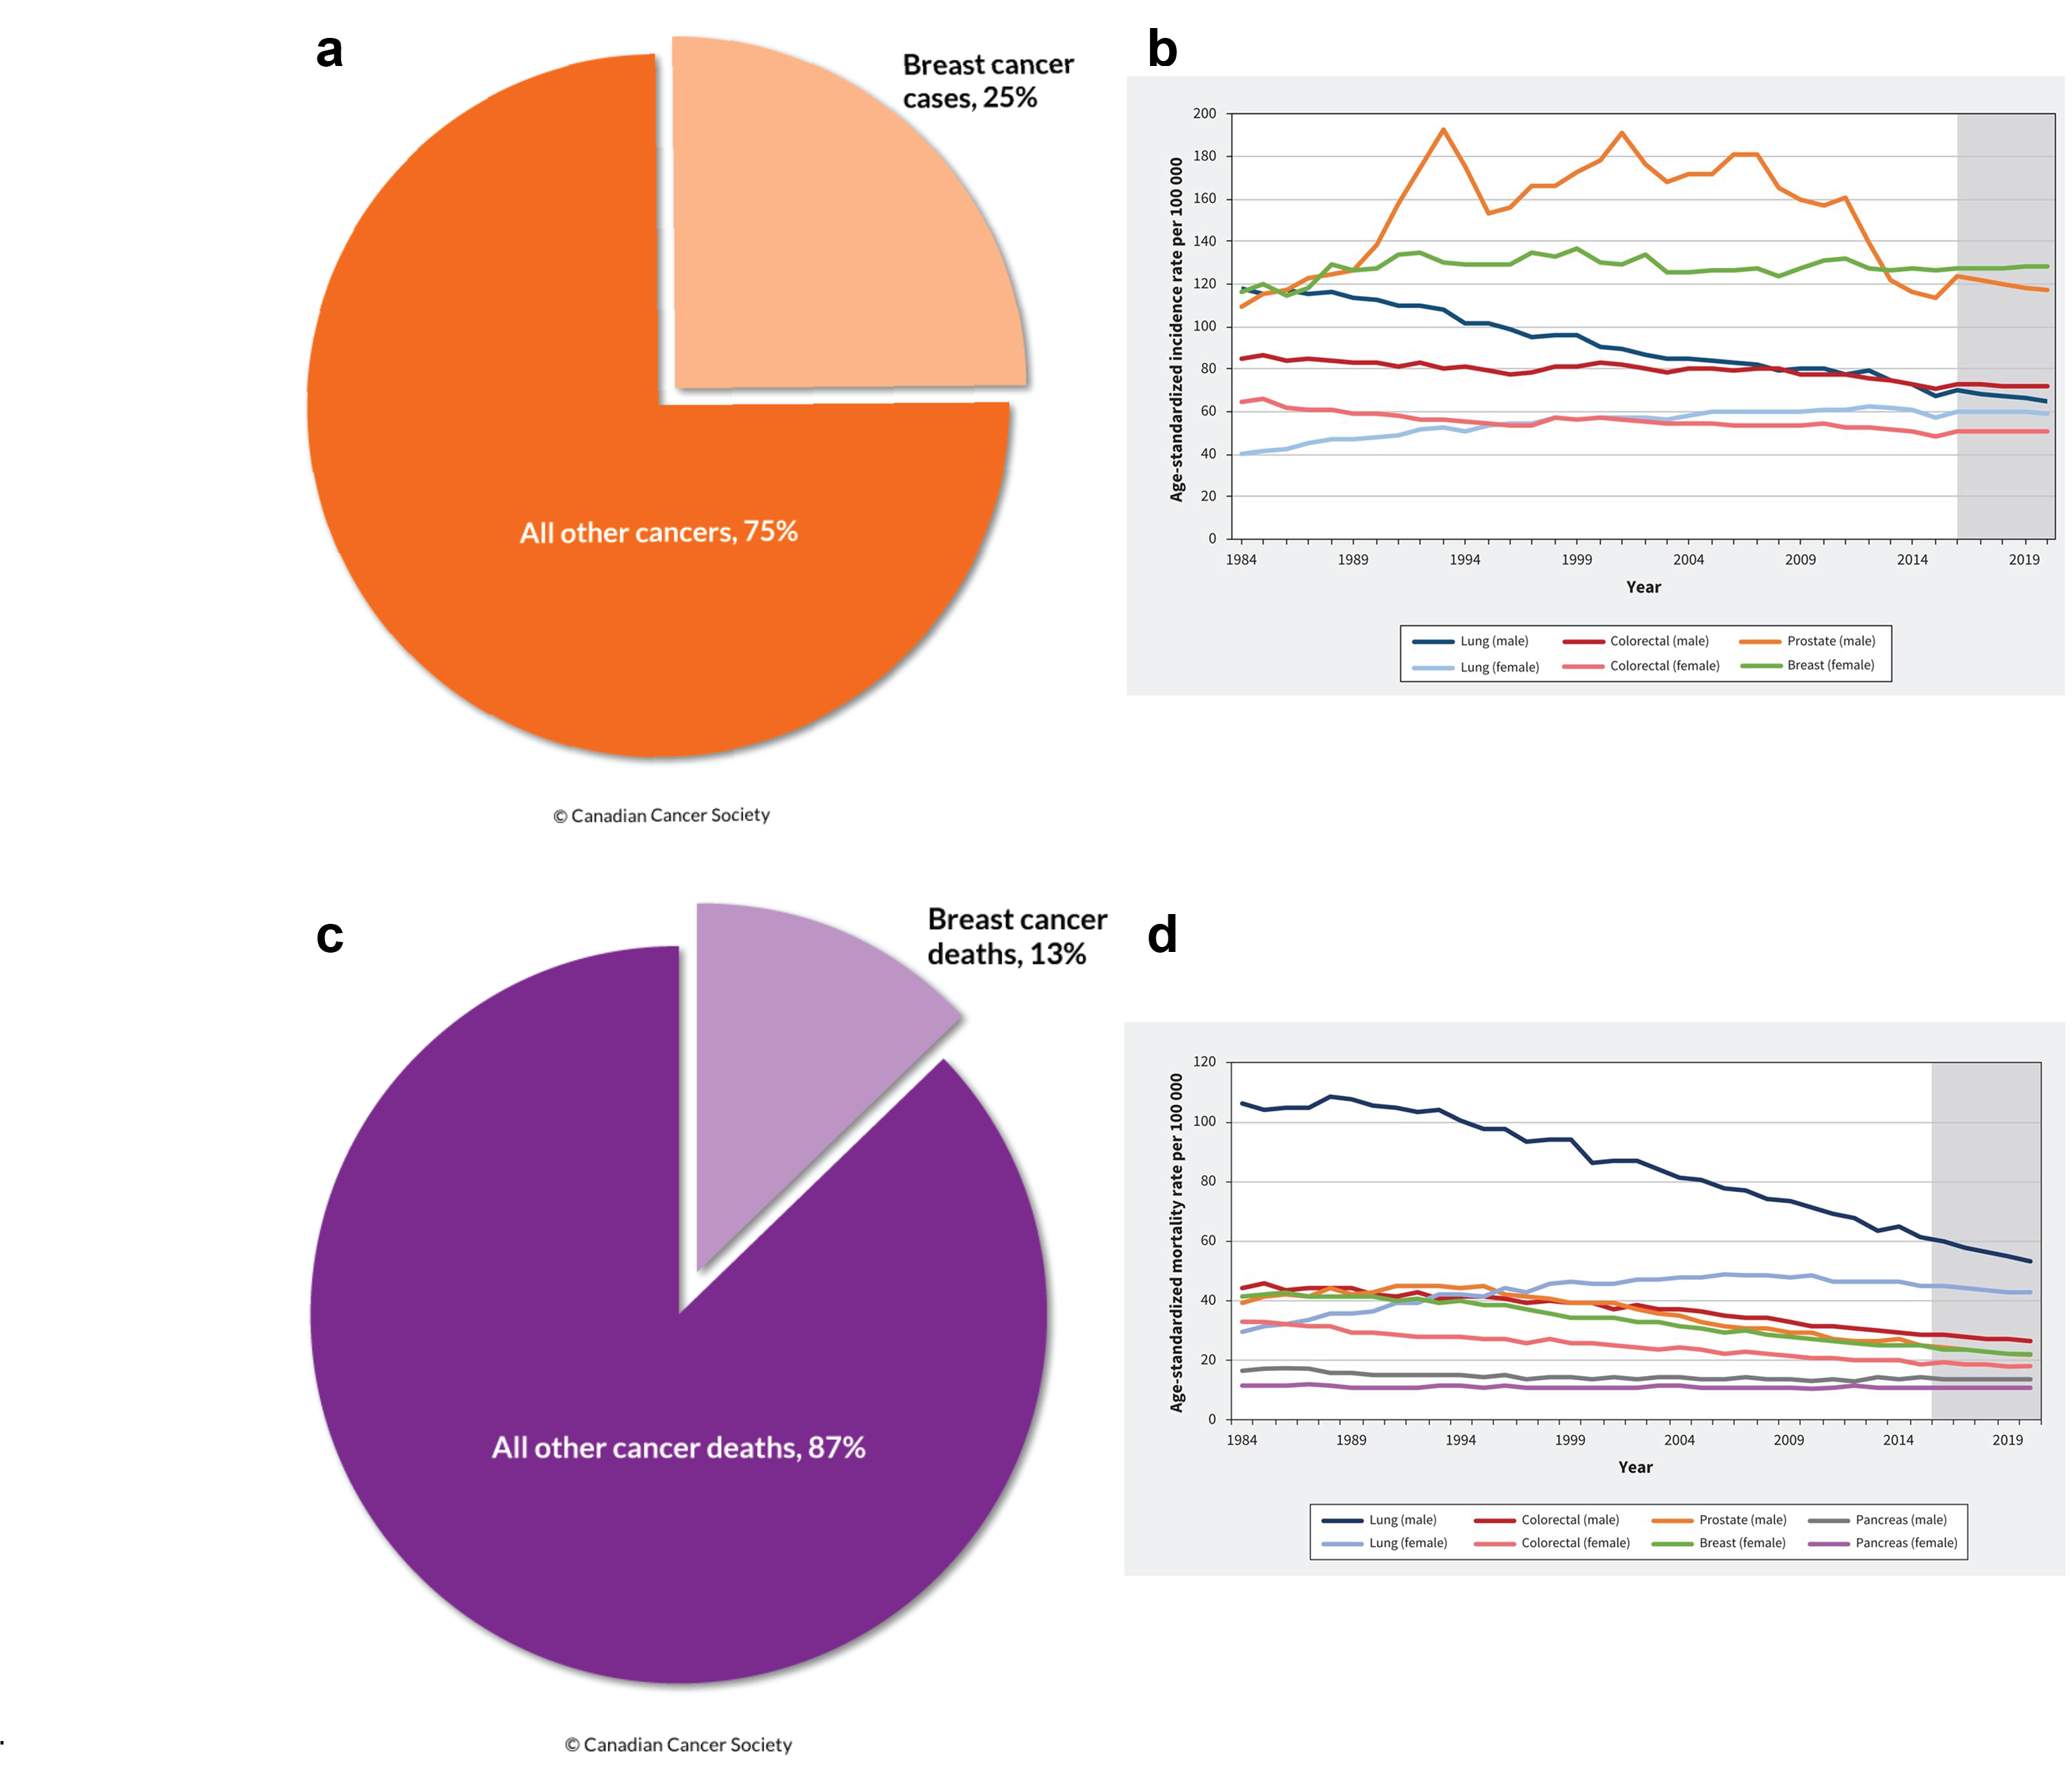
\includegraphics[width=\textwidth]{Figures/chap1/breastcancerstats.png}
	\caption[Breast cancer statistics by Canadian cancer society ]
	{\small
	    \textbf{Breast cancer statistics by Canadian Cancer Society.}
	    \textbf{(a)} Percentage of all estimated new cancer cases in women in 2020.
	    \textbf{(b)} Age-standardized incidence rates (ASIRs) for selected cancers, in Canada (excluding Quebec), 1984 to2020, by sex. Shading indicates projected data.
	    \textbf{(c)} Percentage of all estimated cancer deaths in women in 2020
	     \textbf{(d)} Age-standardized mortality rates (ASMRs) for selected cancers in Canada, 1984 to 2020, by sex. Shading indicates projected data.
	}
	\label{fig:breastcancerstats}
\end{figure}

%%%%%%%%%%%%%%%%%%%%%%%%%%%%%%%%%%%%%%%%%%%%%%%%%%%%%%%%%%%%%%%%%%%%%%

\section{Breast cancer heterogeneity}
 Tumours that originate from different tissues and cells diversify in terms of their genomic as well as transcriptomic landscapes.
 However, genomic aberrations, phenotypic characteristics, such as, stromal recruitment, metastasis, evolution of drug resistance, and drug sensitivity vary between tumours that originate from the same tissue and cell type \cite{vogelstein2013cancer}. 
Tumour heterogeneity thus makes every cancer a unique disease. Heterogeneity occurs, between patients, and within patients over time and space. 
The presence of distinct subpopulations of cells within a tumour, with distinguishable genotypic and phenotypic differences, was classically demonstrated several decades ago \cite{fidler1978tumor}.
The concept of intratumour heterogeneity implies to the presence of distinct tumour cell populations (with different molecular and phenotypical profiles) within an individual tumour following variability over time during tumour growth \cite{ellsworth2017molecular, welch2016tumor}. Inter and intratumour heterogeneity have significant implications for the choice of chemotherapy to govern clinical decision-making in cancer medicine \cite{bedard2013tumour}.



\subsection{Breast cancer subtypes}
To date, several studies have shown that the breast cancer subtypes are associated with variations in treatment response and disease-specific outcomes \cite{metzger2013patterns, arvold2011age}. 
They are identified based on their histological and molecular subtypes. 
Around 50\% to 80\% of newly diagnosed breast cancer cases are
invasive ductal carcinoma (IDC) subtype, while invasive lobular carcinoma (ILC) cases make up less than 10\%. \cite{henry2019breast}.
Based on  gene expression profile studies, four clinically relevant molecular subtypes include; \textbf{Luminal A} (ER+, PR+, HER2-, Ki67low), \textbf{Luminal B} (ER+, PR-, HER2-, Ki67high or ER+, PR-/+, HER2+, Ki67low/high), \textbf{HER2+} (ER-, PR-, HER2+, Ki67high) and \textbf{Triple Negative} (ER-, PR-, HER2-, Ki67high \cite{nadia2017gm, do2020histological}.

The estrogen receptor (ER), progesterone receptor (PR), and ERBB2 also known as human epidermal growth factor receptor 2 (HER2) is routinely determined in all invasive breast carcinomas by immunohistochemistry (IHC) as recommended by cancer control committees and unions \cite{turashvili2017tumor, hammond2010college, wolff2013american}. These are categorized as subtypes of breast cancer and are characterized by their molecular profiles, morphology, and expression of specific biomarkers. The receptor status in the growing tumours also creates another complex layer of intra tumour heterogeneity. For example, some cells that express ER in breast tumours varies from 1 to 100\% cells in the tumour \cite{januvskevivciene2019heterogeneity, visvader2011cells}. These receptors are actionable targets for treatments such as hormone therapies with drugs like tamoxifen, a non-steroidal antiestrogen, used to treat estrogen receptor positive breast cancers \cite{jordan2003tamoxifen,fisher2005tamoxifen} and monoclonal antibodies, such as, herceptin that targets overexpressed ERBB2 (HER2), proven to be effective \cite{piccart2005trastuzumab,slamon2011adjuvant}.  
For the scope of this thesis, I have worked with three triple negative breast cancers (Chapter 4, 5) and one HER2+ (Chapter 4) breast cancer.

%------------------------------------------------------------
\begin{figure}
\centering
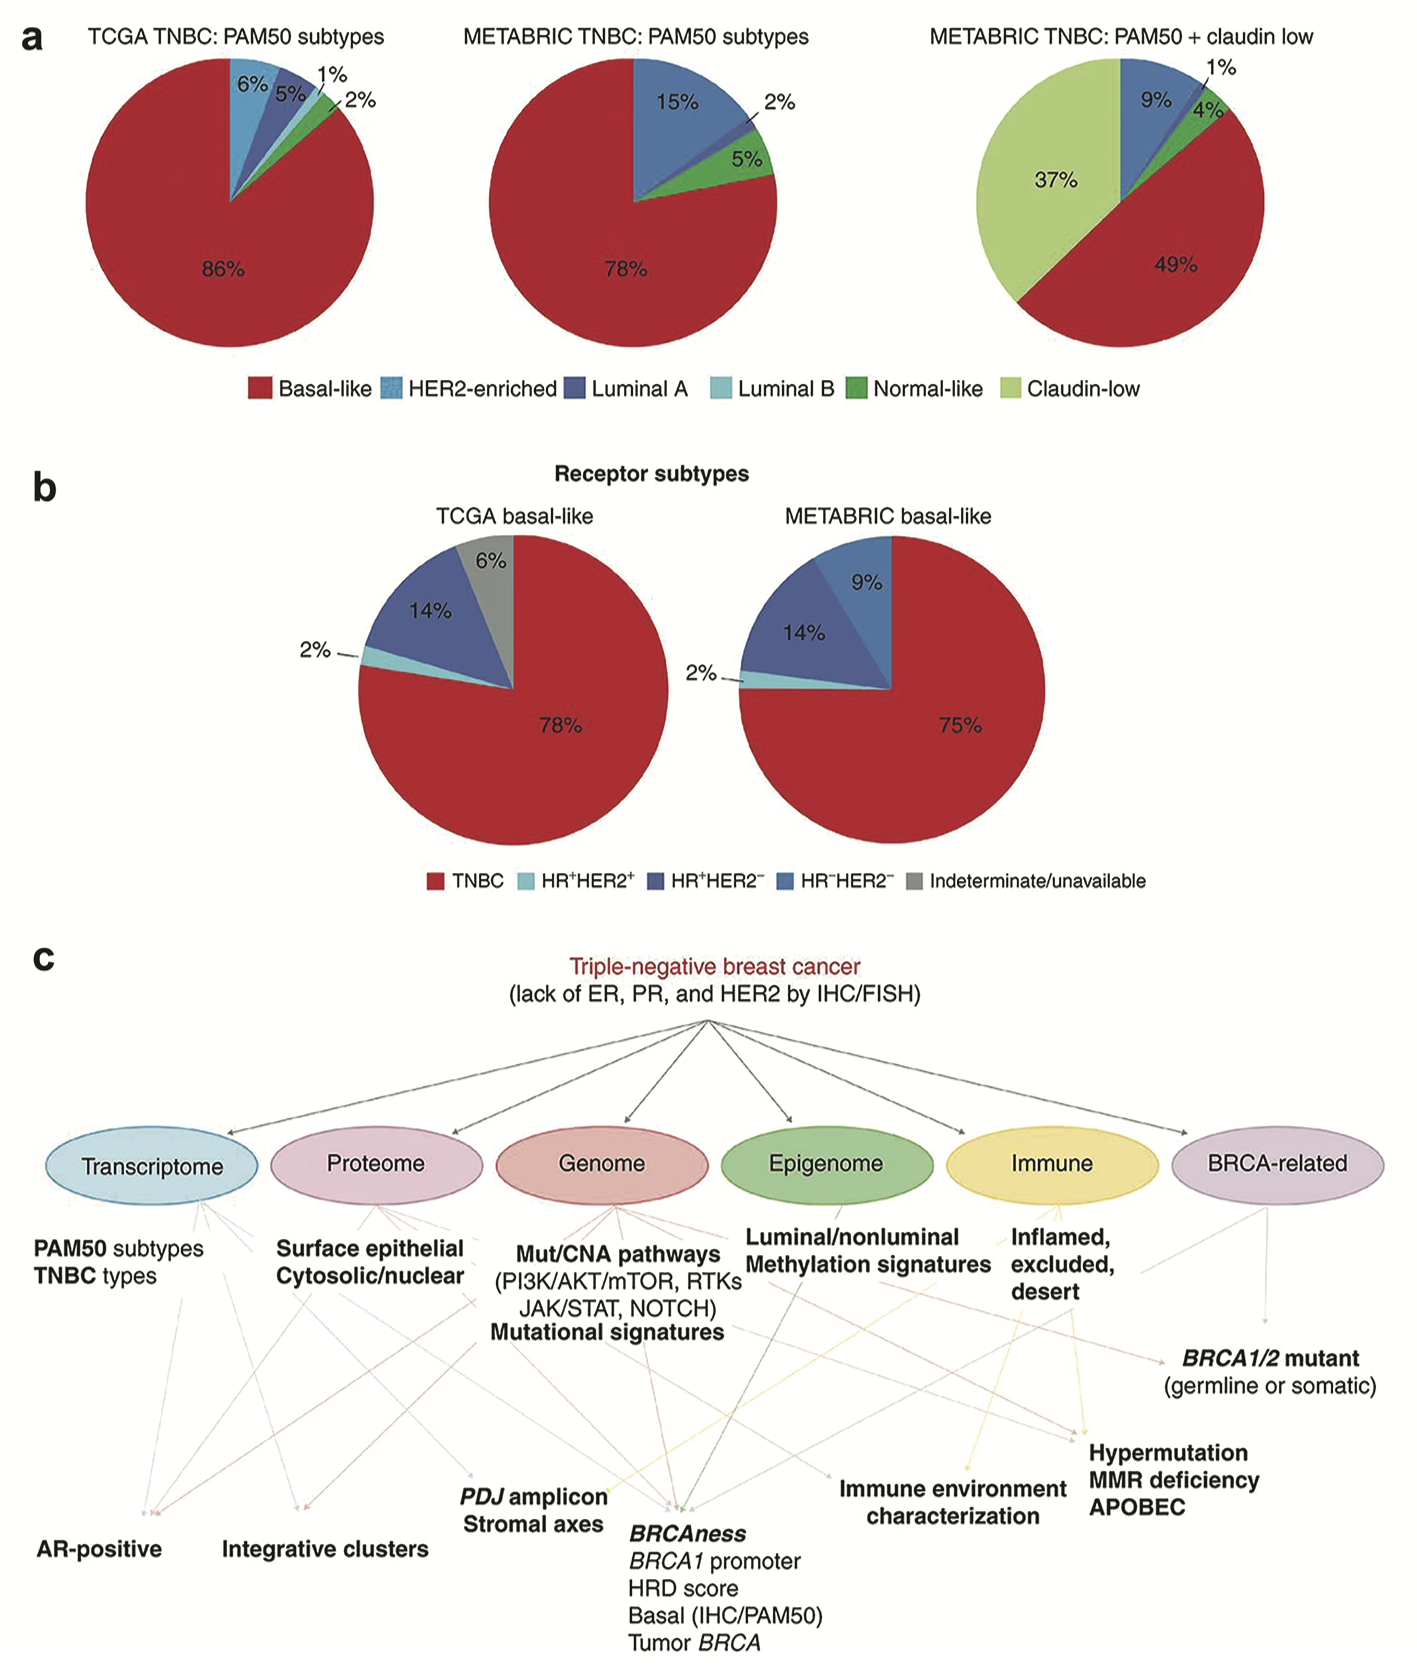
\includegraphics[width=\textwidth]{Figures/chap1/Breastcancersubtypes.png}
	\caption[Breast cancer subtypes]
	{\small
	    \textbf{Breast cancer TNBC intrinsic subtypes adapted from \cite{garrido2019insights}.}
	    \textbf{(a)} Intrinsic subtypes defined by PAM50 and PAM50 + claudin-low in The Cancer Genome Atlas (TCGA) and METABRIC data sets in \ac{TNBC}.
	    \textbf{(b)} Distribution of breast cancer subtype according to receptor status defined by IHC in TCGA and METABRIC data sets in basal-like breast cancer.
	    \textbf{(c)} Interactions among molecular classifications of TNBC based on genomic, transcriptomic, proteomic, epigenomic, and immune characterization of the tumour and its microenvironment. ER, estrogen receptor; PR, progesterone receptor; RTK, receptor tyrosine kinase; MMR, mismatch repair; CNA, copy-number alteration; AR, androgen receptor; HRD, homologous recombination deficiency; IHC, immunohistochemistry; PDJ (PD-L1/2, JAK2).
	}
	\label{fig:Breastcancersubtypes}
\end{figure}
%---------------------------------------------------------------



\begin{figure}
\centering
\includegraphics[width=\textwidth]{Figures/chap1/TNBChistologicsubtypes.png}
	\caption[TNBC histologic subtypes adapted from  \cite{bianchini2016triple} ]
	{\small
	    \textbf{TNBC histologic subtypes adapted from \cite{bianchini2016triple}.}
	    \textbf{(a)}, Histological subtypes. Some rare but relevant subtypes are shown for
illustrative purposes.
	    \textbf{(b)}, Gene-expression-based subtypes of triple-negative breast cancer (TNBC) according to PAM50 \cite{prat2013molecular}.
	    \textbf{(c)}, Gene-expression-based subtypes defined by Lehmann \textit{et al.} \cite{lehmann2011identification}
	     \textbf{(d)} Integrative clusters (IntClust) of genomic and transcriptomic data applied to basal-like breast cancer (BLBC) defined by gene-expression.
	     \textbf{(e)} Heterogeneity of tumour infiltrating lymphocytes. Tumours with low, intermediate and high lymphocyte infiltration are shown for illustrative
purposes. BL1, basal-like 1; BL2, basal-like 2; IM, immunomodulatory; LAR, luminal androgen receptor; M, mesenchymal;
MSL, mesenchymal stem-like; UNC, unclassified; UNS, unstable.
	}
	\label{fig:TNBChistologicsubtypes}
\end{figure}
%------------------------------------------------------------
\subsection{Insights into triple negative breast cancer subtypes heterogeneity}
Patient grouping defined by the absence of biomarkers ER, PR and HER2 are usually referred to as ``triple-negative breast cancers (TNBC)''. It constitutes an extremely heterogeneous group in regards to histology, genetic diversity and treatment resulting in poor prognosis. TNBC accounts closer to $\sim$~15\% in large population series of newly diagnosed breast cancers \cite{reis2008triple}.
The overall survival rate of TNBC is shorter as compared to other breast cancer subtypes and the mortality rate within the first 5 years after diagnosis is 40\%. The recurrance rate in TNBC after surgery is  around 25\% with distant metastasis developing in three years of diagnosis. Unfortunately, the median survival rate, after metastasis, is only 13.5 months \cite{dent2007triple,lin2008sites}. These incidence rates signify the need to understand the extent and mechanisms of heterogeneity in TNBC, which effects treatment outcome. 

Triple negative breast cancers have been redefined over the last decade by METABRIC consortium \cite{curtis2012genomic, dvinge2013shaping, pereira2016somatic, dawson2013new, bilal2013improving}, TCGA \cite{weinstein2013cancer}, ICGC breast \cite{international2010international} and Broad \cite{banerji2012sequence, rheinbay2017recurrent} into two major molecular sub groups (\textbf{\autoref{fig:Breastcancersubtypes} a, b}) \cite{xu2014omics}.

The first group constitutes approximately 75\% of genomically unstable sub-type, with high levels of \ac{CNA}, Loss of heterozygosity (LOH) and structural variations accompanied by basal expression pattern, ubiquitous p53-mutation and high clonal complexity \cite{shah2012clonal, garrido2019insights}. These patients have poor prognosis. The remaining around 25\%, non-basal PIK3CA-enriched TNBC, form distinct groups and have generally better prognosis. Androgen receptor (AR) expressing subset is another known subtype category of TNBC \cite{tang2012expression, rakha2007prognostic,mrklic2013expression}. There is an increasing interest in the possible efficacy of antiandrogen therapies in TNBC \cite{gerratana2018androgen,gucalp2013phase}.
All these subtypes have complex interaction between them summarized in \textbf{\autoref{fig:Breastcancersubtypes} c}.


Extensive research has focused on identifying practical subtypes of TNBC bearing uniformly actionable molecular features. They are described based on their histological and molecular classifications in \textbf{\autoref{fig:TNBChistologicsubtypes}} \cite{weigelt2009histological,bianchini2016triple}. 

\subsection{Relationship of genomic instability and heterogeneity in TNBC}
Genomic instability (GI) refers to the increased tendency to give rise to genomic alterations. It drives heterogeneity and is a hallmark of cancer and results in inter and intratumour heterogeneity \cite{hanahan2011hallmarks}.
 Cells that have intrinsic genomic instability are predisposed to increased mutation rates resulting in evolution of tumour subpopulations with remarkably distinct phenotypes such as metastatic potential and therapeutic resistance \cite{fidler1978tumor, burrell2013causes,januvskevivciene2019heterogeneity}.
TNBC show distinct patterns of copy number based genomic alterations and defects in homologous recombination (HR).
In contrast to estrogen receptor positive breast cancer, where there is a clear gain of 1q and 16p and loss of 16q and HER2 positive subtype, that shows focal high-level amplifications, TNBCs are characterized by a network of low amplitude gains and losses over short chromosome segments with many copy number transitions \cite{kwei2010genomic}.
As compared to other subtypes, TNBCs also present high levels of chromosome instability with loss or gain of larger chromosome fragments or the entire chromosome causing significant structural variation and heterogeneity \cite{lee2016mechanisms}.
The elevated genomic instability creates a complex heterogeneous tumour composed of multiple sub-clones that could progress generating clones having selective advantage conferring drug resistance. 

Genomic instability occurs through various mechanisms, including DNA damage checkpoints, the DNA repair network and the cell cycle checkpoints. BRCA-mutated TNBC are defective in homologous recombination (HR) with advanced and higher tumour grades, distinct metastasis and frequent BRCA1 mutations of $\sim$ 60\%, however, no specific association is observed for BRCA2 mutation carriers \cite{boyle2012triple, atchley2008clinical}. These mechanisms are either operated during tumour development, or influenced by external pressure including exposure to chemotherapies \cite{burrell2013causes,ding2012clonal,hunter2006hypermutation}.

These patterns of genomic instability leave distinct genetic footprints causing cancer evolution inturn affecting therapeutic outcome. 

%%%%%%%%%%%%%%%%%%%%%%%%%%%%%%%%%%%%%%%%%%%%%%%%%%%%%%%%%%%%%%%%%%%%%%

\section{Chemotherapeutic strategies in TNBC}
Due to the lack of distinct endocrine therapies and target candidates in TNBC, more traditional chemotherapy methods are employed to treat TNBC. For more than a decade, a large amount of literature has shown a significantly higher remmission rate in TNBC by using neo-adjuvant chemotherapy (NAC) \cite{liedtke2008response,symmans2017long}. Neoadjuvant chemotherapy refers to the drugs that are administered before surgery. It has been shown previously that the \ac{pCR} of platinum based alone or in combination with paclitaxel, epirubucin or doxorubicin as a neoadjuvant therapy, is between 22\% and 65\%,  
more favourable in TNBC \cite{silver2010efficacy,petrelli2014value,garber2006neo,frasci2009preoperative}. There still are many ongoing clinical trials on neoadjuvant chemotherapies selection in TNBC (including some PARP inhibitors in BRCA deficient tumours), and are reviewed in detail by Tufanno \textit{et al}. in an update article \cite{tufano2020updates}.

The adjuvant therapies are given after initial intervention, usually surgery, to achieve maximum effectiveness. The choice of adjuvant chemotherapy should be individualized based on a number of factors, including tumour stage and grade, rate of disease progression and previous chemotherapy exposure \cite{cardoso20173rd,partridge2014chemotherapy}. According to the national comprehensive cancer network guidelines, TNBCs are treated with a combination of platinum based compounds (DNA-damaging agents), taxanes (microtubule stabilizers-mitotic inhibitors), anthracyclines (DNA intercalators), cyclophosphamide (alkylating agents) and Fluorouracil (antimetabolites) \cite{daly2020nccn}.


Furthermore, most cases of TNBC have unstable genomes complicated with copy number variations, SNVs and structural rearrangements. This high degree of genomic instability can create a very heterogeneous tumour composed of multiple sub-clones which could aid in generating clones that have a selective advantage conferring drug resistance. Drug resistance, whether inherited or acquired, results in challenges to treatment and a worse outcome for the patient.

In Chapters 4 and 5, Cisplatin is selected to perturb tumours to decode clonal and evolutionary dynamics, at genomic and transcriptomic levels, respectively. To compare and contrast cisplatin induced dynamics, CX5461 (G4-quadruplex) was applied in one of the three TNBC PDX. Here we will give an overview of these two drugs.

%...............................................................

\subsection{Cisplatin}
Cis-diamine-dichloroplatinum (II) (also known as cisplatin or CDDP),  is a largely employed platinum compound that causes DNA damage in  a wide spectrum of solid cancers.  At present, around 22 clinical trials are probing the use of cisplatin to treat TNBC either as a single agent or in combination with other therapies \cite{us2017clinicaltrials}.
There is a renewed interest in treating TNBC with cisplatin.
In particular, use of cisplatin therapy has been suggested for TNBC harboring a BRCA mutation \cite{caparica2019treat,petrelli2016platinum}. 
% why there is 
%...................................................................

\subsubsection{Mechanism of action}
Cisplatin is a DNA-intercalating agent \cite{dasari2014cisplatin, kartalou2001mechanisms}. Copper transporter proteins (CTR1 and CTR2) are involved in the uptake of the cisplatin by facilitated diffusion in an inactive form \cite{arnesano2018platinum,ishida2002uptake}. Cisplatin gets activated intracellularly by a series of reactions that includes substitution of one or both cis-chloro groups with water molecules \cite{el1999reactions}. This activation takes place because of the different chloride concentration between blood plasma ($\sim${100mM}) and cell cytolasm ($\sim${4mM}) that leads to the generation of highly reactive mono- and bi-aquated cisplatin forms.


%-------------------------------------------------------------------
\begin{figure}
\centering
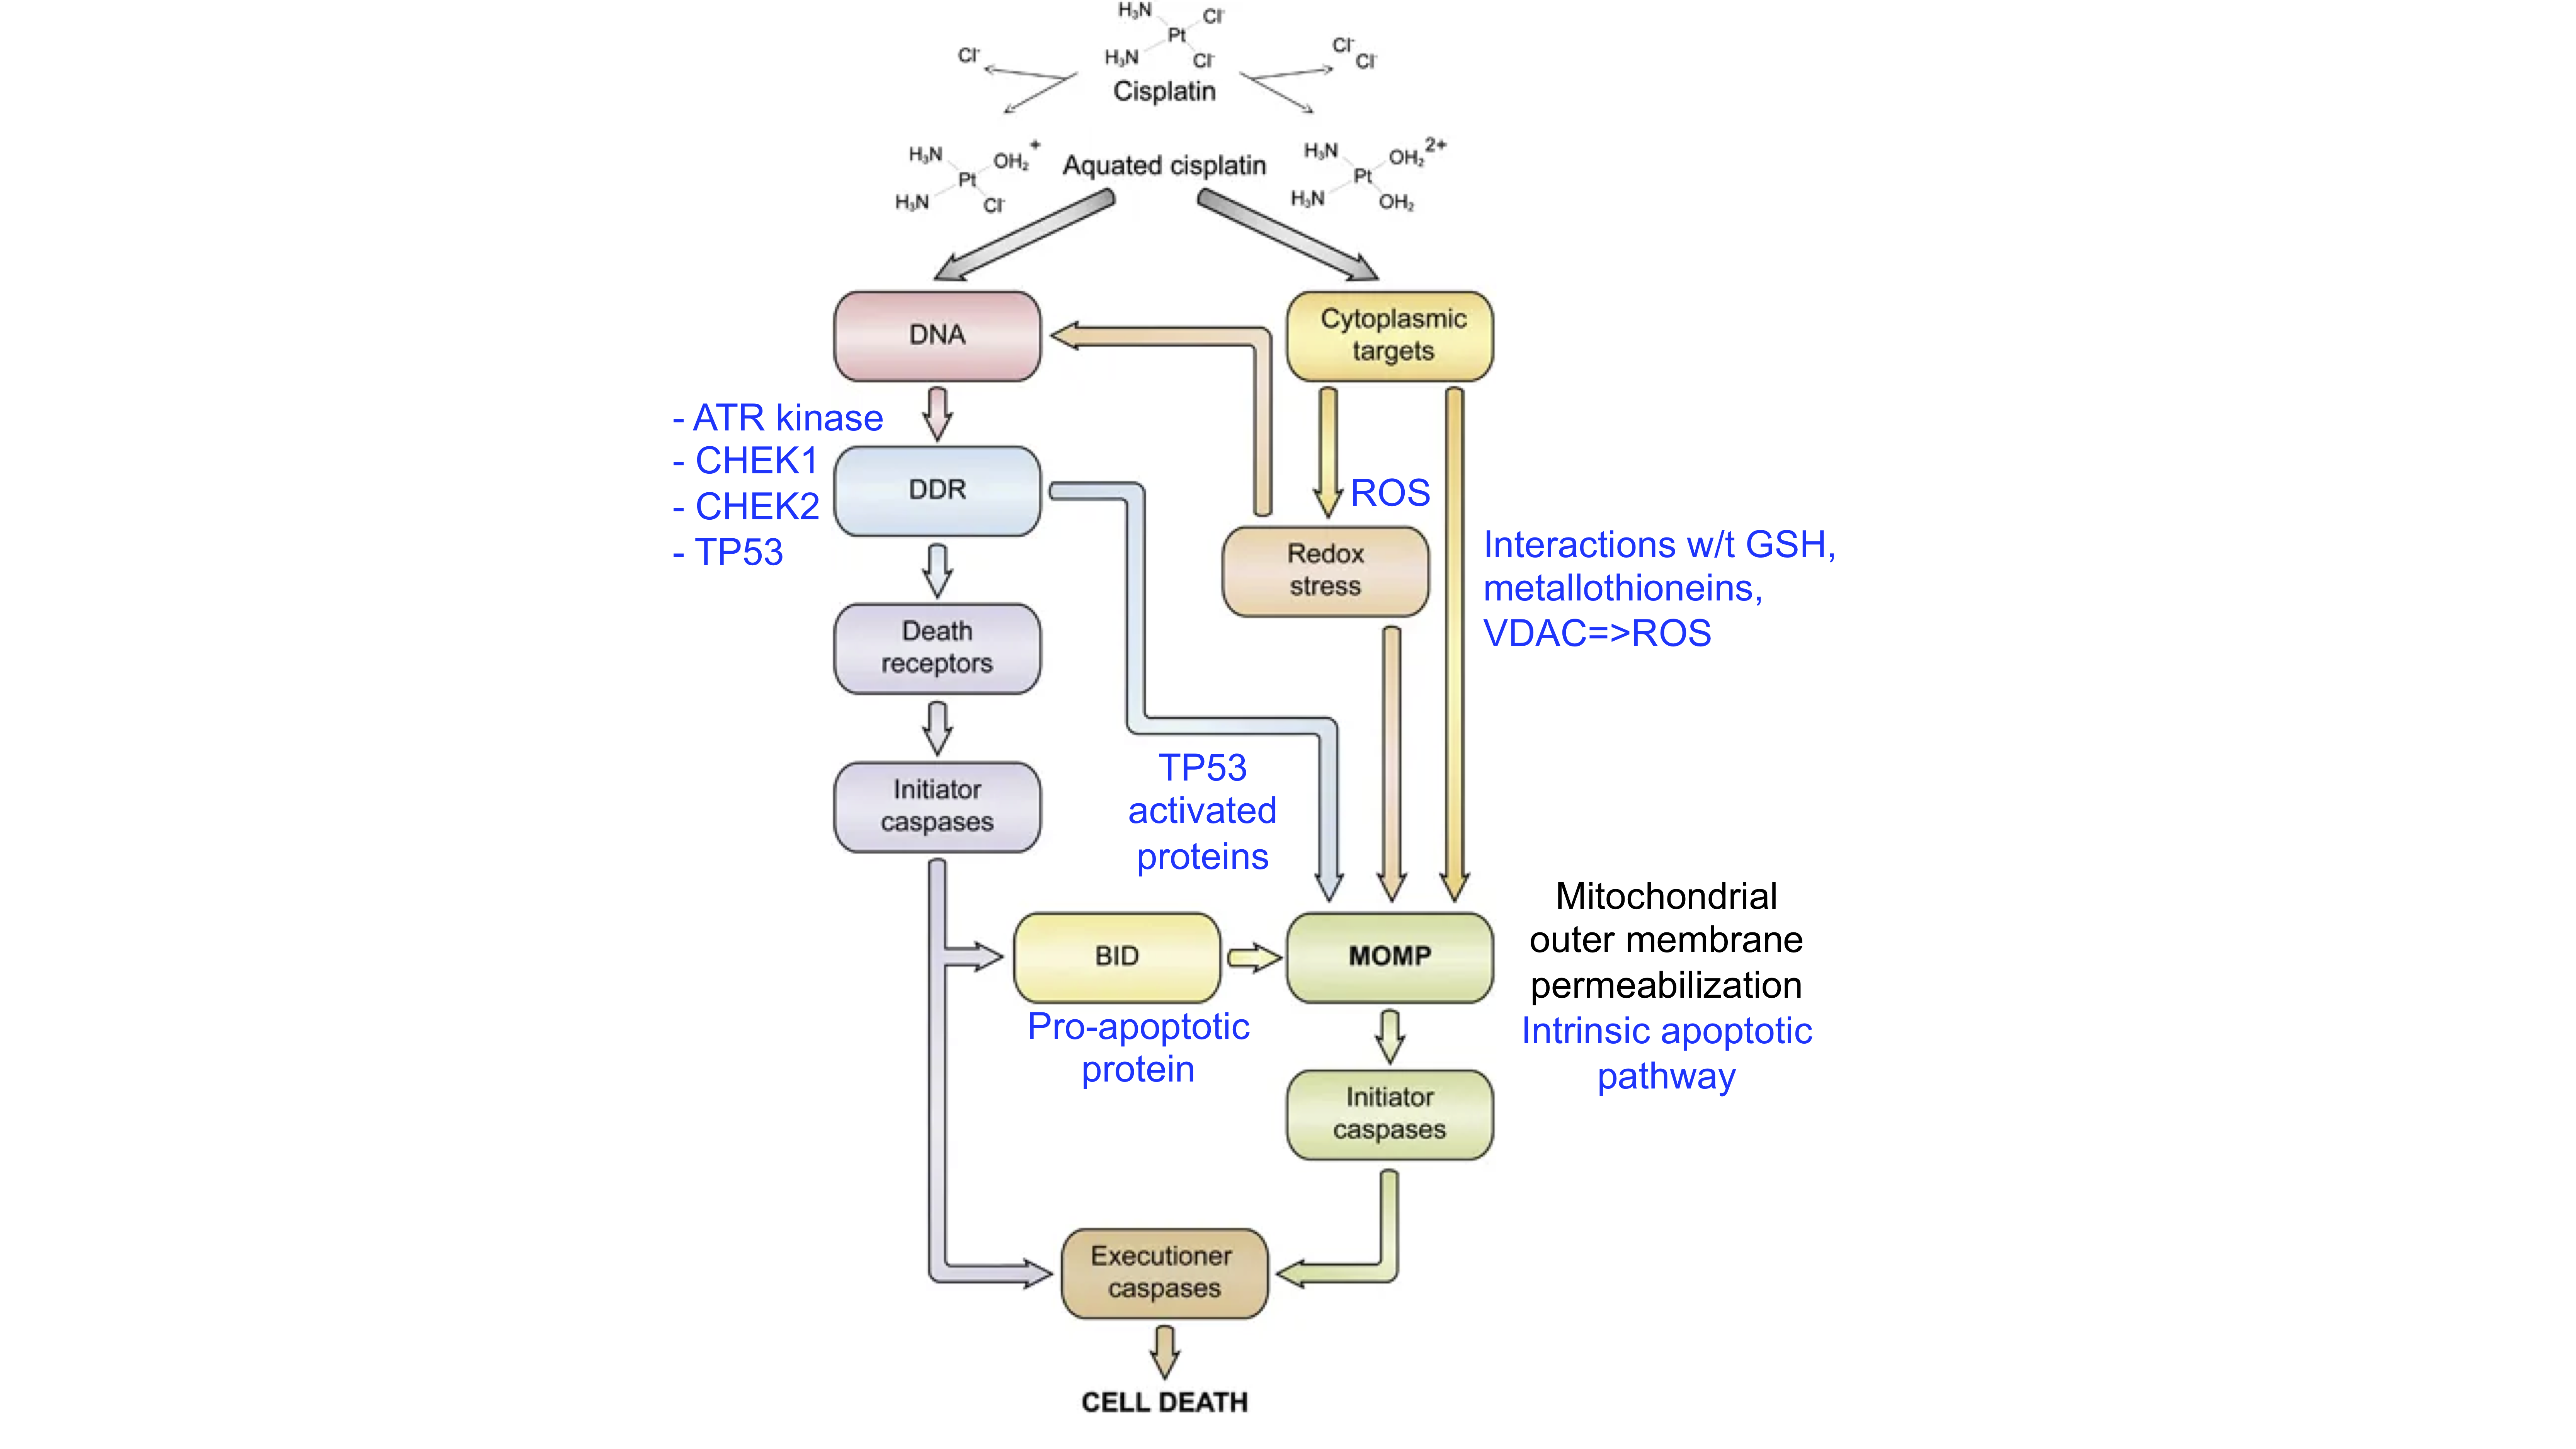
\includegraphics[width=\textwidth]{Figures/chap1/CisplatinMA.png}
	\caption[Mechanism of action of cisplatin]
	{\small
	    \textbf{Mechanism of action of cisplatin modified from \cite{galluzzi2012molecular}}.
	     Intra cellular cisplatin is rapidly aquated due to reduced cytoplasmic concentration of chloride ions. Aquated cisplatin binds to nuclear DNA, thereby promoting DNA damage response. In the cytoplasm, interact with several nucleophiles, including mtDNA as well as multiple mitochondrial and extracellular proteins causing formation of oxidative and reticular stress; provoking a signal transduction cascade that involves pro-apoptotic,BID, BCL-2 family members, as well as VDAC1 and activation of TP53 leading to MOMP and cell death.
	    TP53 activation could directly lead to Cell senescence not shown in the figure. MOMP, mitochondrial outer memberance permeabilization;BID, Bax-like BH3 protein; VDAC, Voltage-dependent anion channel; mtDNA, mitochondrial DNA.
	}
	\label{fig:CisplatinMA}
\end{figure}
%-----------------------------------------------------

The platinum atoms of cisplatin cross-links DNA by making covalent bonds with purine bases in particular with nucleophilic N7 sites. Homotypic intra stand and low percentage of inter strand cross-links result in the generation of DNA-adducts that interfere with DNA replication and RNA transcription. If DNA is not repaired, DNA-damage induced cell-cycle arrest either becomes permanent (an oncosupressive response called senescence) or mitochondrial apoptosis is triggered \cite{fichtinger1985adducts, rabik2007molecular,lopez2013hallmarks}. 

%This effectiveness seems to be due to the unique properties of cisplatin, which enters cells via multiple pathways and forms multiple different DNA-platinum adducts while initiating a cellular self-defense system by activating or silencing a variety of different genes, resulting in genetic and/or epigenetic alterations.
The main signaling cascade that links cisplatin induced DNA lesions to apoptosis involves sequential activation of ATM and RAD3 related protein (ATR, a sensor of DNA damage) and checkpoint kinase 1 (CHEK1, is the downstream effector of ATR) that  eventually phosphorylates the tumour suppressor protein TP53 at serine 20    \textbf{(\autoref{fig:CisplatinMA})} \cite{shieh2000human, cimprich2008atr}. Activated TP53 promotes mitochondrial outer membrane permeabilization (MOMP).  MOMP alone or with stimulatory signals via pro-apoptotic BCL-2 family (BID, BAK1, BAX) \cite {tajeddine2008hierarchical} sets off the caspase dependent cascade and some independent mechanisms that lead to cell death. Checkpoint kinase 2 (CHEK2, is the downstream target of ATM), along with induced cell cycle arrest  (not cell death) through ATM signaling, also responds to cisplatin in an ATM-independent fashion \cite{pabla2008atr}. 

In the cytoplasm, the interaction of cisplatin with glutathione (GSH), metallothionines or mitochondrial proteins for example, voltage-dependent anion channel (VDAC), derives the generation of reactive oxygen species (ROS). ROS and nitric oxide (NO) exacerbate cisplatin toxicity along with increasing the opening of permeability transition pore complex (PTPC) on mitochondria \cite{godoy2012endogenously}. There are also evidence in literature that CHEK1 activates MAPK pathway signaling, mediated by extracellular signal-regulated kinases, c-JUN N-terminal kinases and stress-activated protein \cite{persons2000effect, yeh2002increase}.

\subsubsection{Mechanism of cisplatin resistance}
Cisplatin resistance can arise from transformation in the processes that precede the binding of cisplatin to its actual targets, including cytoplasmic structures and DNA. These factors are categorized as \textbf{pre-target resistance} \textbf{(\autoref{tab:pretargetcisplatinresistance})}. Briefly, copper transporter 1 (CTR1) mediate major fraction of cisplatin intake \cite{more2010role,ishida2010enhancing, holzer2006contribution}, whereas ATPase, copper transporting, beta polypeptide (ATP7B), is involved in cisplatin export \cite{katano2002acquisition,komatsu2000copper, aida2005expression}. Some plasma membrane transporters have been proposed to contribute to the extrusion of cisplatin, including ATP-binding cassette, subfamily C member 2, best known as multidrug  resistance-associated protein 2 (MRP2) \cite {cui1999drug,korita2010multidrug,liedert2003overexpression} and ATP-ase, class VI, type IIB (ATP11B) \cite{moreno2013atp11b}. Moreover, cisplatin resistant cells also exhibit high levels of metallothioneins \cite{kelley1988overexpression,kasahara1991metallothionein} and GSH, an enzyme that catalyzes GSH synthesis (i.e., gamma glutamylcysteine synthetase) and conjugates with cisplatin \cite{lewis1988glutathione,chen2010role}. 

%----------------------------------------------------------------------
\begin{table}[htbp]
   \centering
   \caption{Pre-target cisplatin resistance factors. Modified from \cite{galluzzi2012molecular}}
\begin{tabular}{p{1.5cm}p{5cm}p{5cm}p{1cm}}
\hline
\textbf{Genes/ Factors} & \multicolumn{1}{l}{ \textbf{Mode of Action}} & \multicolumn{1}{p{5cm}}{ \textbf{Importance}} & \multicolumn{1}{p{5cm}}{ \textbf{References}} \\ \hline

CTR1   & Reduced uptake, Plasma membrane copper transporter & Downregulated in resistant cells. CTR1 depletion increases cisplatin resistance. Copper chelators enhance the uptake and efficacy of cisplatin & \multicolumn{1}{p{5cm}}{ \cite{more2010role, ishida2010enhancing,holzer2006contribution,katano2002acquisition}} \\

ATP7A/ ATP7B & Increased efflux, Copper-extruding P-type ATPases involved in the regulation of ion homeostasis & Upregulated in cisplatin-resistant cells. ATP7B expression levels may predict the efficacy of cisplatin chemotherapy.  & \multicolumn{1}{p{5cm}}{\cite{katano2002acquisition,komatsu2000copper,nakayama2002copper,safaei2004role,aida2005expression}} \\ 

MRP2   & Increased efflux, Member of the ABC family of plasma membrane transporters. Mediates the ATP-dependent cellular efflux of cisplatin. & Overexpressed in cisplatin-resistant cells. Modulation by antisense cDNA enhances cisplatin sensitivity. Expression levels affect the efficacy of cisplatin regimens. & \multicolumn{1}{p{5cm}}{\cite{cui1999drug,korita2010multidrug,liedert2003overexpression, yamasaki2011role}} \\

GSH/ GCS/ GST & Increased inactivation, GSH scavenges electrophiles and ROS. GCS catalyzes GSH synthesis. GST conjugates GSH to cisplatin and facilitates its extrusion. & Resistant cells often exhibit high levels of GSH, GCS and GST.  & \multicolumn{1}{p{5cm}}{\cite{lewis1988glutathione,chen2010role}} \\

Metallo-thionein & Increased inactivation, Intracellular thiol-containing proteins involved in the detoxification of metal ions. & May bind and inactivate cisplatin.  & \multicolumn{1}{p{5cm}}{\cite{kelley1988overexpression,kasahara1991metallothionein}} \\   \hline
\end{tabular}%
\begin{tablenotes}
\small
      \item  {CTR1,copper transporter receptor 1; MRP, multi-drug resitance proteins; ROS, reactive oxygen species; GSH, glutathione; GCS,gamma-glutamylcysteine synthetase; GST, glutathione S-transferases}.
    \end{tablenotes}
 
   \label{tab:pretargetcisplatinresistance}%
 \end{table}%
%-----------------------------------------------------------------------

The mechanism of \textbf{on-target cisplatin resistance} is believed to arise in particular with the removal of cisplatin DNA-adducts and subsequent apoptosis can be defective in cisplatin-resistant cancer cells due to a variety of mechanisms including nucleotide excision repair (NER) proficiency \cite{wood2000dna, shuck2008eukaryotic}. They are summarized in \textbf{\autoref{tab:ontarget}}. In addition, another proposed mechanism for cisplatin resistance involves high expression of the high-mobility group box protein 1 (HMGB1), that appears to bind selectively to cisplatin DNA crosslinks and interferes with \ac{NER} while HMGB3 is associated with the promoter regions of ATR and CHK1 \cite{awuah2017repair, mukherjee2019targeting}. 


%------------------------------------------------------------

\begin{table}[htbp]
   \centering
   \caption{On-target cisplatin resistance factors. Modified from \cite{galluzzi2012molecular}}
    \begin{tabular}{p{1.5cm}p{5cm}p{5cm}p{1cm}}
     \hline
      \textbf{Genes/ Factors} & \multicolumn{1}{l}{ \textbf{Mode of Action}} & \multicolumn{1}{p{5cm}}{ \textbf{Importance}} & \multicolumn{1}{p{5cm}}{ \textbf{References}} \\ \hline
ERCC1  & Increased NER proficiency, Single-strand endonuclease, in association with ERCC4/XPF incises DNA on the 5' side of cisplatin adducts. & ERCC1 expression negatively correlates with  cisplatin clinical responses in multiple human cancers & \multicolumn{1}{p{5cm}}{\cite{dabholkar1992ercc1, metzger1998ercc1, bellmunt2007gene, shirota2001ercc1}} \\
MLH1 & MMR deficiency, Component of a multiprotein complex that excides and repairs DNA mismatches. Implicated in DNA damage signaling and apoptosis. & MLH1 deficiency is sometimes associated with  cisplatin resistance (and increased TLS).  & \multicolumn{1}{p{5cm}}{\cite{aebi1996loss, gifford2004acquisition}} \\
MSH2  & Forms heterodimers that detect DNA lesions including base-base mismatches. & Low MSH2 levels predict  cisplatin benefits in patients with resected lung cancer. & \multicolumn{1}{p{5cm}}{\cite{kamal2010muts}} \\
POLH & Increased TLS, DNA polymerase that substitutes stalled replicative polymerases and includes nucleotides opposite to the DNA lesion. & POLH upregulation correlates with short patient survival. & \multicolumn{1}{p{5cm}}{\cite{alt2007bypass, shachar2009two}} \\
REV3/ REV7 & Catalytic (REV3) and structural (REV7) subunits of the TLS DNA polymerase . & REV3 defects correlate with increased cisplatin sensitivity in cancer cell lines. REV overexpression is associated with  cisplatin resistance  & \multicolumn{1}{p{5cm}}{\cite{wittschieben2006loss, roos2009translesion}} \\  
BRCA1/ BRCA2 & Increased HR proficiency, HR DNA repair. Regulation of transcription and cell cycle progression. & BRCA1/2-deficient tumours respond better to  cisplatin. Secondary mutations that restore BRCA function favor acquired chemoresistance.& \multicolumn{1}{p{5cm}}{\cite{narod2004brca1, edwards2008resistance, sakai2008secondary}}  \\  
VDAC & Cisplatin binding proteins, protein of the OM that mediates vital functions but also participates into the PTPC.& Depletion/or inhibition of VDAC increases  cisplatin resistance. Might also be involved in post-target resistance.& \multicolumn{1}{p{5cm}} {\cite{yang2006cisplatin,kroemer2010autophagy,tajeddine2008hierarchical}}\\  
    \hline
     \end{tabular}%
  \begin{tablenotes}
      \small
      \item  {ERCC1, excision repair cross-complementing rodent repair deficiency, complement group1, HR, homologous recombination; TLS, translesion synthesis; OM, mitochondrial outer membrane; XPF, xeroderma pigmentosum complementation group; VDAC, voltage dependent anion channel; PTPC, permeability transition pore complex.}
    \end{tablenotes}
 
   \label{tab:ontarget}%
 \end{table}%

%------------------------------------------------------------------------

\begin{figure}
\centering
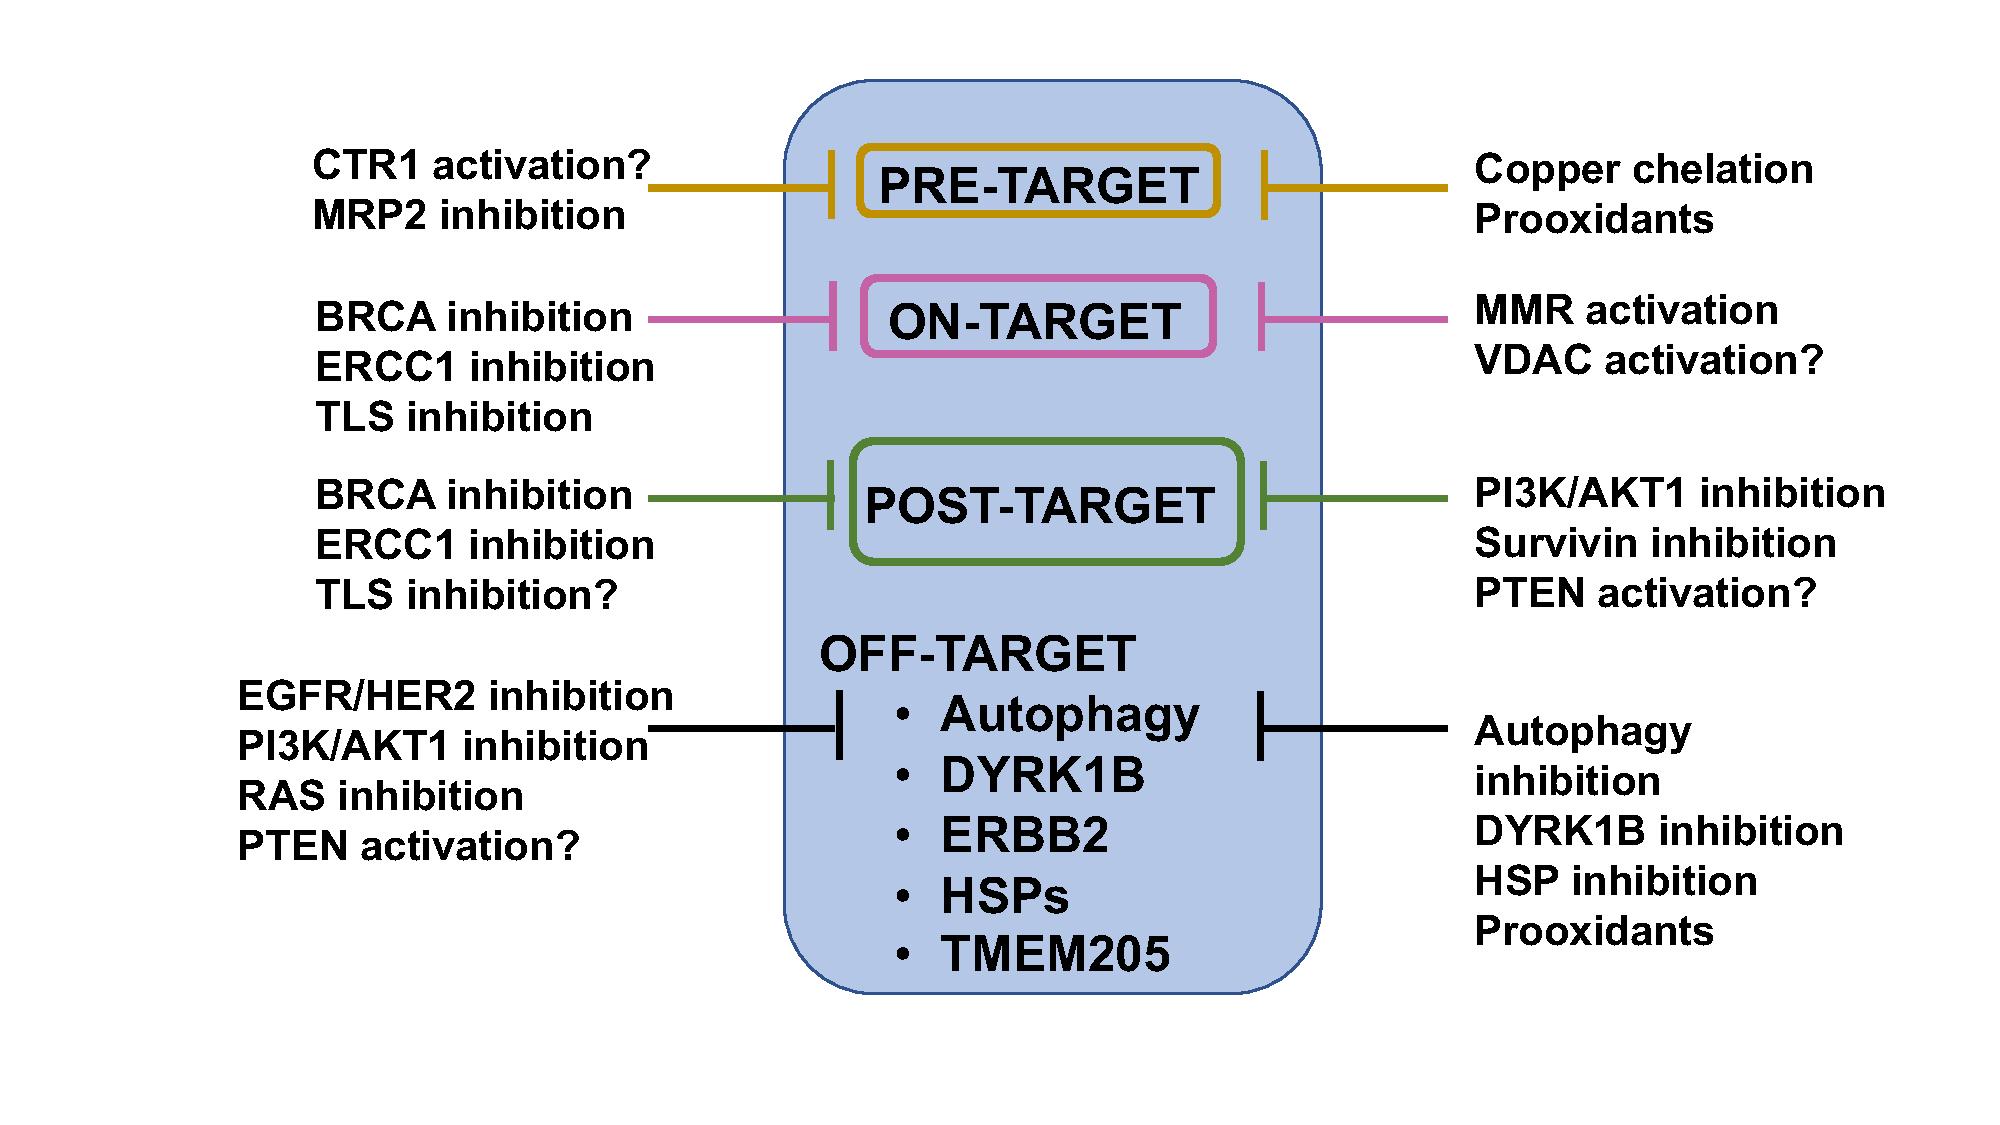
\includegraphics[width=\textwidth]{Figures/chap1/circumventingcisplatinresistance.pdf}
	\caption[Mechanism of action of cisplatin]
	{\small
	    \textbf{Inhibition strategies at various levels of cisplatin resistance mechanisms. Modified from  \cite{galluzzi2012molecular}}.
	     Cisplatin resistance most often has a multifactorial nature, implying that targeting one mechanism of resistance at a time has very low chances to result in significant chemosensitization. Thus, combination strategies for blocking cisplatin resistance at multiple levels should be designed. With regard to this, detailed information on the patient genetic and epigenetic background might be critical for determining which specific mechanisms should be targeted to fully circumvent chemoresistance. CTR, Copper transporter receptor; EGFR, epidermal growth factor receptor; HSP, heat-shock protein; PTEN, phosphatase and tensin homolog; TLS, translesion synthesis.
	}
	\label{fig:circumventingcisplatinresistance}
\end{figure}

%----------------------------------------------------------------------

\textbf{Post-target resistance} to cisplatin can result from alterations in signal transduction pathways that mediate apoptosis in response to DNA damage. Non-repairable cisplatin-induced DNA damage leads to the activation of a multi-branched signaling cascade with proapoptotic outcomes. Several groups have provided evidence that predominant mechanisms involves the inactivation of \textit{Tp53}, which exists in around half of all human cancers \cite{kirsch1998tumor}. Reportedly patients harboring wild-type \textit{Tp53} have a higher probability to take advantage from cisplatin as compared to the patients with \textit{Tp53} mutations \cite{vousden2007p53,gadducci2002molecular}. 
Furthermore, inhibition of PDGFR$\beta$ mediated phosphorylation of AKT by Ly294002 reversed cisplatin resistance \cite{juliachs2014pdgfrbeta}. Somatic mutations within PI3KCA, AKT and FGFR3 were also reported in cisplatin resistance \cite{feldman2014presence}. Pre-clinical studies indicate that targeting PDGFR/PI3K/AKT pathway may reverse cisplatin resistance \cite{juliachs2013effectivity}.
Upregulation of IGF1R expression and signaling was also found to contribute to acquired cisplatin resistance \cite{selfe2018igf1r}. 

Variations in any of the factors that regulate and carry out apoptosis have the potential to influence cisplatin sensitivity. It could be triggered by DNA damage or oxidative stress via the mitochondrial pathway. Numerous proteins including death receptors, cytoplasmic adaptors. pro- and antiapoptotic members of the BCL-2 family, caspases, calpains and many others \cite{jain2011molecular, janson2010resistance, michaud2009bcl}. Ryan \textit{et al.} reported that BIRC5 (Survivin) overexpression is associated with chemoresistance and poor prognosis in multiple types of cancer \cite{ryan2009survivin}. 

Cisplatin-resistant phenotype can also be sustained through \textbf{off-target resistance} including the alterations in signaling pathways that are not directly engaged by cisplatin. Relavant factors include are autophagy, which is evolutionary conserved response to stress conditions including chemotherapy \cite{tan2019trp14}, DYRK1B is a conserved tyrosine kinase that is usually overexpressed in breast cancers and mediates antiapoptotic effects.  \cite{hu2010depleting}, ERBB2 \cite{fijolek2006p53}, HSP (heat shock proteins)  are chaperones that exert prosurvival functions in response to a variety of stress conditions including cisplatin \cite{ren2008down}. 
%and TMEM205 \cite{shen2010elevated}.

In summary, there are at least four distinct but broad categories of mechanisms by which cancer cells become resistant to cisplatin. The major hurdle to overcome this clinically relevant issue is that often more than one resistance mechanism is activated thus exhibiting a multifactorial consequences of cisplatin resistance. It has been speculated that at least two mechanisms should be targeted to restore cisplatin sensitivity, for example, combined interventions that could inhibit pre-target resistance (such as, copper chelators and prooxidants) and/or inhibition of post, on  or off target mechanisms (such as translesion synthesis (TLS) inhibition PI3K/AKT1 inhibition or blockers of autophagy)  \textbf{(\autoref{fig:circumventingcisplatinresistance})} may possibly restore cisplatin sensitivity. It is hard to decide which pathways should be targeted and what combination strategies should be applied to overcome resistance because all mechanisms are not operated at the same time as we observed in chapter 5 while tracking changes in pathways over drug exposure and depends on duration of drug exposure and type of tumour expressing proteins and pathways.

\subsection{CX5461: G4 stabilizer} 
CX5461 is a small molecule G-quadruplex stabilizing compound. It was developed as a selective RNA polymerase I inhibitor \cite{drygin2011targeting}. Recent evidence suggests that it causes DNA damage and induces selective lethality in BRCA1/2 deficient tumours \cite{xu2017cx}, resulting in a first in human Canadian clinical trial (CCTG-IND231). 
 
 \subsubsection{G-quadruplex structures}
G-quadruplex (G4) structures arise transiently at guanine-rich sequences in the folded DNA and RNA, when two or more G-tetrads stack on top of each other and coordinate monovalent cations, such as K+ and Na+ \cite{sen1990sodium} \textbf{(\autoref{fig:G4structures} a)}. Each tetrad is composed of four G residues that are linked by the sugar-phosphate backbone and connected through Hoogsteen-type hydrogen bonds \cite{kwok2017g}. G-quadruplex structures can fold intramolecularly from a single G-rich strand, or intermolecularly through dimerization or tetramerization of separate filaments. They both can present prarallel or anti parallel topologies \textbf{\autoref{fig:G4structures} b}. The length of loop can vary (1-7 nucleotides), with smaller loops being more stable\cite{huppert2010structure}.
G4 sequences mainly clustered in central genomic regions, namely single-stranded 3' overhangs in telomeres, gene promoters, especially oncogenes and DNA replication origins. In cancer cells these structures are important in DNA replication, telomere maintenance, and regulation of transcription and translation \textbf{\autoref{fig:G4structures} c, d, e} \cite{rhodes2015g, maizels2013g4}. Literature based on large scale DNA sequencing on human genome have revealed over 700,000 putative G4 sites and 10,000 of them have been identified from ChIP-seq using an antibody that recognises G4 structures \cite{siddiqui2002direct, granotier2005preferential, chambers2015high, hansel2016g}.

%--------------------------------------------------------------------------
 \begin{figure}
\centering
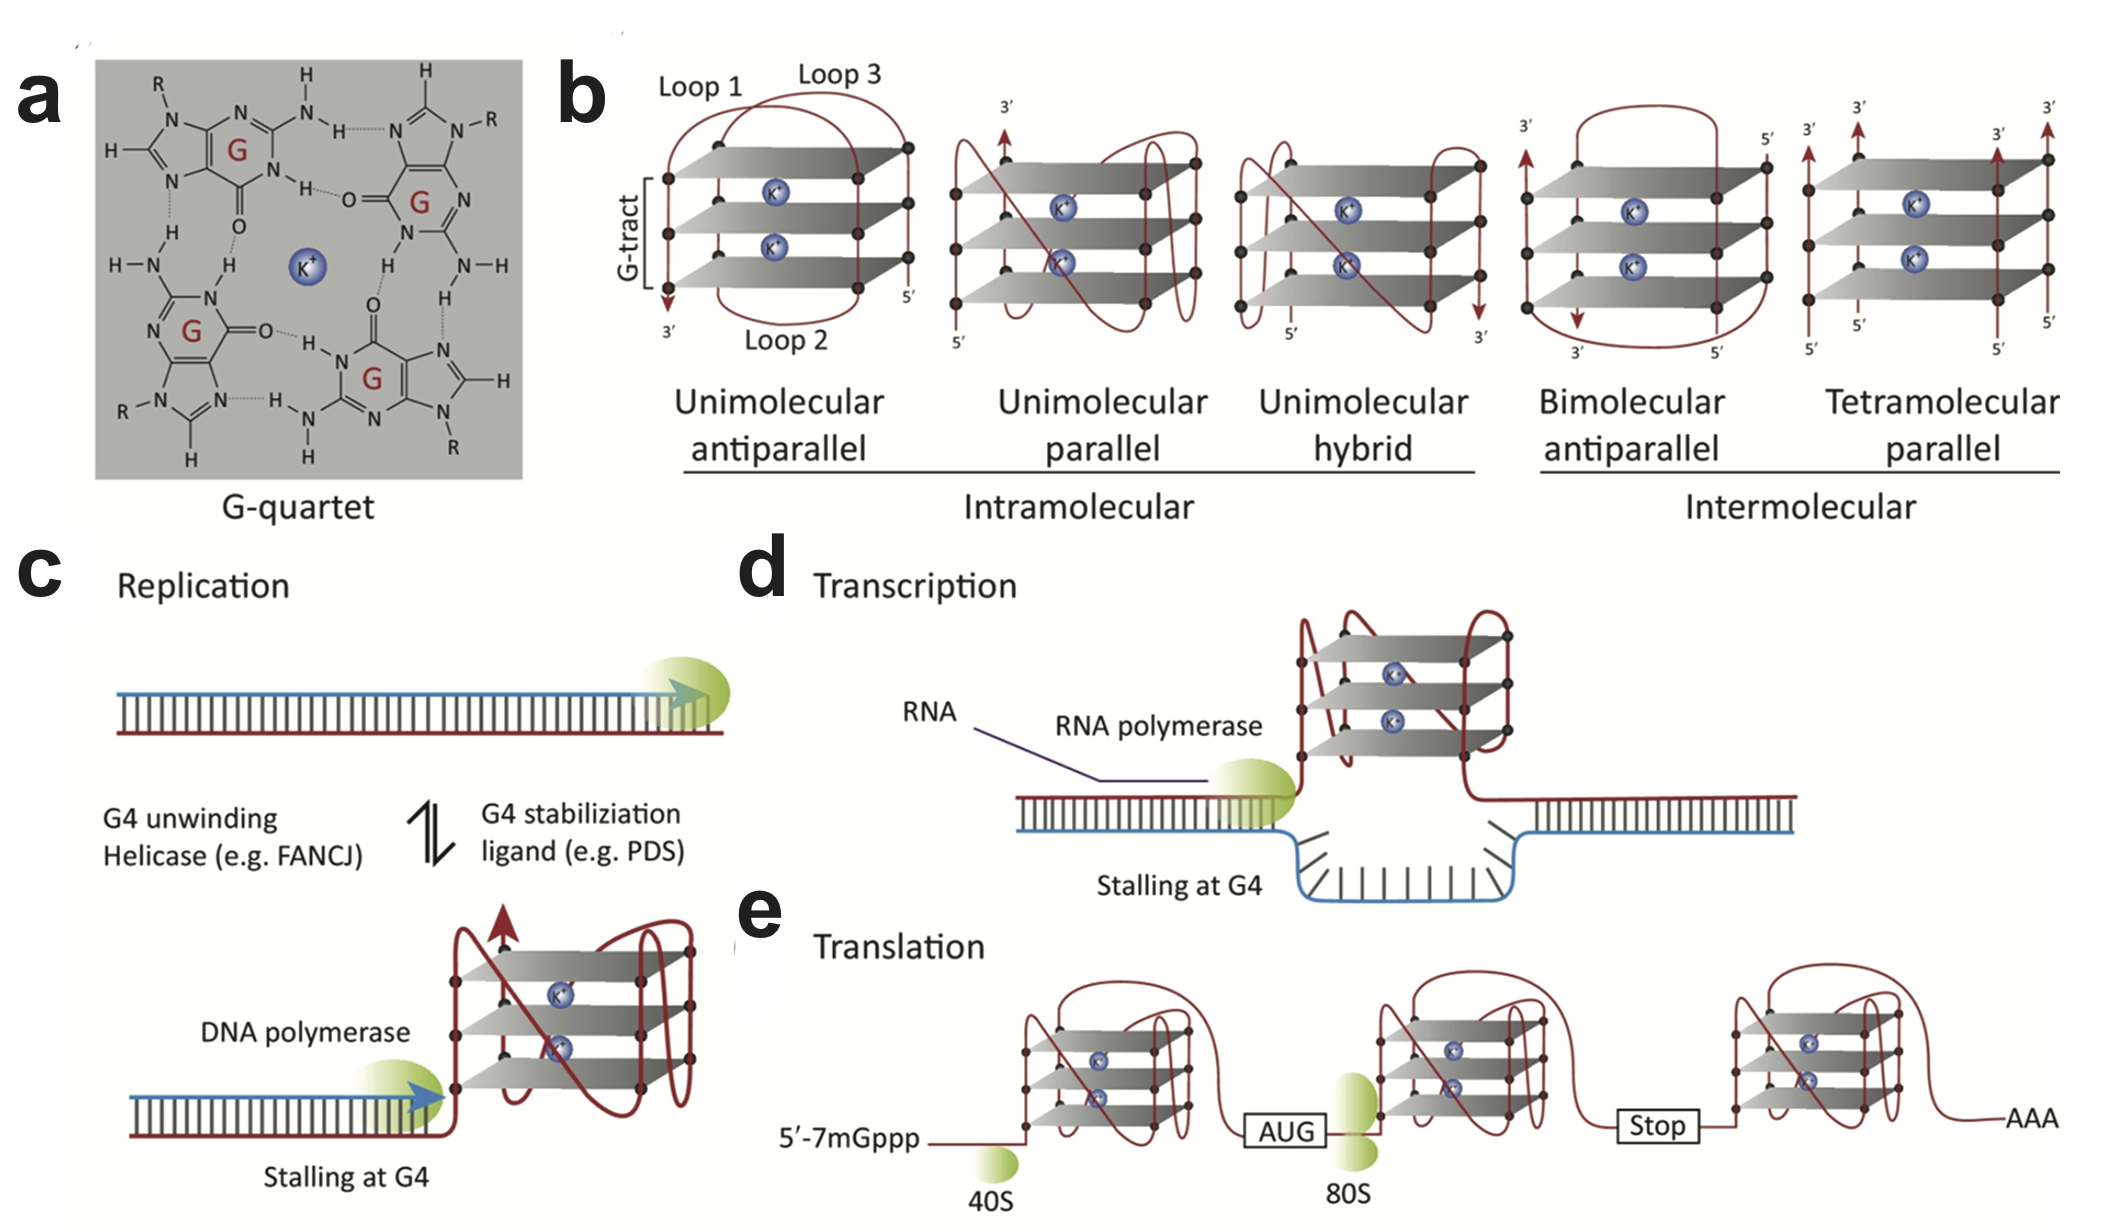
\includegraphics[width=\textwidth]{Figures/chap1/G4structures.png}
	\caption[The G4 structures and their biology]
	{\small
	    \textbf{The G4 structures and Biology. Modified from \cite{kwok2017g}}.
	   \textbf{(a)} Chemical structure of a G-quartet. Potassium ion (K+) sits within the G-quartets for stabilization. G-quartets stack on each other to form G-quadruplex \textbf{(b)} Representative topologies of G-quadruplex structures. \textbf{(c-e)} Representative G-quadruplex-associated biology: regulation of \textbf{(c)} DNA replication, \textbf{(d)} transcription, and \textbf{(e)} translation
	}
	\label{fig:G4structures}
\end{figure}
%------------------------------------------------------------------------------ 
 
 \subsubsection{CX5461 leads to synthetic lethality with  DNA repair pathways deficiency}
 The dominant feature of the p53/basal expression group of TNBC is genomic instability \cite{yu2013identification}. It is important to identify specific subgroups that could be targeted through synthetic lethal approaches, analogous to PARP inhibitors that exploit loss of homologous recombination (HR) repair  \cite{fong2009inhibition}.
 CX5461, in addition to polymerase 1 inhibition and G4 stabilization, has been recently shown to have activity in \ac{HR} and \ac{NHEJ} deficient cancer cells \cite{zimmer2016targeting,xu2017cx}. 
 BRCA1/2 deficiency leads to compromised HR repair, generating an increased error-prone DNA repair and ultimately, genomic instability. The BRCA2/RAD51 complex is also involved in many other aspects of genome instability, such as stalled DNA replication fork stabilization \cite{schlacher2011double}, R-loop resolution \cite{bhatia2014brca2} and repairing G-quadruplex (G4) associated DNA damage.
 Studies have shown that stabilization of G-quadruplex forming regions of the genome results in synthetic lethality in DNA repair deficient cancers including HRD, non-homologous end joining (NHEJ) \cite{xu2017cx, mcluckie2013g, zimmer2016targeting}. 
  
We also reported that both CX5461 and the related compound CX3543 induce DNA damage and are dependent on BRCA1/2-mediated HR and DNA-PK-mediated NHEJ pathway for damage repair \cite{xu2017cx}.

%%%%%%%%%%%%%%%%%%%%%%%%%%%%%%%%%%%%%%%%%%%%%%%%%%%%%%%%%%%%%%%%%

\section{Clonal theory of cancers and relationship to population genetics.}
The notion of clonal structure and its emergence in cancers was synthesized and summarized several decades ago by Peter Nowell, from many prior observations of chromosomal heterogeneity during tumour evolution \cite{nowell1976clonal}. The central idea is that cell division and mutation give rise to heritable marks which can be used to identify the relationships between cells. Many generations of cell division, mutation and selection give rise to a highly heterogeneous tumour composed of different groups of genotypes. Each group is characterized by a defined heritable marks, including mutations that affect a single base to copy-number aberrations affecting large genomic regions. Thus, a clone is defined as a group of cells related to each other by descent through a unitary origin. 

By \textbf{identifying and studying the properties of clonal subpopulations}, the dynamics of cancer over time and under selective pressures of treatment and metastasis can be understood \cite{aparicio2013implications}. This implies presence of multiple genotypically and/or phenotypically distinct cell subpopulations within a single growing tumour.

The terms \textbf{clonal dynamics and clonal evolution} should not be confused. The change in clone-size and number of cells within a clone is known as dynamics, while evolution is the appearance of new clonal genotypes (by mutations, change in copy number or epigentic state changes) in a growing tumour populations. 
Clonal dynamics within a tumour can be complicated as the clonal population may change in response to drug exposure or any other external pressure over time.

The concepts of clonal theory, phylogenetics, evolutionary population genomics and single cell biology are now converging.


\subsection{Identifying clonal structure and their relationships}

Any measurable heritable sequence variant from the genome such as single nucleotide variant (SNV) or copy number (CN) can be used to define clonal structure. 
Other include some epigenetic marks, eg. DNA methylation and transcriptional states or to insert a random viral barcode labelling of single cells where the cellular dynamics in question are not tightly linked to genomic variation. These approaches could be combined. However, in this dissertation we have used copy number as a heritable mark to define a clonal structure. Copy number alterations are important in breast cancer \cite{zhang2009copy, pollack2002microarray}
that has been understudied as a source of clonal genotypes. This is relevant, because as in chapter 5, CNA have a direct influence on gene transcription over many genes, thus the genotypes may also have deterministic significance. \textbf{Clonal genotype} is defined as the set of mutations, SNV or CNA uniquely defines membership of the clone. Advances in single-cell genomics are widely used to directly infer clonal genotypes \cite{macosko2015highly,laks2019clonal}. 

 \textbf{Clonal lineage relationship} is defined by the ordinal relationship between the clones over time. These relationships are considered as branched, treelike structures. However, defining a sub population from SNV or CNV information and computing a phylogeny, describes hierarchical ordering. Phylogeny shows a relationship between the cells to the lineage identified cell population as described in subsections below:
 %----------------------------------------------------------------
 
 \begin{figure}
\centering
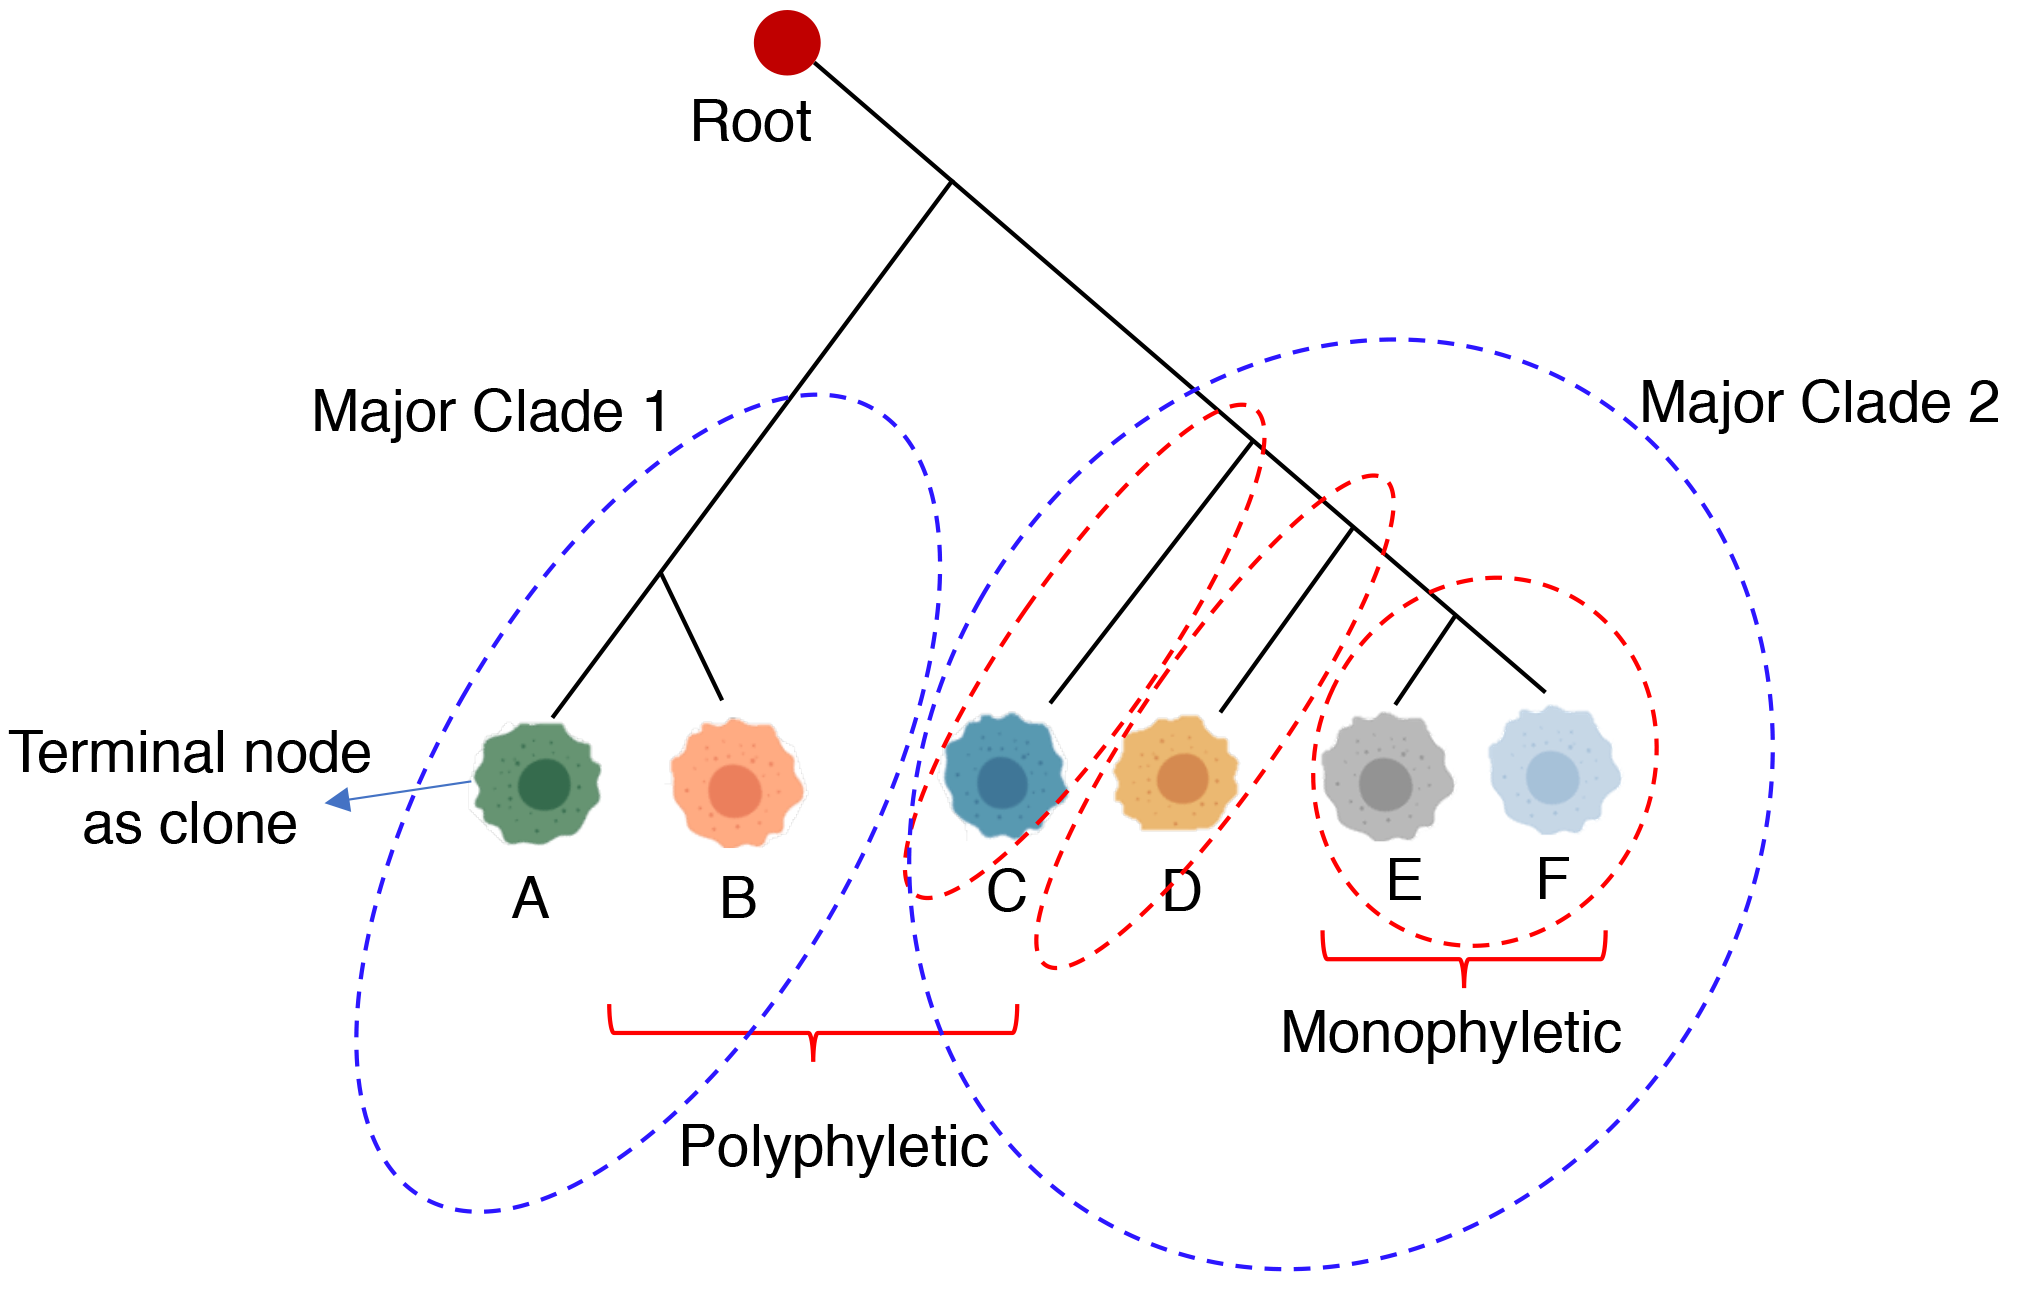
\includegraphics[width=\textwidth]{Figures/chap1/phylogenetictree.png}
	\caption[Diagram of a phylogenetic tree]
	{\small
	    \textbf{Diagram of a phylogenetic tree}.
	 The top red node represents the ancestral node which in rooted phylogentic tree gives rise to new clones in evolving cancer.  Blue dotted circles show major cuts with big clades while red dotted circles show independent small clades. First, left emerging line shows cut in the tree giving rise to monophyletic branch with clone A and B. On right, cut leads to a major clade mentioned as clade 2. Under this major clade more smaller cuts in the phylogenetic tree gives rise to smaller clades that forms polyphyletic tree. Blue dotted circles show major cuts with big clades while red dotted circles show independent small clades.
	}
	\label{fig:phylogentictree}
\end{figure}
 \subsubsection{Phylogenetic representation of clonal evolution and clonal relationship}
Cancers are understood to evolve by mutation of the genome. Decoding cancer evolution approach is essential to understand how therapeutics and progression work, which requires phylogenetics \cite{burrell2013causes, tabassum2015tumorigenesis}. 

The phylogeny of a tumour gives insights into the sequence of events that occurred during tumour evolution but the main challenge is to resolve the subpopulation structure of a heterogeneous tumour sample. Developments in cancer evolution studies and advanced single cell technologies \cite{laks2019clonal} have further  stimulated development of new phlyogenetic methods, building on a rich literature from classical studies of heredity and evolutionary genomics \cite{schwartz2017evolution}. 

A Phylogenetic tree is a diagram that depicts the cell division and inheritance as a branching process whose leaves represent the genotypes observed at the present time and whose internal nodes inferred ancestral genotypes \cite{satas2020scarlet}.
It is useful for organizing the clonal genotypes based on their heritable marks. Tumour cells sharing the same heritable marks, such as, SNV (single nucleotide variation) or CNV (copy number variation), can be grouped into one clone that form the terminal ends of tree. Then, clonal lineage is identified by placing cells with distinct genotypes on the tree branches based on their relationship to each other (using tree cutting methods). A clade represent a part of a tree that includes an ancestral lineage and all the descendants of that ancestor which can be referred to as monophyletic or polyphyletic.  A monophyletic clade can be separated from the root with a single cut, whereas a polyphyletic group needs two or more cuts \textbf{(\autoref{fig:phylogentictree})}. Clones in the same clade share a portion of history that is common to all members of the same clade and different from the clones in other clades \cite{baum2008reading, baum2008phylogenics}.

Certain assumptions are made in the calculation of phylogenetic trees, especially with respect to the appearance and stability of new and existing genotypes over time.
Perfect phylogeny is a term used in computational phylogenetics to denote a phylogenetic tree in which all internal nodes are labeled such that all events (SNV or CNV) evolve down the tree without homoplasy (gain or loss occurring independently in separate lineages over the course of evolution) \cite{gusfield1997algorithms}. Conceptually, the perfect phylogeny model is based on the \textbf{infinite sites} assumption, developed for and largely applicable to single base mutations (SNV), that there are an infinite number of sites  where events can occur. Every new event can occur only once in the whole tree at a novel site and there would be no homoplasy or back mutation. In this model, for example, copy number are gained with low probability (0 to 1 only once), but that are lost with much higher probability (1 to 0 without constraint).

Persistent phylogeny, is an extension of perfect-phylogeny, in which a trait (SNV or CNV) can only be gained once (0 to 1) on the tree, but differs to it in that it allows the trait (SNV or CNV) to be lost exactly once (1 to 0).

In the calculation of phylogenetic trees, \textbf{optimality criteria} are used to determine how closely an inferred tree adheres to the assumptions of the phylogeny:
%\textbf{Optimality criterion} include assumptions that allowed to state that the inferred tree is close to the reality.

\textbf{(a)} Parsimony methods identify the phylogeny that requires the fewest necessary changes to explain the differences amongst observed sequences (the smallest number of steps needed to explain the data). They are considered as model free simplest procedure that imposes minimum restrictions upon permitted event changes. Free reversibility of events is allowed.

\textbf{(b)} Maximum likelihood evaluates evolutionary history in terms of the probabilities of sequences that a proposed model of an evolutionary history with higher probability of giving rise to the observed data is preferred to one with lower probability. 

%\textbf{(ii) Algorithmic methods:} Hierarchical cluster analysis (UPGMA-unweighted pair group method with arithmetic mean) and Neighbour joining:
%These methods estimate a phylogenetic tree by defining a specific sequence of steps that leads to the determination of a tree.

In this dissertation, for the sake of extracting meaningful knowledge from the timeseries data and to understand cancer evolutionary forces acting on clones, we applied a cluster type phylogenetic model that is based on perfect phylogeny and taking presence and absence of changes in the copy number profiles. 
Cluster analysis is different from neighbor joining in that it refers to the ultrametric properties of the tree that includes:

 \textbf{(a)} Branch distance between two taxa is equal to the sum of branches joining them.

\textbf{(b)} Tree is rooted so that all taxa clades are equidistance from the root. The root (usually unlabelled) corresponds to the common ancestor of all clones.

\textbf{(c)} Clock assumptions, that changes occur at the same rate in all lineages at any given time.

Another important concept in phylogenetics is \textbf{phylogenetic distance or branch length} which explains the number of events that are required to go from one node to another. Clock type branch length is important to understand cancer evolution because its important to know at what rates the events are occurring. The phylogenetic model used does not measure clock like rates as these are not understood for CNA and so phylogenetic distance is based on the number of discrete events.

\textbf{Cancer cells can violate the rules of perfect phylogeny.}
The assumptions of perfect phylogeny or persistent perfect phylogeny are more likely to be violated in the data explored in this dissertation. This is because the model of \texttt{sitka} \cite{dorri2020efficient} uses 
 CNA-change points, i.e. markers (breakpoints) instead of integer CNA states as phylogenetic traits. 
While using \textbf{breakpoints (points of copy number change)} as phylogenetic perfect persistence phylogeny model, non-overlapping CNA events do not violate the phylogeny assumptions, but the overlapping events could cause violation by two scenarios in cancer cells:

\textbf{- There could be a copy number gain from an ancestral cell followed  by an overlapping loss event}. This happens in cancers quite often as if chromosome is gained, it could be lost but in perfect phylogeny, \textbf{back mutations} are not allowed. The second loss event would mask or remove the end point of the first event.

\textbf{- There could be a copy number loss followed by an overlapping copy loss}. In cancers, the second overlapping loss event does happen on the same copy as the first. 
All the change in copy number (breakpoints) could occur independently in any lineages which goes against the rule of perfect phylogeny which assumes all events evolve down without homoplasy.  

 \textbf{\texttt{sitka}} (new method of building a phylogeny) assumptions are made to get simplified phylogenetic tree similar to perfect persistence phylogeny, although, the single cancer cell DNA sequencing data could also violate its assumptions:

\textbf{1. There is a change point without noise.} In \texttt{sitka} binary values, 0 and 1 are considered as loss and gain respectively. Violations occur as actually binary values are not observed. Incorrect change point estimates (as a result of noisy HMM CNV calls). 
Markers inconsistent with perfect phylogeny assumptions can be accounted as noise. A complication of parameterizing copy number segments in the genome only with breakpoints, is that a single event could be a small deletion or an entire chromosome. This complicates the interpretation of potential phenotypic impact of genotypes. 


\textbf{2. Infinite site assumptions.} Many infinite events are occurring. Phylogenetic trait arises exactly once on rooted tree topology and all individual cells descending from that position will inherit that trait.
CNV typically occurs at different loci but because of the binning of the data, it could be possible to see two events in the same bin as explained above.

\textbf{3. Considers exact one gain and one loss (perfect persistence phylogeny).} In cancer evolution this scenario doesn't happen as such as explained above, causing the violation.



 
 
 
 %is simplified to the breakpoints of copy number segments. the actual copy number state is not encoded.
 %we are defining clones based on their copy number profiles by using \texttt{sitka (see methods)}, which uses type of perfect phylogeny with same assumptions.

% However,in molecular evolution, if the method of tree construction is measuring single changes of amino acid or a single nucleotide variant (SNV), it could be easy to interpret but if the tree building model is taking CNA as an event then branch length becomes more important.

 Taking change in copy number as an event is more complicated because that single event could be a small deletion or it could be a whole chromosome loss/gain, which in turn has implications in cancer biology. We know that in case of copy number, chromosomal gain can occur independently, which is against the model because it does not allow homoplasy.

If a chromosome is lost, it cannot be regained but if we gain a chromosome, it could be lost, meaning back mutation is possible. Also, it is plausible that events can occur more than once in cancer cells, for example, chromosomal missegregation can occur in mitosis. In this dissertation, we are using the state of gaining a chromosome to mean a genotype, so that could have occurred independently more than once because of the nature of the data itself.

  
%Developments in cancer evolution studies and advanced single cell technologies have further stimulated development of new phlyogenetic methods, building on a rich literature from classical studies of heredity and evolutionary genomics \cite{schwartz2017evolution}.

%A Phylogenetic tree is a diagram that represents the underlying branching process and cell divisions whose leaves represent the cells observed at the present time and whose internal nodes inferred ancestral genotypes \cite{satas2020scarlet}.
%It is useful for organizing the clones based on their heritable marks. 

%Quantification of intra-tumor heterogeneity and evolutionary tree construction plays a role in diagnosis and treatment \cite{burrell2013causes, tabassum2015tumorigenesis}. It provides insights into the sequence of events that occurred during tumor evolution.

%Standard algorithms have been used by majority of studies of tumour phylogenetics that were developed for species phylogenetics (for example, maximum parsimony, minimum evolution, neighbour joining,  UPGMA (unweighted pair group method with arithmetic mean), or various maximum likelihood or Bayesian probabilistic inference methods \cite{de2014spatial, zhang2014intratumor, brocks2014intratumor, navin2011tumour, xu2012single, huelsenbeck2001bayesian, felsenstein2004inferring}. Recent developments in the filed has modified algorithms that are taking into account the specifics to tumor evolution \cite{chowdhury2013phylogenetic, yuan2015bitphylogeny, jahn2016tree}.

%Quantifying intra-tumor heterogeneity and reconstructing the evolutionary history of tumor cells is critical for the diagnosis and treatment \cite{burrell2013causes, tabassum2015tumorigenesis}. Tumor evolution  is typically described by a phylogenetic tree (phylogeny), whose leaves represent the cells observed at the present time and whose internal nodes represent ancestral cells \cite{satas2020scarlet}.
%The phylogeny methods are established on defining certain traits or inherited marks on observed individual cells. The majority of single cell phylogenetic tree inferences focus on point mutations \cite{singer2018single, zafar2017sifit, schwartz2017evolution}. Others markers include \ac{SNV} \cite{bashashati2013distinct}, \ac{CNVs} \cite{navin2011tumour}, DNA methylation, histone marks or RNA expression \cite {brocks2014intratumor, yates2012evolution, greaves2012clonal}.

%Distance based and agglomerative clustering methods such as neighbour joining are scalable and are used to elucidate hierarchical structures over cells \cite{wang2020single, xu2012single}. While useful heuristics, these methods are statistically sub-optimal relative to likelihood based methods \cite{williams2003investigation}.

%A new model applied on the data set used in this dissertation is \texttt{sitka} \cite{dorri2020efficient}, which is based on lossy transformation of single cell copy number matrices retaining only presence or absence of changes in copy number profiles. This transformation turns a complex evolutionary process (integer-valued copy numbers, prone to a high degree of homoplasy and dense dependence structure across sites) into a simpler one which can be approximated by a probabilistic version of an ideal phylogeny .

\subsubsection{Clonal fitness and selection}
%fitness is a quantitative expression of reproducible growth trajectories.  
The tendency of clones to increase or decrease in prevalence under some intrinsic or extrinsic form of selection leads to the idea that the \textbf{fitness} of a clone may be measured by its reproducible growth trajectory. In contrast, \textbf{selection} is an ongoing system that could be transient or stable \cite{szendro2013predictability}.
%Fitness means quantitative measure of ability of specific clonal lineage that undergo directional dynamics over time. 
%Mutation, selection and genetic drift are the three basic processes that defines cancer evolution. \cite{lipinski2016cancer,szendro2013predictability}.

Both fitness and selection are related concepts. Both of which can explain why subpopulations grow and decline, but there is another process which is \textbf{genetic drift}. In population genetics, the basic intuition of \textbf{Wright and Fisher}, is that small natural fluctuations in transmission of alleles during population growth could eventually lead to fixation of one subpopulations, this referred to as \textbf{genetic  drift}. Genetic or stochastic drift attributes to the changes in frequency of an allele in a population due to stochastic random events. Stochastic drift has more prominent effects if the population size is small while it has low impact in larger populations \cite{lynch2007origins}. However, the concept of stochastic drift was first applied on allele frequency in population genetics where meiosis is taking place and stochastic transmission of alleles could occur. In cancer, as there is no meiosis but the principle of stochastic transmission of genotypes still applies and the Wright Fisher model is one way of defining how to estimate it. In the Wright Fisher model, we assume that the total population size is fixed, so the cancer clone that has the higher fitness will grow to occupy a higher clonal fraction faster than the one with a lower fitness.


Fitness, selection and stochastic drift would apply to any population with a fixed number of starting genotypes but the mutation derives the evolution of new genotype. Then resulting new genotypes could get selected overtime \cite{jain2007deterministic,gerrish1998fate}. If a mutation confers a fitness advantage, then eventually selection will mean that it grows in prevalence.
These forms of cellular dynamics play a role in the concept of tumour initiating cells \cite{magee2012cancer} and to some forms of drug resistance \cite{shaffer2017rare, kreso2013variable}. 



\textbf{Alternative methods of identification of neutrality in population genetics have been applied to bulk cancer genome analysis.} 
Two key methods are:

\textbf{(i) The dN/dS ratio test \cite{martincorena2017universal}:} 
The dN/dS ratio test is most widely used method for detecting pattern of natural selection from nucleotide sequence data. It calculates the ratio of the rate of non-synonymous substitutions (dN, the number of non-synonymous substitutions per non-synonymous site) to the rate of synonymous substitutions (dS, the number of synonymous substitutions per synonymous site). Non-synonymous substitutions result in the change in protein sequence while synonymous substitutions change the DNA sequence, but not the protein sequence. These synonymous mutations are used as a baseline to compare the substitutions that do change the protein sequence, that are non-synonymous. The results are inferred as follows:
\begin{itemize}
     \item \textbf{Negative selection: dN/dS ratio <1} (selective constraints on a sequence, fewer substitution that change the protein). 
 \item \textbf{Positive selection: dN/dS ratio >1} (higher proportion of amino acid substitution change).
\item \textbf{Neutral selection: dN/dS ratio = 1} (neutral, free to change without any constraints).
\end{itemize}
This model cannot be applied to our copy number defined clones because there is no concept of a protein coding changes or exact genetic code for the CNV data. Copy number change does not always define the phenotype of tumour cells.


%In this method, SNVs that are present in the non-coding regions of genes (intergenic regions) are identified. It is assumed that these mutations don't change the coding of protein. Even though there is a base variation but because of the genetic code, they don't change the actual protein. These mutations are considered to be neutral. In contrast, if the SNVs are present in the coding regions of a gene, they will not be neutral and the measure of the ratio between them is a measure of fitness and it will infer whether selection is operating \cite{martincorena2017universal}.


\textbf{(ii) Power law in SNV allele prevalances:} This model is based on the relationship of occurrence of mutations as a power law. It demonstrates that neutral tumour evolution results in approximately 1/f power-law distribution, where f is the mutant allele frequency.
A group of mutations in a population can be identified and its prevalence will indicate whether they are behaving in a neutral manner or not \cite{williams2016identification}.

This model could potentially be applicable to our copy number defined clonal data but it does not directly lead to fitness.



\subsection{Single cell whole genome sequencing can reveal molecular dynamics of cellular population fitness in biological systems}
Advancements in identifying the molecular basis of clonal dynamics and evolution by single cell DNA sequencing is unprecedented in cancer research. Conventional bulk DNA sequencing has the advantage of high coverage depth to identify major clones, however, it is limited to resolve minor populations by sequencing error rates \cite{gerstung2012reliable}. 

Large scale single cell genome measurements to scalably define clonal populations in cancer over thousands of cells have only recently emerged, enabling identification of rare populations, precise tracking of clones and robust clone-specific measurements suitable for population genetics modeling  \cite{laks2019clonal,zahn2017scalable}. Several amplification-based methods have been described \cite{navin2011tumour,zong2012genome, hou2012single,ni2013reproducible} but measuring single-cell genomes with \ac{DLP+} in tissues and cell populations has greatly advanced clonal decomposition of malignant tissues. 
Moreover, help studying properties of negative selection, resolving rare cell population genotypes and identifying DNA replication states of individual cells, all of which are hard to measure when cellular information is destroyed in bulk sequencing. 

Cellular fitness underpins the tissue population dynamics of cancer progression and treatment response. Yet, quantifying fitness in heterogeneous cell populations and identifying causal mechanisms shaping fitness landscapes remain open problems. In particular, quantitative fitness modelling of cancer cells has numerous and diverse implications; attributing clonal dynamics to drift or selection, identifying the determinants of clonal expansion, enabling causal inference, and forecasting growth trajectories. 

\subsubsection{Measurement of fitness of sub-population in growing cancers}

CNA determined clonal evolution has not been well studied due to lack of scalable methods for single cell CNA measurement.

To identify and quantify fitness based on sub-population in growing cancers require: 

\textbf{(i) Method for identifying sub-populations with their genotypes}.
Variation in mitotic mis-segregation rates across tissue types and genotypes could be defined from DLP+. Moreover, analysis of matched genomic measurements could reveal correlations between cellular morphology and genome ploidy states. Consequently, aggregation of cells sharing copy number profiles allowed for calculation of single-nucleotide resolution, clonal genotypes and inference of clonal phylogenies.
Limitations of this approach to structural and copy number genotypes arise from inability to resolve populations accurately. Defects in genome maintenance leads to accumulations of chromosomal aberration, including \ac{CNA} which is an evolving hallmark of cancer \cite{negrini2010genomic}. 


Single cell sequencing technology opens up the opportunity to accurately identify CNA, structural sub-populations that in turn gives clonal relationship with phylogenetic reconstruction \cite{satas2020scarlet, dorri2020efficient}. 

\textbf{(ii) Serial or repeated sampling of the populations}.
We know from population genetics that it is possible to measure quantitatively the tendency of populations with shared genotypes to experience differential growth and survival, i.e., the \textbf{fitness of genotypes}, from population samples drawn \textbf{over time}.
These two concepts can be linked to measure the fitness associated with copy number assigned clones identified by a novel scWGS method (DLP+), in serially sampled tumours.

\textbf{(iii) A method for estimating the likelihood, the trajectory is non neutral}.
These estimations involve mathematical and statistical models to actually quantify and infer the fitness of any clonal population showing dynamical behaviour over time.


\section{Studying cancer dynamics by single cell RNA sequencing}

Differences between cancer cells could arise by hardwired changes in the genome, or by epigenetic/transcriptional reprogramming which may be transient, if the stimulus or condition is transient. 
As noted above that fixed changes in the genome can lead to changes in gene expression and copy number segment changes themselves can change gene expression.
However, gene expression can differ between cells independently of genomic alterations, for example by epigenetic reprogramming or selection of rare states of gene expression.

Single cell transcriptome sequencing has increased in feasibility, decreased in cost and is appropriate to advancing our understanding in this area, for example, the ability to assign expression states to subpopulations of cells sharing genomic attributes. \textbf{\textit{in cis}} regulated genes refer to the gene expression modulated by change in copy number. \textbf{{\textit{in cis} positive linear tendency}} means if the gene expression is up regulated with the gain in copy number, whereas, \textbf{{\textit{in cis} negative tendency}} means that the gene expression is paradoxically changing with change in copy number. However, \textbf{\textit{in trans}} genes are independent of copy number change.

Recent advances in understanding transcription and its role in tumour phenotype suggest that the clinical progression and therapeutic responsiveness, are likely to be strongly regulated by the dysregulated versions of ongoing transcriptional programs within the cancer cells \cite{lawrence2014discovery, sur2016role}. Therefore, its critical to understand the factors altering the gene expression.

\subsection{Linking gene expression states to genetic or non-genetic alterations}
It is broadly acknowledged that somatic CNV is highly associated with the development and progression of numerous cancers by influencing gene expression profiles \cite{yang2017prame, gut2018sox2}. 
Developments in single cell sequencing technologies over the last decade now allow for scaled single cell transcriptome profiling \cite{zahn2017scalable, zheng2017massively}.
By now, extensive single cell cancer genome sequencing studies have revealed changes in genome that affect nearly every component of normal transcriptional control \cite{garraway2013lessons}. 
Bhattacharya \textit{et al.} studied that CNV can promote tumour progression through alteration of gene expression levels genes located at the affected genomic regions \cite{bhattacharya2020transcriptional, henrichsen2009segmental, tang2013gene}. Furthermore, Stranger \textit{et al.} revealed that a copy number alterations of genomic segments at a given position of the human genome may affect not only locus and adjacent gene expression but also genome regulation and pathways contributing to a change in phenotype \cite{stranger2007relative}. However, transcription can be altered as a result of epigenetic modifications that could lead to fixed selection. Epigenetics refers to both heritable changes in gene activity and expression and also stable, long-term alterations in the transcriptional potential of a cell that are not necessarily heritable \cite {aristizabal2020biological, nih2019overview}.
One of the recent studies, used single cell RNA sequencing measuring tools, showed that the addition of drug induces epigenetic reprogramming in cancer cells leading to selection of fixed selection \cite{shaffer2017rare}. Moreover, this study showed that there could be fluctuations of transcriptional states of cancer cells, for example, the resistant phenotype in the presence of drug is not fixed and not inherited, but once the state got selected and fixed, the reversibility is not possible, converting the transient transcriptional state to a stably resistant state. Furthermore, another study showed that the two subpopulations of cells were stable in that they do not interconvert between the two expression patterns. Also, it was revealed that those two subpopulations exhibited distinct methylation patterns at their imprinting control regions \cite{ginart2016visualizing}.


\subsection{Scaled single cell RNA sequencing}
 Conceptually, single cell RNA sequencing is a multi-stage process starting from single cell preparation, cell capture, efficient cell lysis, transcript capture, reverse transcription, cDNA preamplification, and final cDNA library construction suitable for high-throughput DNA sequencing.
 At present there are four commercial scRNA-seq platforms available: 
(i)	Fluidigm C1 
(ii)	WaferGen/Takara iCell8 
(iii)	10X Genomics Chromium Controller
(iv)	Illumina/BioRad ddSEQ.
Interestingly, all these platforms have a high degree of specificity on protein coding regions of transcripts and highly variable genes significantly overlap across platforms \cite{ashton2020comparative}. However, these single cell RNA plateforms vary in number of single cell throughput from 96 to 80,000 single cells. The number of successfully sequenced cells could also be influenced by many factors, such as quality of cell suspension, percent viability in single cell suspension and cell type \cite{o2019dissociation}. 

10X Genomics platform was used for the single cell RNA sequencing done for this dissertation. 10x Genomics' single-cell RNA-seq (scRNA-seq) technology uses microfluidic partitioning to capture single cells and prepare barcoded, next-generation sequencing (NGS) cDNA libraries. Gel Beads containing barcoded oligonucleotides, and oil are combined on a microfluidic chip to form reaction vesicles called Gel Beads in Emulsion (GEMs). Each functional GEM contains a single cell, a single Gel Bead, and reverse transcriptase (RT) reagents. Within each GEM reaction vesicle, a single cell is lysed, the gel bead is dissolved to free the identically barcoded RT oligonucleotides into solution, and reverse transcription of polyadenylated mRNA occurs. Therefore, all cDNAs from a single cell will have the same barcode that could be mapped back to their original single cell. According to vendor the recovery rate from 10X genomics platform is around 65\%.

The challenge in the field of studying cancer dynamics by single cell RNA sequencing is to understand the genome driven expression vs non-genomic. A best way to design controlled experiments in such a way to get simultaneous and repeated measurements of genome or methylome with single cell RNA expression. In this dissertation we have partially addressed this by elucidating copy number driven expression in clones.



%%%%%%%%%%%%%%%%%%%%%%%%%%%%%%%%%%%%%%%%%%%%%%%%%%%%%%%%%%%%%%%%%%%%%%
\section{Thesis goals and Scientific questions}

\subsection{Overarching goal}

The overarching goal of this dissertation is to measure the copy number defined clonal fitness with and without drug pressure over time in breast cancer and to understand its phenotypic impact.


\subsection{Objectives}
\begin{itemize}
\item{To set up and identify drug resistance patterns in transplantable breast cancers}

\item{To identify technical conditions for single cell dissociation}

\item{To determine fitness after drug resistance induction and ask which clones are selected and confirm whether this is reproducible}. 

\item{To identify what proportion of the clone phenotype might be driven by \textit{cis} vs \textit{trans} in transcript phenotypes} 

\end{itemize}

In this thesis, we have used all different types of breast tumours for testing transplant capability and initial screening in chapter 3.  However, for chapter 4 and chapter 5, only \ac{TNBC} were selected to create timeseries forced amplified evolution models under chemotherapy selection to determine the cellular mechanisms in resistance  at single cell resolution.

 We have used \ac{scWGS} and scRNA-seq techniques to define the population dynamics in re-transplantable TNBC PDX.
 Since TNBC PDX are especially dynamic and exhibit genomic instability, a longitudinal tracking of tumour passages in PDX provides insights into the stability of genome instability patterns, as well as clonal transcriptional states over genomic clones.
 
 In \textbf{Chapter 3}, established a transplant model and the methods for single cell dissociation. PDX generations, protocol development, optimizations and \textit{in vivo} screening. 
 
 In \textbf{Chapter 4}, identified patterns of clonal resistance and sampling from populations using single cell DNA sequencing to measure the fitness over clones.
 
 In \textbf{Chapter 5}, identified resistance phenotypes by longitudinal scRNA sequencing and characterization of differentially  expressed genes and pathways.



%    2. Main body
%%%%%%%%
\chapter{Methods and Materials}

\section{Ethical approval}
The Ethics Committees at the University of British Columbia approved all the experiments using human resources. Patients in Vancouver, British Columbia, undergoing excision or diagnostic core biopsy were recruited, and samples were collected after written consent, under the tumour tissue repository (TTR-H06-00289) protocol and transplanted in mice under the Neoadjuvant patient derived xenografts (PDX) (University of British Columbia BC Cancer Research Ethics Board H20-00170) protocols. All experimental methods comply with the Helsinki declaration. All animal studies were approved by the Animal Care Committee at the University of British Columbia.  


\section{Establishment of patient derived xenografts} 
Patient's tumor materials were processed as described in \cite{eirew2015dynamics} and transplanted in mice under the \ac{ARC} bioethics protocol (A19-0298-A001) approved by the animal care committee.
Briefly, tumour fragments were chopped finely with scalpels and mechanically disaggregated for one minute using a Stomacher 80 Biomaster (Seward Limited, Worthing, UK) in \SIrange{1}{2}{\ml} cold DMEM/F-12 with Glucose, L-Glutamine and HEPES (Lonza 12-719F).
An aliquot of \SI{200}{\ul} of medium (containing cells/organoids) from the resulting suspension was used equally for 4 transplantations in mice.

Tumours were transplanted in mice as previously described~\cite{eirew2015dynamics} in accordance with SOP BCCRC 009. 
Briefly, female immuno-compromised, NOD/SCID/IL2r$\gamma^{\small{-/-}}$\ac{NSG} and        
\ac{NRG} \cite{pearson2008non} mice were bred and housed at the animal resource centre \ac{ARC} at the British Columbia (BC) Cancer Research Centre . 
For subcutaneous transplants, mechanically disaggregated cells and clumps of cells were re-suspended in \SIrange{150}{200}{\ul} of a 1:1 v/v mixture of cold DMEM/F12: Matrigel (BD Biosciences, San Jose, CA, USA).
8-12 weeks old mice were anesthetized with isofluorane, then the mechanically disaggregated cells/clumps suspension was injected under the skin on the left flank using a \SI{1}{\ml} syringe and 21gauge needle. 
The animal care committee and animal welfare and ethical review committee, the University of British Columbia (UBC), approved all experimental procedures.

\subsection{Histopathology of PDX tumours} 
The hormone receptor status of most of the tumour samples was determined by immunohistochemistry and FISH (Fluorescence in situ hybridization) copy number.
Two separate tissue microarrays were prepared using duplicate \SI{1}{\mm} cores extracted from formalin-fixed paraffin-embedded blocks containing material from all passages of the patient derived xenografts (3 TNBC and HER2+) used for this project. 
Deparaffinized \SI{4}{\um} sections of paraformaldehyde fixed tumours were processed for immunohistochemistry (IHC) using a Discovery XT automated system (Ventana Medical Systems, Tucson, AZ, USA). 
EGFR, INPP4B, Ki67, PR, ECAD were all performed on the Ventana Discovery XT platform using CC1 for antigen retrieval, incubating for one hour at room temp, and using the UltraMap DAB detection kit.
Primary antibodies to ER$\alpha$ (clone SP1, Ventana), HER2 (clone 4B5, Ventana), EGFR (clone EP22, Epitomics, Burlingamen, CA, USA) and Ki67 (clone SP6, Thermo Scientific) 
Horseradish peroxidase-conjugated Discovery Universal Secondary Antibody (Ventana) was then applied and the slides developed using 3,3’-diaminobenzidine Map Kit (Ventana). 
The slides were reviewed by a pathologist. Representative images from SA609 TNBC and HER+ PDX early and late passages are shown in \textbf{\autoref{fig:HistologyHER2+TNBC}}. These images indicates that in our PDX model system, the tumors retain architecture and receptor markers from early to late passages.


 \begin{figure}
\centering
\includegraphics[width=\textwidth]{Figures/HistologyHER2+TNBC.png}
	
\caption[Untreated PDX timeseries and growth trajectories]
	{\small
\textbf{Representative patterns of expression on histology in early and late passages.}
 \textbf{(a)}, IHC of HER2+ tumours at passage 1 (X1) and passage 10 (X10), 4x and 20x (insets). Scale bars \SI{500}{\micro\metre} and \SI{100}{\micro\metre} (insets). On top of each panel presenting the antibody name and the right bottom square is showing the score of the stain.
\textbf{(b)} IHC of TNBC SA609 tumors at passage 2 (X2) and passage 10 (X10), 4x and 20x (insets). Scale bars \SI{500}{\micro\metre} and \SI{100}{\micro\metre} (insets). On top of each panel presenting the antibody name and the right bottom square is showing the score of the stain.}
	\label{fig:HistologyHER2+TNBC}
\end{figure}


Sections were deparaffinized in xylene, rehydrated in graded alcohol, and used for histology and immunostaining. 
H \& E and \ac{IHC}  of the two PDX tumours showed that TNBC is  derived from a triple negative breast cancer patient while HER2+ was derived from a HER2+ breast cancer patient. HER2 IHC was scored as 2+, HER2/CEP17 ratio was calculated as 6.5 (positive)\cite{ahn2020her2} from  \ac{FISH}  and focal high level amplification (average copy number state of 10) of the \ac{ERBB2} locus (approximately Chr17:37500001-38000000) was found in the DLP+ data.

\begin{table}
\centering
\caption{List of antibodies and experimental conditions.}
Summary of antibodies clones and their suppliers used for staining TMAs for IHC.

\small\textbf{(*RTU: Ready to use; N/A: not applicable)}.
\label{stab:antibodieslist}
\begin{tabular}{|rl|l|l|l|}
  \hline
 & Specimen & Stain/IHC & Vendor / Ab Clone & Dilution  \\ 
  \hline
1 & TMA1 \& 2 & CK14 & Empire Genomics clone LL002 & 1 in 50 \\ 
  2 & TMA1 \& 2 & Ck5/6 & Dako D5/16 B4 & *RTU  \\ 
  3 & TMA1 \& 2 & Ck8 (CAM5.2) & BC Bioscience CAM5.2 & 1 in 10  \\ 
  4 & TMA1 \& 2 & EGFR & Epitomics 1902-1 & 1 in 100  \\ 
  5 & TMA1 \& 2 & ER & Ventana  clone SP1 & *RTU\\ 
  6 & TMA1 \& 2 & H\&E & *N/A & *N/A \\ 
  7 & TMA1 \& 2 & INPP4B & Abcam EPR3108Y ab81269 & 1 in 50 \\ 
  8 & TMA1 \& 2 & Ki67 & Abcam ab16667  & 1 in 400  \\ 
  9 & TMA1 \& 2 & PR & Abcam ab30285 & 1 in 200  \\ 
  10 & TMA1 \& 2 & Slug/Snail & Abcam ab85936 & 1 in 125 \\ 
  11 & TMA1 \& 2 & SMA & Dako clone 1A4 & 1 in 100 \\ 
  12 & TMA1 \& 2 & Trichrome & Sigma-HT15-1KT & *N/A \\ 
  13 & TMA1 \& 2 & Twist & NB120-49254 & 1 in 200\\ 
  14 & TMA1 \& 2 & Vimentin & Dako V9 & RTU  \\ 
  15 & TMA1 only & E-Cad & Cell Signal 3195 & 1 in 100  \\ 
  16 & TMA1 only & HER2 & Roche 4B5 & 1 in 8  \\ 
  17 & TMA2 only & E-Cad & Dako NCH-38 & *RTU  \\ 
  18 & TMA2 only & HER2 & Ventana  clone 4B5 & *RTU \\ 
   \hline
\end{tabular}%
\end{table}

\subsection{Serial passaging of PDX}
Tumours were serially passaged as  described \cite{eirew2015dynamics}.
Briefly, for serial passaging of PDX, xenograft-bearing mice were euthanized when the size of the tumours approached \SI{1000}{\mm\cubed} in volume (combining together the sizes of individual tumours when more than one was present).
The tumour material was excised aseptically, then processed as described for primary tumour. 
Briefly, the tumour was harvested and minced finely with scalpels then mechanically disaggregated for one minute using a Stomacher 80 Biomaster (Seward Limited, Worthing, UK) in \SIrange{1}{2}{\ml} cold DMEM-F12 medium with Glucose, L-Glutamine and HEPES. 
Aliquots from the resulting suspension of cells and fragments were used for xenotransplants in next generation of mice and cryopreserved.
Serially transplanted aliquots represented approximately 0.1-0.3\%  of the original tumour volume. HER+ and TNBC PDX were passaged upto 10 generations and scWGS was carried out at each timepoint while scRNAseq was done at initial, mid and late timepoint. 

\subsection{TNBC PDX tumour mixing experiments} Frozen untreated passages three (X3) and eight (X8) vials from TNBC PDX, were thawed and  physically remixed in two different volumetric proportions of X3:X8 by tumour weight at the ratio of approximately 1:1 and 1:0.4, labelled as mixture branch a and branch b, respectively. From each of different dilutions, \SI{200}{\ul} of aliquot was taken to be used to transplant in two mice each using the same protocol of transplantation as described above. Before transplantation a small proportion of the physical mixture of cells, from the 1:1 ratio, was subjected to whole genome single cell sequencing to measure the baseline clonal composition labelled as M0 and its subsequent PDX as M1 \textbf{\autoref{fig:Mixturenew} a)}. Each of the thawed X3 and X8 cell populations used for mixing were also transplanted independently to confirm the viability of the tumour material for PDX tumour growth. The tumour cell mixture was then serially passaged over 4 generations, designating the transplants as M1-M4. Tumours from each X3:X8 serial passages from both mixture branches were collected and analysed with scWGS (DLP+) as for other samples.

\subsection{TNBC PDX timeseries treatment with chemotherapies}
\label{ssec:rx}
NRG mice of the same age and genotype as above were used for transplantation treatment experiments. Drug treatment with cisplatin (Platinum) was commenced when the tumour size reached approximately \SIrange{300}{400}{\mm\cubed}. Cisplatin (Accord DIN: 02355183)  was administered i.p. at \SI{2}{\mg\per\kg} every third day for 8 doses maximum (Q3Dx8). The dosage schedule was adjusted 50\% less than what is mentioned in the literature \cite{li2013enhanced,wang2013klotho} and around one third of the maximum tolerated dose (MTD) calculated in the immunodeficient mice  \textbf{(\autoref{fig:treatmentdesignMTD} b)} . Low dose cisplatin pulse and tumour collection timings were optimized to achieve the experimental aims of tumour resistance. The aim was to collect tumour at 50\% shrinkage (from the starting tumour at the time treatment started) in size when measured with a caliper. Cisplatin \SI{1}{\mg\per\ml} was diluted in 0.9\% NaCl to obtain concentrations \SI{200}{\ul}/\SI{20}{\g} of mouse weight and kept in glass vials at room temperature. Quality control \ac{QC} samples were prepared freshly on each day prior to the dosing. Mice were continually monitored for acute signs of toxicity including pain at injection site, skin tenting, coat scruffing, sunken eyes, food consumption and behaviour for the first two hours following compound administration. For TNBC PDX, 8 mice at initial passage were transplanted in parallel for the treatment/treatment holiday study group. Half of the mice were treated with cisplatin when tumours exhibited around 50\% shrinkage, the residual tumour was harvested as above and re-transplanted for the next passage in the group of eight mice. Again, half of the mice at X5 were kept untreated while the other half were exposed to cisplatin following the same dosing strategy. Four cycles of cisplatin treatment were generated, with a parallel drug holiday group at each passage. Cisplatin treated tumours were coded as \textit{UT, UTT, UTTT, UTTTT} for each of the four cycles of drug respectively, while the tumours on drug holiday were labelled as \textit{UTU, UTTU} and \textit{UTTTU} for the three timepoints. Each number of \textit{T} exhibits the number of cycles of drug exposure. SA535 TNBA PDX was also treated with CX5461, the same way like cisplatin. CX-5461 was dissolved in 50mM NaH2PO4, pH4 for xenograft application. CX-5461 was administered through oral gavage once every three days at the final dose of \SI{50}{\mg\per\kg}.
Sc-WGS and scRNAseq was carried out from each tumour during the timeseries treatment with counterpart drug holiday and untreated controls  \textbf{(\autoref{fig:treatmentdesignMTD} a)}.

\begin{figure}
\centering
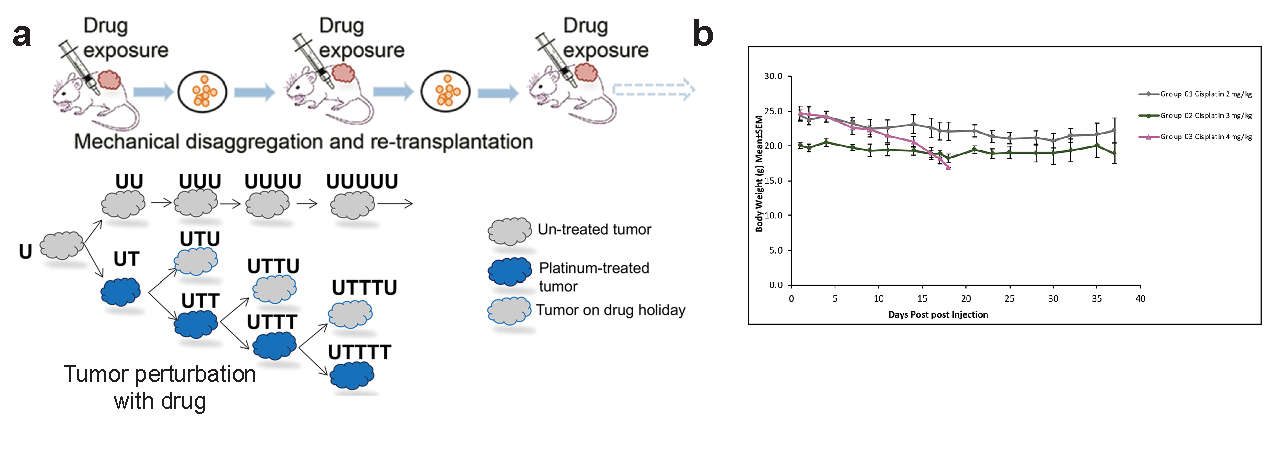
\includegraphics[width=\textwidth]{Figures/treatmentdesignMTD.pdf}
	
\caption[Experimental overview of TNBC PDX treated time series]
	{\small
	\textbf{Experimental overview of treatment design in TNBC PDX time series}
\textbf{(a)} Experimental design of cisplatin treatment in PDX.The residual tumour from one treated mouse was re-transplanted in the next (n=8). The solid blue colour represent cisplatin treated tumours \textit{(UT, UTT, UTTT, UTTTT)}; blue outlined in grey represents drug holiday \textit{(UTU, UTTU, UTTTU)}. Grey represent the untreated series \textit{(U, UU, UUU, UUUU, UUUUU)} \textbf{(b)} Mouse body weight graph recorded during \ac{MTD} evaluation of cisplatin in NRG mice (n=3 in each study cohort).}
	
	\label{fig:treatmentdesignMTD}
\end{figure}


\subsection{PDX tumour growth measurement curves} 
NRG mice received sub-cutaneous inoculation (SQ) of tumour cells (\SI{150}{\ul}) on day 0. 
The tumours were allowed to grow to palpable solid nodules.
Around 7-9 days after they are palpable, their size were measured with calipers every 3rd day. 
tumours were measured in two dimensions using a digital caliper and expressed as tumour volume in mm3; defined as: [volume= 0.52$\times$(Length)$\times$(Width)].
Under drug perturbation, the treated tumours in the first two cycles of treatment showed rapid growth reduction but in third cycle started showing non-responsive behaviour leading to total resistance in fourth cycle 



\section{PDX tumor dissociation into single cells}

\subsection{Tissue dissociation at 37\textdegree C}
Tumour fragments from patient breast and ovarian samples and PDXs were incubated for 2 hrs with a collagenase/hyaluronidase enzyme mix in serum-free Dulbecco's Modified Eagle's Medium (DMEM) at 37\textdegree C with intermittent gentle trituration with a wide bore pipette tip. Cells were resuspended in 0.25\% trypsin-edta for 1 min followed by neutralization with 2\% FBS in Hank's Balanced Salt Solution (HBSS) and centrifugation. Cells were resuspended in 2\% FBS/HBSS and filtered through a 40\textmu m filter. Where necessary, dead cells were removed using MACS Dead Cell Removal Beads (Miltenyi Biotec) according to the manufacturer's instructions. Cells were centrifuged and resuspended in 0.04\%  BSA/PBS and cell concentration adjusted for scRNAseq. For timecourse experiment, tissue was dissociated as above for 3 hrs with samples taken at 30 mins, 1 hr and 2 hr.

\subsection{Tissue dissociation at 6\textdegree C}
Tumour fragments were incubated for 30 minutes at 6\textdegree C with a serine protease, subtilisin A, derived from the Himalayan soil bacterium \textit{Bacillus Lichenformis} (Creative Enzymes NATE0633) in PBS supplemented with 5mM CaCl2 and 125U/ml DNAse, as described in \cite{adam2017psychrophilic, potter2019dissociation}. During dissociation, samples were gently triturated every 5 minutes using a wide-bore pipette. Cells were resuspended in 0.25\% trypsin-edta for 1 minutes at room temperature, neutralized with 2\% FBS in HBSS and filtered through a 40\textmu m filter. Following dissociation, samples were processed for scRNAseq as described above. For the timecourse experiment, tissue was dissociated as above for 3 hours with samples taken at 30 minutes, 1 hour and 2 hours. 

\subsection{Removal of murine contamination from patient derived xenograft samples}

To identify murine cells in the PDX samples, we re-ran CellRanger version 3.0.2 aligning cells to both GRCh38 and mm10 (separately). We then considered all cells for which a valid barcode was identified in the raw (unfiltered) data for either alignment, and counted the number of reads mapping to each genome for each cell. A cell was subsequently designated as a contaminating mouse cell if more reads mapped to mm10 than GRCh38, and a human cell otherwise.

\section{\textit{in vitro} cultures and assays}

\section{chemotherapies}
For \textit{in vitro} assays, the chemotherapies used are summarized in table.


\subsection{WST-1 assay}
In all the experiments in \textbf{\autoref{fig:invitro}}, the cell viability was measured by WST-1 assay according to the protocol provided by manufacturer (Roche, Catalogue number 11644807001). Single cells from PDX and Wild type and HCT116 (DNA-PK and Lig4 knockout) cells were plated in 96-well plates either untreated or treated with drug continuously during the indicated time before WST-1 assay. Drug incubation time was 6-7 days. Absorbance was read with the microplate reader SpectraMax 3 (Molecular Devices, Sunnyvale, CA, USA).

\subsection{Dose response curve fitting for cell line WST-1 assay}
Where sigmoid curves were appropriate for dose response analysis, a four-parameter logistic regression curve was fitted to the data using the R function ‘nlme’. An IC50 was estimated, the difference in IC50 values was calculated for conditions with and without drug. The set of differences was tested using the Student's paired t-test.

\section{Live/dead cells analysis}

\subsection{Flow Cytometry for live/dead cells staining}
 GM18507 cells were treated with or without 100ng/ml TNF\textalpha for 24 hours before being stained with propidium iodide (catalogue no.P1304MP, Theromofisher scientific) and FITC annexin V (catalogue no.640905, Biolegend) and sorted into dying, dead or live populations according to single, double or negative staining respectively using a FACS Aria Fusion (BD Biosciences).
 
\subsection{Clustering of live, dying, and dead cells}
Cells were hierarchically clustered using the \texttt{hclust} function in \texttt{R} applied to the 10-dimensional output of MNN, and clusters assigned using the \texttt{cutree} function.

\subsection{Reproducible data analysis}
A dockerized workflow to enable reproduction of all figures and analysis in this paper is available (Campbell, K. kieranrcampbell/scrnaseq-digestion-paper. Github. \url{https://github.com/kieranrcampbell/scrnaseq-digestion-paper}(2019). Corresponding docker image is at \url{https://cloud.docker.com/u/kieranrcampbell/repository/docker/kieranrcampbell/statgen2} (version 0.4).

\section{Single cell whole genome sequencing and library construction with DLP+}

All libraries, including metrics on number of cells, average number of reads per cell and quality control metrics are listed in refsuptab{tab:omnibusMedians}.

\subsection{Creation of single cell suspensions from PDX}
Tumour fragments from PDX samples were incubated with a collagenase/hyaluronidase 1:10 (10X) enzyme mix (STEM CELL technologies, Catalog \#07912) in  \SI{5}{\ml} DMEM/F-12 with Glucose, L-Glutamine and HEPES (Lonza 12-719F)and 1\%BSA at \SI{37}{\degreeCelsius} with intermittent gentle pipetting up and down the sample every 30 min for 1 min, during the first hour with a wide bore pipette tip, and every 15-20 min for the second hour, followed by  centrifugation (1100 rpm, 5 min) and supernatant removal.
The tissue pellet was resuspended in \SI{1}{\ml} of  0.25 percent trypsin-EDTA (VWR CA45000-664) for 1 min, superadded by \SI{1}{\ml} of DNAse 1/dispase \SI{100}{\ul}/\SI{900}{\ul} (StemCell 07900,00082462) pipetted up and down 2 min, followed by neutralization with 2\% FBS in HBSS with 10 mM HEPES (STEMcells Catalog \#37150). 
This cell suspension was then passed through a \SI{70}{\micro\metre} filter to remove remaining undigested tissue and centrifuged for 5 min at 1100 rpm after topping it up to \SI{5}{\ml} with HBSS.
Single cells pellet  was resuspended in PBS + 0.04\% BSA (Sigma) in appropriate volume to achieve  $\approx$~1 million per ml concentration of cells for robot spotting for DLP+.

\subsection{Robot spotting of single cells into the nanolitre wells and library construction}
scWGS DLP+ library construction was carried out as described in \cite{laks2019clonal}. Briefly, single cell suspensions from cell lines and patient derived xenografts were fluorescently stained using CellTrace CFSE (Life Technologies) and LIVE/DEAD Fixable Red Dead Cell Stain (ThermoFisher) in a PBS solution containing 0.04\% BSA (Miltenyi Biotec 130-091-376) incubated at \SI{37}{\degreeCelsius} for 20 minutes. Cells were subsequently centrifuged to remove stain, and resuspended in fresh PBS with 0.04 percent BSA. This single cell suspension was loaded into a contactless piezo electric dispenser (sciFLEXARRAYER S3, Scienion) and spotted into the open nanowell arrays (SmartChip, TakaraBio) preprinted with unique dual index sequencing primer pairs. Occupancy and cell state were confirmed by fluorescent imaging and wells were selected for single cell copy number profiling using the DLP+ method \cite{laks2019clonal}. Briefly, cell dispensing was followed by enzymatic and heat lysis. After cell lysis, tagmentation mix 
(\SI{14.335}{\nano\liter} TD Buffer, \SI{3.5}{\nano\liter} TDE1, and \SI{0.165}{\nano\liter} 10\% Tween-20) in PCR water were dispensed into each well followed by incubation and neutralization. Final recovery and purification of single cell libraries was done after 8 cycles of PCR. Cleaned up pooled single-cell libraries were analyzed using the Aglient Bioanalyzer 2100 HS kit. Libraries were sequenced at UBC Biomedical Research Centre (BRC) in Vancouver, British Columbia on the Illumina NextSeq 550 (mid- or high-output, paired-end 150-bp reads), or at the GSC on Illumina HiSeq2500 (paired-end 125-bp reads) and Illumina HiSeqX (paired-end 150-bp reads). The data was then processed to quantification and statistical analysis pipeline \cite{laks2019clonal}.

\section{Single cell whole genome data analysis}
\subsection{DLP+ sequence analysis, copy number determination and quality control filtering}
FASTQ pre-processing, sequence alignment, quality control, copy number calling and S-phase classification and filtering was performed on all libraries as detailed in \cite{laks2019clonal}. Briefly, cells were assigned a quality score (QS) for data quality based on a 13 feature Random forest classifier fitted and applied as per \cite{laks2019clonal}. Copy number alterations on a per cell basis were determined using a hidden Markov Model (HMM) approach using the \texttt{HMMCopy} package with parameterizations detailed in \cite{laks2019clonal}. S-phase cells were identified using an automated classifier trained using cell-cycle sorted cells and where features from HMM output were used to identify cells most probably in early or late phase replication of their genomes. As these cells interfere with downstream phylogenetic analysis, they were removed from the analysis according to parameter settings and thresholds established in \cite{laks2019clonal}. To further enable phylogenetic inference, 10-15\% of cells with highest average copy number state jumps were removed. Upon inspection, these cells included early and late dividing cells that were not captured by the s-phase classifier. 
Attrition of cells at each stage of quality control is shown in (suptabtab:omnibusMedians).



\subsection{Identifying clones through phylogenetic analysis}
Using sitka we established the evolutionary relationships of cells in a PDX heterogeneous samples. To investigate cancer evolution we need to determine the abundance of subpopulations over time. To this end, we introduce \texttt{Lumberjack}, a tree-cutting algorithm that we used to define clonal subpopulations. In the output tree of \texttt{sitka}, cells are part of the terminal leaf nodes of the phylogenetic topology. We post-processed the inferred trees to identify clonal populations from major clades. When clonal populations are defined, their abundances were counted as a function of timeseries and these were used for fitness inference. 
Clones are constructed by identifying connected components (each a clade or a paraphyly) in the phylogenetic tree reconstruction. The tree is `cut' into discrete populations according to the following procedure

\subsection{Phylogenetic tree inference, clone determination and clonal abundance measurements}

We developed a single cell Bayesian tree reconstruction method based on copy number change point binary variables called \texttt{sitka} \cite{dorri2020efficient} to fit phylogenetic trees to the copy number profiles.  
In the output of \texttt{sitka}, cells are the terminal leaf nodes of the phylogenetic topology.  
The inferred trees were post-processed to identify clonal populations from major clades. With clonal populations defined, their abundances were counted as a function of timeseries and these were used for fitness inference (see below). 
Clones were constructed by identifying connected components (each a clade or a paraphyly) in the phylogenetic tree reconstruction. The tree was `cut' into discrete populations according to the following procedure (see Algorithm \cite{salehi2020single}).
%%Notation
Let $L$ be a set of loci and $C$ a set of cells and ${\lvert}L{\rvert}$. 
Define $\tau = (L, C, E)$ to be a rooted phylogenetic tree with $E$ its set of directed edges.
The phylogenetic tree is assumed to comprise internal nodes that are phylogenetic markers (loci) and terminal nodes that are either cells or loci. 
Terminal loci are considered unused phylogenetic markers and are discarded. 
Let ${\lvert}\tau{\rvert} = {\lvert}C{\rvert}$, that is the number of cells that belong to tree $\tau$.
By $\tau_{l} = (L_l, C_l, E_l)$ denote the subtree rooted at node $l$.
Set $\text{pa}(l)$ and $\text{child}(l)$ be the parent node and set of immediate children of node $l$ with $\text{desc}(l)$ comprising all its descendant. 

% Final clone determination
The inputs to the algorithm are the rooted phylogenetic tree $\tau$ and the copy number states of its cells.
A clone is defined as connected components (each a clade or a paraphyly) in the graph tree $\tau$ composed of cell of sufficient genomic homogeneity. 
The degree of homogeneity can be tuned by limiting the number of loci and the difference in copy number of sub-clades in a clone. 
The algorithm works by first finding the coarse structure, that is dividing the tree into major clades and then looking for fine structures within each clade by traversing the tree in a bottom up manner and merging loci that are sufficiently similar.
The remaining loci constitute the roots of detected clades.

% First pick coarse structures
To obtain the coarse structure from the reconstructed phylogenetic tree we use a two step procedure. (i) First we identify monophyletic clades via algorithm \cite{salehi2020single}. 
(ii) We then remove the cells comprising the clades found in step one from the tree and repeat algorithm. 
We note that these new clades (if any) could be paraphyletic.

To find the fine structures within the initial clades we use the following procedure.
For each clade and its corresponding sub-tree $\tau_s$, denote by $L_s$ a set of loci $l$ for which $m \le \lvert \tau_l \rvert \le M$. 
In a bottom-up traverse of the tree, for each node $l \in L_s$, remove it from $L_s$ if $\lvert \tau_{\text{pa}(l)} \rvert - \lvert \tau_{l} \rvert \le n$, otherwise remove $\tau_{l}$ from $\tau_c$
At the end of the tree traversal set $L_s$ contains new candidate roots for each initial clade.
For each $l \in L_s$ define the summary copy number profile as a vector whose $i$th element is the median of the copy number states of the $i$th for all cells in $\tau_{l}$.
Compute the distance between two subclades as the mean absolute difference of their median genotypes.
Merge subclones induced by $L_s$ if their summary copy number profiles are too similar.
We can do this by computing a t-test over the pairwise distances to exclude outlier subclades and merge the rest. we opted to also split clades by the ploidy of their constituent cells, where ploidy is defined as the most recurrent CN state in the cell.  

%A cut at a locus in the tree is defined as the trajectory induced by the subtree %rooted at the base node of that locus, i.e., the node farthest from the root.
%A locus that meets all the conditions above is called an eligible locus.
Once clones are identified, we set the abundance of each clone at a specific timepoint as the fraction of cells in that clone from that timepoint.
For estimation of clonal fractions, we used the following procedure (i) let $M$ denote the mutational cellular prevalence (rows) estimated over multiple timepoints (columns) using the multi-sample \texttt{PyClone}~\cite{roth2014pyclone} model, (ii) define $A$ as the genotype matrix (which mutation-cluster (rows) is present in which clones (columns), (iii) then we set $A X = M$ where $ X = A^{-1}M$ are the clonal fractions overtime. (iv) we solve for $X$ using QR-decomposition.


\section{Single cell RNA sequencing (scRNAseq)}

\subsection{Processing of patient derived xenografts for scRNAseq data}
PDX tumours were harvested and mechanically disaggregated into small fragments to viably freeze them according to the protocol mentioned above. 
One of the viable frozen tumour vial was thawed and after washing out the freezing media, the tumour clumps and fragments were incubated with digestion enzymes as with DLP+ preparation. After complete dissociation with collagenase/hyaluronidase enzyme mix according to the protocol at \SI{37}{\degreeCelsius}, followed by briefly washing in 0.05\% trypsin-EDTA and resuspension in 0.04\% BSA in PBS. Dead cells were removed using the Miltenyi MACS Dead Cell Removal kit and cells were processed as previously described \cite{o2019dissociation}.
To avoid processing artifacts, dissociation methods and times were tightly controlled and for treatment and treatment holiday pairs, library construction was performed on the same chips. Single cell suspensions were loaded onto the 10x Genomics single cell controller and libraries prepared according to the Chromium Single Cell 3’ Reagent Chemistry kit standard protocol. 
Libraries were then sequenced on an Illumina Nextseq500/550 with 42bp paired-end reads, or a HiSeq2500 v4 with 125bp paired-end reads. 10x Genomics Cell Ranger version 3.1 was used to perform demultiplexing,  counting and alignment to GRCh38.

\subsection{Quality control}

Count matrices were generated using CellRanger version 3.1.0. Cells were considered to have passed a quality control filter (QC-filter) and retained for subsequent analysis if they met the following criteria: (i) at least 1000 genes detected, (ii) less than 20\% of counts (UMIs) mapping to genes from the mitochondrial genome (``mitochondrial genes''), (iii) fewer than 60\% of counts (UMIs) mapping to ribosomal genes, and (iv) the total counts (UMIs) per cell was at most 3 median absolute deviations lower than the overall median. Cells not matching all criteria were filtered using the \texttt{calculateQCMetrics} and \texttt{isOutlier} functions in the \texttt{scater} package \cite{mccarthy2017scater}. Then, all the mouse cells were eliminated. A cell is called a mouse cell if the total number of counts in a mouse alignment of the 10x sample was greater than the total number of counts in a human alignment. Finally, we eliminated doublets using package \texttt{scrublet} \cite{scrublet}.

\subsection{Gene expression normalization}

Sample level normalized log expression values were computed using \texttt{scran} \cite{lun2016pooling} with grouping variables calculated from clustering using the \texttt{quickCluster} function \cite{lun2016step}. Overall normalized expression was computed by merging sample level matrices and recalculating normalized expression with grouping labels computed on the merged matrix. Batch correction between libraries was performed using Scanorama \cite{hie2019efficient} on the overall normalized expression values with default parameters and the library id as the batch label.

\subsection{Dimensionality reduction}

Principal component analysis was performed on the batch corrected expression matrix using the \texttt{scater} \cite{mccarthy2017scater} R package.  A single two dimension UMAP \cite{becht2019dimensionality} embedding was generated using the first 50 principle components. This embedding was used in downstream analysis and visualizations.

\subsection{Pathway Enrichment Networks}

Enriched pathways were computed from differentially expressed genes (adjusted p-value $<$ 0.01) ranked by log fold change.  A normalized enrichment score (NES) was calculated from a ranked gene set enrichment analysis (GSEA) \cite{shi2007gene} performed on each subset of differentially expressed genes using the hallmark gene set collection from MSigDB \cite{liberzon2015molecular}.  Significantly enriched pathways (adjusted p-value $<$ 0.01) and pathway specific differentially expressed genes were included in network enrichment figures.  
Pathway nodes were colored by NES value. Edges are defined between pathways sharing genes.
All analysis and visualization was performed using \texttt{gseapy} and \texttt{networkx} \cite{hagberg2008exploring} Python packages.

\subsection{Integrative genome-transcriptome analysis with \texttt{clonealign}}
\texttt{clonealign} version 1.99.2 was used to align scRNAseq cells to the DLP+ clones obtained. First, genes whose purity was less than 60\% in any clone (40\% for \textit{X5 UT}) were removed, where the purity of a gene in a clone  is defined as the percentage of cells that have the modal copy number for that gene and clone. Then, we used the following clonealign parameters: \texttt{n\_repeats = 3}, \texttt{mc\_samples = 1}, \texttt{learning\_rate = 0.07}, \texttt{max\_iter = 500}, \texttt{data\_init\_mu = TRUE} for all samples except \texttt{FALSE} for \textit{X5 UTU}, \texttt{data\_init\_mu = FALSE},
\texttt{saturation\_threshold = 6} and \texttt{clone\_call\_probability = 0.9}.

\section{Differential expression analysis}

\subsection{Differential expression of temperatures and core heat-related gene set} 

All differential expression analyses were performed with edgeR \cite{robinson2010edger} version 3.24.3 using the quasi-likelihood F-test as was the top-performing method in a recent review \cite{soneson2018bias}. We included the patient / xenograft / cell line ID in the design matrix to account for unwanted technical and biological variation. In every case we only considered genes with minimum 10 counts across all cells.
We defined the core set of genes as those with FDR adjusted Q-value $<0.05$ and with $|\log_2(\text{fold change})| > \log2(1.5)$ - in other words we require the average change in expression to be either 50\% greater or less than the baseline to include the gene. Overall this gave 192 genes (182 upregulated and 10 downregulated).
Pathway enrichment was performed using camera \cite{wu2012camera} with \texttt{trend.var=TRUE} on the Hallmark gene set \cite{liberzon2015molecular} retrieved from \url{http://bioinf.wehi.edu.au/software/MSigDB/human\_H\_v5p2.rdata} with timestamp 2016-10-10.

Differential expression for the digestion enzyme vs. time comparisons were performed as above. Only pairwise comparisons were considered, e.g. for the 2 hour vs 30 minute collagenase only comparison, the dataset was subsetted to contain only these cells and differential expression analysis was performed.

\subsection{Differential expression analysis between resistant and sensitive clones}
Differential expression quantifiers including log2 fold change and FDR  were computed using the R 3.6.0 Bioconductor package \texttt{edgeR\_3.26.0} that implements scRNAseq differential expression analysis methodology based on the negative binomial distribution. Given the raw counts for the cells in two clones, we first call the \texttt{estimateDisp()} function to estimate the dispersion by fitting a generalized linear model that accounts for all systematic sources of variation. Next, we use the \texttt{edgeR} functions \texttt{glmQLFit()} and \texttt{glmQLFTest()} to perform a quasi-likelihood dispersion estimation and hypothesis testing that assigns false discovery rate values to each gene. In the track and volcano plots, a positive log2 fold change value for clone X relative to clone Y signifies that the gene is significantly more upregulated (at a given FDR threshold) in X than in Y while taking into consideration all the expression values for all the genes in both clones. Similarly, a gene with negative log2 fold change is significantly more downregulated in X than in Y. 

\section{Other statistical methods}
Data was analyzed using GraphPad Prism 8 (GraphPad Software) and R version 3.2.0.
\chapter{Identification of drugs response properties and methods of tissue preparation for single cell measurements in patient derived xenografts %Establishing a transplant model and the methods for single cell dissociation 
}
\label{ch:Chapter 3}

\section{Motivation}
Developing models that mimic human cancer is a long-standing goal in cancer research \cite{aparicio2015examining, may2018cancer, ryu2019integrative}. However, as compare to cell culture in dishes, patient derived xenograft (PDX) models better retain the biological and molecular characteristics and heterogeneity of the patient's tumor. This could be due to their close genomic and transcriptomic fidelity to the tumors of origin \cite{lin2014high}. In addition, PDXs are also known as dignified models to explore patient's specific response to therapy and understanding drug resistance \cite{matossian2019drug, derose2011tumor}. So we started this chapter with the intent of establishing the transplant models of breast cancer patient derived xenografts of breast cancer to explore the baseline sensitivity patterns. This was important to select which models could be further utilized for drug resistance timeseries measurements for upcoming chapters. 

Next, we established conditions for tissue dissociations from PDX tumors. 
Due to the sensitivity of single-cell RNA sequencing, the data is subject to technical and biological noise \cite{potter2018single, stegle2015computational}. Moreover, small changes in gene expression can dramatically influence the interpretation of biological results. So we compared PDX tumors dissociations with different enzymes that work at different temperatures.


%Single-cell whole genome sequencing with direct library prep (DLP+) and RNA sequencing (scRNA-seq) are powerful tool for studying complex biological systems, such as tumor heterogeneity and tissue microenvironments. However, the sources of technical and biological variation in primary solid tumor tissues and patient-derived mouse xenografts for scRNA-seq are not well understood.
%Due to the sensitivity of single-cell RNA sequencing (scRNA-seq), small changes in gene expression can dramatically influence the interpretation of biological data. scRNA-seq data is also subject to technical and biological noise \cite{potter2018single, stegle2015computational} Transcriptional machinery remains active at 37\textdegree C, and extended incubation at high temperatures may introduce gene expression artifacts, independent of the biology at the time of harvest. Moreover, extended incubation at higher temperatures in the absence of nutrients or anchorage, or harsh dissociation, may induce apoptosis or anoikis, polluting the viable cell population or generating low-quality suspensions \cite{volovitz2016non}. Therefore, it is imperative to characterize the inherent variation and potential effects of cell isolation methods on the transcriptomic profiles of tissues. Recently, it has been shown that a serine protease (subtilisin A) isolated from a Himalayan glacier-resident bacterium, \textit{Bacillus lichenformis}, is suitable for dissociation of non-malignant renal tissues at 4-6 \textdegree C and can reduce scRNA-seq artifacts in these tissues, including reducing global and single-cell gene expression changes \cite{shah2012clonal}. 

\section{Synopsis}
 The main goal of this chapter is the selection of specific chemotherapies and PDXs for the drug resistance timeseries \textit{in vivo} models and to optimize tumor dissociation protocols for downstream major projects. 
 
 
 \subsection{Established transplant PDX models}
 \begin{itemize}
  \item Established 26 breast cancer patient derived xenografts (PDX) transplant models in NOD Rag-1 null interleukin-2 receptor gamma null (NRG) to assess the capabilities of tumor engraftments. 
  \item Overall engraftment rate from NSG to NRG was 90\% in total. 100\% from HR+/HER2-ve subtype,  80\% from HR-ve/HER2+ and 87.5\% from triple-negative breast cancer types (TNBC).
   \item Histological sections showed that PDX tumors in NRG retains their receptor status.
  
  \end{itemize}
  
 \subsection{Drug resistance and sensitivity patterns}
\begin{itemize} 
 \item Established qualitatively drug resistance sensitivity over 4 TNBC PDX as precursor to be used for drug resistance \textbf{\textit{in vivo}} timeseries for chapter 4.
 \item All 4 TNBC PDX were sensitive to cisplatin with more than 60\% tumor growth inhibition. TNBC-SA609 and SA604, having similar background mutational signature of fold back inversion (FBI), showed resistant patterns to both Rucaparib and CX-5461 with less than 30\% tumor growth inhibition. However, TNBC SA535 with BRCA 1 deficiency, was sensitive to all but partially sensitive to Rucaparib. TNBC-SA1035 was partially sensitive to Paclitaxel, resistant to Rucaparib, but sensitive to Paclitaxel and CX-5461.

\end{itemize}

 \subsection{Established conditions for single cell dissociation of PDX for downstream analysis.}
\begin{itemize} 
 
 \item Dissociation with Collagenase at 37\textdegree C induces a distinct stress response in single-cell transcriptomes
  \item Stress response genes, including \textit{FOS} and \textit{JUN}, were induced by collagenase/ hyaluronidase digestion at high temperature (37 \textdegree C), which were minimized by dissociation with a cold active protease at low temperatures (6 \textdegree C).
 \item  Subpopulations of dead, dying and live cells were identified in the transcriptomic data
  \item Cell yield from scRNAseq data was highly dependent on the cell status, with 8,597 live cells recovered but only 1,280 and 885 dead and dying, respectively, compared to targeted numbers of 3,000 cells.
   \item Dead cells exhibit significantly higher percentage of the transcriptome as mitochondrial compared to both live and dying cells
    \item The cluster of dying cells up-regulates the MHC class I gene set, suggesting it represents stressed or pre-apoptotic cells.
    \item Transcriptomic stress response was induced by both digestion time and digestion temperature.


\end{itemize}
% First, we set out to establish  breast cancer patient derived xenografts (PDX) in NOD Rag-1 null interleukin-2 receptor gamma null (NRG) mice to assess the capabilities of tumor  engraftments. Observing tumors uptake by the immunocompromised NRG host allows 
%for the identification of potential PDX which could be exposed to chemotherapies for basic sensitivity recording.

%Next, we demonstrated the efficacy of chemotherapies and the dynamic range of responses of PDX, by conducting short term \textit{in vitro} drug sensitivity assays that encouraged for \textit{in vivo} characterization of the response properties of selected conventional and targeted chemotherapies to some of the successful engrafted PDX.

%For a proof-of-principle, a modified experimental strategy of 3x1x1 for \textit{ in vivo} experiments was adopted to record the patterns of sensitivity of PDX to the drugs, taxane, platinum, PARP inhibitor and CX-5461 (G4 stabilizer). As CX-5461 was a new compound, still in clinical trial phase 11, we also tested its efficacy on some of the cell lines other than our PDX. 
 %These cell lines experiments helped in the publication of a co-authored paper in \textit{Nature Communications, 2017} \cite{xu2017cx}.
 
 %In addition to carrying out the drug sensitivity, we also needed to accomplish the effects of tumor dissociation protocols on single cell viability outcome. This was decisive because the tumors for which we characterized the drug sensitivity was destined to be used for more dynamic and advanced pre-clinical models and to submit for single cell whole genome and single cell RNA sequencing for the subsequent chapters. 
 %The PDX models for this chapter and dissociation protocols also helped in the publication of a resource paper in a co-authored publication in \textit {Cell, 2019} \cite{laks2019clonal}. 
 
 %Finally, while optimizing viability of single cells for transcriptome analysis, we found that stress response genes, including \textit{FOS} and \textit{JUN}, were induced by collagenase/ hyaluronidase digestion at high temperature (37 \textdegree C), which were minimized by dissociation with a cold active protease at low temperatures (6 \textdegree C). 
 %These findings lead to the first co-authored publication in \textit {Genome Biology, 2019)}. Here, we endeavored to describe the artifactual gene expression associated with tissue dissociation and dead or dying cell populations. Using a large, diverse dataset, we highlighted the variability in key QC metrics, including the percentage of mitochondrial genes, number of \ac{UMIs}, and number of genes detected. \cite{o2019dissociation}.
 
\section{Results}

\subsection{Establishment of patient derived xenografts in immunodeficient mice}

%Here, we sought to establish and characterize transplant models of various patient derived xenograft (PDX) tumors in immunodeficeint NOD Rag-1 null interleukin-2 receptor gamma null (NRG) mice before any baseline drug sensitivity testing.

\begin{figure}
	\centering
	\includegraphics[width=\textwidth]{Figures/chap3/EstablishmentofPDX.png}
	\caption[Establishment of PDX in NRG mice]
	{\small
	    \textbf{Establishment of PDX in NRG mice.}
	    \textbf{(a)} Schematics of re transplant models in NRG.
	    \textbf{(b)} Venn sets bar plot of intersection sizes (upper panel) and group size bar plot (left panel). Vertical connectors below the intersection size bar plot show the corresponding set intersections.
	    \textbf{(c)} Summary of types of PDX and success rate.
	     \textbf{(d)} Representative histology images of TNBC-SA609. Red numbers on the upper right shows the stain scores.
	}
	\label{fig:EstablishmentofPDX}
\end{figure}

\subsubsection{Transplant rate in immunodeficient NOD Rag-1 null interleukin-2 receptor gamma null (NRG) mice remains high}
%Tumor samples were obtained from 30 breast cancer patients at BC cancer research centre from Vancouver, British Columbia hospitals and were implanted sub cutaneously into highly immunodeficient NOD/SCID/IL2r$\gamma^{\small{-/-}}$ (NSG) and NOD/Rag1$^{\small{-/-}}$Il2r$\gamma ^{\small{-/-}}$ (NRG)\cite{pearson2008non}. 

Breast cancer patient's tumor samples from primary tumor site, axillary lymph nodes, brain metastasis and pleural effusion were already established into highly immunodeficient NOD/SCID/IL2r$\gamma^{\small{-/-}}$ (NSG) in the lab \cite{eirew2015dynamics}. 
29 established NSG tumors were re transplanted in NOD/Rag1$^{\small{-/-}}$Il2r$\gamma ^{\small{-/-}}$ (NRG) \cite{pearson2008non} \textbf{\autoref{fig:EstablishmentofPDX} a, see methods)}.
Of the 29 implanted samples into NRG, 26 successfully established PDX tumors in immunodeficient NOD Rag-1 null interleukin-2 receptor gamma null (NRG) mice (overall engraftment rate, 90\%) that comparatively have better tolerance to chemotherapies. 
The success rates according to breast cancer subtype were 100\% for HR+/HER2-ve, 80\% for HR-ve/HER2+, and 87.5\% for triple-negative breast cancer (TNBC) \textbf{\autoref{fig:EstablishmentofPDX} c}. Source of engraft tissue which came from patient's surgical specimens or biopsy did not affect PDX engraftment, consistent with previous results \cite{ryu2019integrative}. Summary venn sets bar plot of intersection sizes (upper panel) and group size bar plot (left panel) for groups of interest (pleural effusion sample, metastatic sample, primary/secondary tumour status, xenograft success, stage, grade and tumour genotype). Vertical connectors below the intersection size \textbf{\autoref{fig:EstablishmentofPDX} b},
bar plot show the corresponding set intersections. For example, all of the tumour samples derived from pleural effusions were ER+ cases and produced successful xenografts. Tumour samples from two triple negative cases and one HER2+ case failed in xenografting.


\subsubsection{Histologic characteristics of the patient breast cancers corresponds to the xenografts}

To confirm that histological features of the patient's original tumor were stably retained in the xenograft, we conducted a comparative histological analysis of xenograft tumors and tumors of origin using H\&E, ER, HER2 and Ki67 as biomarkers. 
\textbf{\autoref{fig:EstablishmentofPDX} d}, depicts histological results of representative patients and their xenograft tumors. For each subtype, morphological characteristics were conserved and hormone receptors, ER, HER2 along with Ki-67 statuses were maintained throughout the respective xenografts. Ki-67 expression determines the growth fraction of a given cell population in the tumor and it remains the same from patient to NSG to NRG mice. This data confirmed that PDX tumors in \ac{NRG} could be confidently used for downstream experiments as the main histological markers of the original tumors were conserved in xenografts and that the PDX models of breast cancer developed in this study reflect the characteristics of the original tumors. Also, Eirew et al,. showed that comparisons of clonal dynamics by serial engraftment and propagation in NSG mice vs NRG mice suggested no major differences \cite{eirew2015dynamics}.

%---------------------------------------------------------------


\subsection{Short term \textit {in vitro} cultures reveals differential drug efficacy and PDX tissue responses
}
Next, we sought to establish drug efficacy of conventional chemotherapies and G4 quadruplex, CX-5461, to determine the broad range of the PDX tumor responses in short term \textit{in vitro} assays. The purpose of these experiments is to judge the dynamics of responses from various PDX tumors by using percent viability information along with the differences in their IC50 values across various tumor types. 
%It was essential to check the effectiveness of drugs across PDX tumors, in terms of therapeutic effectiveness before starting \textit{in vivo} screening, because, we intended to use patient's original clinical chemotherapies from pharmacy, where possible, instead of the drugs used for lab research only. 
The aim was to select atleast 4 drugs for downstream \textit{in vivo} screening.

\subsubsection{Standard chemotherapies exhibit wide dynamics responses across various PDX in short term PDX cultures}

To evaluate the spectrum of drug sensitivity in short term PDX,
total of 7 PDX tumors, including 3 TNBC, 2 ER+ and 2 HER2+, were enzymatically digested into single cells and plated in 96-wells, collagen coated plates \textbf{\autoref{fig:invitro} a, see methods}. 
Briefly, PDX cells were incubated with various chemotherapies at 5 different concentrations after 24 hours of cell seeding. The dose sensitivities (7 days in drug) were quatified by using a WST-1 metabolic, cell viability assay (n=4). 

Notably, dose response inhibition curves \textbf{\autoref{fig:invitro} b} and estimated IC50 values from sigmoid fit \textbf{\autoref{tab:invitroIC50}}, it showed that platinums (cisplatin, carboplatin), Taxanes (Paclitaxel, docetaxel) and doxorubicin displayed wide dynamic range of responses across multiple PDX towards. A new compound of our interest, CX-5461 also showed up with high efficacy and a wide range of responses with very low IC50 values range starting from from -9(logIC50)M across different PDX tissues \textbf{\autoref{fig:invitro} b}. In addition, PARP inhibitor was only exposed to 5 PDX cultures, where it showed -8(logIC50)M specific to TNBC-SA535 only, which was BRCA 1 deficient PDX. In other PDXs, it didn't show high efficacy based on its comparatively high IC50 value.

Few of other chemotherapies tend to be less effective, such as BMH-21, Fluorouracil, Pyridostatin and Methotrexate with minimum of -7(logIC50)M  \textbf{(Summary results in \autoref{tab:invitroIC50}, representative response curves in \autoref{fig:invitro} a}. A new compound of our interest, CX-5461 also showed up with high efficacy and wide range of responses with very low IC50 values across different PDX tissues \textbf{\autoref{fig:invitro} b}. 

%\subsubsection{CX-5461 show higher drug sensitivity in LIG4$-$/$-$ and PRKDC$-$/$-$ HCT116 cells than wild type}

%To further explore the efficacy of CX-5461 and also to supplement another ongoing project in the lab, human colon cancer cell line (HCT116) wild type (WT) and LIG4$-$/$-$ and PRKDC$-$/$-$ were exposed to CX-5461 with same dose concentrations as in PDXs (n=$>$4). PRKDC and LIG4 are key components of the \ac{NHEJ} pathway in mammalian cells \cite{drouet2005dna}. 
%The compelling findings was the differential response of CX-5461 with deficient DNA repair pathways \textbf{\autoref{fig:invitro} c}. The IC50 differences for CX-5461 between knock outs (LIG4$-$/$-$, PRKDC$-$/$-$) and their WT cells were around 5.73 (P$<$0.005, t-test) \textbf{\autoref{fig:invitro} c}. 
%These mechanisms were later explored in detail in the lab and was published by Xu \textit{et al}, \cite{xu2017cx}. 

Based on IC50 values and wide range of tumor responses,  CX-5461, cisplatin, paclitaxel and PARP inhibitors were selected for \textit{in vivo} screening.

%-------------------------------------------
\begin{figure}
	\centering
	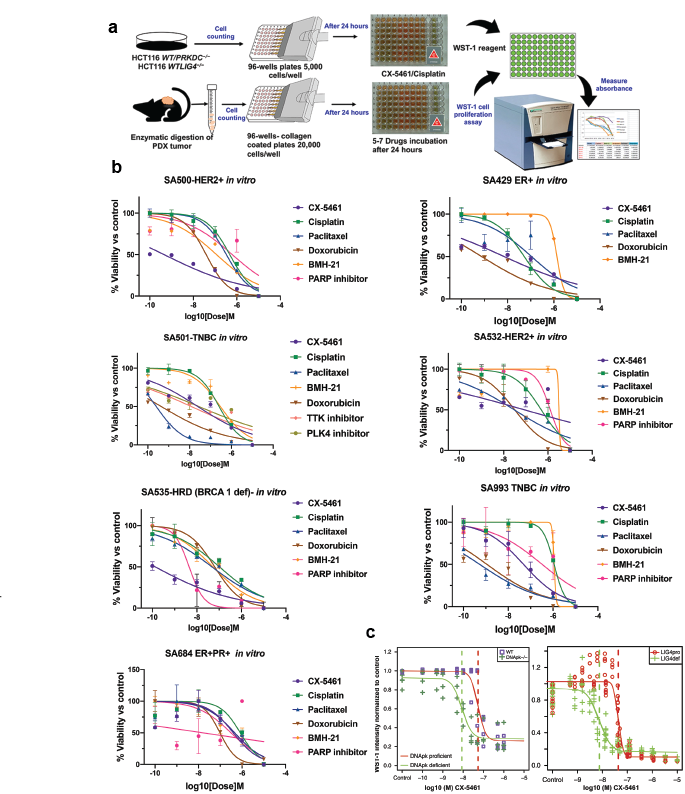
\includegraphics[width=\textwidth]{Figures/chap3/invitro.png}
	\caption[Representative graphs from drug efficacy testing \textit{in vitro} ]
	{\small
	    \textbf{Drug efficacy testing \textit{in vitro}.}
	    \textbf{(a)} Schematics of experimental design
	    \textbf{(b)} Response of PDX tumor cells to chemotherapies \textit{in vitro} (n=4). Each graph represent each type of PDX tumor tested with the drugs mentioned in its key. Vertical axis represents percent viability normalized to control. Horizontal axis present drug doses.
	   
	}
	\label{fig:invitro}
\end{figure}

%-----------------------------------------------------------------

 % Table generated by Excel2LaTeX from sheet 'Sheet1'
 \begin{table}[htbp]
   \centering
   \caption{Summary of logIC50 values of PDX responses \textit{in vitro}}
     \begin{tabular}{|c|p{5em}|c|c|c|c|c|r|r|}
        \hline
       & \multicolumn{7}{|c|}{\textbf{Patient derived xenografts}} \\
          \hline
       & \textbf{SA429} & \textbf{SA500} & \textbf{SA501} & \textbf{SA532} & \textbf{SA535} & \multicolumn{1}{|c|}{\textbf{SA684}} & \multicolumn{1}{|c|}{\textbf{SA993}}\\
     \multicolumn{1}{|l|}{\textbf{Drug (LogIC50)M}} & \textbf{(ER+)} & \textbf{(HER2+)} & \textbf{(TNBC)} & \textbf{(HER2+)} & \textbf{(TNBC-HRD)} & \multicolumn{1}{|c|}{\textbf{(ER+)}} & \multicolumn{1}{|c|}{\textbf{(TNBC)}} \\
        \hline
     CX-5461  & -8.149 & -9.345 & -7.607 & -7.058 & -9.876 & -6.403 & -7.316 \\
     Cisplatin  & -7.28 & -6.324 & -7.680 & -6.302 & -6.987 & -6.08 & -5.954 \\
     Paclitaxel  & -6.965 & -6.48 & -9.6 & -7.519 & -8.324 & -6.338 & -9.274 \\
     Doxorubicin  & -9.122 & -7.238 & -9.361 & -7.498 & -7.2 & -7.014 & -8.951 \\
     BMH-21  & -5.866 & -6.932 & -6.527 & -5.502 & -7.281 & -6.508 & -5.951 \\
     Pyridostatin & -6.302 & N/A & N/A & N/A & -6.698 & -6.687 & -6.321 \\
     PARP inhibitor  & N/A & -6.208 & N/A & -5.894 & -8.348 & -7.798 & -6.484 \\
     Docetaxel  & N/A & -6.202 & -12.88 & N/A & -8.175 & -5.718 & -8.674 \\
     Fluorouracil (5-FU)  & N/A & -6.467 & -5.999 & N/A & -6.374 & -6.664 & -6.357 \\
     Carboplatin  & N/A & -5.946 & N/A & N/A & -6.373 & -6.583 & -6.009 \\
     Methotrexate  & N/A & -7.576 & -7.203 & N/A & -7.589 & -6.088 & -7.794 \\
    
     \hline
     \end{tabular}%
   \label{tab:invitroIC50}%
   
   
    \small\textbf{ (N/A: not applicable)}.
 \end{table}%

%%%%%%%%%%%%%%%%%%%%%%%%%%%%%%%%%%%%%%%%%%%
\begin{figure}
\centering
	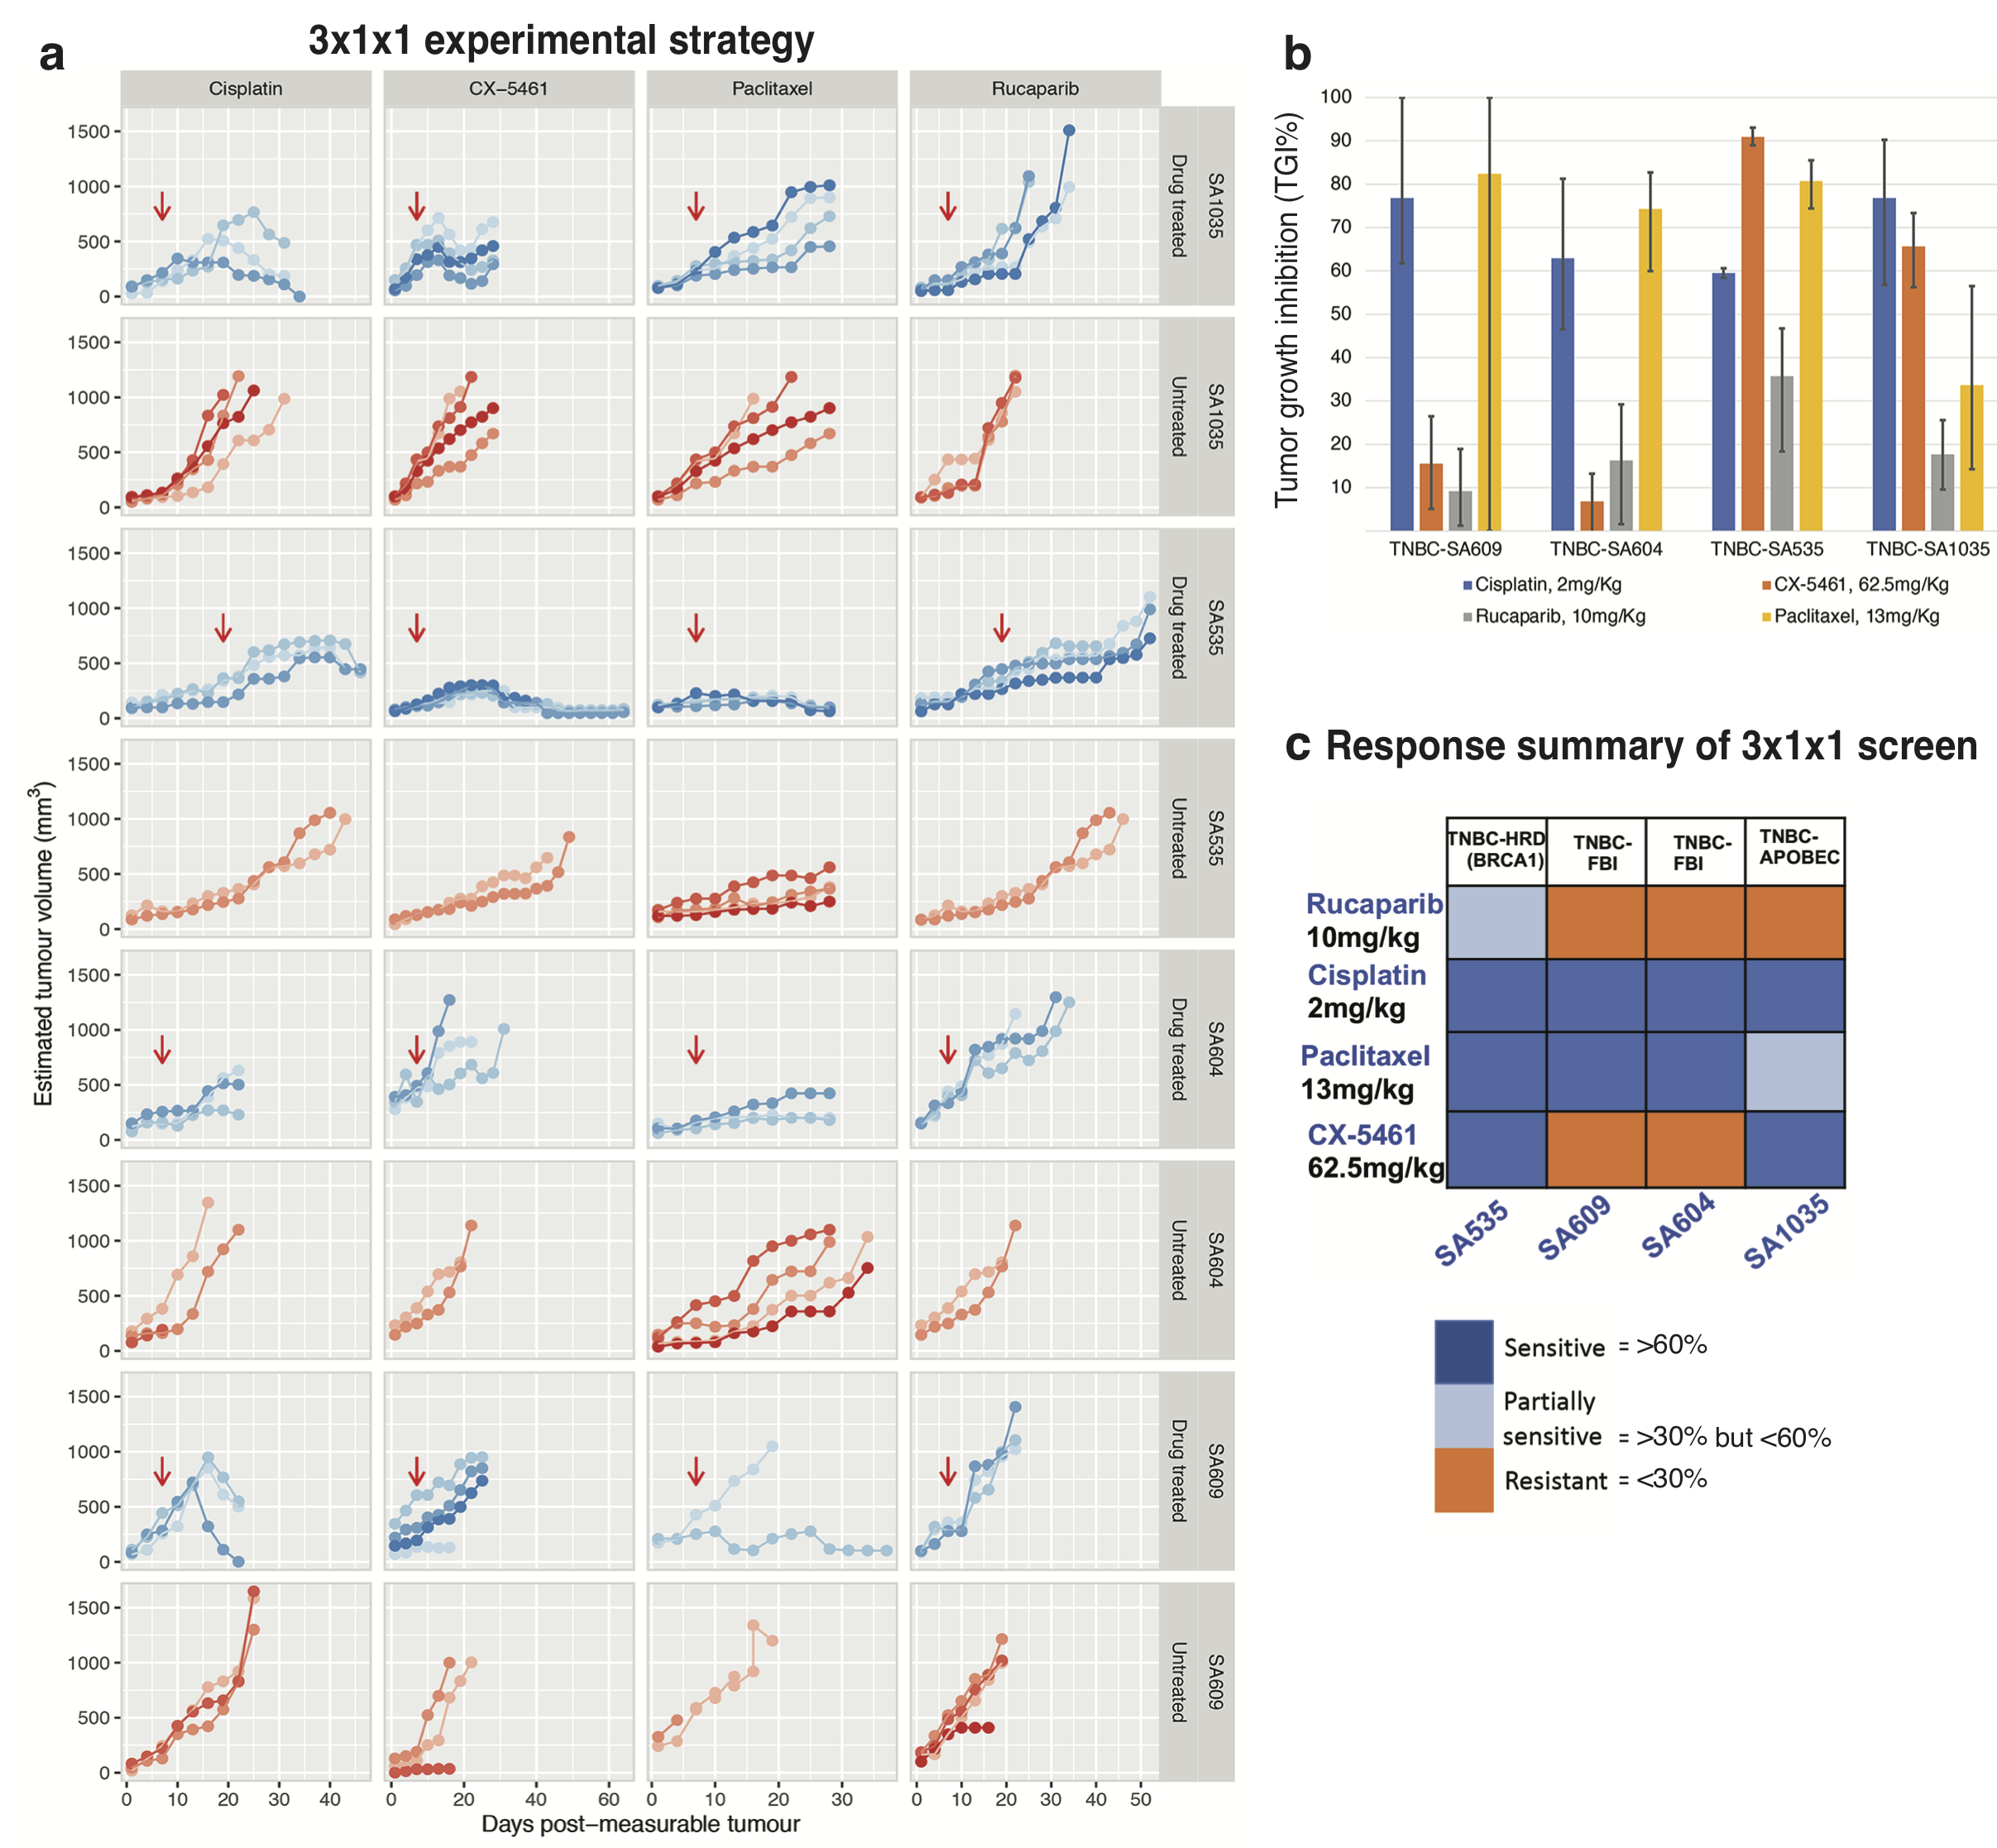
\includegraphics[width=\textwidth]{Figures/chap3/4drugs4PDXNew.png}
	\caption[Representative tumor responses from four PDX and  to four drugs]
	{\small
	   \textbf{Representative tumor responses from four PDX and  to four drugs.}
	    \textbf{(a)} Summary matrix of four TNBC PDX with drugs
	     \textbf{(b)} Bar plot showing tumor growth inhibition percentages. Error bars represent one standard deviation based on 2-4 replicate tumor growth inhibitions.
	    \textbf{(c)} Tumor growth curves from treated and un treated tumors. Vertical axis representing the tumor volume in cubic millimeters and horizontal axis is showing the days tumor measurements. Red arrows represent the time of start of treatments.
}
	\label{fig:EstablishmentofPDX}
\end{figure}

%%%%%%%%%%%%%%%%%%%%%%%%%%%%%%%%%%%%%%%%%%%


% Table generated by Excel2LaTeX from sheet 'table for R'
\begin{table}[htbp]
  \centering
  \caption{Summary responses \textit{in vivo} with 3x1x1 strategy trichotomized tumour response based on TGI \cite{hather2014growth, aykan2020objective}}
    \begin{tabular}{|l|l|l|l|l|}
    
     \hline
    \textbf{Tumor ID} & \textbf{Cisplatin} & \textbf{Paclitaxel} & \textbf{Rucaparib} & \textbf{CX-5461} \\
     \hline
    HER2+SA532 & N/A   & N/A   & N/A   & Sensitive \\
    TNBC-SA535 & Sensitive & Sensitive & Partially-Sensitive & Sensitive \\
    TNBC-SA605 & Sensitive & Sensitive & N/A   & N/A \\
    TNBC-SA604 & Sensitive & Sensitive & Resistant & Resistant \\
    TNBC-SA609 & Sensitive & Sensitive & Resistant & Resistant \\
    TNBC-SA919 & N/A   & Sensitive & N/A   & N/A \\
    HER2-SA920 & N/A   & N/A   & N/A   & Resistant \\
    TNBC-SA993 & N/A   & N/A   & N/A   & Sensitive \\
    ER+SA995 & N/A   & N/A   & N/A   & Partially-Sensitive \\
    TNBC-SA1035 & Sensitive & Partially-Sensitive & Resistant & Sensitive \\
    TNBC-SA1130 & Sensitive & N/A   & N/A   & Sensitive \\
    TNBC-X2371 & Sensitive & Partially-Sensitive & N/A   & Sensitive \\
    TNBC-X2440 & Sensitive & Sensitive & N/A   & N/A \\
     \hline
    \end{tabular}%

\small\textbf{PDX ID = Patient-derived xenograft identification, N/A = not applicable}\\
  \label{tab:PDXtumorsinvivo}%


   \small\textbf{ (Tumor growth inhibition (TGI): Sensitive= $>$60\%; Partially-Sensitive= $>$30\% but $<$60\%; Resistant= $<$30\%)}.
\end{table}%

%%%%%%%%%%%%%%%%%%%%%%%%%%%%%%%%%%%%%%%%%%%



%--------------------------------------------

\subsection{Baseline \textit{in vivo} sensitivity patterns of triple negative breast cancer}
To evaluate the spectrum of baseline sensitivity of PDX tumors with conventional and novel targeted chemotherapies, we modified the previously published 1x1x1 design for semi-quantitative PDX drug senstivity mapping, increasing the number of replicate mice to a 3x1x1 design. \cite{gao2015high,migliardi2012inhibition}. 
%We performed \textit{in vivo} screen to model inter-patient response heterogeneity with \textbf{three animals per model per treatment strategy (3x1x1)}. 
 13 PDXs were tested with cisplatin, Paclitaxel, Rucaparib or CX-5461. NOtably, all 8 of the TNBC tested were sensitive to cisplatin with tumor growth inhibition of more than 60\%, however, less responsive to Rucaparib \textbf{Summary in \autoref{tab:PDXtumorsinvivo}}. 
We selected in total of four drugs, including two standard chemotherapies, platinum (cisplatin-(2mg/kg, \ac{Q3Dx8}, \ac{IP} max)) and Taxanes (Paclitaxel-13mg/kg, \ac{Q3Dx8}, \ac{IP} max), and two targeted chemotherapies, PARP inhibitors (Rucaparib-\ac{IP} daily 5 days per week for 3 weeks) and G4 quadruplex stabilizers (CX-5461-62.5mg/kg, \ac{Q3Dx8} by oral gavage). 
\textbf{\autoref{fig:EstablishmentofPDX} a} showing summary matrix of four triple negative breast (TNBC) PDX towards chemotherapies. 
The representative growth curves are shown in \textbf{\autoref{fig:EstablishmentofPDX} c}, including TNBC-SA609 (Basal, TP53, FBI), TNBC-SA1035 (Basal, HRD, APOBEC-like, POLH), TNBC-SA535 (Basal, MMRD-1, S-Dup, TP53, BRCA1 def) and TNBC-SA604 (Basal, CI-SV, CI-FBI).

To classify tumor responses, we measured tumor growth inhibition percent (TGI\%) in each PDX and divided them into three categories according to modified RECIST criteria \cite{aykan2020objective}. Sensitive: \ac{TGI} $>$60\%; partially sensitive: \ac{TGI} $>$30\% but $<$60\%; Resistant: \ac{TGI} $<$30\% \textbf{\autoref{fig:EstablishmentofPDX} a}.
Interestingly, we found that all TNBC PDXs with different background mutational signatures behaved differently towards the same drugs. Both PDXs with FBI backgrounds, TNBC-SA609 and TNBC-SA604 were both found to be resistant to CX-5461 with tumor growth inhibition (TGI) of 15\% and 7\%, respectively \textbf{\autoref{fig:EstablishmentofPDX} b}. Moreover, they were resistant to Rucaparib as well, with \ac{TGI} of 9\% and 16\%, respectively.
All four of the PDX showed high sensitivity to platinum (cisplatin). Three out of four PDXs were sensitive to (taxane) paclitaxel, while TNBC-SA1035 was partially sensitive with \ac{TGI} of 34\%. Surprisingly,  TNBC-SA535 with BRCA deficiency was expected to be very sensitive to Rucaparib, but in our screening, it tend to be partially sensitive with \ac{TGI} of 36\% \textbf{\autoref{fig:EstablishmentofPDX} b}.


\section{Optimization methods in tumor dissociation for single cell analysis}

This section of chapter 3 belongs to \textit{Genome Biology, 2019} paper, title  \textbf{``Dissociation of solid tumor tissues with cold active protease for single-cell RNA-seq minimizes conserved collagenase-associated stress responses''}.
%%%%%%%%%%%%%%%%%%%%%%%%%%%%%%%%%%%%%%%%%%%%%%%%%%%%%%%%%%%%%%%%%%%%%%

\begin{figure}
	\centering
	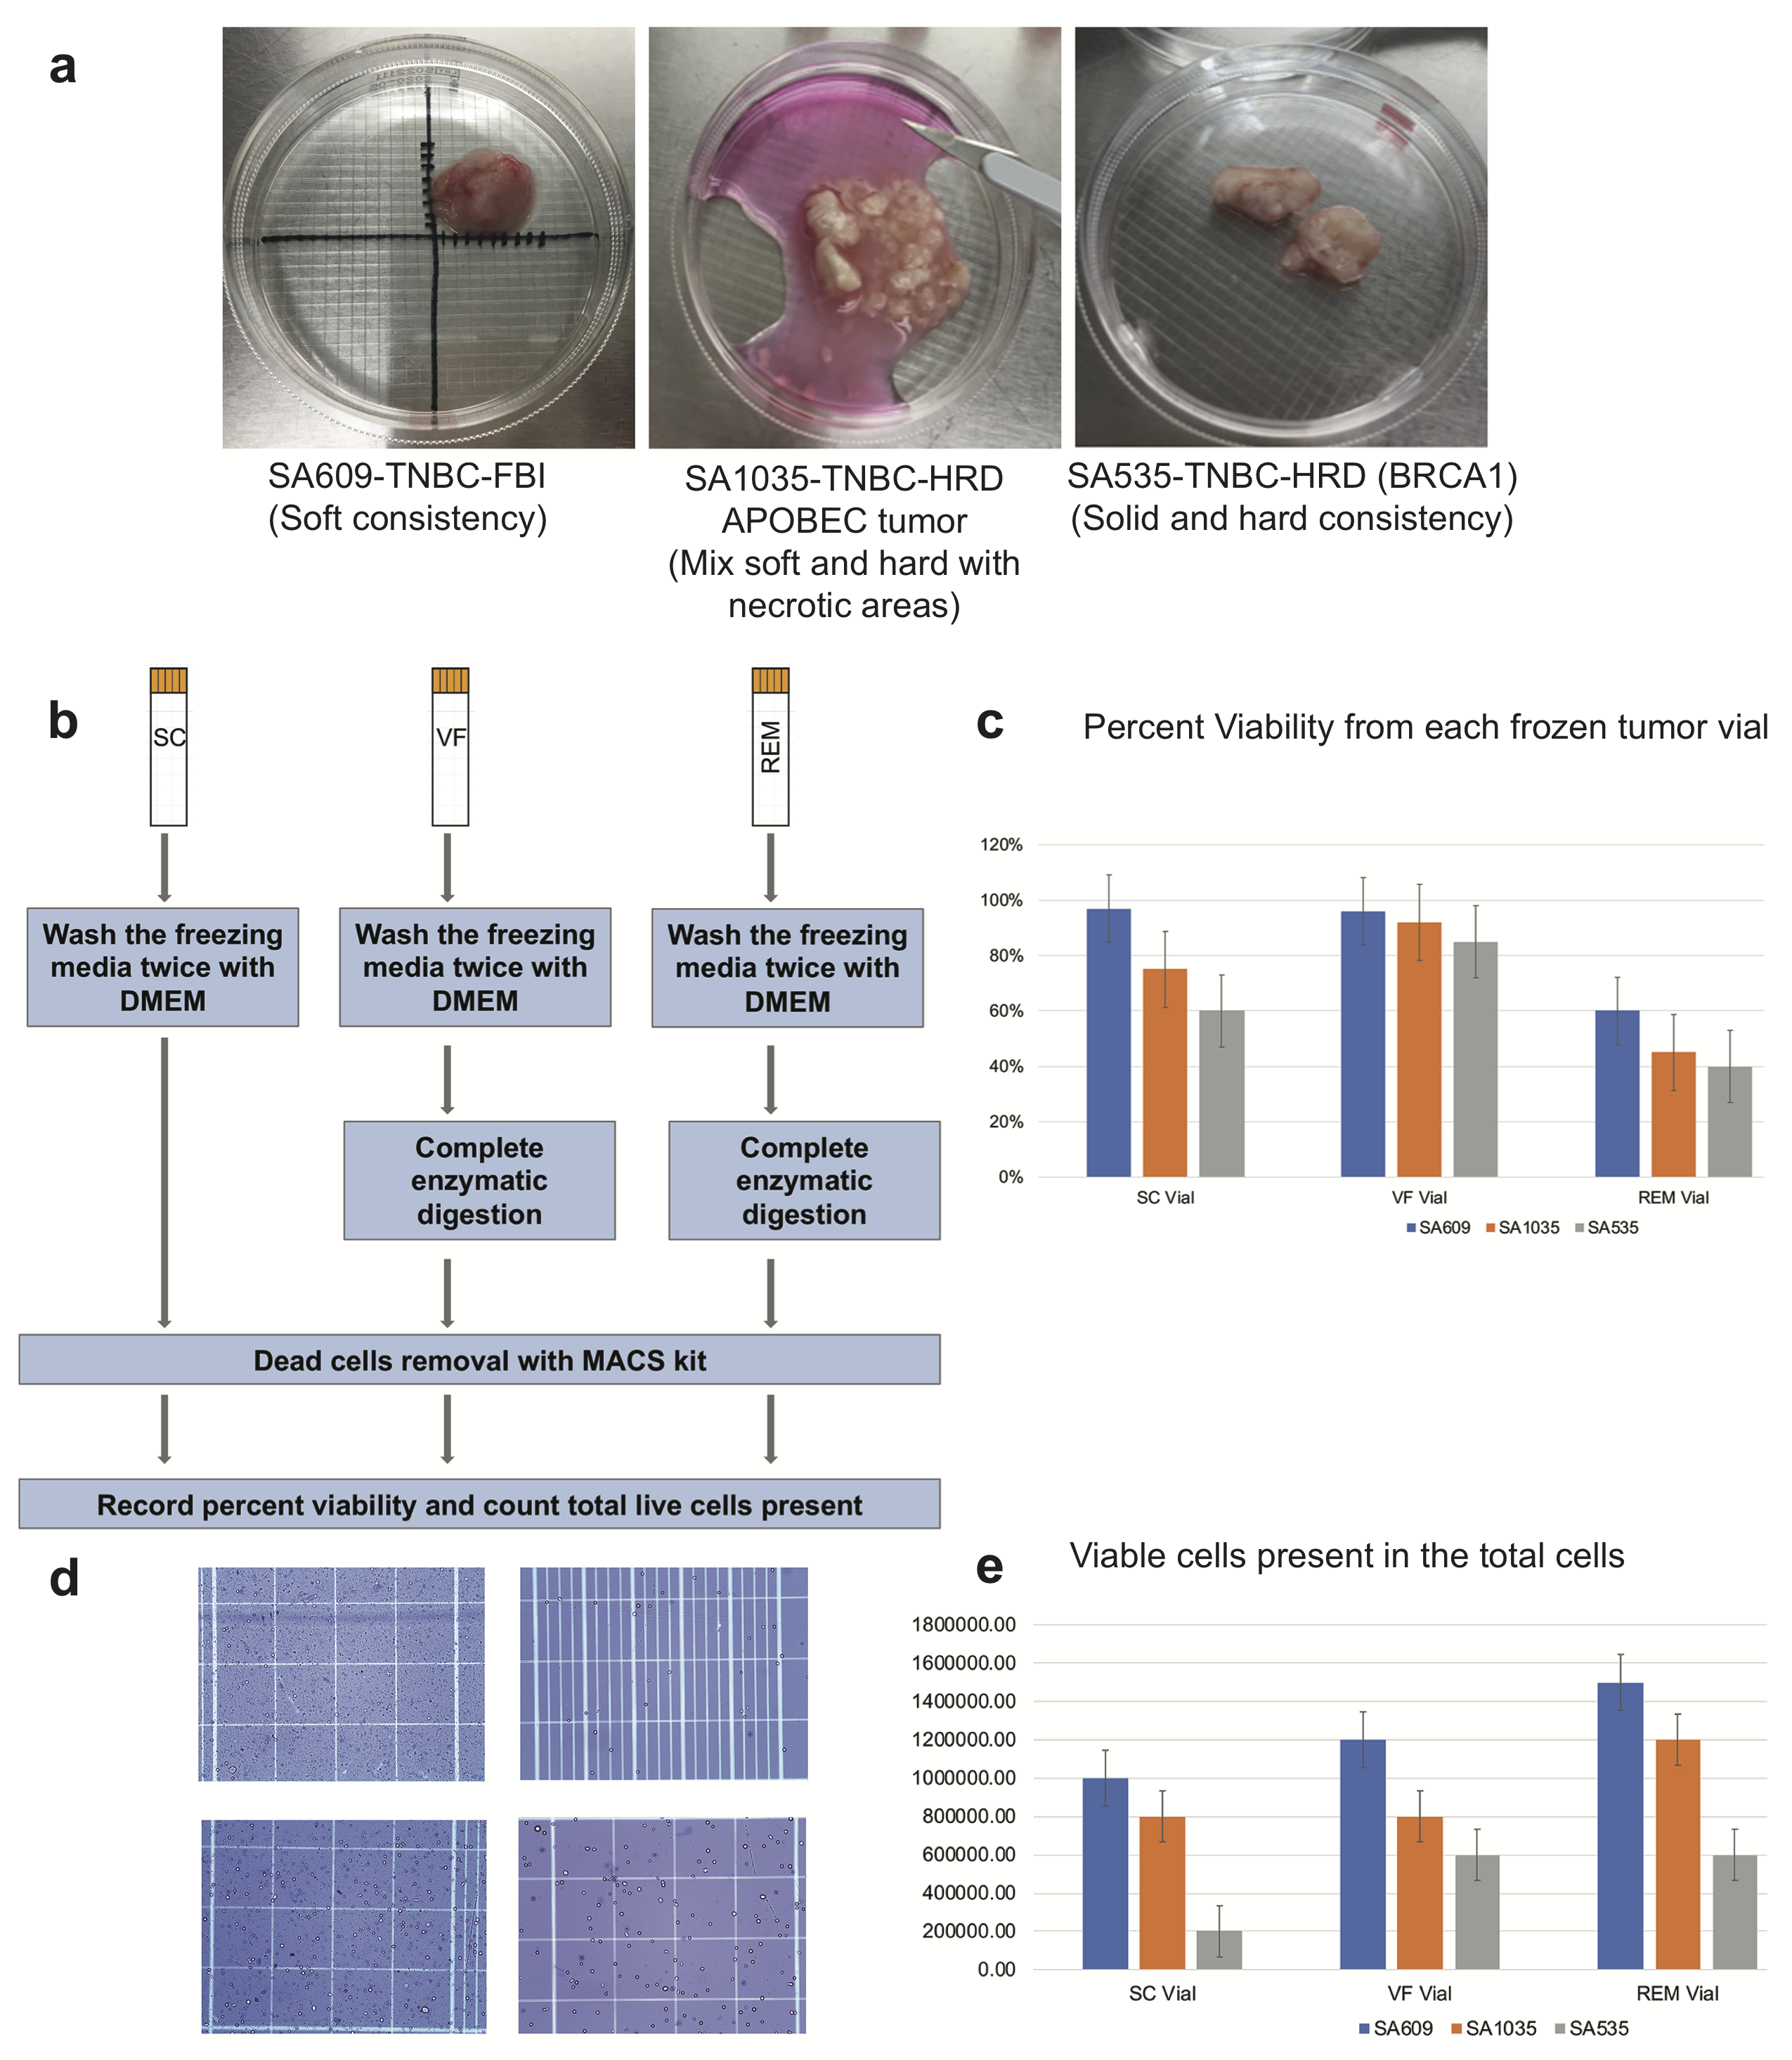
\includegraphics[width=\textwidth]{Figures/chap3/cellviability2.png}
	\caption[Evaluation of viable-high percent cell recovery for single cell measurements]
	{\small
	    \textbf{Evaluation of viable-high percent cell recovery for single cell measurements.}
	    \textbf{(a)} Representative tumors in dishes. Two small black lines as 2mm. Middle dish showing partially chopped tumor with white necrotic tissues. Right side panel showing example from comparatively solid to cut tumor.
	    \textbf{(b)} Schematics of processing the frozen vials.
	    \textbf{(c)} Vertical axis showing the percent viability and horizontal axis shows the type of vials from each of three tumors  \textbf{(d)} Left sided images are pre-dead cell removal while right sided are the post dead removal \textbf{(e)} Vertical axis showing the number of viable cells obtained from each vial and horizontal axis shows type of vials processed.
	}
	\label{fig:cellviability}
\end{figure}
%%%%%%%%%%%%%%%%%%%%%%%%%%%%%%%%%%%%%%%%%%%%%%%%%%%%%%%%%%%%%%%%%%%%%%


\subsection{Small viable frozen fragments of the tumors culminated in high viability and less debris as compared to big frozen chunks}
To investigate which status of tissue freezing will give us better outcome of single cell suspension, we mechanically disaggregated three TNBC PDX tumors \textbf{\autoref{fig:cellviability} a}, TNBC-SA609, TNBC-SA1035 and -TNBC-SA535 and froze them in three different ways. First, after mechanical digestion, viable frozen (VF) tissue fragments were frozen in the freezing media. Second, consist of single cells (SC) by complete enzymatic digestion \textbf{(See methods)} and lastly big tissue chunks frozen vial labelled as ``REM'' (remaining). 
Tumor fragments were thawed and washed twice with 
Gibco Dulbecco's Modified Eagle Medium (DMEM) media. VF and REM fragments were digested to single cells with collagenase hyaluronidase and dead cells and debris were removed from all the single cells final suspension as described in the method section \textbf{\autoref{fig:cellviability} b}. We obtained high percent viabilty from viable frozen tumor fragments across all the three tested PDX tumors ranging approximately from 82\% to 95\% as compared to big chunks (REM) or SC cells \textbf{\autoref{fig:cellviability} c}.
However, the final number of viable cells in each of the condition across different PDX varies from 200 thousands to one million cells \textbf{\autoref{fig:cellviability} e}. Interestingly, one of the PDX tumor, SA609-TNBC turns out to be behaving comparatively effectively under every condition. 
Finally, in order to  remain consistent across every type of tumor, we concluded that Viable frozen "VF" is the best option giving us moderate number of viable cells across xenografts.
Also, we found that dead cell removal step helped cleaning up debris providing high percentage of viable cells \textbf{\autoref{fig:cellviability} d}.


%----------------------------------------------------------------


%--------------------------------------------------------------------

\subsection{Dissociation with Collagenase at 37\textdegree C induces a distinct stress response in single-cell transcriptomes}
To uncover transcriptional variation and responses to dissociation method and to see the effect of digestion temperature on the transcriptome, we generated scRNA-seq data from a range of PDX tumors dissociated at low temperature with cold active protease and at high temperature with collagenase and Hyaluronidase, using the 10x Genomics Chromium v3 platform \textbf{(see methods)}.
We performed a differential expression analysis on the 23,731 cells found by combining all experiments measured in PDX tumors at either 6\textdegree C or 37\textdegree C. After retaining genes with at least 10 counts across all cells, we performed differential expression analysis with edgeR \cite{robinson2010edger}, while controlling for the sample-of-origin.
We found that of the 19,464 genes retained for analysis, 11,975 (62\%) were differentially expressed at a Benjamini-Hochberg corrected false discovery rate (FDR) of 5\%. We defined a core set of genes meaningfully perturbed by digestion temperature as those significantly differentially expressed as above, but with an absolute log fold change of at least 1.5. Therefore, for a gene to be included under these criteria it must be differentially expressed and its abundance increased or decreased by at least 50\% by digestion temperature. 

%-------------------------------------------------------------------------

\begin{figure}
	\centering
	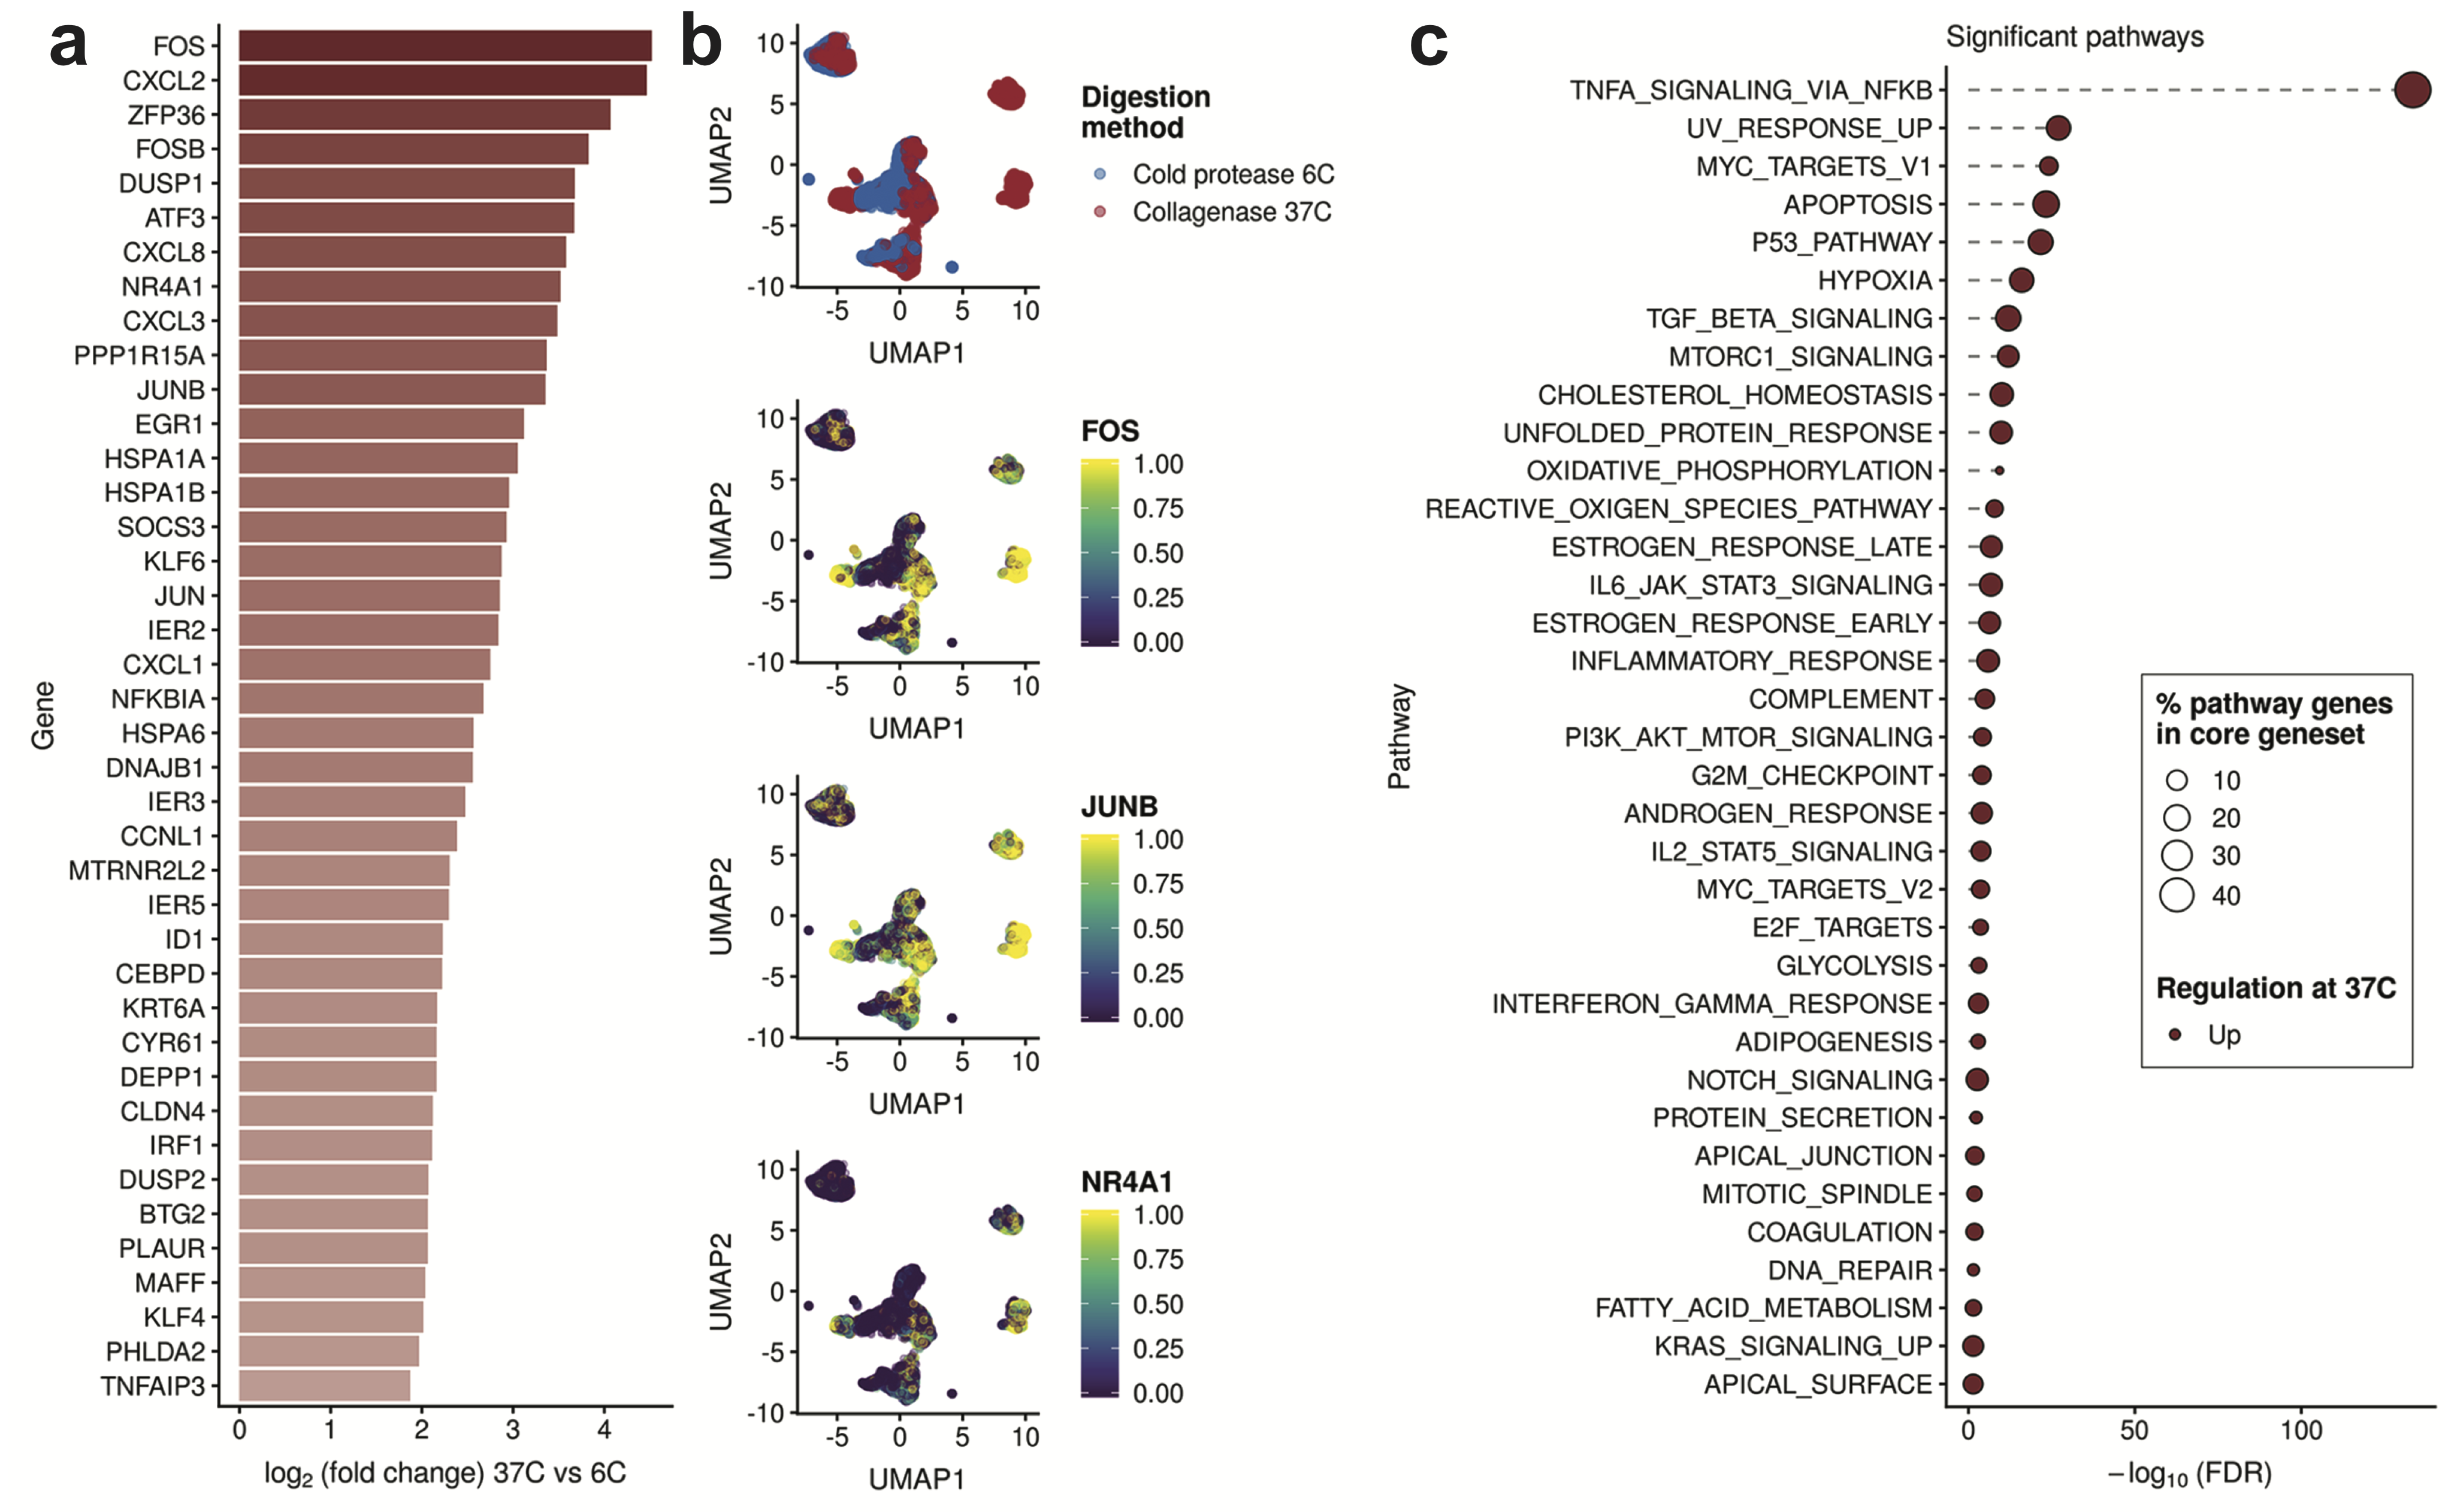
\includegraphics[width=\textwidth]{Figures/chap3/stressresponse1.png}
	\caption[Dissociation with collagenase induces a distinct stress response in PDX tumors]
	{\small
	    \textbf{Dissociation with collagenase induces a distinct stress response in PDX tumors.}
	    \textbf{(a)} The top 40 genes (by log fold-change) from the 11,975 identified as significantly differentially expressed between cells digested at 6\textdegree C and 37\textdegree C.
	    \textbf{(b)} UMAP plots of 23,731 cells coloured by digestion temperature (top) then by normalized expression of 3 key stress response genes (\textit{FOS}, \textit{JUNB}, \textit{NR4A1}) demonstrates a distinct concordance between temperature and induction of the stress gene signature.
    Expression values are log normalized counts winsorized to $[0,2)$ then scaled to $[0,1)$
	    \textbf{(c)} Pathway analysis of differentially expressed genes with the MSigDB hallmark gene sets highlights induction of genes involved in NF-$\kappa$B signalling at 37\textdegree C digestion with 46.5\% of 200 genes annotated in the pathway being found in the 512 core gene set}
	\label{fig:stressresponseinpdx}
\end{figure}

%-------------------------------------------------------------------------

This produced a core gene set of 512 genes, of which 507 were upregulated at 37\textdegree C and the remaining 5 downregulated. This gene set included multiple canonical stress-related genes such as \textit{FOS}, \textit{FOSB}, \textit{ATF3} and heat shock proteins (HSPs) \textbf{\autoref{fig:stressresponseinpdx} a}, expression of which had shown to be induced by collagenase dissociation in a subset of muscle cells \cite{van2017single}. A \ac{UMAP} embedding of the cells coloured by dissociation temperature and the expression of several key genes (\textit{FOS}, \textit{JUNB}, \textit{NR4A1}) \textbf{\autoref{fig:stressresponseinpdx} b}, further demonstrated the digestion temperature-specific induction of the expression of these genes.
We subsequently performed a pathway enrichment analysis on the differential expression results, searching for enrichment in given hallmark pathways \cite{liberzon2015molecular} \textbf{\autoref{fig:stressresponseinpdx} c}. Of particular note was TNF (tumor necrosis factor) signalling via NF-$\kappa$B of which 46.5\% of annotated pathway genes were included in the core set of 512 genes. Further enrichment of stress-associated pathways including hypoxia, apoptosis, and inflammatory response was further indicative of collagenase dissociation at 37\textdegree C as inducing a stress response on the transcriptomes of single cells.

 \subsection{Identification of subpopulations of dead, dying and live cells in transcriptomic data}
Given the bi- and tri-modal distributions of mitochondrial gene count percentages \cite{o2019dissociation} apparent in the PDX experiments and previous studies' assertions that high mitochondrial gene content is indicative of dead and dying cells \cite{ilicic2016classification, zhao2002mitochondrial}, we next sought to determine the contribution of dead and dying cells to the variation observed in QC metrics  \cite{o2019dissociation}. In order to induce classical cell death pathways, we used TNF\textalpha    
 \cite{carswell1975endotoxin, sedger2014tnf} to treat the non tumourigenic, lymphoblastoid cell line GM18507 and FACS sorted cells into dead or and dying fractions based on PI/Annexin V positivity \textbf{\autoref{fig:livedead} a)}, as well as a live, untreated fraction. Notably, cell yield from scRNAseq data was highly dependent on the cell status, with 8,597 live cells recovered but only 1,280 and 885 dead and dying, respectively, compared to targeted numbers of 3,000 cells. 
A principal components analysis (PCA) following mutual nearest neighbours (MNN) correction \cite{haghverdi2018batch} demonstrated the cells approximately segregating along the first principal component (PC1) by cell status \textbf{\autoref{fig:livedead} b)}, albeit with high levels of heterogeneity in overlap. Indeed, PC1 closely tracked the mitochondrial gene content of the cells \textbf{\autoref{fig:livedead} c)}, being significantly higher in dead cells (median 29.9\%) compared to both dying cells (median 3.13\%, $p=1.17 \mathrm{e}{-126}$) and live cells (median 3.4\%, $p=4.65 \mathrm{e}{-153}$) as shown in \textbf{\autoref{fig:livedead} d}.
This observation justifies the practice of excluding cells with very high mitochondrial gene content as being likely dead cells.

Conscious of the possibility of murine stromal cell contamination in PDX samples, we classified cells as mouse or human based on alignment metrics. Of the 99,244 PDX cells sequenced, 4942 were reliably identified as mouse cells, with large inter-sample variation \textbf{\autoref{fig:mouseqc}}.
As expected, murine cells scored consistently lower across a range of standard QC metrics (percentage of mitochondrial counts, total genes detected, total \ac{UMIs} detected) when aligned to the human genome \textbf{(see methods)}.
%-----------------------------------------------------------

\begin{figure}
\centering
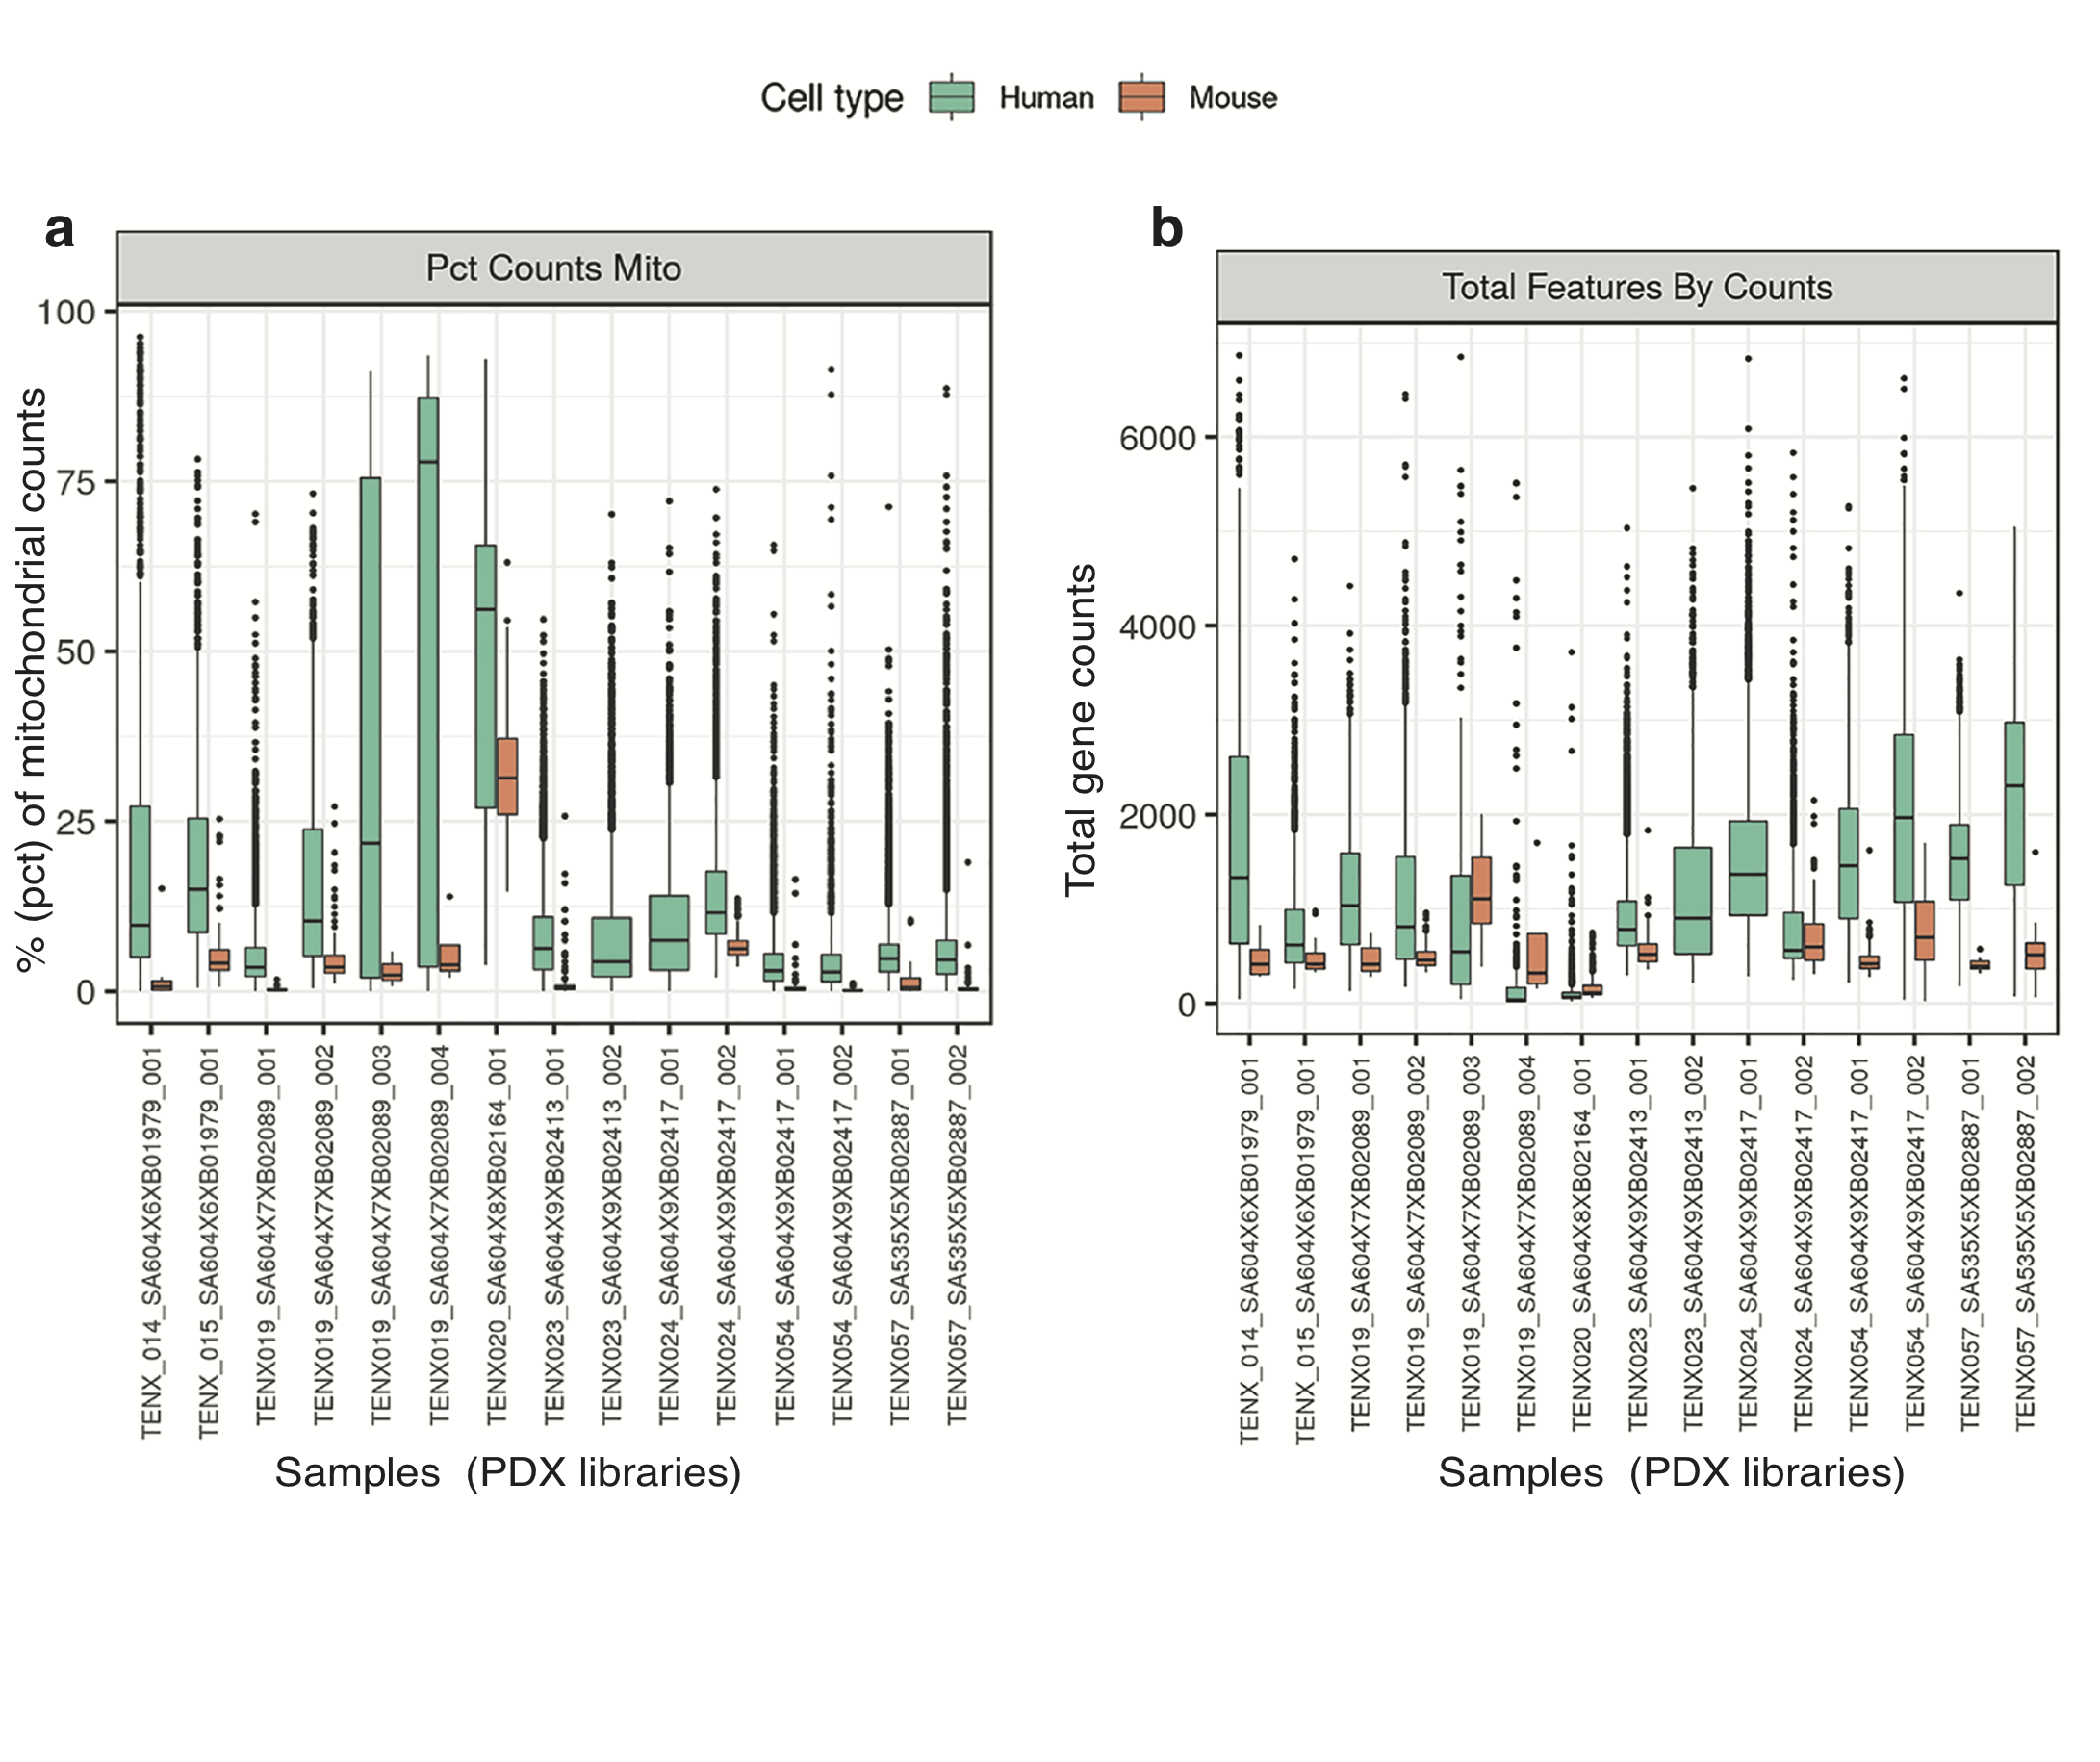
\includegraphics[width=\textwidth]{Figures/chap3/mouseqc.png}
	
\caption[Quality control metrics (\% mitochondrial gene counts, total counts, total genes detected)]
	{\small
	\textbf{Quality control metrics (\% mitochondrial gene counts, total genes detected).}
	 All scRNA-seq of PDX included in the study, on average, of murine cells score lower across all three metrics though with notable inter-dataset variability.
	   \textbf{(a)} Vertical axis represents the percentage of mitochondrial genes detected in mouse or human samples. Horizontal axis denotes the sample IDs from each of the PDX library. 
	  \textbf{(b)} Vertical axis represents the total features (genes) of  genes detected in mouse or human samples. Horizontal axis denotes the sample IDs from each of the PDX library. 
	}
	\label{fig:mouseqc}
\end{figure}

%-----------------------------------------------------------------------
\begin{figure}
	\centering
	\includegraphics[width=\textwidth]{Figures/chap3/livedead.png}
	\caption[Transcriptomic landscape of live, dead, and dying cells.]
	{\small
	    \textbf{Transcriptomic landscape of live, dead, and dying cells.}
	    \textbf{(a)} FACS analysis showing gating strategy for untreated, live cells (PI$-$/annexin V$-$) or TNF\textalpha-treated dying cells (PI/annexin V+) and dead cells (PI+/annexin V+).
	    \textbf{(b)} PCA projection of the three cell conditions showing approximate segregation of cell status along the first principal component (PC1), with live and dying cells enriched at lower PC1 values and dead cells enriched at higher values.
	    \textbf{(c)} PCA projection colored by the percentage mitochondrial genes (``\% transcriptome mitochondrial'') shows significant increase along the PC1 \textbf{(d)} Dead cells exhibit significantly higher percentage of the transcriptome as mitochondrial compared to both live and dying cells \textbf{(e)} Unsupervised clustering of the gene expression profiles clusters the cells into three groups, approximately tracking both PC1 of the data and the percentage of transcriptome mitochondrial \textbf{(f)} The composition of each cluster demonstrates that cluster 1 is primarily composed of live cells, cluster 2 a mix of live, dying, and dead cells, while cluster 3 is composed mainly of dead cells \textbf{(g)} The\% transcripts mitochondrial is significantly different between the three clusters, with a step increase in proportion moving from cluster 1 to 2 and 2 to 3 \textbf{(h)} Cluster 2 significantly up-regulates the MHC class I gene set, suggesting it represents stressed or pre-apoptotic cells.
	}
	\label{fig:livedead}
\end{figure}

%-------------------------------------------------------------------------

\begin{figure}
	\centering
	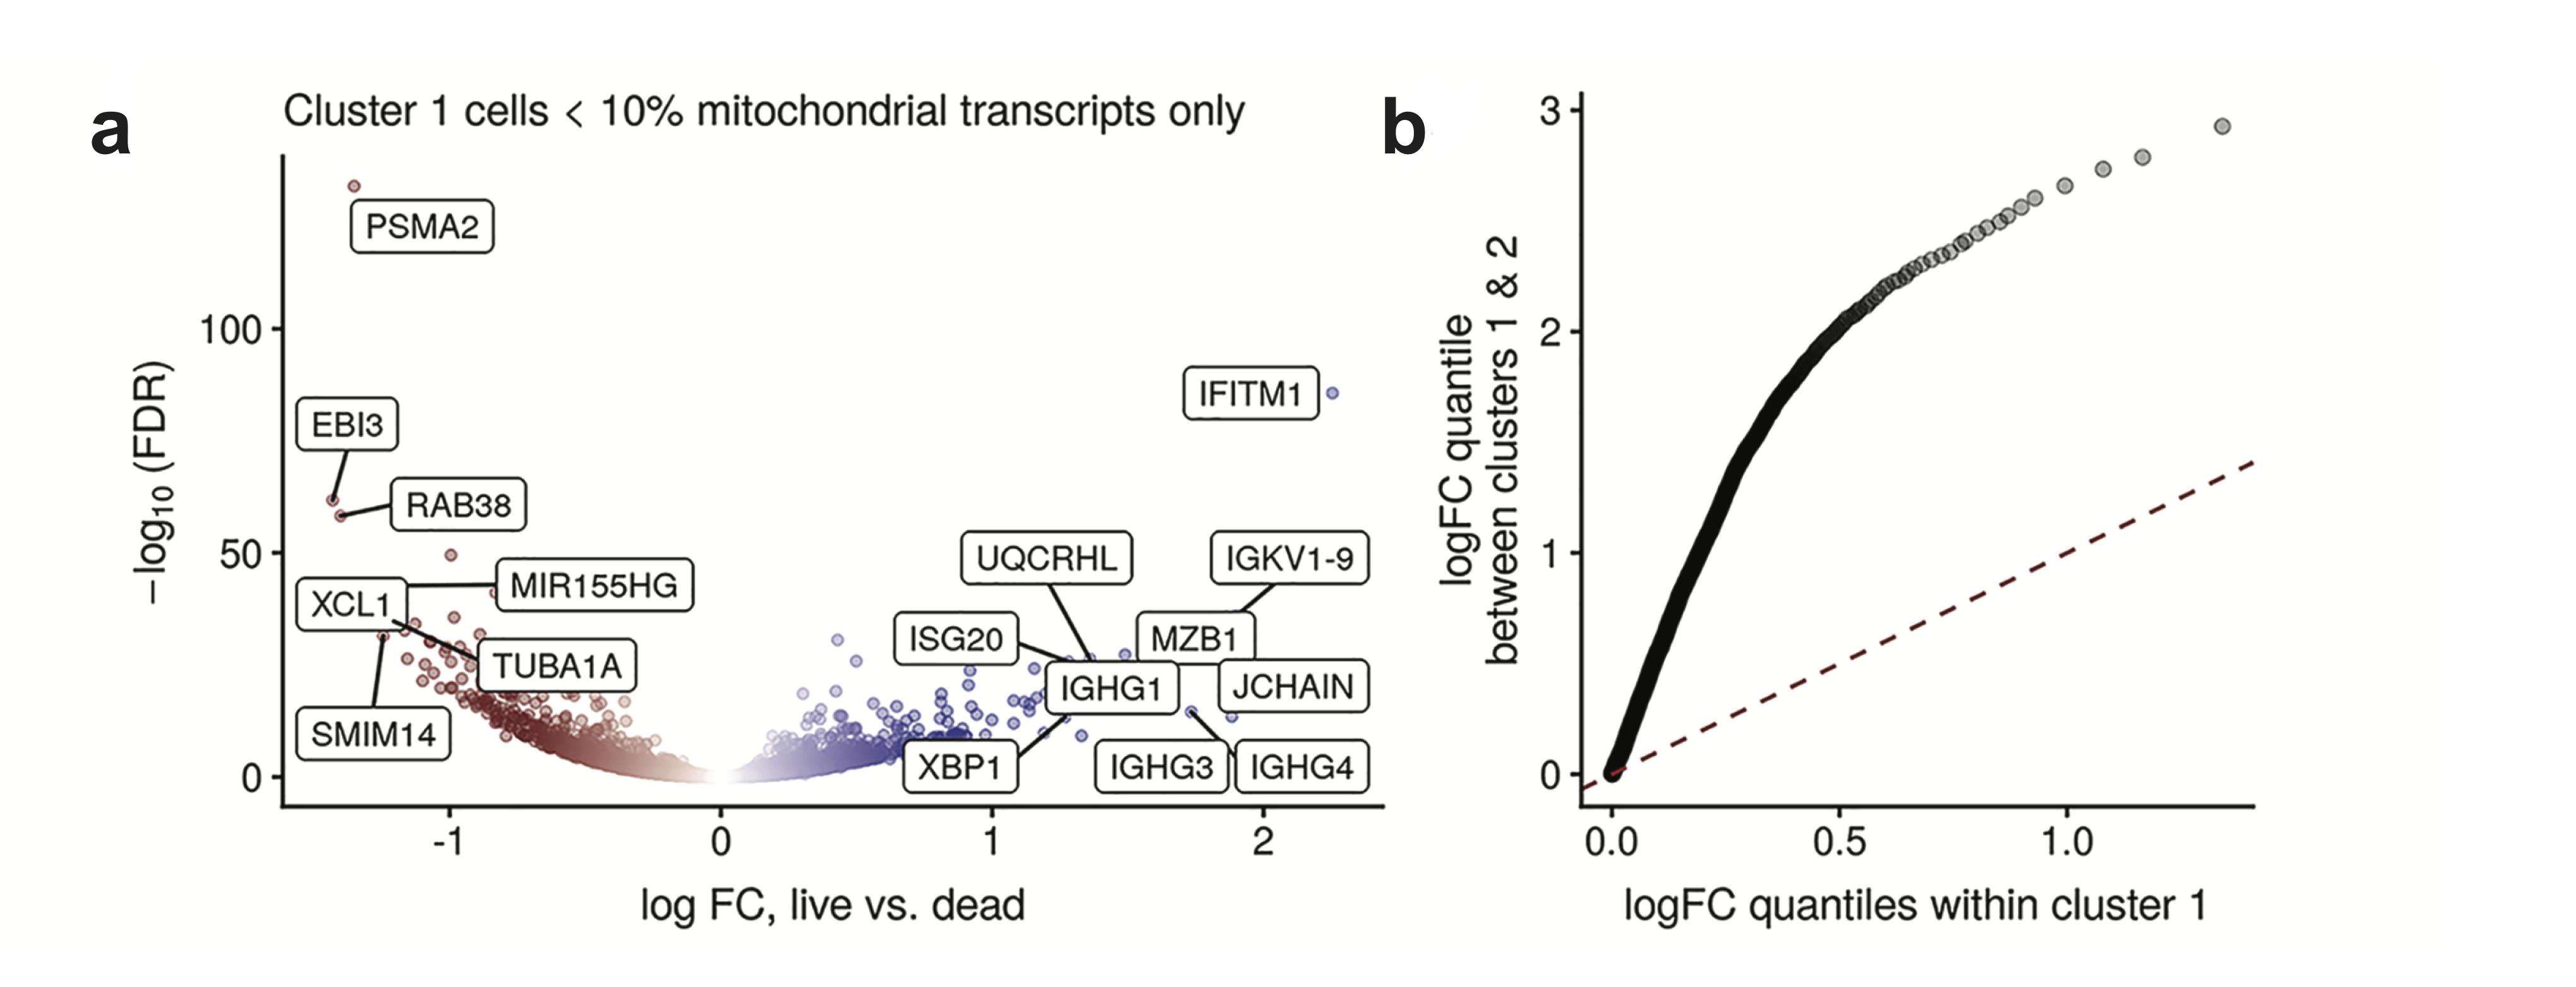
\includegraphics[width=\textwidth]{Figures/chap3/livedead2.png}
	\caption[Differential expression of cluster 1 of live, dead, and dying cells.]
	{\small
	 \textbf{Differential expression of cluster 1 of live, dead, and dying cells.}
    \textbf{a} Differential expression analysis of transcriptomically ``healthy'' cells within cluster 1 reveals residual differences between cells sorted as live and dead.
    \textbf{b} The distribution of absolute effect sizes (log fold change) of live vs. dead cells within cluster 1 (x-axis) compared to between clusters 1 and 2 (y-axis) demonstrates the residual effect on the transcriptome of being live/dead sorted is small compared to the inter-cluster expression variance.}
	\label{fig:livedead2}

\end{figure}
%-----------------------------------------------------------

Having observed that the transcriptomes of the different cell conditions are not entirely distinct, we sought to discover the extent of mixing between transcriptomic states and whether live and dead cells that appear transcriptomically ``healthy'' (i.e would ordinarily pass QC) are distinguishable. Using hierarchical clustering \textbf{(see methods)}, we clustered the cells into 3 groups  that approximately track PC1  \textbf{\autoref{fig:livedead} e)}. Interestingly, these three groups show variable composition in terms of cell states, with cluster 1 being comprised mainly of live cells 86\% live, 8.5\% dying, 5.1\% dead), cluster 2 containing an increased proportion of dying and dead cells (68\% live, 7.5\% dying, 24\% dead), and cluster 3 comprised mainly of dead cells (5.9\% live, 6.7\% dying, 87\% dead). This clearly demonstrates that cluster 1 is primarily composed of live cells and cluster 2 a mix of live, dying, and dead cells, while cluster 3 is composed mainly of dead cells, \textbf{\autoref{fig:livedead} f)}. Furthermore, we observed a step change increase in mitochondrial gene content between clusters \textbf{\autoref{fig:livedead} g)}, with cluster 1 having the lowest (median 3.13\%), followed by cluster 2 having a significant increase (median  26\%, $p=$ 0) and cluster 3 having a significant increase beyond that (median 82.2\%, $p=2.35\mathrm{e}{-149}$). 

Differential expression analysis between these clusters revealed a significant up-regulation in stress-associated pathways such as MHC class I,  \textbf{\autoref{fig:livedead} h)} in cluster 2 compared to clusters 1 \& 3. MHC class I genes are involved in antigen presentation to T cells, but are also expressed in many cell types and are induced in response to stress stimuli and contain heat shock-inducible elements \cite{gleimer2003stress}. 

Together, these results suggest a model whereby cluster 1 represents transcriptomically ``healthy'' cells, cluster 2 represents transcriptomically stressed cells that upregulate stress pathways  and have increased mitochondrial gene content (due to either an increasingly permeable membrane causing loss of cytoplasmic mRNA or increased metabolic demands), and cluster 3 represents transcriptomically dead cells whereby the membrane has burst leaving majority mitochondrial transcripts. Importantly, cells that are FACS sorted as either live, dying, or dead, are present in all three clusters, highlighting that the transcriptomic state of the cell is not necessarily the same as the surface marker state (though the two are correlated). Such concepts are reminiscent of ``pseudotime'' in single-cell developmental biology, whereby developmentally ordering cells transcriptomically can lead to early or late cells being placed at variable positions along the pseudotime trajectory \cite{campbell2018descriptive,campbell2018uncovering}. Indeed, PC1 from \textbf{\autoref{fig:livedead} a} approximates a pseudotime trajectory through the data, that tracks transcriptomically healthy cells to transcriptomically dead cells with increasing PC1 values.

\subsection{Live sorted and dead cells exhibit gene expression differences}
Next, we sought to determine if a sorted dead cell that appears transcriptomically healthy remains distinguishable from a sorted live cell in the transcriptomically healthy group. Using only cells in cluster 1, we further subsetted them to pass a strict set of QC filters (at least $10^3$ total genes detectable, \% mitochondrial content between 1 and 10) and performed a differential expression analysis between cells sorted as live and dead in this group. Of the 10,537 genes retained for analysis, 2,130 (20.2\%) were found to be differentially expressed \textbf{\autoref{fig:livedead2} a}, including downregulation of \textit{IFITM1} in dead cells. To compare this type of variation to the inter-cluster transcriptomic variation, we performed a second differential expression analysis between clusters 1 and 2, finding 8835 of 10,933 (80.8\%) genes significantly differentially expressed. Furthermore, the effect sizes were significantly larger for the inter-cluster comparison than the within-cluster 1 live-dead comparison as demonstrated by the quantile-quantile plot of absolute effect sizes in the \textbf{\autoref{fig:livedead2} b}. Collectively, these results suggest that though there are gene expression differences between dead and live sorted cells within cluster 1, the magnitude of expression variation is small compared to transcriptomically stressed clusters.
 
\subsection{Transcriptomic stress response is induced by both digestion time and digestion temperature}
To determine whether the gene signature identified above was induced due to the longer digestion time required for complete collagenase dissociation or due to the enzyme itself, we conducted a time course experiment, incubating breast PDX tissue with collagenase or cold protease for up to 3 hours. Since proteases work at different speeds on intact tissues, single cells released into the supernatant were sampled at 30 minutes, 1 hour, 2 hours or 3 hours.   

%------------------------------------------------------------------------- 

\begin{figure}
	\centering
	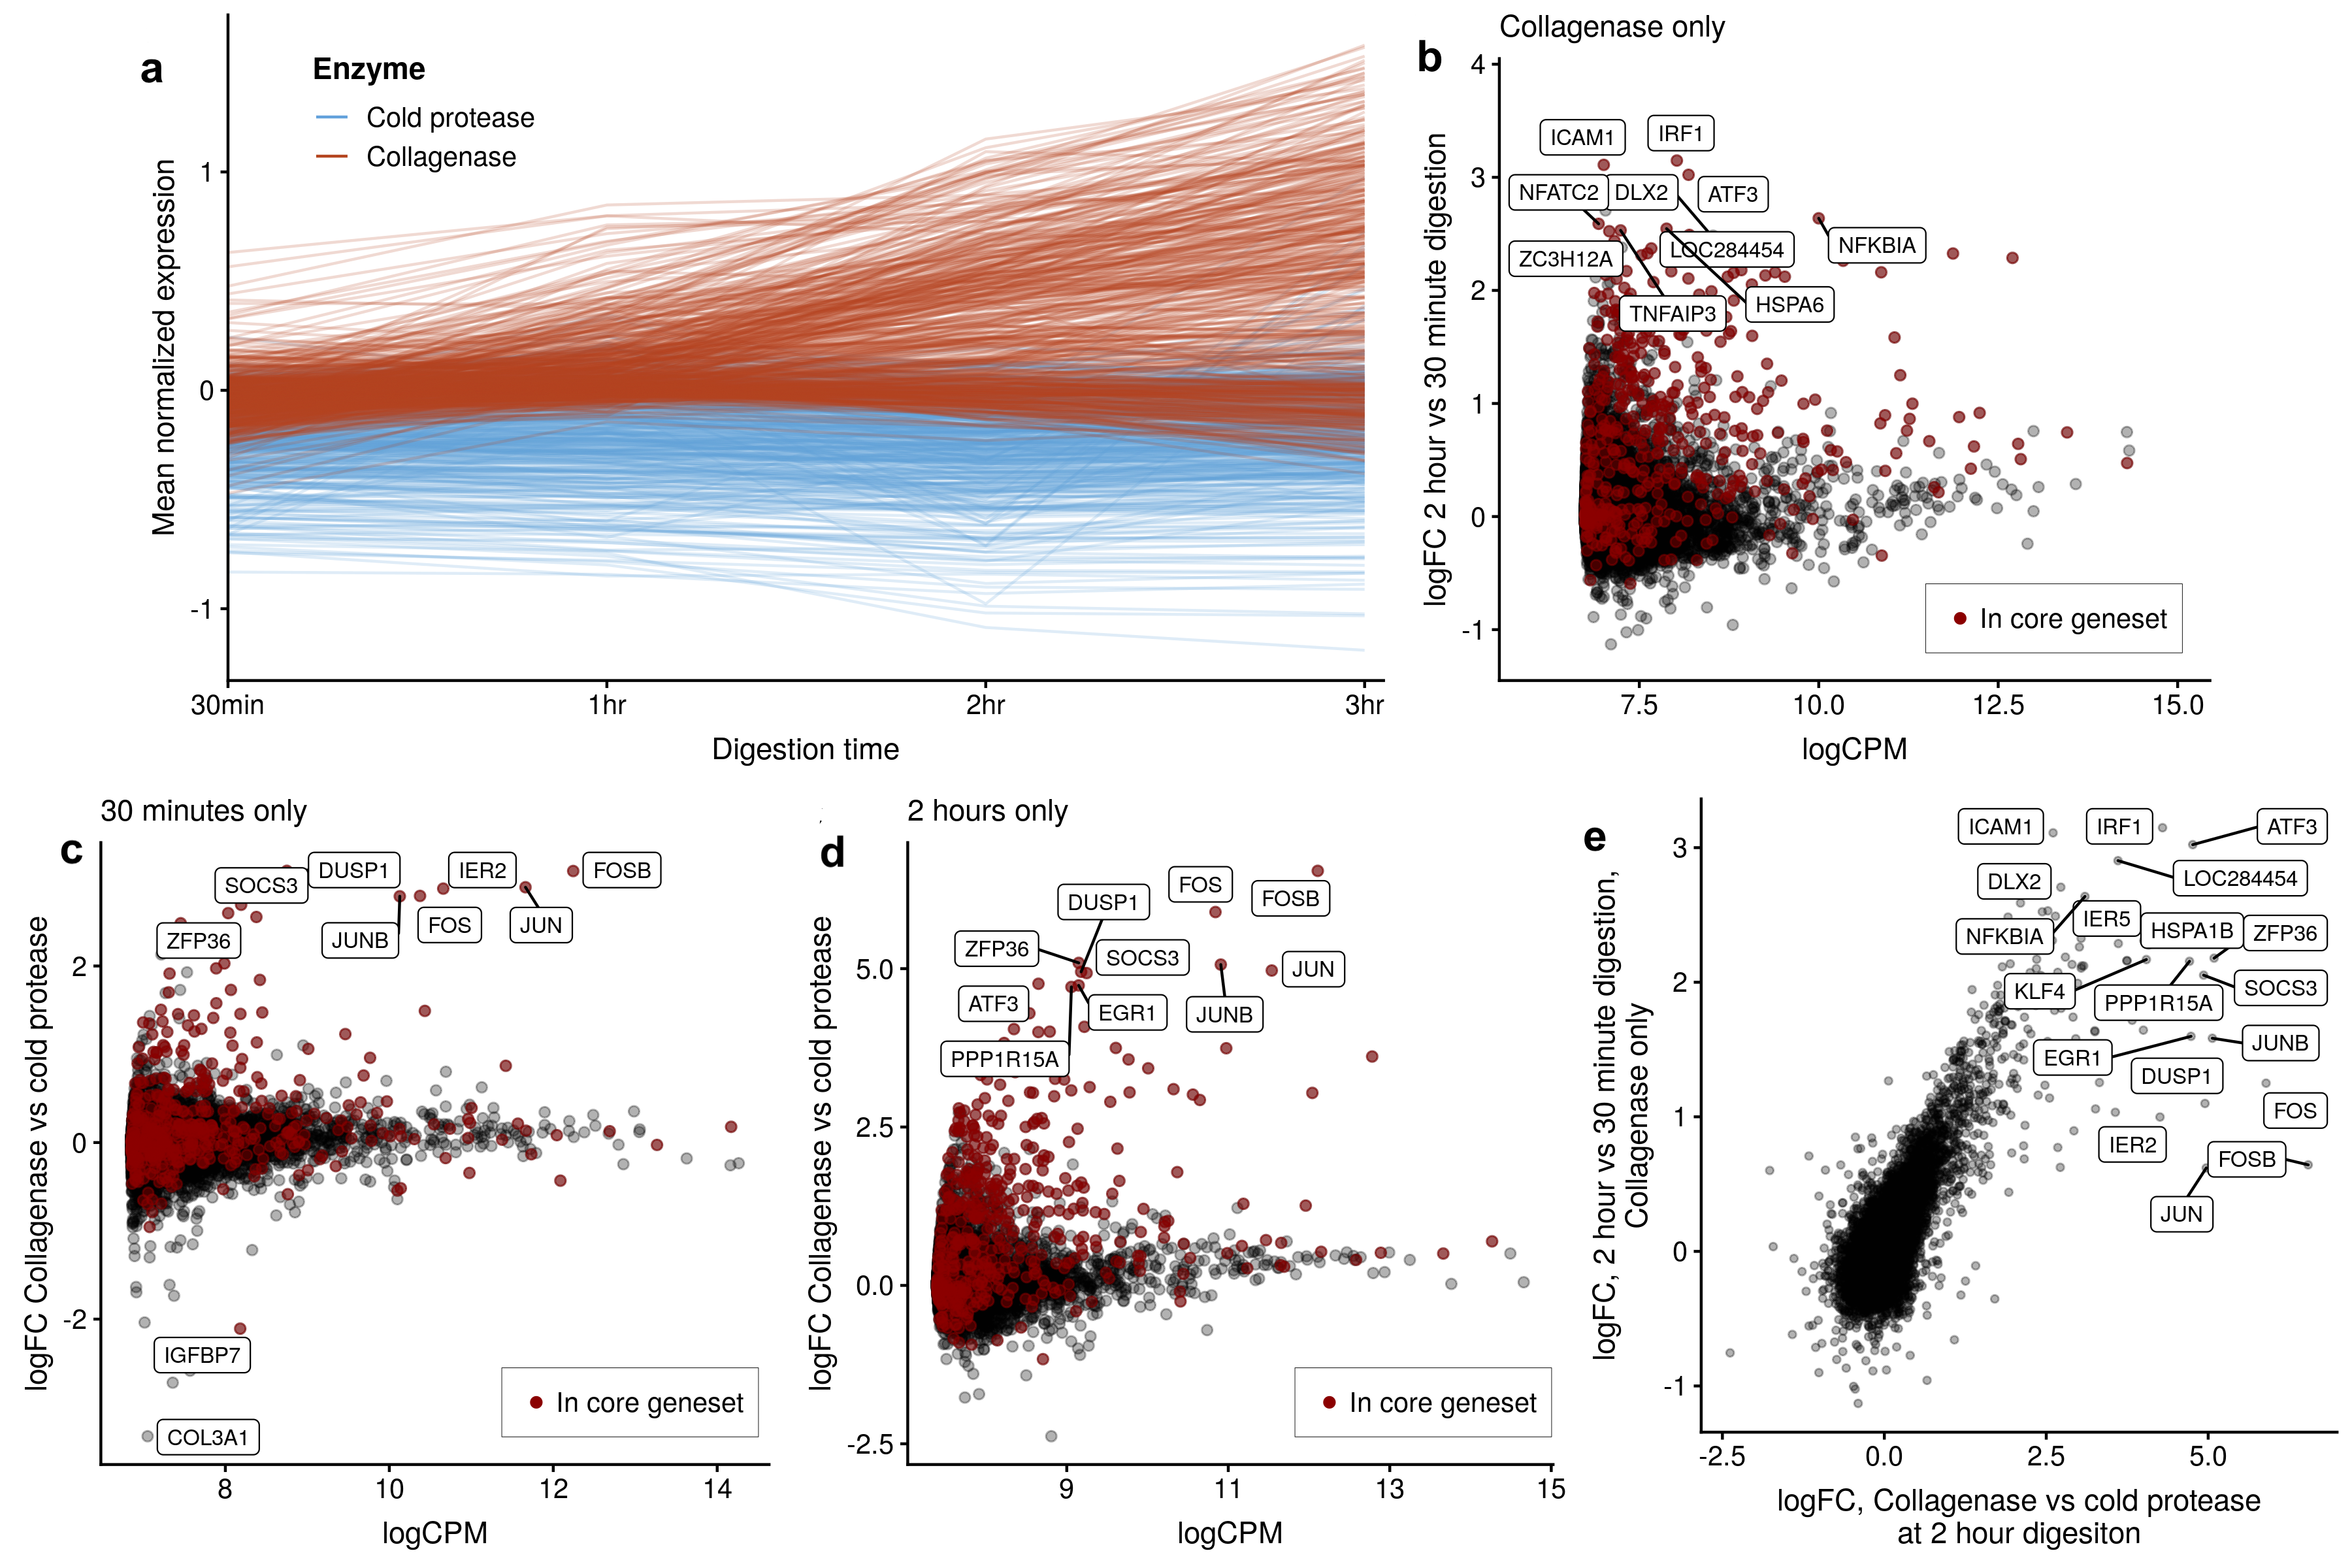
\includegraphics[width=\textwidth]{Figures/chap3/digestiontime.png}
	\caption[Differential expression of cluster 1 of live, dead, and dying cells.]
	{\small
	 \textbf{Disentangling the effects of digestion time and digestion method on transcriptomic response.}
    \textbf{(a)} Mean normalized expression of genes in the core gene set as a function of digestion time coloured by digestion temperature. Digestion by collagenase causes upregulation of the geneset at all timepoints, with a subset showing further upregulation as digestion time increases.
    \textbf{(b)} Log fold changes of a 2 hour vs. 30 minute digestion for collagenase only as a function of log counts-per-million. 
    \textbf{(c)} Log fold changes of a collagenase vs cold protease digestion at 30 minutes digestion time as a function of log counts-per-million. 
    \textbf{(d)} Log fold changes of a collagenase vs cold protease digestion at 2 hours digestion time as a function of log counts-per-million. 
    \textbf{(e)} The log fold changes of a 2 hour vs. 30 minute digestion (collageanse only) compared to a collagenase vs. cold protease digestion at 2 hours demonstrates a large overlap between genes affected ($\rho=$ 0.8).
    }
    \label{fig:digestiontime}
\end{figure}
%----------------------------------------------------------------------


Examining genes identified in the core gene set above, we found striking upregulation of the core gene set between collagenase and cold protease digestion at all digestion times \textbf{(Figure 3.8 a)}. This demonstrates that the choice of digestion enzyme (collagenase vs. cold protease) has an impact on the cells' transcriptional response, independent of the length of digestion. However, a subset of the core gene set was further upregulated with increasing digestion time under collagenase digestion \textbf{\autoref{fig:digestiontime} a)} . To quantify this, we performed several transcriptome-wide pairwise differential expression analyses to discern the effect of digestion conditions on transcriptomic response. Firstly, we compared a 30-min vs. 2 hours digestion using only collagenase \textbf{\autoref{fig:digestiontime} b)} Of the 18,734 genes retained for differential expression analysis, 8,064 (43\%) were significantly differentially expressed ($<5\%$ FDR), with 4917 genes upregulated at 2h and 3,147 downregulated. Of the 512 genes in the core dissociation-associated gene set, 420 (82\%) were significantly differentially expressed (376 upregulated, 44 downregulated).
In contrast, repeating this analysis with cells digested using cold protease only revealed far fewer genes (2,500 of 16,340, 15.3\%) differentially expressed between the two digestion time points, with 35.9\% of the core gene set (70 upregulated, 114 downregulated) showing differential expression over time.
Secondly, we compared collagenase vs. cold protease digestion at 30 min only \textbf{\autoref{fig:digestiontime} c)}. Of the 18,242 genes retained for differential expression analysis, 5039 (27.6\%) were significantly differentially expressed ($<5\%$ FDR), with 2,173 genes upregulated at 2 hours and 2,866 downregulated. Of the 512 genes in the core collagenase-associated gene set, 306 (59.8\%) were significantly differentially expressed (223 upregulated, 83 downregulated). Similarly, comparing collagenase vs. cold protease digestion at  2 hours only \textbf{\autoref{fig:digestiontime} d)} found 7,887 of 17,345 genes (45.5\%) differentially expressed (4,207 upregulated, 3680 downregulated), with 429 of 512 (83.8\%) genes from the core gene set being differentially expressed (362 upregulated, 67 downregulated). These results robustly demonstrate that both digestion time and digestion method contribute to transcriptomic stress response in single cancer cells.
Interestingly, a highly similar set of genes are affected by both digestion time and digestion method, with a large correlation (Spearman's $\rho=$ 0.8) between the log fold changes of contrasting 2-h to 30-min digestion (collagenase only) as compared to a collagenase vs. cold protease digestion at 30 min only \textbf{\autoref{fig:digestiontime} e)}. These results suggest that the cellular response to digestion in single-cell transcriptomic experiments converge on a common set of pathways.


\section{Discussion}
In this chapter, we began with the intention of developing patient derived xenograft (PDX) in immunodeficient NOD Rag-1 null interleukin-2 receptor gamma null (NRG) and identifying the dose response properties of PDX to determine relative ability of the drugs to produce maximum functional response.

To establish PDX models, patient-derived tumors need to be injected into highly immunodeficient mice, because the mouse immune system could eradicate transplanted cancer cells and prohibit tumor engraftment. In order to reach to final formation of longitudinal chemotherapy perturbed model systems, it was important to successfully create PDX in immunodeficient NOD Rag-1 null interleukin-2 receptor gamma null (NRG) instead of highly immunodeficient NOD/SCID/IL2r$\gamma$ $-$/$-$ (NSG). It is by now well known that \ac{NRG} mice can harbor established PDX, and can tolerate aggressive induction chemotherapy at higher doses than NSG mice without overt toxicity \cite{barve2018comparative}. 


Having established tumors in immunodeficient mice, we sought to select breast cancer \ac{PDX} and the chemotherapies that could be used in cancer evolution studies. TNBC-SA609, TNBC-SA1035 and TNBC-SA535 tend to show high sensitivity for platinum so these were selected for making a timeseries model for the next chapter 4. CX-5461, G4 stabilizer drug showed synthetic lethality with DNA repair pathway deficiency in \textit{in vitro} cultures as \cite{xu2017cx}, so along with treating for timeseries with cisplatin, we selected TNBC-SA535 (BRCA1-HRD) for CX-5461 in parallel for timeseries drug perturbation for the next chapter.

Recent advancements in sequencing technologies have allowed for DNA and RNA sequencing at single-cell resolution, which can be used to interrogate genomes and transcriptomes of tumor tissues that may not be resolved by bulk sequencing, such as intratumoral heterogeneity, clonal dynamics, and the mapping of known and de novo cell types. However, various steps can impact the quality and quantity of these single cells for sequencing analysis.
Here we sought to optimize conditions and factors that could participate single cell sequencing outcome. Standard sample preparation methods for solid tissues require enzymatic and mechanical dissociation and, depending on the tissue origin, density, disease state, elastin, or collagen content, may require long enzymatic digestion and/or vigorous mechanical disruption.
For single cell whole genome sequencing the additional step of dead cell removal from the final single cell suspension tend to show  cleaner cells, less debris and high percent viability providing high chances of live cells taken up by the robotic spotters as explained in \cite{laks2019clonal}. 

Current sequencing techniques require single-cell suspensions for passage through microfluidic or microwell platforms, and the generation of single-cell suspensions from solid tissues requires the enzymatic and mechanical disruption of extracellular matrix and cell-cell contacts. To date, the effect of these dissociation methods on the transcriptome of single cells has been largely ignored, despite the potential effects on the interpretation of scRNA-seq data. Moreover, during both dissociation of tissues and passage through fluidic devices, cells can undergo stress, shearing, anoikis, and apoptosis \cite{aljanahi2018introduction}. For this reason, efforts must be made on both sample handling and bioinformatics to ensure minimal noise and optimal filtration of data. Here, we endeavored to describe the artifactual gene expression associated with tissue dissociation and dead or dying cell populations. Using a large, diverse dataset, we highlight the variability in key QC metrics, including the percentage of mitochondrial genes, number of UMIs, and number of genes detected. 

We identified a sub-population of dead cells that would not be removed through standard data filtering practices and quantify the extent to which their transcriptomes differ from live sorted cells
We described sub-populations of dead cells that express either high or low mitochondrial genes, contrary to the notion that dead cells can be characterized by their mitochondrial gene content alone. Importantly, cells that are FACS sorted as either live, dying, or dead based on PI/annexin V staining are present in all three clusters, highlighting that the transcriptomic state of the cell is not necessarily the same as the surface marker state (though the two are correlated). As noted, this is reminiscent of ``pseudotime'' orderings, with PC1 from \textbf{\autoref{fig:livedead} a}  approximating a trajectory through the data that tracks transcriptomically healthy cells to transcriptomically dead cells with increasing PC1 values. Though expressing transcriptomes similar to live, healthy cells, dead cells with low mitochondrial content expressed significantly high levels of MHC class I genes such as HLA-A, HLA-B, and B2M.

 We identified a further sub-population that represents transcriptomically dying cells, expressing increased major histocompatibility complex (MHC)-class I genes. Furthermore, core gene set of immediate, heat shock, and stress response genes associated with collagenase dissociation, highly conserved across cell and tissue types, and which are minimized by dissociation at cold temperature. We suggested that each tissue and dissociation method should be assessed for dissociation-induced signatures before undertaking large-scale scRNA-seq experiments.








{\chapter{Single  cell  whole genome fitness  landscapes  induced  by pharmacologic perturbations in cancer}
}
\label{ch:Chapter4}

\section{Motivation}
As discussed in introduction chapter 1, tumor fitness landscape underpin selection in cancer evolution and response to chemotherapy. However,quantifying fitness in heterogeneous tumor populations remains an open problem that hampers effective treatment leading to tumor recurrence. Previous work has established models of fitness through interpreting allelic measurements of single snapshots \cite{williams2016identification, williams2018quantification,gerstung2020evolutionary,shah2012clonal,nik2012life} from bulk sequencing over large patient cohorts \cite{martincorena2017universal}, timeseries study of cell free DNA \cite{khan2018longitudinal}, multiregion sequencing \cite{Gerlinger2014-qd,Jamal-Hanjani2017-yc,Lopez2020-ku,mcpherson2016divergent,williams2018quantification} and estimating fitness landscapes of clonal haematopoiesis \cite{Watson2020-yu}. Moreover, the cancer field has generally lacked serial measurements from patient derived tissues to directly observe cancer evolution over realistic timescales. This has impeded a thorough understanding of causal factors driving selection, achieved in other biological systems through studying granular timeseries with population genetics modeling \cite{good2017dynamics}. Infact, patient derived xenograft (PDX) systems are an effective model to study timeseries of a human tumour cell population \cite{williams2018using,willey2015patient}.
The majority of the work on cancer has focused on bulk tumour sequencing, where cellular population structure decomposition approaches are limited. Single cell genome measurements to scalably define clonal populations in cancer over thousands of cells have only recently emerged \cite{Laks2019-dm,zahn2017scalable}, enabling identification of rare populations, precise tracking of clones and robust clone-specific measurements suitable for population genetics modeling. We are also motivated by newly developed quantifying tools of sitka, a phylogenetic inference method accompanying toolkits to assign cells to clones, \cite{dorri2020efficient} and  \texttt{fitClone}, a probabilistic framework that designates quantitative selection coefficients to individual cancer clones and forecasts competitive clonal dynamics over time \cite{salehi2020single}. Motivated by these observations, we sought to investigate the hypothesis that clones that grow reproducibly have higher fittness in the growing cancer.

\section{Synopsis}
Based on the knowledge we gained from chapter 3 for transplant efficiency and initial tumor responses to chemotherapies, we selected four \textit{Tp53} mutant \ac{PDX} for this chapter \textbf{\autoref{tab:Tp53mutationofPDX}}. Three TNBC and one HER2+ \ac{PDX} tumors, and two drugs (cisplatin and CX-5461) were selected to investigate clonal dynamics and identify patterns of clonal resistance with single cell whole genome sequencing in treated and untreated timeseries. First we, generated two un-treated transplanted timeseries PDX (SA532-HER2+ and SA609-TNBC) from passage one (X1) to passage ten (X10) to test the newly developed methods for identifying sub-populations with their genotypes. 
We showed that serial measurements of single cell copy number assigned clones can be used to estimate fitness in conjunction with \texttt{fitClone} \cite{salehi2020single}, under serial transplantation of breast patient derived xenografts, where no drug selection or other conditions were applied. We found that serial measurements can be used to measure relative clonal fitness which enables prediction of future trajectories.

Next we sought to  confirm the reproducibility and independence of dynamics to population size effects, we re-ran the serial transplantation experiments after mixing early and late populations and re-measuring the dynamical behaviour. We observed that sufficiently well sampled clones with confident fitness estimations show repeated trajectories, confirming the estimation of fitness and linking the dynamical behaviour to the copy number genotypes of the clones.

Finally, we determined whether the fitness of clones under chemotherapy can be measured and asked whether clones exhibiting drug resistance are also fitter in the absence of selective pressure from chemotherapy. 

On all the single cell whole genome sequencing data, we applied three types of scientific computational methodologies. First, \textbf{sitka}, for computing phylogenetic trees and identifying genotypic clones, then using \textbf{Lumberjack} (a tree-cutting algorithm) and their relative abundances as a function of time. Last, \texttt{fitClone}, to measure the selection coefficient for each clone \textit{s} which we hypothesise to indicate growth potential. The larger the value of \textit{s}, the more fit the clone is relative to the chosen reference clone. 


 % Table generated by Excel2LaTeX from sheet 'Tp53_PDX_mutation_small'
 \begin{table}[htbp]
   \centering
   \caption{\textit{Tp53} mutation status of all PDX}
     \begin{tabular}{|l|l|l|l|}
     \hline
     Sample ID & Protein Change & p53 Mutation Type & HGVSg \\
     \hline
     SA1035-TNBC  & C242F & Missense\_Mutation & 17:g.7577556C>A \\
     SA609-TNBC & R213* & Nonsense\_Mutation & 17:g.7578212G>A \\
     SA532-HER2+ & A159P & Missense\_Mutation & 17:g.7578455C>G \\
     SA535-TNBC & V147Gfs*2 & Frame\_Shift\_Ins & 17:g.7578490\_7578489insC \\
     \hline
     \end{tabular}%
   \label{tab:Tp53mutationofPDX}%
 \end{table}%











%...........................................................





\section{Results}

 
\subsection{Establishment of untreated timeseries patient derived xenografts}
Taking multiple measurements is critical for understanding  given behavior of cancer clones that are forced to evolve over time, and doing so at equal intervals give an open opportunity to clearly investigate the dynamics of that behavior manifesting at distinct time scales. 
To understand and quantify fitness attributes of cancer cells as  predictive measures of their growth potential in polyclonal systems, we set out to establish time series patient derived xenografts (PDX) with and without pharmacological perturbations.
Serial transplantations were performed by injecting patient derived tumor cells and clumps into primary engrafted mice to secondary and subsequent recipients in a time series manner \textbf{(\autoref{fig:Untreatedgrowthcurves}, n=3-4 at each time point)}. We passaged two PDX, SA532 (HER2+) and SA609 (TNBC), till tenth generation (X1-X10). X1 represents passage one (first generation) of the PDX and X10 as last passage (tenth generation)   \textbf{(\autoref{fig:Untreatedgrowthcurves} a)}. 
Tumor growth measurements record from both PDX serries exhibited increased growth rate in later passages as compared to early passages \textbf{(\autoref{fig:Untreatedgrowthcurves} b)}.
 
 
 \begin{figure}
\centering
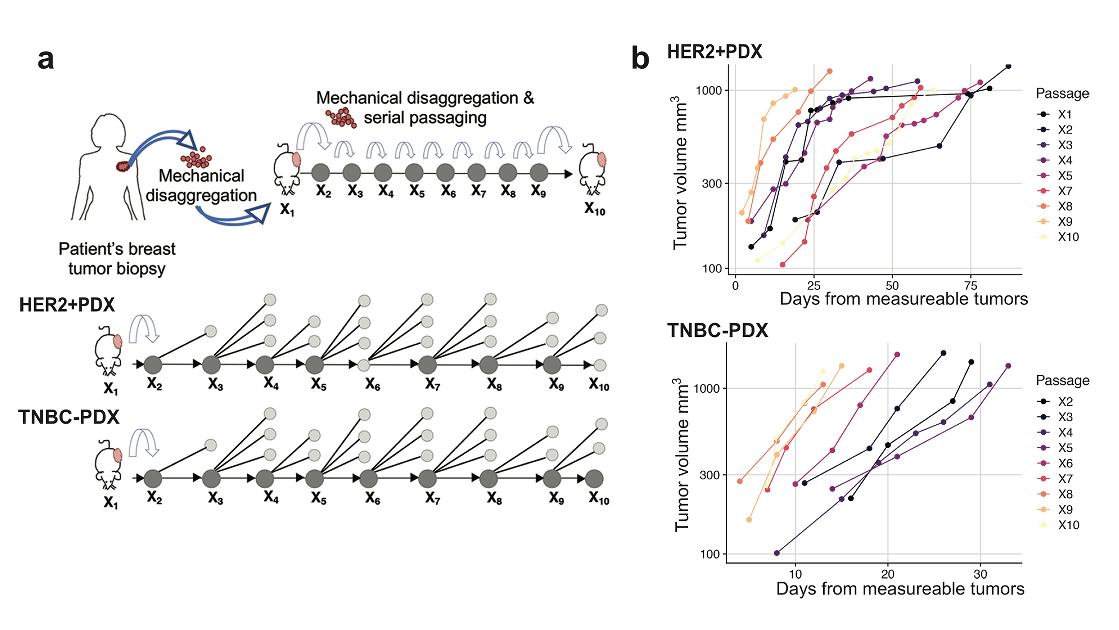
\includegraphics[width=\textwidth]{Figures/Untreatedgrowthcurves.pdf}
	
\caption[Untreated PDX timeseries and growth trajectories]
	{\small
	\textbf{Untreated PDX timeseries and growth trajectories.}
	    \textbf{(a)}, Top: Schematic for PDX timeseries; Bottom: Serial sampling of HER2+ and TNBC PDX tumours;
Dark grey circles represent each sampled mouse for scWGS. The light grey circles representing the replicates of tumour-bearing mice at the same timepoint. Small light grey at X6 and X10 represents absent data points.
	    \textbf{(b)}, Individual tumour growth from each passage of TNBC and HER2+ PDXs. Y-axis is showing the tumor volume in cubic millimeter while the x-axis is representing the time in days, tumors could be measured.}
	\label{fig:Untreatedgrowthcurves}
\end{figure}



\begin{figure}
\centering
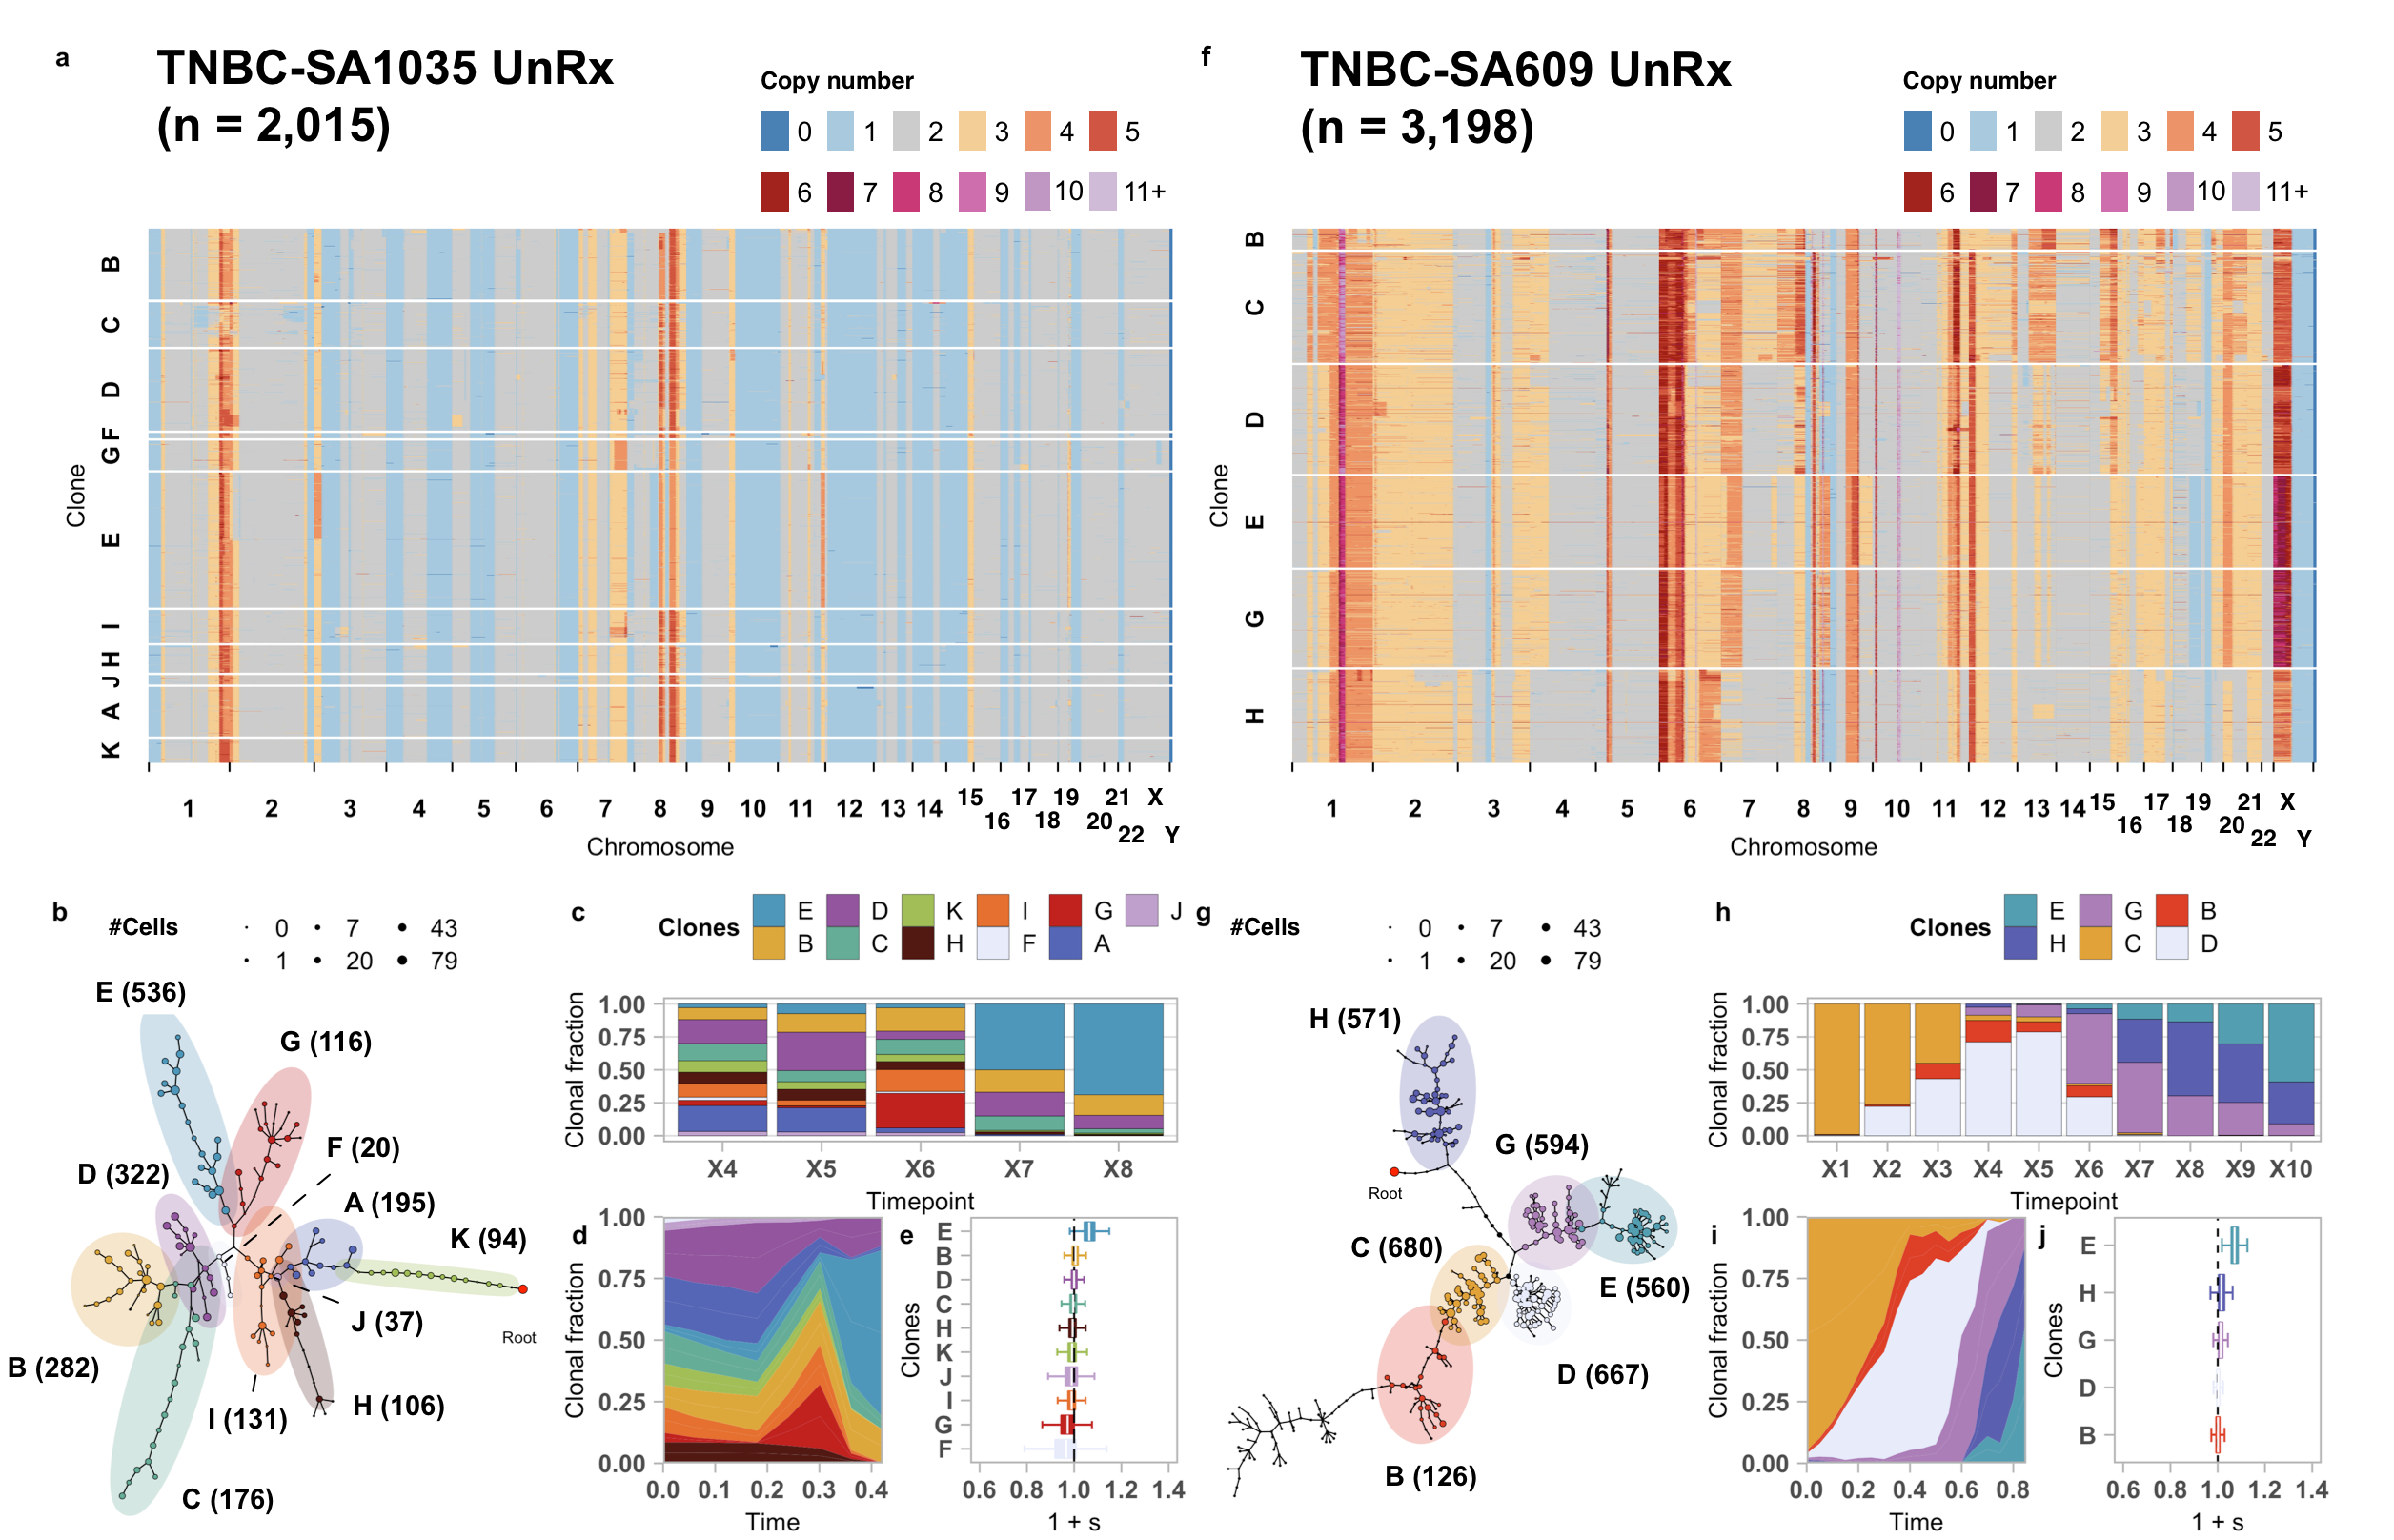
\includegraphics[width=\textwidth]{Figures/UnRxseries.pdf}
	
\caption[Untreated PDX timeseries clonal dynamics at single cell level]
	{\small
	\textbf{Comparison of fitness landscapes of two untreated breast cancer PDX timeseries models.}
	    \textbf{(a, b)} Clonal dynamics of HER2+ and TNBC models.
	    \textbf{(c)} Probability of positive selection in both PDX
	    \textbf{(d)} Heatmap representation of copy number profiles of 2,193 cells, grouped in 4 phylogenetic clades. 
	    \textbf{(e)} Phylogeny (simplified type II sitka tree) of cells over the timeseries HER2+ Untreated PDX, where nodes are groups of cells (scaled in size by number) with shared copy number genotype and edges represent distinct genomic copy number change points (sitka markers)
 
\textbf{(f)} Top: growth trajectories, Bottom: Inferred \texttt{fitClone} trajectories
\textbf{(g)} selection coefficients for the HER2+ model. 
 \textbf{(h-k)} Analogous plots for the TNBC model (n=3,216 cells).
 
	}
	\label{fig:UnRxseries}
\end{figure}


 Patient's tumor architecture and integrity was confirmed on H \& E and immuno-histochemistry staining of paraffin embedded tumor sections at each time point with a set of standard markers. \textbf{(See Methods, {\autoref{fig:HistologyHER2+TNBC}} a, b)} showing representative images of initial and late passages of tumor sections.

\subsection{Clone-specific fitness estimates forecast clonal competition trajectories} 
 
 We next generated single cell whole genomes from 10 serial PDX transplants over 721 days from a HER2+ breast cancer with a \textit{TP53} p.A159P missense mutation, and contrasted this with 10 serial samples over 1002 days from a basal-like \ac{TNBC} PDX with a \textit{TP53} p.R213* non-sense mutation. Two time points, X6 and X10 from HER2 positive PDX failed to produce successful library so those were removed during analysis. Clonal expansions observed during serial passaging of \textit{TP53} mutant PDX tumours to determine the predictive capacity of fitness coefficients \textbf{\autoref{fig:Mixturenew}}.
A median of 907 single cell genomes were sequenced per passage for a total of 11,705 and 10,553 single cell genomes from the HER2+ and TNBC series, respectively. 


\subsubsection{Phylogenetics and fitness analysis on single cell whole genome data}
For each of the two timeseries PDX (HER2+ and TNBC), we inferred single cell copy number profiles , constructed a phylogenetic tree using \textbf{sitka} model taking copy number states as input to establish clonal lineages and measured clonal abundances as a function of time \textbf{(\autoref{fig:UnRxseries} a, b, c)}. For each timeseries (branch), we pulled all single cells to infer a phylogenetic tree \textbf{(See introduction and methods for details)}. The tree was cut using Lumberjack to yield clones and their abundances over time. Then \texttt{fitClone} inferred selection coefficient of a clone by reporting the posterior mean 1 + s followed by its standard deviation.

\subsubsection{Untreated timeseries SA532 HER2+ PDX undergo neutral clonal dynamics}

 The SA532 HER2+ series exhibited 4 distinct clones ranging in size from 134 to 1,421 cells (median 319, \textbf{(median 319, \autoref{fig:UnRxseries} e)}, and the TNBC series exhibited 8 distinct clones with 18 to 680 cells (median 556, \textbf{(\autoref{fig:UnRxseries} i)}. Clonal trajectories in the HER2+ model, were consistent with selective coefficients with small relative differences in fitness \textbf{(\autoref{fig:UnRxseries} f, g)}.
 We observed a small decrease of 0.04 copy number breakpoints per generation (linear regression, p=0.002,=0.05). 

\subsubsection{Untreated timeseries SA609 TNBC PDX undergo deterministic clonal dynamics}
In contrast to HER2+ timeseries, the TNBC model trajectories resulted in a high positive selective coefficient for a minority of clones \textbf{(\autoref{fig:UnRxseries} j, k)} mean = 1.03 $\pm $0.11. Consistent with increased dynamics in the TNBC series, we found an initial increase of 0.1 breakpoints per cell per generation in the first 4 passages \textbf{(\autoref{fig:mutationanalysisbreakpoints} a)}. After this initial increase the average number of breakpoints per cell remained constant.
 Clone E in TNBC swept the population over the last 3 timepoints \textbf{(\autoref{fig:UnRxseries} j, k)} (n=541 over the timeseries). Clone E had the highest selective coefficient (1+s= 1.08 $\pm $ 0.043), having grown from undetectable proportions in earlier timepoints to 58\% of cells by the end of the timeseries. Clone E also had the highest number of breakpoints with 12.8 additional copy number breakpoints per cell, relative to the reference clone C with the lowest (linear regression with coverage breadth, ploidy and cell cycle state as covariates (p $<$0.0001) \textbf{(\autoref{fig:mutationanalysisbreakpoints} c)}.


\subsection{SA609-TNBC mixture timeseries yielded selection of biologically similar population}
We next asked whether the high predicted fitness of Clone E was a true indicator of positive selection through a physical clonal mixing and re-transplant experiment. Enforced clonal competition of higher fitness clones with lower fitness counterparts should result in re-emergence or fixation of high fitness clones, even when re-starting from a low population prevalence. To test this, we performed mixture experiments by extracting cells from an early (X3) and a late (X8) passage of SA609 TNBC timeseries PDX and then physically mix them. We established two such lines with different proportions \textbf{(also see methods)}.
In first branch a, we aimed to have a mixture comprising approximately of equal proportions from the two timepoints ($\approx$~50\% each) at the ratio of 1:1. In branch b, we aimed to have far less cells from late passage that contains the high fitness clone. The (71\% of X3 passage and 29.0\% of cells from the X8 passage) a ratio of 1:0.4.


\subsubsection{Clones with higher selection coefficients out compete low fitness clones in mixture branch a}
We forward-simulated trajectories from \texttt{fitClone} using the median of the posterior distribution of the estimated selection coefficients (F = -0.01  $\pm$ 0.13, A = -0.00 $\pm$ 0.16, B= 0.00 $\pm$  0.01, D = 0.00  $\pm$  0.01, G = 0.02  $\pm$  0.02, H = 0.03  $\pm$  0.03, E = 0.08  $\pm$ 0.10) and starting clonal proportions of (A=0.000 (no observed cells), B=0.07, C=0.25, D=0.51, E=0.02, F=0.000 (no observed cells), G=0.08 H=0.07) \textbf{\autoref{fig:Mixturenew} a}. The starting clonal proportions were inferred by adding the cells from the initial passage (M0) to the tree inferred from the cells in the original series (TNBC-SA609) and assigning them to their respective clones. We generated 10,000 trajectories from the model. \textbf{\autoref{fig:Mixturenew} c, f} shows the simulated trajectories in black.
The mean clonal fraction at each step is shown in red. All clones except for clones E, D, and F are predicted to vanish to clonal fractions of below 1\%. We have combined the trajectories for clones E and F since clone F (i) had fewer than 19 total cells in the original series and consequently its selection coefficient had a high variance, (ii) is phylogenetically proximal to clone E \textbf{\autoref{fig:Mixturenew} b} and thus likely represented a biologically similar population and (iii) finally, is not observed above a threshold of 20 cells in any other line in the TNBC-SA609 family.

We experimentally tested these predictions by initiating a new PDX line with the remixed population (from M0), serially passaged over 4 timepoints \textbf{\autoref{fig:Mixturenew} a} (top), and sequenced with DLP+ (7,839 single cell genomes, median 1,354.5 per library). After placing the cells from all timepoints of this mixture experiment on the tree, they got assigned to seven clones from the original timeseries (all but clone A) between 26 to 499 (median 162) cells \textbf{\autoref{fig:Mixturenew} d} . In \textbf{\autoref{fig:Mixturenew} c, f} blue dots show the observed clonal fractions at each timepoint in PDX branch a. Clones with higher selection co-efficients swept through the mixture timeseries by passage 4 \textbf{(\autoref{fig:Mixturenew} e)}. In the last timepoint, the clade composed of clones E and F comprised 94\% of cells, outcompeting low-fitness clones. The estimated selection co-efficients were relatively strongly correlated (Pearson correlation of 0.795, considering only clones that reached overall prevalence of over 1\% in the original series, i.e., all clones except A and F.


\begin{figure}
\centering
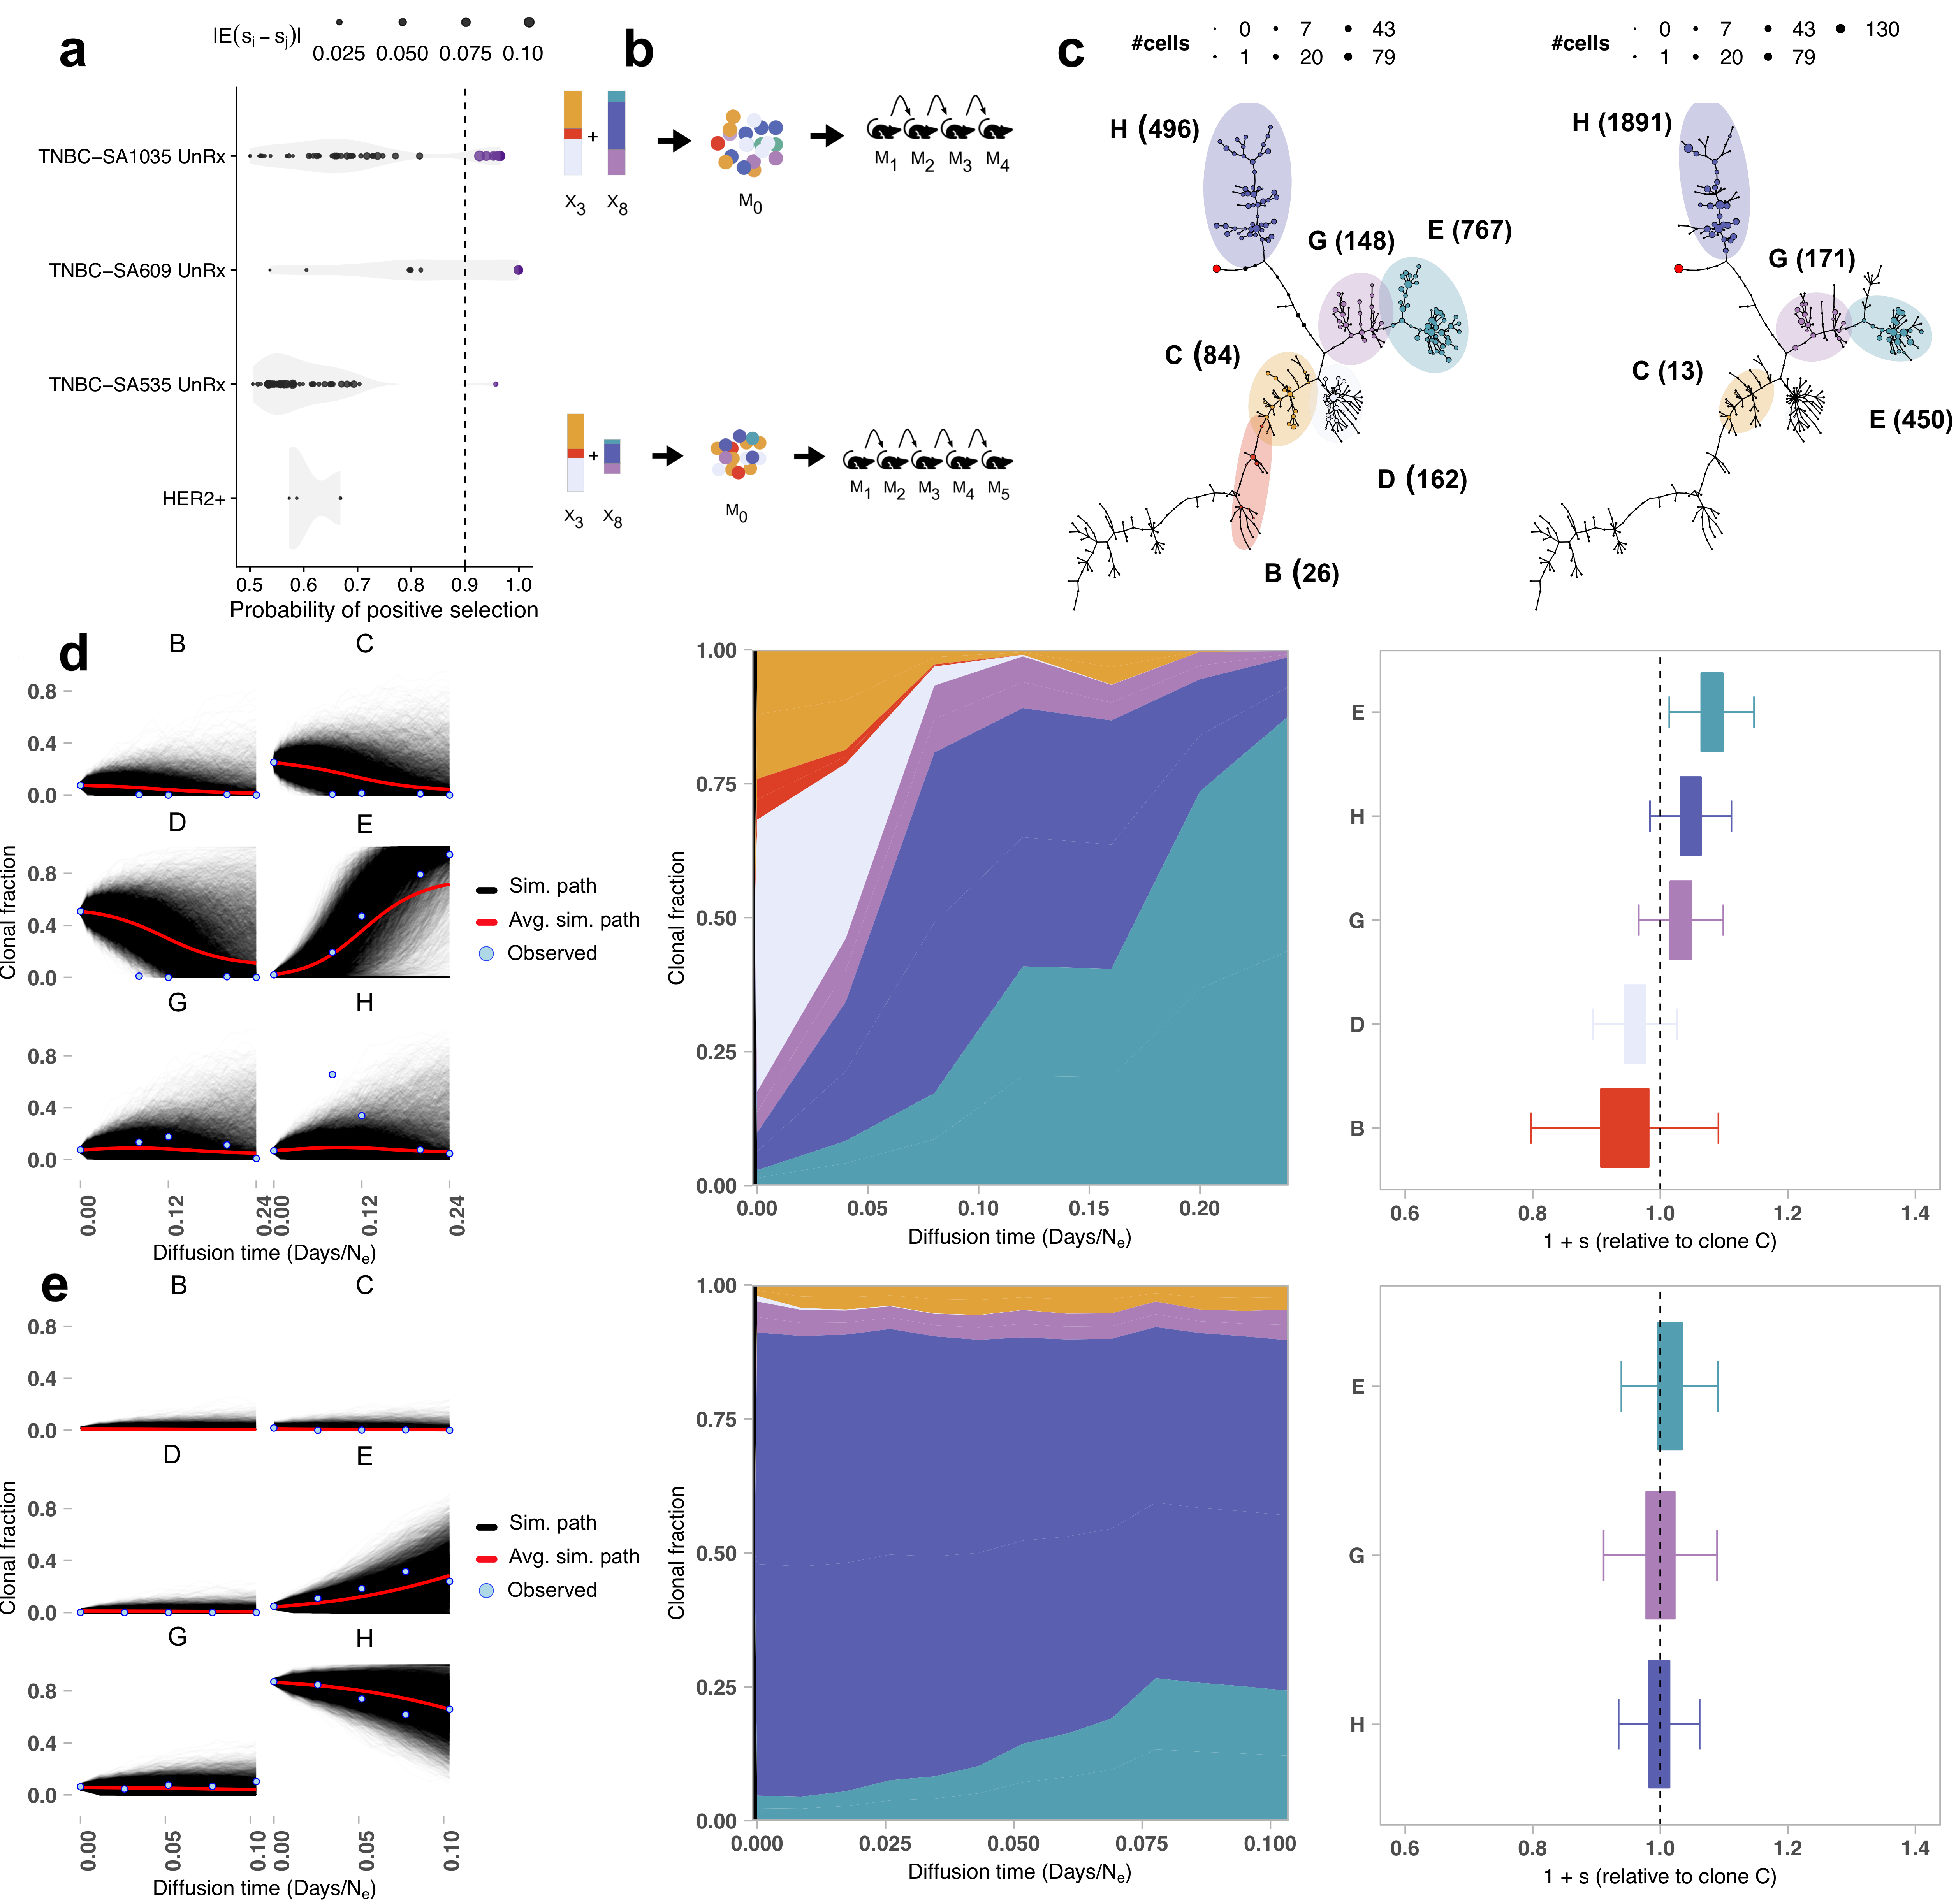
\includegraphics[width=\textwidth]{Figures/Mixturenew.png}
	
\caption[Reproducible dynamics from SA609-TNBC mixture experiments]
	{\small
	\textbf{Reproducible dynamics from SA609-TNBC mixture experiments}
	    \textbf{(a)} Clonal proportions of X3 and X8 to generate the initial mixture M0 and subsequent serial passaging, yielding 4 samples M1-M4 for mixture a and 5 samples
M1-M5 for mixture b.
	    \textbf{(b)} Phylogenies showing cells observed in the mixture a (left) and mixture b (right) timeseries.
	     \textbf{(c)} For mixture a: Forward simulations using inferred selection coefficients and starting population proportions in the initial experimental mixture. Red line representing the time-axis for the observations that is shrunk to best match the mean predicted trajectories
	     \textbf{(d)} Inferred trajectories of mixture a timeseries \textbf{(e)} Selection coefficients of \texttt{fitClone} fit to M1-M4 clonal abundance observations.
 \textbf{(f)} For mixture b: Forward simulations using inferred selection coefficients and starting population proportions in the initial experimental mixture
  \textbf{(g)} Inferred trajectories of mixture b timeseries
	  \textbf{(h)} Selection coefficients of \texttt{fitClone} fit to
M1-M5 clonal abundance observations.    
}
	\label{fig:Mixturenew}
\end{figure}


\subsubsection{Mixture branch b recapitulates the predicted dynamics of branch a and the original untreated branch}
We forward simulated 10,000 trajectories using identical selection coefficient values as the first mixture branch a, but different clonal proportions, estimated from adding cells from timepoint X1 in mixture branch b to the TNBC-SA609 phylogenetic tree and assigning them to the corresponding clones (C = 0.02, D = 0.00, E = 0.05, F = 0.00, G = 0.06, H = 0.87). Unlike mixture branch a, DLP+ data was not available for timepoint M0 in mixture branch b. We generated a timeseries PDX passaged over 5 timepoints that were sequenced using the DLP+ platform to generate 6,730 single cell genomes (median 1,270 per library). We observed 6 clones from the original series, namely all clones except A and B. However, we only captured over the 5 timepoints, 1 cell from clone D, 8 cells from clone F, and 13 cells from clone C. As predicted, clone E, which had the highest predicted selection coefficient in the original series despite having started from a very low clonal fraction (0.05), rises to an abundance of 0.28, while clone H steadily falls from 0.87 to about 0.67 \textbf{(\autoref{fig:Mixturenew} g, h)}.

The analysis of the two mixture series suggests that (i) we can validate the selection coefficients estimated from a timeseries using \texttt{fitClone} and (ii) it is possible make quantitative predictions about the likely trajectories of tumour subpopulations at least at the clade level. Also, in the prediction trajectories plot \textbf{(\autoref{fig:Mixturenew} c, f)}, the time-axis for the observations is shrunk to best match the mean predicted trajectories line (red line). The diffusion time horizon that is obtained by dividing the generation time measured in days by the effective population size estimate results in trajectories that are ahead of the biological system. While in branch a the original time horizon is 0.24 and the best matching time is 0.20, in branch b the values are 0.23 and 0.08 respectively.





\begin{figure}
\centering
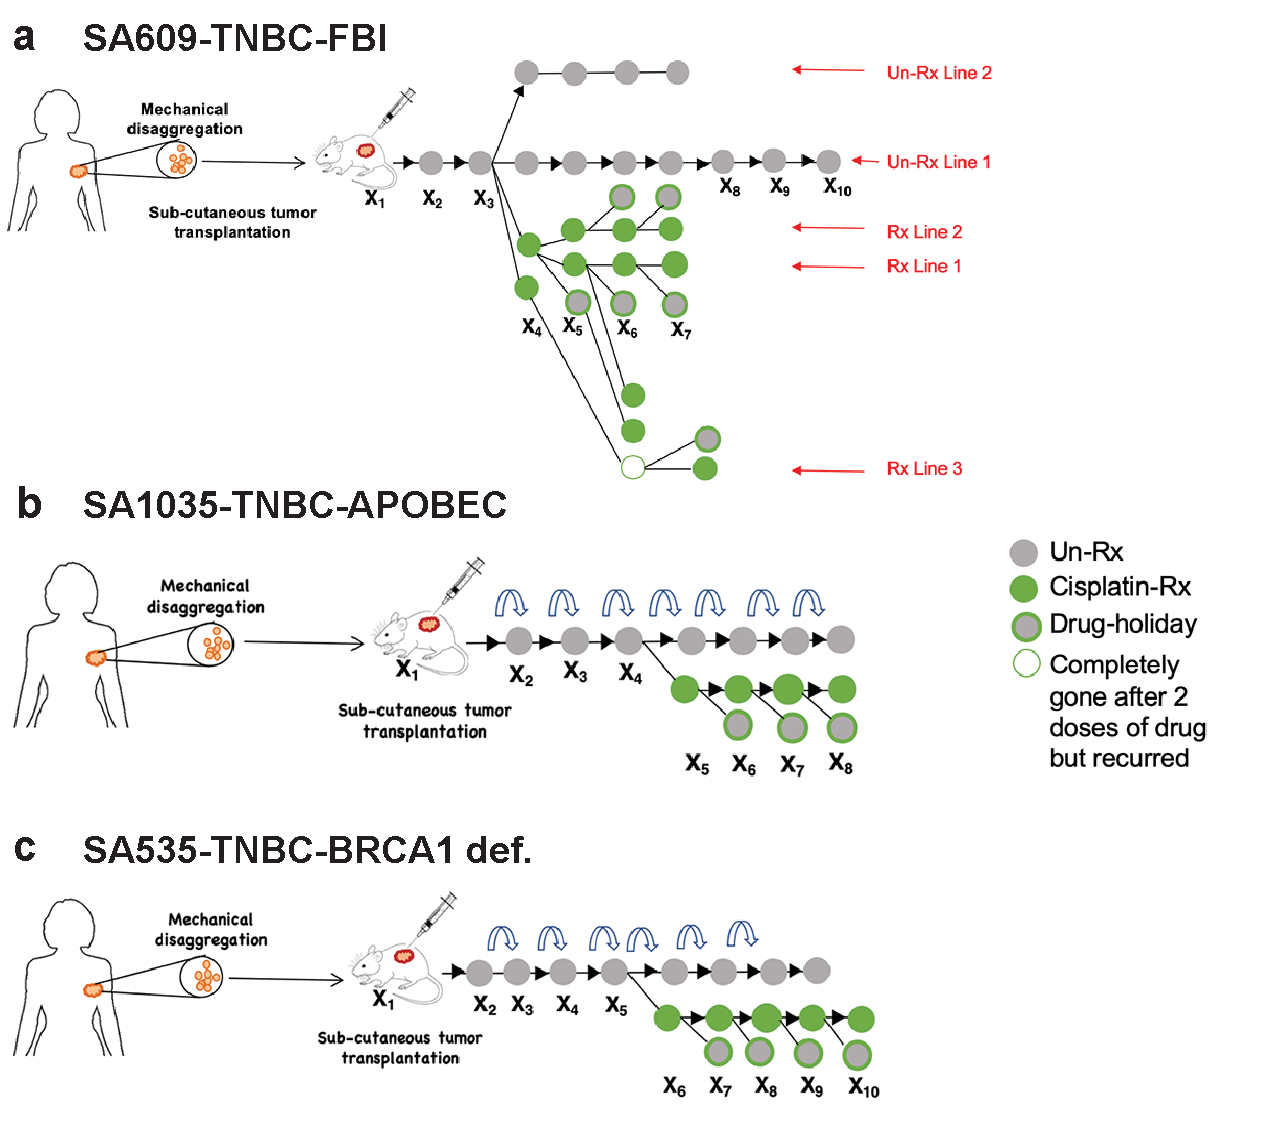
\includegraphics[width=\textwidth]{Figures/treatedtimeseriesgreen.pdf}
	
\caption[Experimental overview of TNBC PDX treated time series]
	{\small
	\textbf{Experimental overview of TNBC PDX treated time series.}
	      All nodes representing each PDX tumour were digested to acquire genomes of single cells (~200-600 cells/tumor). Extra replicate tumors at each time point are not shown in the diagram (n=2-4). Grey circles represent un-treated, green represents Cisplatin treated and grey with green outline presents drug-holiday samples \textbf{(a)} SA609-TNBC time series with replicate treated and un-treated branches. DLP+ collected starting from X1 to X10 (Un-Rx line 1). Top grey branch indicating Un-Rx line 2. The middle three branches are cisplatin treated time series replicate branches \textbf{(b)} SA535-TNBC  showing the tumor nodes taken for DLP+ starting from X5 untreated \textbf{(c)} SA1035-TNBC  showing the tumor nodes taken for DLP+ starting from X 4 untreated.}
	
	\label{fig:treatedtimeseriesgreen}
\end{figure}

%...............................................................
\subsection{Clonal competition and fitness costs of platinum resistance}
So far we have applied our framework to pharmacologically unperturbed tumor environment to track human cancer clones as identified by their Copy number genotypes over time and to reason about their likely abundances and validating them with various experimental conditions. Now we investigate whether establishing baseline fitness measures could help to interpret selection under drug administration. We first present the TNBC-SA609 series in detail and make an observation about early response to cisplatin treatment. We then analyse two
additional TNBC PDX lines to check the reproducibility  and generalizability of our observation.

\subsubsection{Repeated platinum exposure causes less tumor responsiveness} 
 To test pharmacologic perturbation with cisplatin (platinum) impacted the stability of the fitness landscape of the TNBC series, we generated a separate branch of the SA609-TNBC PDX model where we administered cisplatin (2mg/kg, \textit{Q3Dx8} i.p. max) serially over four successive passages to induce drug resistance along with its un treated control branch. For each serially treated tumour, a parallel set of transplanted mice were left untreated, establishing corresponding drug ‘holiday’ samples (\textbf{See methods for detailed experimental design \textbf{1.1.4}, \textbf{\autoref{fig:treatmentdesignMTD} a)}}. Briefly, We coded the treated passages with `T' and untreated with `U' initialised by the X3 untreated (U) passage in SA609 TNBC, X4 untreated (U) in SA1035 TNBC and X5 untreated (U) in SA535 TNBC \textbf{\autoref{fig:treatedtimeseriesgreen} a, b, c}. In SA609 TNBC, the first treatment passage(\textit{X4 UT}) exhibited rapid tumour shrinkage (>50\% of initial size). However \textit{X5 UTT}, \textit{X6 UTTT} and \textit{X7 UTTTT} had progressively less response, indicating drug resistance and positive growth kinetics \textbf{(\autoref{fig:SA609allcyclescisplatin})}. 


\subsubsection{A new clone evolved and swept to fixation with increasing platinum cycles in SA609-TNBC PDX}
Decomposing the growth dynamics over (\textit{X3 U}; \textit{X4 UT}; \textit{X5 UTT}; \textit{X6 UTTT}; \textit{X7 UTTTT}) into clonal trajectories with DLP+ analysis suggested sustained cisplatin treatment inverted the fitness landscape. A new Clone R,  derived from Clone A in the phylogeny, but with a distinct clonal genotype (fewer copies of \textit{MYC} and deletions at \textit{RB1}, \textit{PRDM9} and \textit{NUDT15} loci, \textbf{\autoref{fig:drugholidayfitnesscost} a, b)}, swept to fixation comprising 48\% (\textit{X4 UT}), 98\% (\textit{X5 UTT}), 100\% (\textit{X6 UTTT}) and 100\% (\textit{X7 UTTTT}) of cells across the treated series \textbf{(\autoref{fig:drugholidayfitnesscost} c)}. Notably, the high fitness clones E, H, G, D from the untreated series exhibited low fitness coefficients in the treatment series and were no longer detected \textbf{(\autoref{fig:drugholidayfitnesscost} d}, \textbf{\autoref{fig:landscapefitness})}. Conversely, Clones A, and B, comprising a low fitness phylogenetic superclade, distinct from high fitness clones E and F in the untreated series, were the precursors to the resistant clone R \textbf{(\autoref{fig:SA609Rxnew} d)},    \textbf{(\autoref{fig:landscapefitness})} Thus, cisplatin perturbation resulted in a near complete inversion of the fitness landscape.

%....................................................................


\begin{figure}
\centering
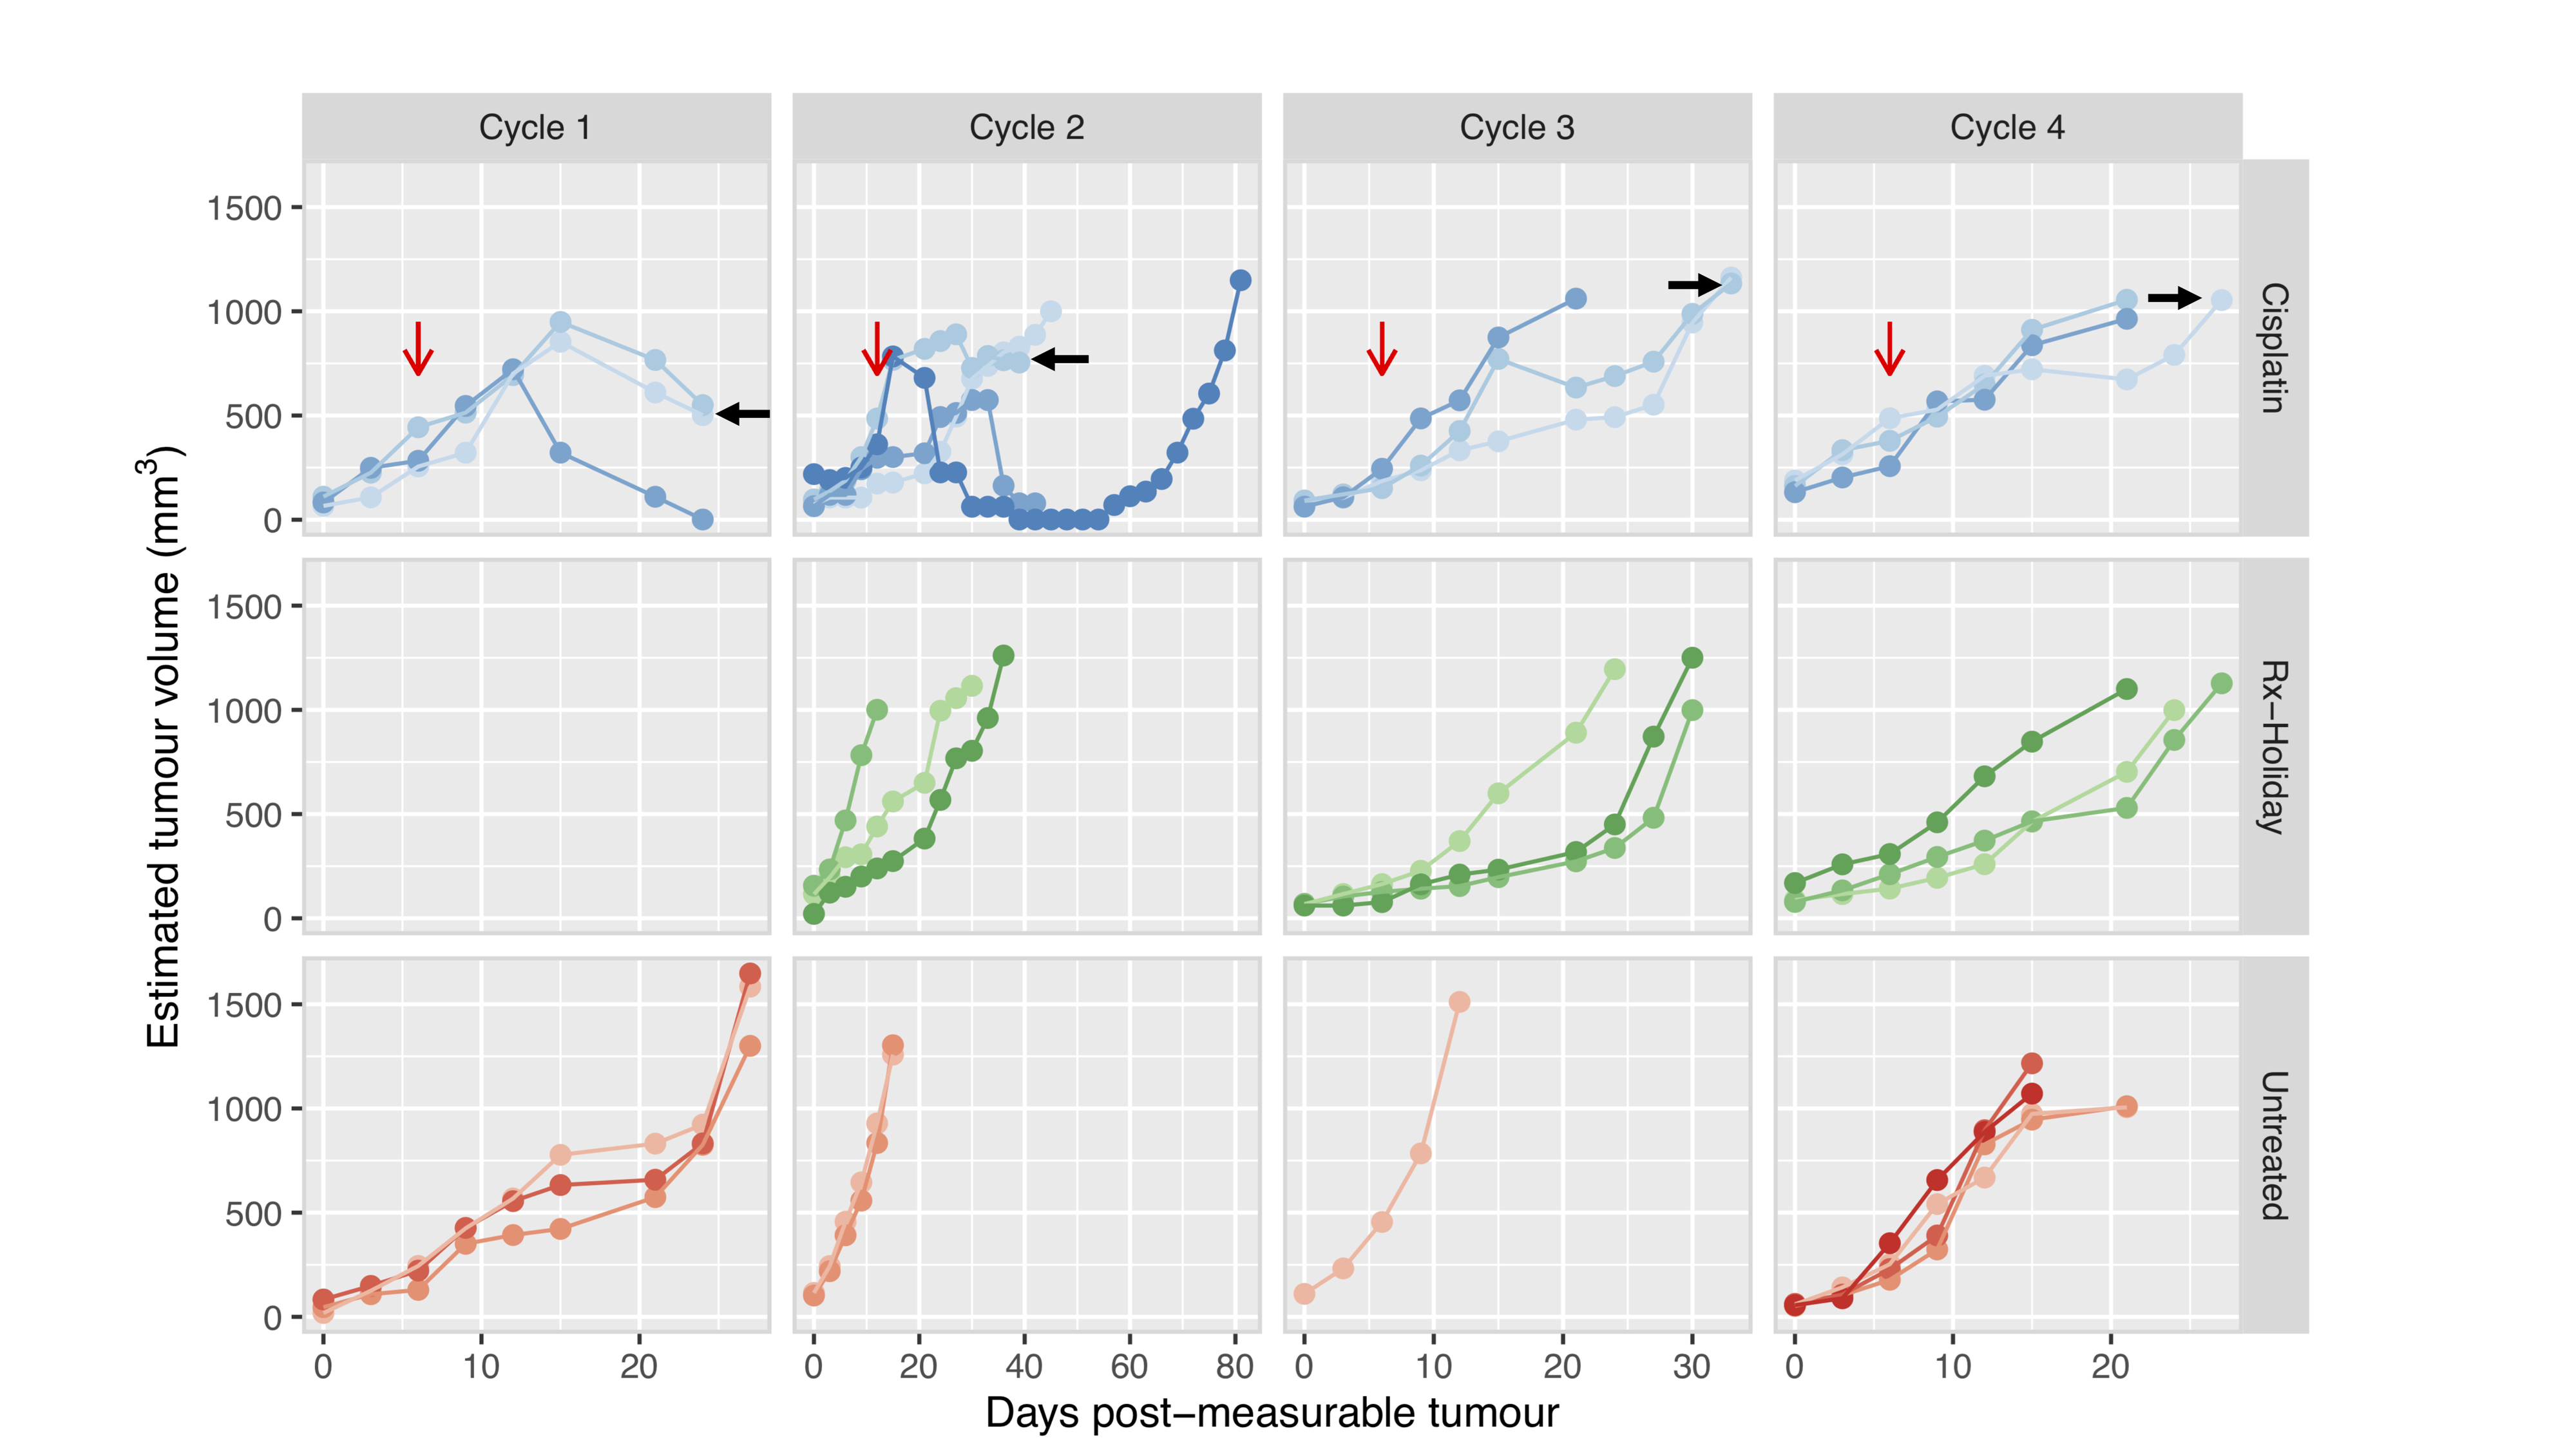
\includegraphics[width=\textwidth]{Figures/SA609allcyclescisplatin.pdf}
	
\caption[Representative growth curves from SA609 TNBC treated with cisplatin]
	{\small
	\textbf{Growth curves from SA609 TNBC treated with cisplatin.}
	   The vertical axis on the left side presents the tumor volume in cubic millimeters and on the right side presents the type of mice groups and their treatment status. Red arrows in the top panel indicates the time treatment started and black arrows indicate the tumor that was taken to re transplant in the next generation of mice.
	}
	\label{fig:SA609allcyclescisplatin}
\end{figure}


%....................................................................


\begin{figure}
\centering
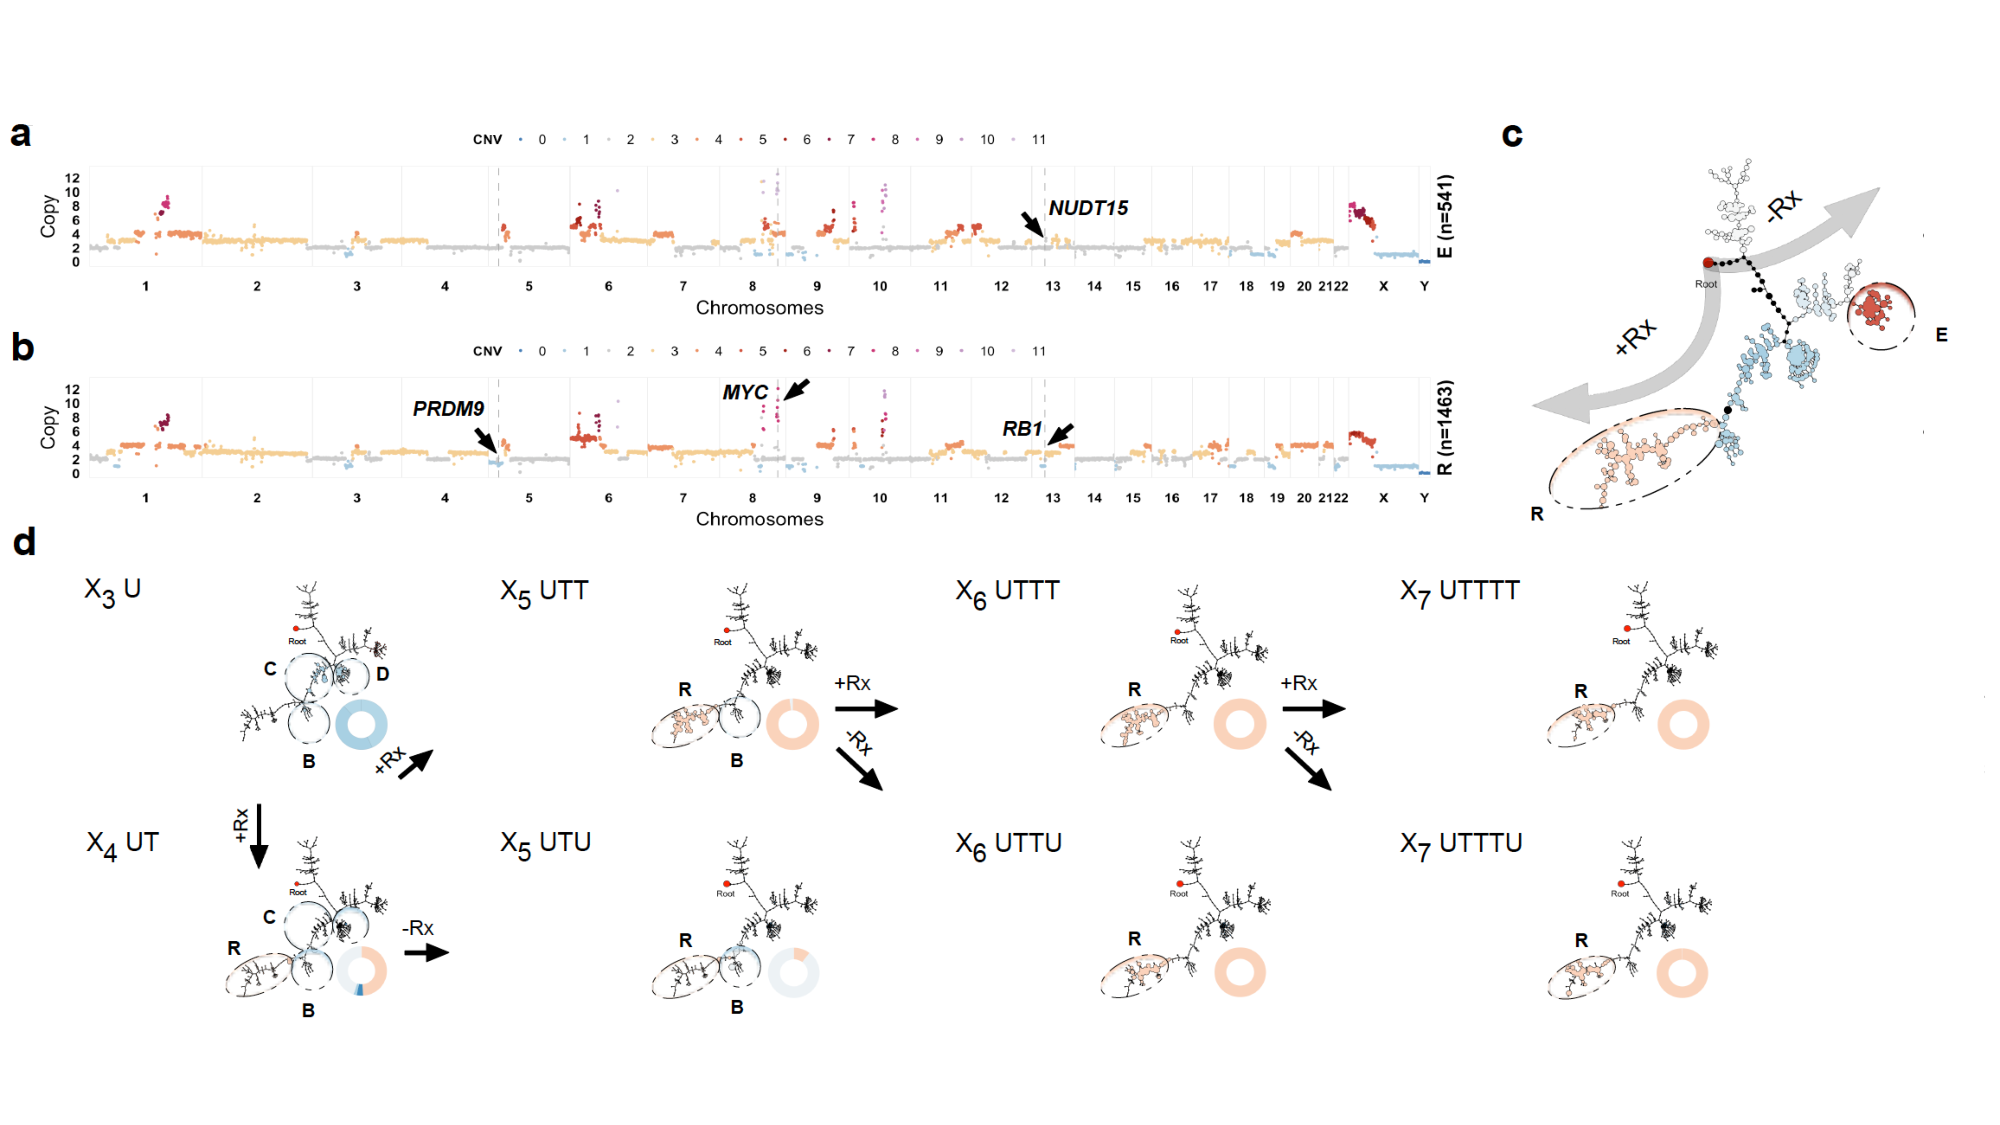
\includegraphics[width=\textwidth]{Figures/drugholidayfitnesscost.pdf}
	
\caption[Impact of cisplatin perturbation on fitness landscape in  SA609 TNBC PDX.]
	{\small
	\textbf{Impact of cisplatin perturbation on fitness landscape in  SA609 TNBC PDX.}
	  \textbf{(a)} Copy number genotype of clone E from untreated timeseries \textbf{(b)} Copy number genotype of clone R from treated timeseries (arrows indicate differences to clone E) \textbf{(c)} Clades with higher fitness in the untreated (-Rx) and treated (+Rx) series \textbf{(d)} Evolution as a function of drug treatment and drug holiday. Arrows indicate the path of serial passaging. For each sample, the phylogeny with clonal abundance from DLP+ is shown, reflecting selection..
	}
	\label{fig:drugholidayfitnesscost}
\end{figure}

%......................................................


\begin{figure}
\centering
\includegraphics[width=\textwidth]{Figures/SA609Rxnew.pdf}
	
\caption[SA609 TNBC PDX clonal dynamics with and without treatment.]
	{\small
	\textbf{SA609 TNBC PDX clonal dynamics with and without treatment.}
	    \textbf{(a)} Heatmap representation of copy number profiles of 841 cells, grouped in 6 phylogenetic clades 
	    \textbf{(b)} Phylogeny (simplified type II sitka tree) of cells over the SA609-Un-Rx where nodes are groups of cells (scaled in size by number) with shared copy number genotype and edges represent distinct genomic copy number change points (sitka markers). \textbf{(c)} Observed clonal abundances \textbf{(d)} distribution over magnitude of difference between selective coefficients of pairs of clones \textbf{(e, f, g, h)} Analogous plots for the treated branch (n=1,593 cells).
	}
	\label{fig:SA609Rxnew}
\end{figure}

%.......................................................


\subsubsection {Clone-specifc cisplatin resistance has a fitness cost}
We next asked whether the clonal dynamics in the presence of cisplatin were reversible by exploring the drug holiday samples \textbf{(\autoref{fig:treatedtimeseriesgreen} a}, \textbf{\autoref{fig:drugholidayfitnesscost} d)} \textit{X5 UTU}; \textit{X6 UTTU}; \textit{X7 UTTTU}). In the first drug holiday \textit{X5 UTU}, clonal composition reverted to consist predominantly of precursor clone B with 90\% abundance, and only 10\% abundance from clone R, \textbf{\autoref{fig:landscapefitness}}.  However, in \textit{X6 UTTU} and \textit{X7 UTTTU} no reversion was detected, and these populations consisted of  $>$99\% Clone R, similar to their on-treatment analogues. Thus, clonal competition in the absence of drug led to clones derived from the A-B clade out-competing clone R, and clone-specific cisplatin resistance thus has a fitness cost. Moreover, the genotype specificity of reversion between \textit{X4 UT} to \textit{X5 UTU} indicates that the clonal dynamics can be attributed to selection of genomically defined clones with differential fitness. 


\subsubsection{Fitness inversion is reproducible and not a stochastic effect}
Next, we examined whether the fitness inversion dynamics as a result of cisplatin chemotherapy in SA609 TNBC PDX model are due to stochastic effect or real.

We established parallel replicate timeseries of SA609 with cisplatin treatment shown as line 2 and line 3 in \textbf{\autoref{fig:treatedtimeseriesgreen} a}, and duplicate experiments of specific time points. We observed the same type of clonal dynamics as of line 1, briefly, a phylogenetic branch of the population which has low fitness in the untreated control branch is repeatedly observed to selectively expand on treatment. The precurosr clone B that gave rise to clone R in line 1, also gave rise to clone R1 in \textbf{\autoref{fig:SA609barplotanalysis} Line 2}. Few time points analysis of line 3 also exhibited expansion of precursor clone B started giving rose to clone R, that was again found to be reversed in drug holiday sample of \textbf{\autoref{fig:SA609barplotanalysis} Line 3}. This indicates that the fitness inversion is not a stochastic effect and establishes with precision that high fitness lineages in the untreated setting are selectively pruned, while low fitness lineages in the untreated setting selectively expand.
%.....................................................................

\begin{figure}
\centering
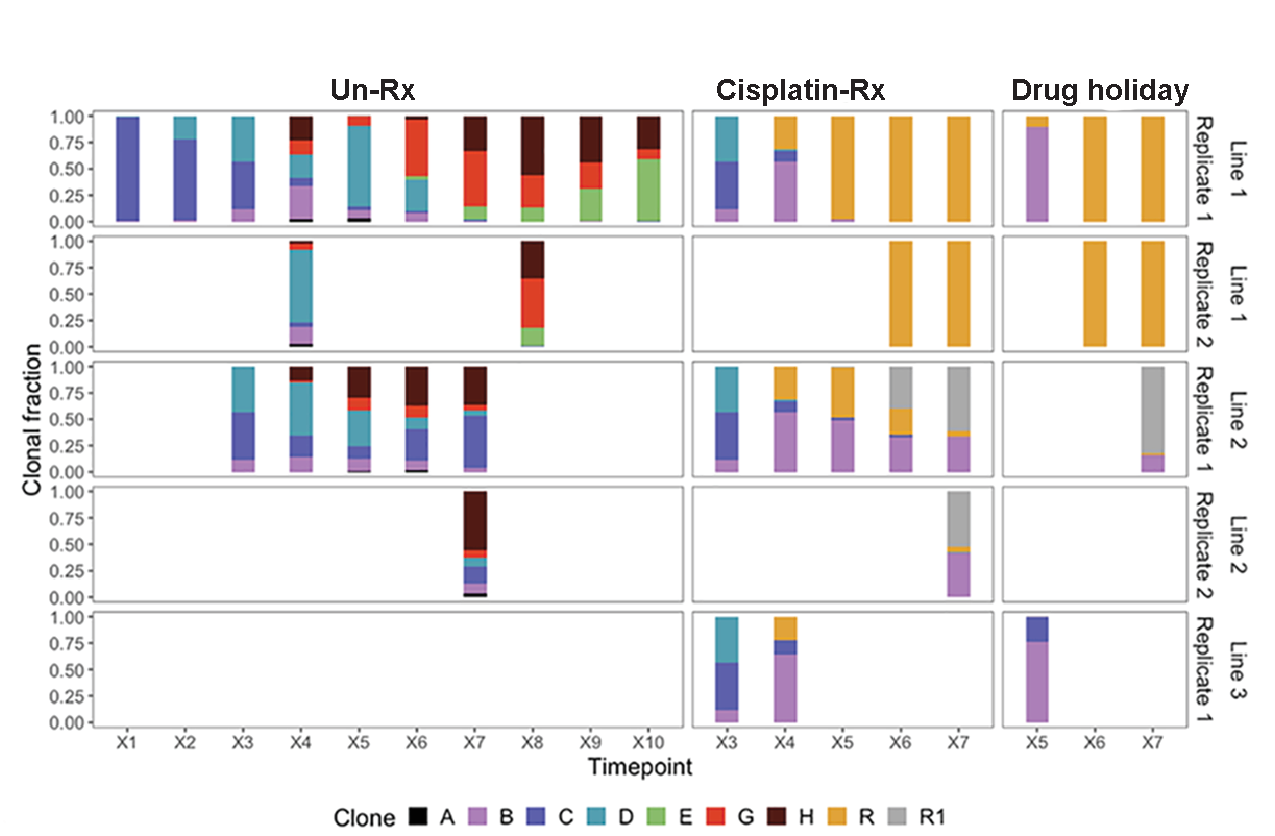
\includegraphics[width=\textwidth]{Figures/SA609barplotanalysis.pdf}
	
\caption[TNBC-SA609 PDX reproducible clonal dynamics with and without treatment]
	{\small
	\textbf{TNBC-SA609 PDX reproducible clonal dynamics with and without treatment.}
	    In both Line 1 and Line 2, the derivatives of clone B (R and R1) sweep the population. Line 3 confirms the same dynamics of clonal proportion with reversal of fitness at X5 in drug holiday sample where clone R is not fit in the absence of drug.
	}
	\label{fig:SA609barplotanalysis}
\end{figure}

%.....................................................................

\subsection{Reversal of fitness landscape is generalizable under cisplatin selective pressure}
To test the generalizability of the observed drug selection dynamics with cisplatin, we performed the same experimental timeseries on two additional TNBC PDX models derived from new patients identified here as SA1035 and SA535 \textbf{\autoref{fig:treatedtimeseriesgreen}  b, c)}. 

\subsubsection{Fitness inversion landscape also observed in SA1035-TNBC PDX with cisplatin}
Another independent PDX system with 14,170 single cells were generated where 4,444 passed the quality filters. The experimental design diagram is shown in \textbf{\autoref{fig:treatedtimeseriesgreen} b}.
Sc-WGS data collected from an untreated branch with five serial passages (X4, X5, X6, X7, and X8) \textbf{\autoref{fig:treatedtimeseriesmanuscript} b)} with a total of 2,015 single cells. A parallel branch was treated with cisplatin starting at X5, X6, X7, and X8 comprising 1,596 filtered cells. 833 cells belonged to the drug-holiday timepoints \textbf{(\autoref{fig:drugholidaysamples} right top panel)}. Phylogenetic inference followed by cutting the tree yielded 11 clones \textbf{(\autoref{fig:SA1035Rxnew}, \autoref{fig:landscapefitness}} . Clonal fractions over all timepoints in the untreated branch were A(0.097), B(0.140), C(0.087), D(0.160), E(0.266), F(0.010), G(0.058), H(0.053), I(0.065), J(0.018), and K(0.047). The abundance of clone A fell over time and it was chosen as the reference clone. Clone E rose from a clonal fraction of 0.028 at X4 to 0.69 at X8 and had the highest selection coefficient (1+s = 1.06 $\pm$ 0.0367). In the treated branch, clonal fractions were A(0.065), B(0.129), C(0.132), D(0.066), E(0.055), F(0.018), G(0.205), H(0.144), I(0.094), J(0.014), and K(0.078). In this regime, G (1+s = 1.01 $\pm$ 0.0123) and H (1+s = 1.02 $\pm$ 0.0135), which were among the clones with lower fitness in absence of treatment, rose to occupy 73\% at X8 while clone E (1 + s = 0.993 $\pm$ 0.0344) fell from about 10\% at X5 to undetectable at X8. Unlike SA609 TNBC, where we saw new clone emerging from existing precursor clone. A clone H with highest fitness coefficient in SA1035 TNBC, was already present in the initial population at the start of drug treatment and in a small proportion in untreated initial samples, but it exponentially increased with drug cycles \textbf{(\autoref{fig:SA1035Rxnew} c, g)}. 

\subsubsection{High fitness clone emerged from the existing starting population with cisplatin in SA535-TNBC PDX}
 SA535 TNBC is a BRCA1 deficient patient derived tumour. We established a timeseries transplants with treated and untreated branches similar to SA609 TNBC PDX \textbf{\autoref{fig:treatedtimeseriesgreen} c}.
 We generated a total of 15,302 single cells out of which 4,023 passed our quality filters.
 We acquired sc-WGS on 5 consecutively transplanted timepoints (X5, X6, X7, X8, X9) left untreated \textbf{(\autoref{fig:treatedtimeseriesmanuscript} b)} for a total of 1,341 single cells (mean = 335, $\sigma$ = 84.4 per timepoint). Simultaneously, we established a cisplatin treated timeseries starting from timepoint X6, and continued cisplatin treatment for 5 cycles up to X10, generating a total of 1,425 cells from scWGS (mean = 356, $\sigma$ = 159 per timepoint) from 4 cycles. A cut of the phylogenetic tree inferred over all cells in this series, resulted in 7 clones. In the untreated line, clonal fractions were A(0.003), B(0.702), C(0.034), D(0.006), E(0.006), F(0.013), and G(0.237).
Clone B was chosen as the reference clone as it had a monotonically decreasing clonal fraction trajectory in the untreated branch. Clonal trajectories were consistent with selection coefficients
with small relative differences in fitness \textbf{\autoref{fig:SA535analysis} d)}. Clone G had the highest fitness (1 + s = 1.01 $\pm$ 0.00751) closely followed by clone C (1+s = 1.00 $\pm$ 0.0282) and the reference clone. In the treated branch, clonal fractions were A(0.156), B(0.066), C(0.140), D(0.194), E(0.182), F(0.151), and G(0.112). In this regime, clone A emerged with the highest selection coefficient (1 + s = 1.03 $\pm$  0.0152) followed by clone D (1 + s = 1.02 $\pm$ 0.0116). Notably clones A and D had low fitness values under no treatment, whereas clones G (1+s = 1.01 $\pm$ 0.0115) and C (1+s = 1.02 $\pm$ 0.0119) had low fitness coefficients under treatment. Like SA1035 clonal dynamics, SA535 also displayed high fitness clone H emerging from already present initial population,  taking survival advantage under drug selection.

%.................................................................


\begin{figure}
\centering
\includegraphics[width=\textwidth]{Figures/SA1035Rxnew.png}
	
\caption[SA1035 TNBC PDX timeseries clonal dynamics under drug perturbation]
	{\small
	\textbf{SA1035 TNBC PDX timeseries clonal dynamics under drug perturbation.}
	    \textbf{(a)} Heatmap representation of copy number profiles of
2,015 cells, grouped in 11 phylogenetic clades  \textbf{(b)}Phylogeny (simplified type II sitka tree) of cells over the SA1035-Un-Rx where nodes are groups of cells (scaled in size by number) with shared copy number genotype and edges represent distinct genomic copy number change points (sitka markers). \textbf{(c)} Observed clonal abundances \textbf{(d)} distribution over magnitude of difference between selective coefficients of pairs of clones \textbf{(e, f, g, h)} Analogous plots for the treated branch (n=1,596 cells).
	}
	\label{fig:SA1035Rxnew}
\end{figure}


%.....................................................................

\begin{figure}
\centering
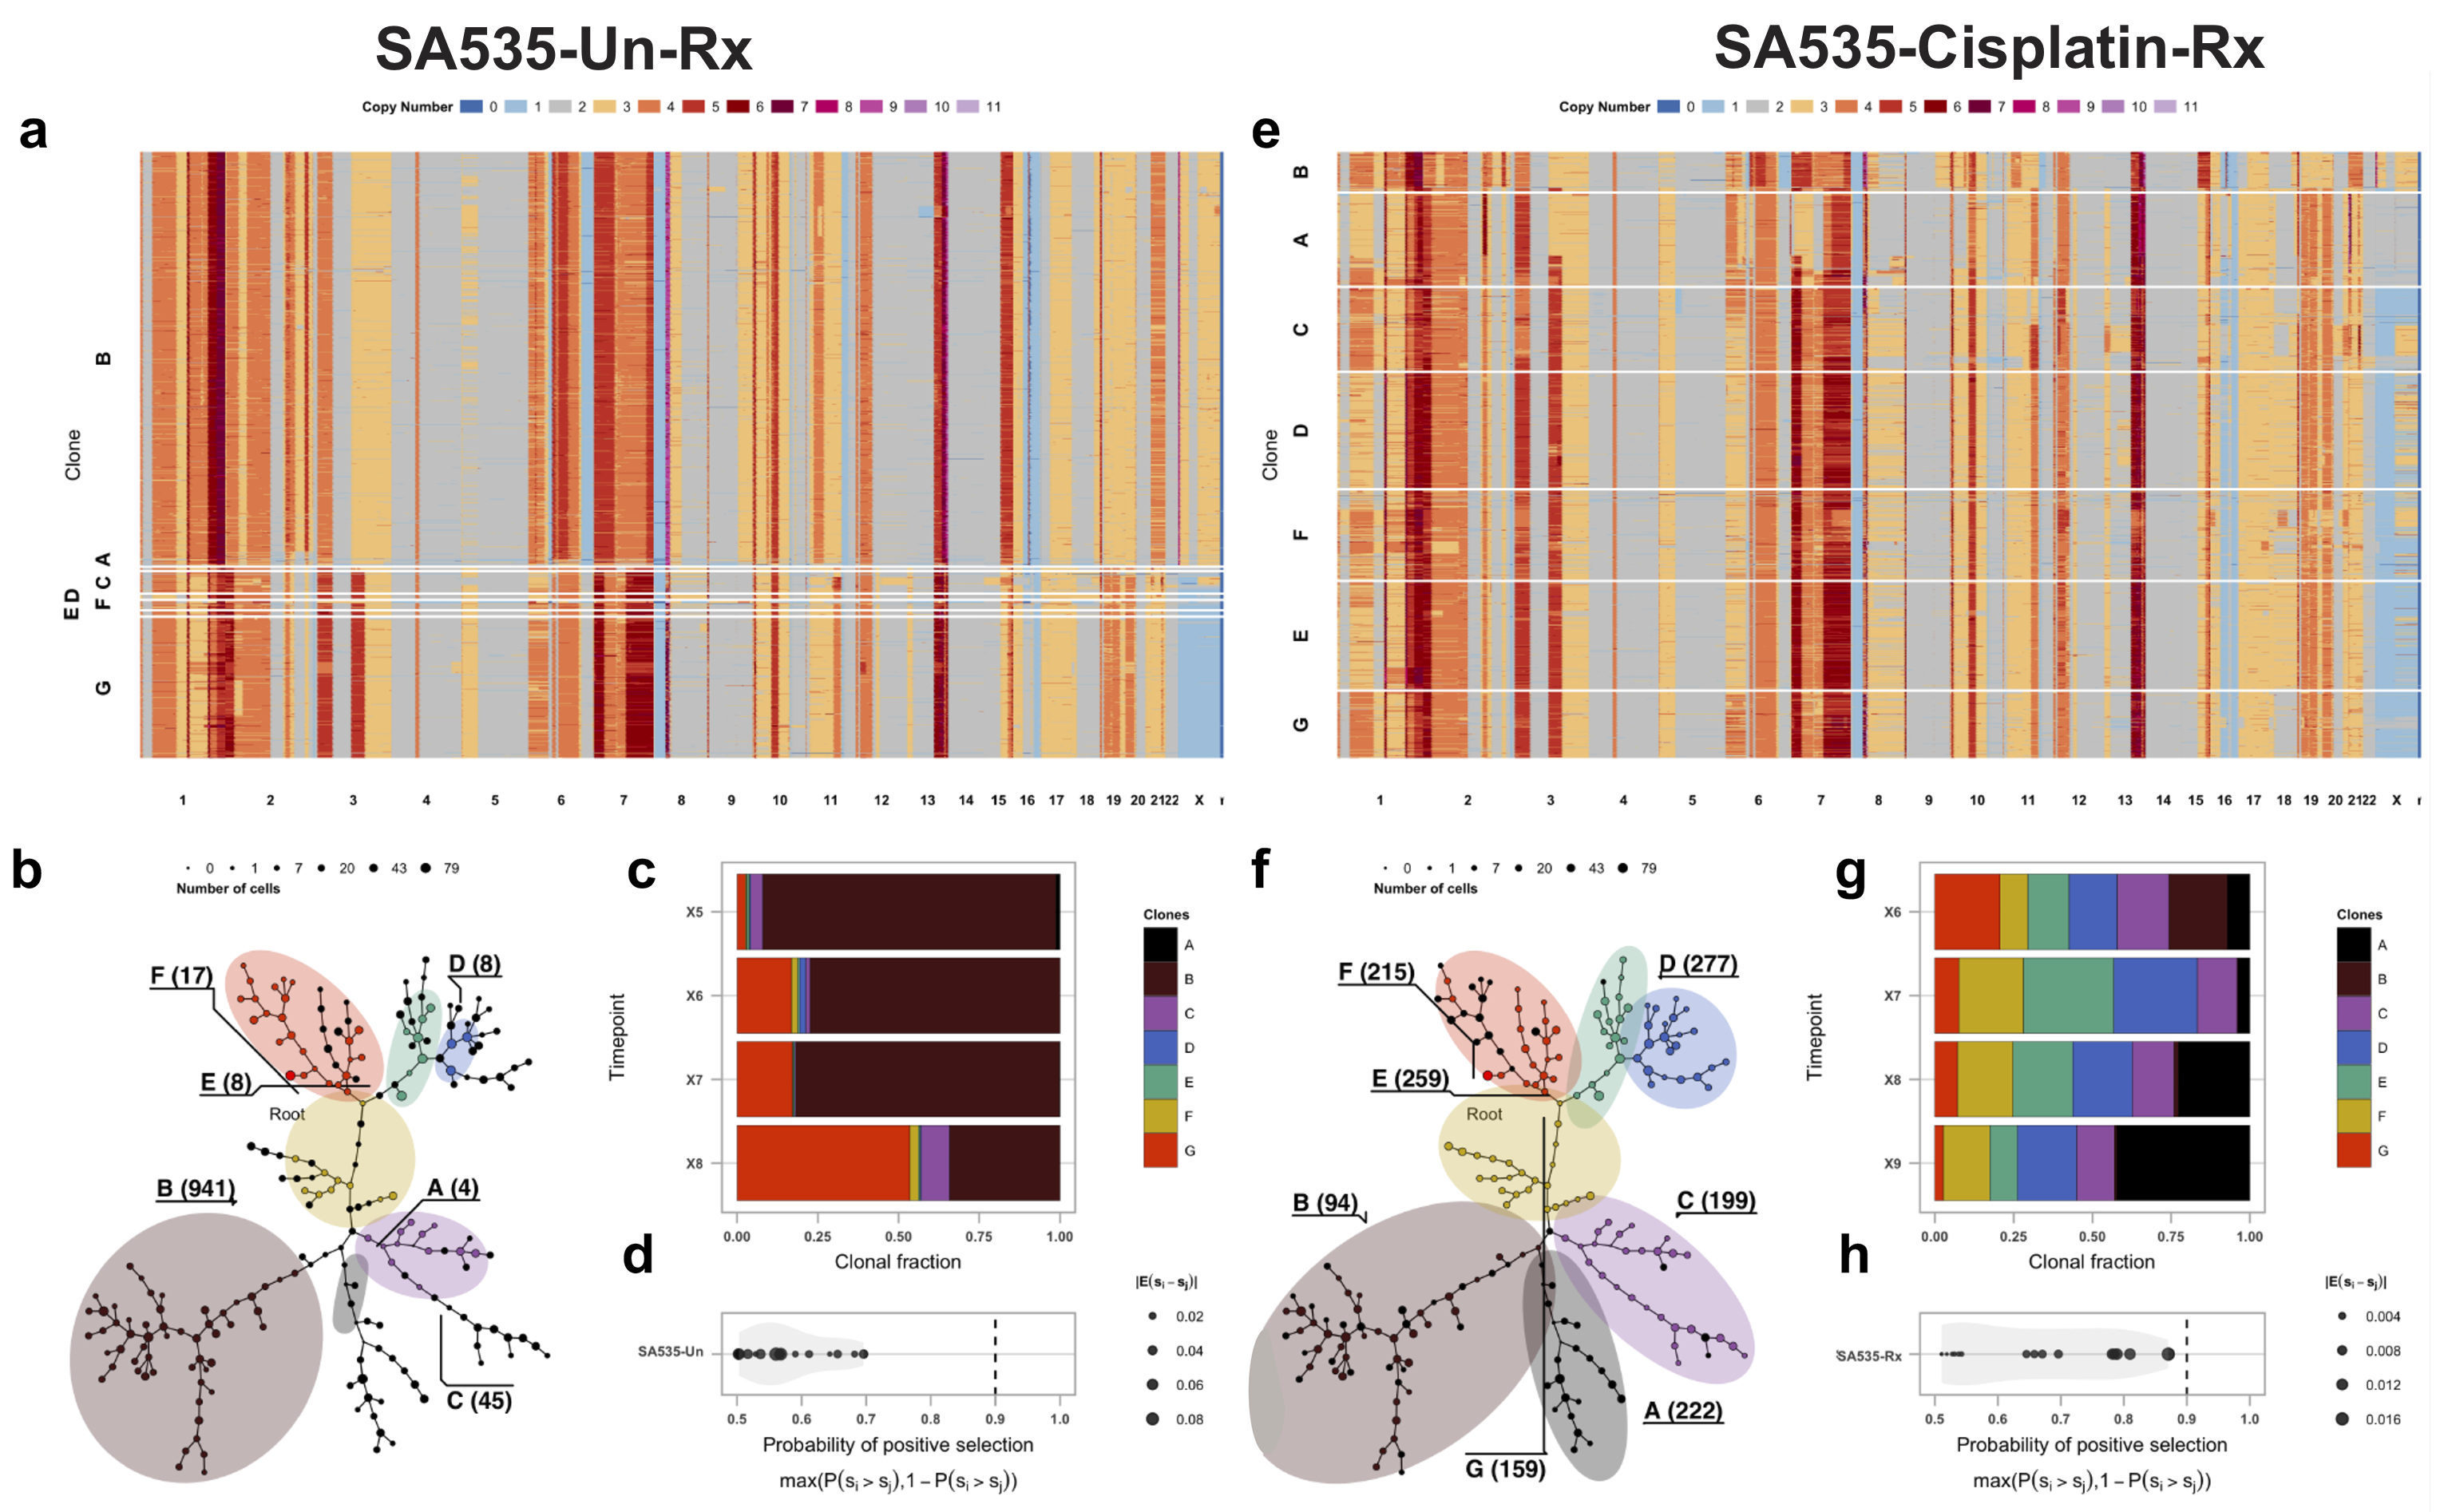
\includegraphics[width=\textwidth]{Figures/SA535analysis.png}
	
\caption[SA535 TNBC PDX timeseries clonal dynamics under drug perturbations]
	{\small
	\textbf{SA535 TNBC PDX timeseries clonal dynamics under drug perturbations.}
	     \textbf{(a)} Heatmap representation of copy number profiles of
2,015 cells, grouped in 11 phylogenetic clades  \textbf{(b)} Phylogeny (simplified type II sitka tree) of cells over the SA535-Un-Rx where nodes are groups of cells (scaled in size by number) with shared copy number genotype and edges represent distinct genomic copy number change points (sitka markers). \textbf{(c)} Observed clonal abundances \textbf{(d)} distribution over magnitude of difference between selective coefficients of pairs of clones \textbf{(e, f, g, h)} Analogous plots for the treated branch (n=1,425 cells).
	}
	\label{fig:SA535analysis}
\end{figure}

%...............................................................

\begin{figure}
\centering
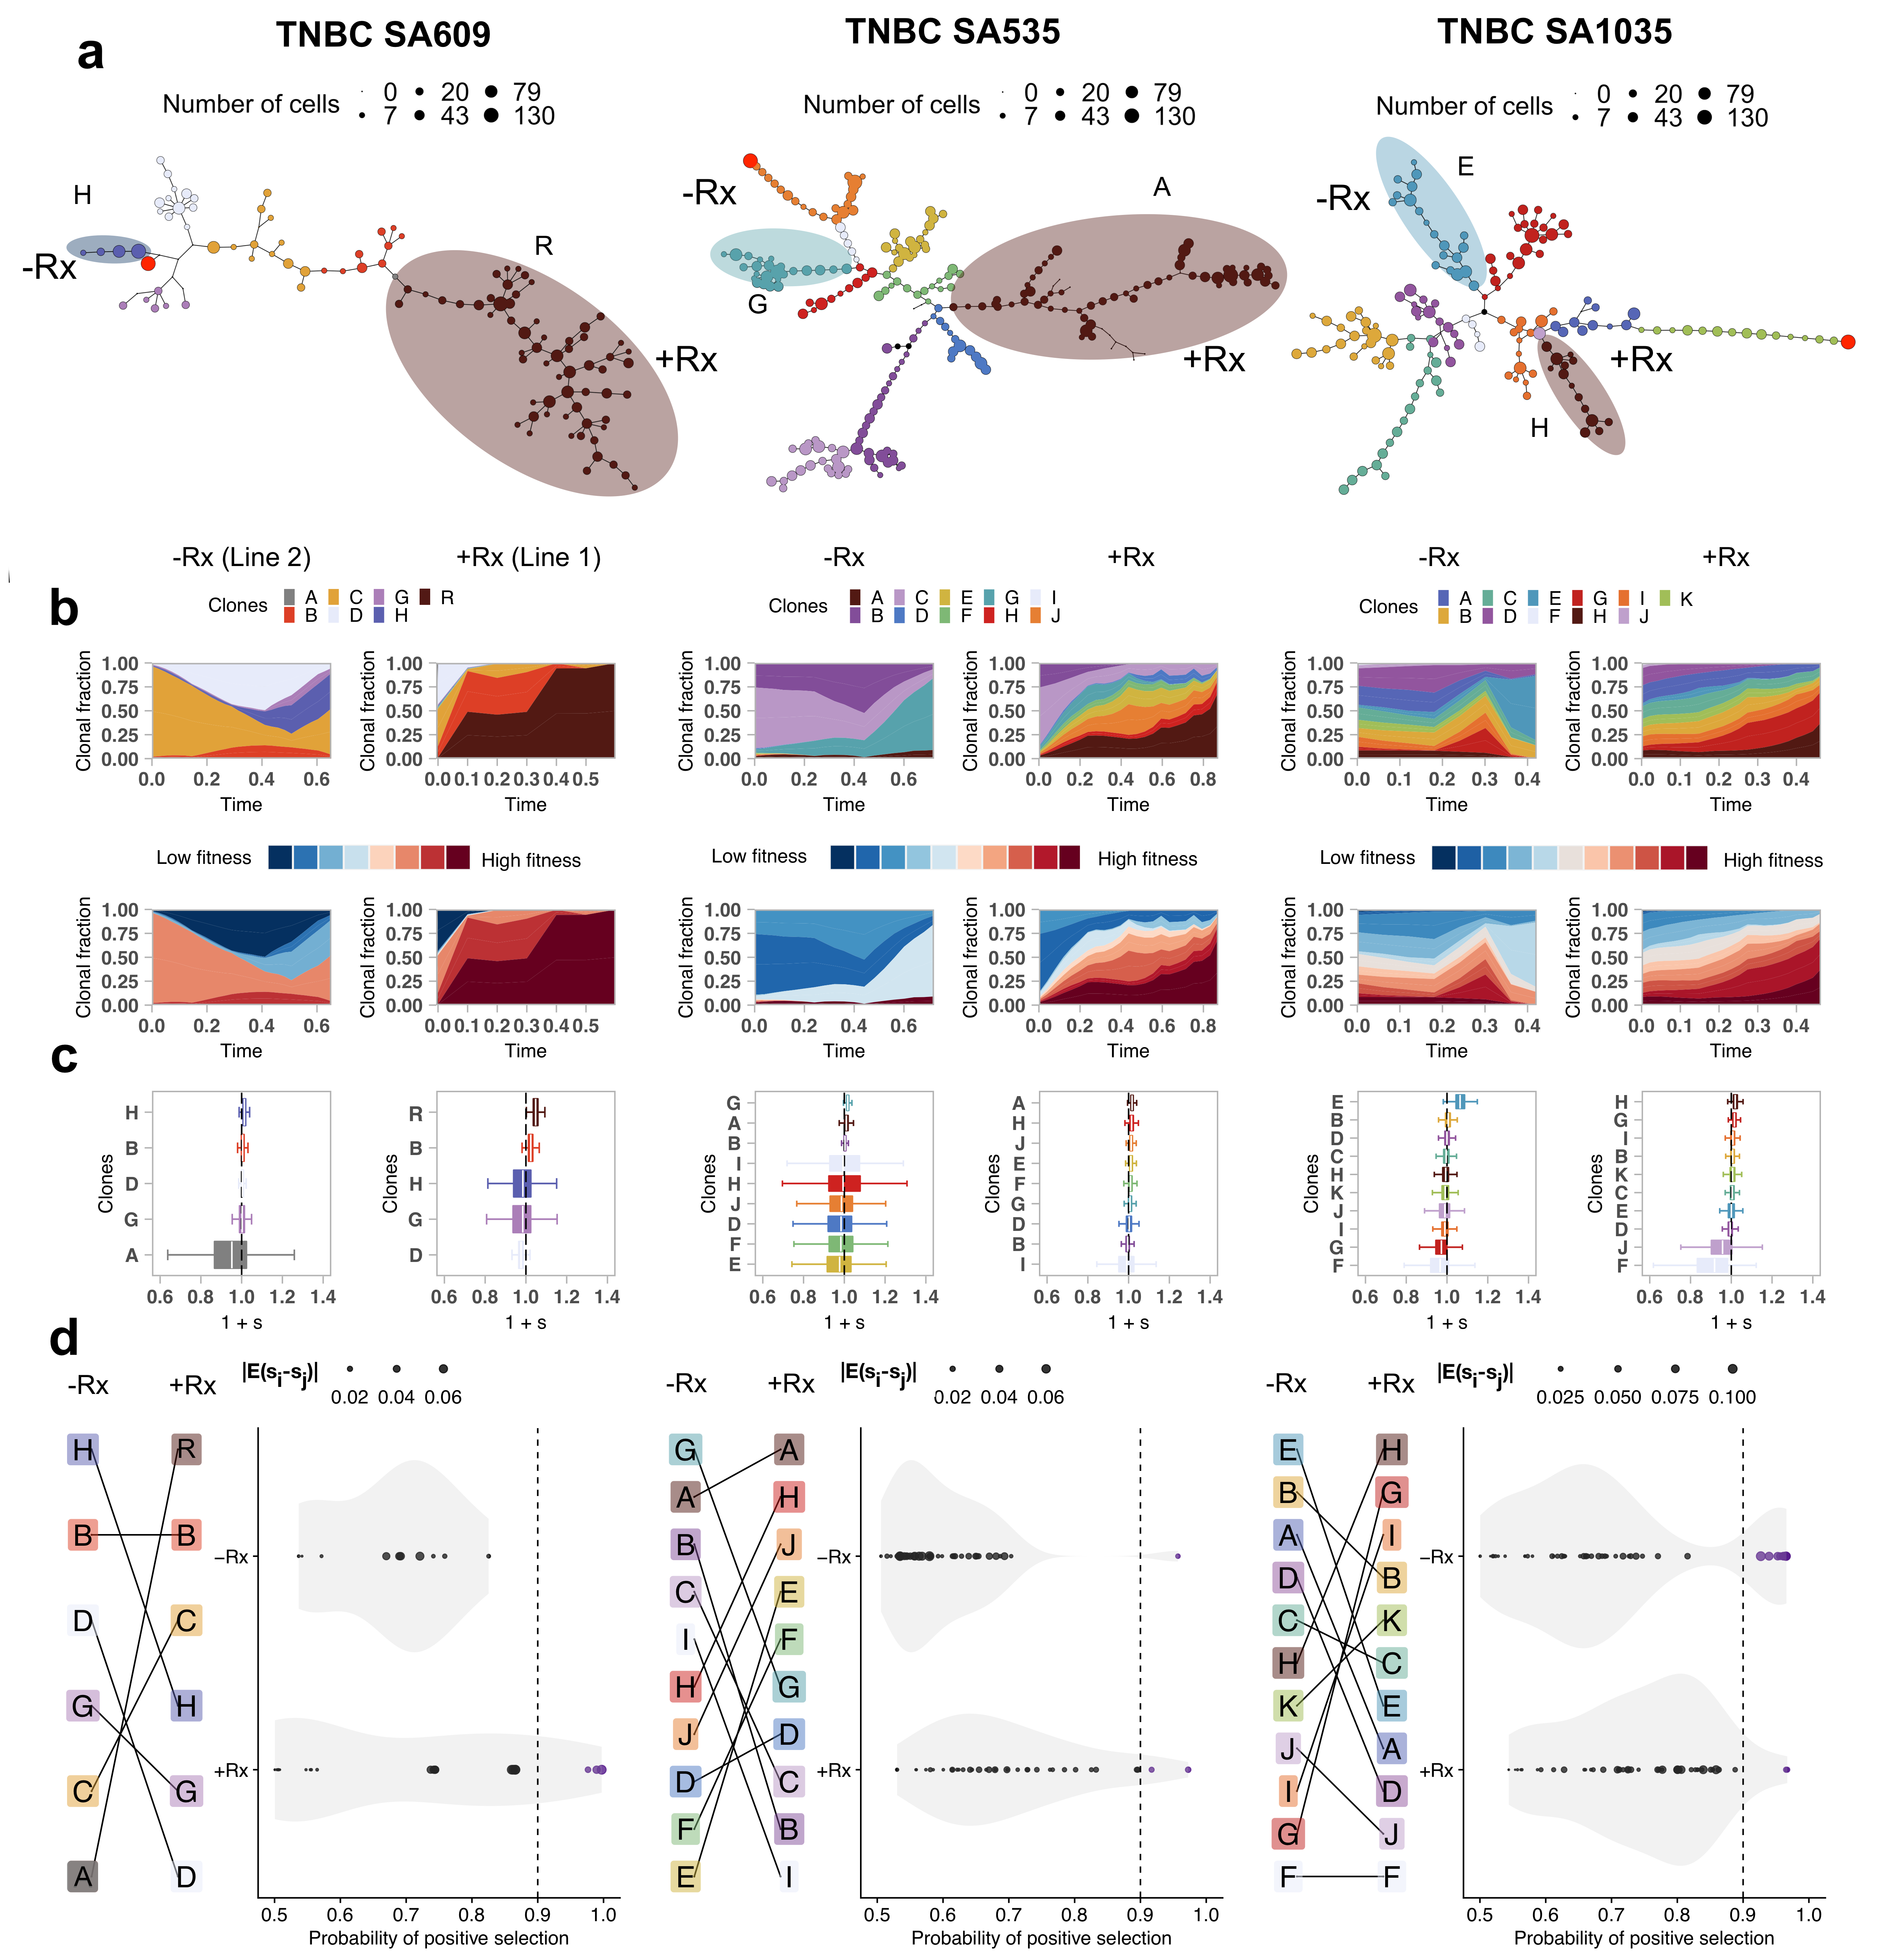
\includegraphics[width=\textwidth]{Figures/landscapefitness.png}
	
\caption[Fitness landscape reversal in early cisplatin treatment in TNBC PDX models.]
	{\small
	\textbf{TNBC PDX models exhibiting fitness landscape inversion in early cisplatin treatment.}
	     We observe in 3 independent TNBC PDX lines that clone specific resistance to cisplatin treatment arises. In all three cases, clones with low fitness under no treatment exhibit high fitness under the treatment regime. In each panel, the left and right sub-panels are from the untreated and treated branches respectively \textbf{(top)} Phylogenetic trees showing clones sorted by their median selection coefficient in -Rx and +Rx regimes  \textbf{(middle)} inferred trajectories, and  \textbf{(bottom)} selection coefficients of \texttt{fitClone} model fits to each branch.
	}
	\label{fig:landscapefitness}
\end{figure}
%.....................................................................


\subsubsection{Fitness inversion summary from TNBC under cisplatin regime }
In the TNBC-SA609 system the fitness landscape is inverted wherein
clones more fit in the untreated regime (H, D) are less fit in the treated regime, whereas less fit clones in the untreated regime (A, B) are the most fit clones under treatment. This pattern is
mirrored in two independent TNBC PDX lines treated with cisplatin, namely TNBC-SA535 and TNBC-SA1035. In TNBC-SA535, clones G, C, and B are drug-sensitive, meaning they could not survive drug pressure, while A and D are drug resistant because they are showing high fitness coefficient in the presence of drug. Also,the former have higher relative fitness in untreated versus treated regimes, while the latter exhibit an inverted fitness pattern. Similarly, in TNBC-SA1035, drug-sensitive clones consist of clones E, B, and A, while the drug-resistant group comprises clones H, I, and G. From untreated
to treated, the first group goes from high to low fitness, while the second group goes from low to high fitness. \textbf{\autoref{fig:landscapefitness}} summarises the reversal in the fitness landscape in response to cisplatin treatment in TNBC-PDX model systems.

%...........................................................


\subsection{Comparison of fitness landscape of platinum and CX-5461 in TNBC PDX timeseries}
So far we have applied only platinum compound to TNBC PDX in a time series manner to track copy number based genomic clones. Now we investigate whether establishing the same patients tumor model of forced amplified evolution, with another drug, CX-5461, could help to interpret the clonal relationship and their fitness within the same tumor type.
One TNBC SA535, was BRCA1 deficient (HRD-Dup), so we developed a repeated CX-5461 drug exposure timeseries model same experimental design \textbf{(\autoref{fig:SA535CX5461} a)} to compare cisplatin induced clonal dynamics. Platinum (cisplatin) is a standard chemotherapeutic agent whereas, CX-5461 is a G4 quadruplex stabilizer drug, known to have synthetic lethality with BRCA deficiency.

We established a timeseries SA535 TNBC PDX treated and untreated branches of CX-5461 similar and in parallel to cisplatin.
we established a CX-5461 treated timeseries starting from timepoint X5 to X9 while cisplatin continued in parallel from X6 to X10  \textbf{\autoref{fig:SA535CX5461} a}. Another untreated timeseries simultaneously was set up for comparison of dynamics and tumor growth rate record.
We collected sc-WGS from consecutively transplanted treated and untreated all aforementioned timepoints for a raw total of 44,618 single cells (mean = 1274.8, $\sigma$ = 300.8 per library. After aggressive filtering for a very high quality human genomes and removing dividing cells, we analysed a total of 7,894 (mean = 1127.7, $\sigma$ = 708.2 per timepoint) single cells from the whole SA535 TNBC PDX \textbf{(\autoref{fig:SA535combinebarplots} a)}

We acquired scWGS on 7 consecutively transplanted untreated timepoints (X4, X5, X6, X7, X8, X9, X10) generating a total of 1,968 single cells (mean = 328, $\sigma$ = 104.5 per timepoint).
Clonal fractions calculated as I(0.002), J(0.3206), K(0.0071), L(0.0051), N(0.0066), P(0.0056), Q(0.6011), R(0.0386), S(0.0097), U(0.0036). 

Simultaneously,from a Cisplatin treated timeseries starting from timepoint X6, and continued for 5 cycles up to X10, generating a total of 2,921 cells from scWGS (mean = 584.2, $\sigma$ = 190.5 per timepoint) from 5 cycles. A cut of the phylogenetic tree inferred over all cells in this series, resulted in 13 clones.
In the drug cycle treatment Cisplatin line, clonal fractions were
calculated as I(0.1568), J(0.0575), K(0.0791), L(0.1852), N(0.0065), O(0.001), P(0.1072), Q(0.0387), R(0.0524), S(0.0839), T(0.1938) and U(0.038).

Moreover, from a CX-5461 treated timeseries, starting from timepoint X5, and continuing for 5 cycles up to X9, we generated a total of 3,005 cells from scWGS (mean = 601, $\sigma$ = 342 per timepoint). A cut of the phylogenetic tree inferred over all cells in this series, resulted in 13 clones. In the drug cycle treatment CX-5461 line, clonal fractions were I(0.0004), J(0.0077), K(0.0027), L(0.0013), M(0.0389), N(0.0709),  O(0.0795), P(0.003), Q(0.005), R(0.3428), S(0.016), U(0.4319).
Tumor growth curves displayed progressively less response of the tumors in last cycle of drug as compared to the first, indicating initiation of drug resistance to both cisplatin and CX-5461 \textbf{(\autoref{fig:SA535CX5461} b, c)}. Positive growth kinetics started earlier in cisplatin tumors as compared to CX-5461.
%......................................................

\begin{figure}
\centering
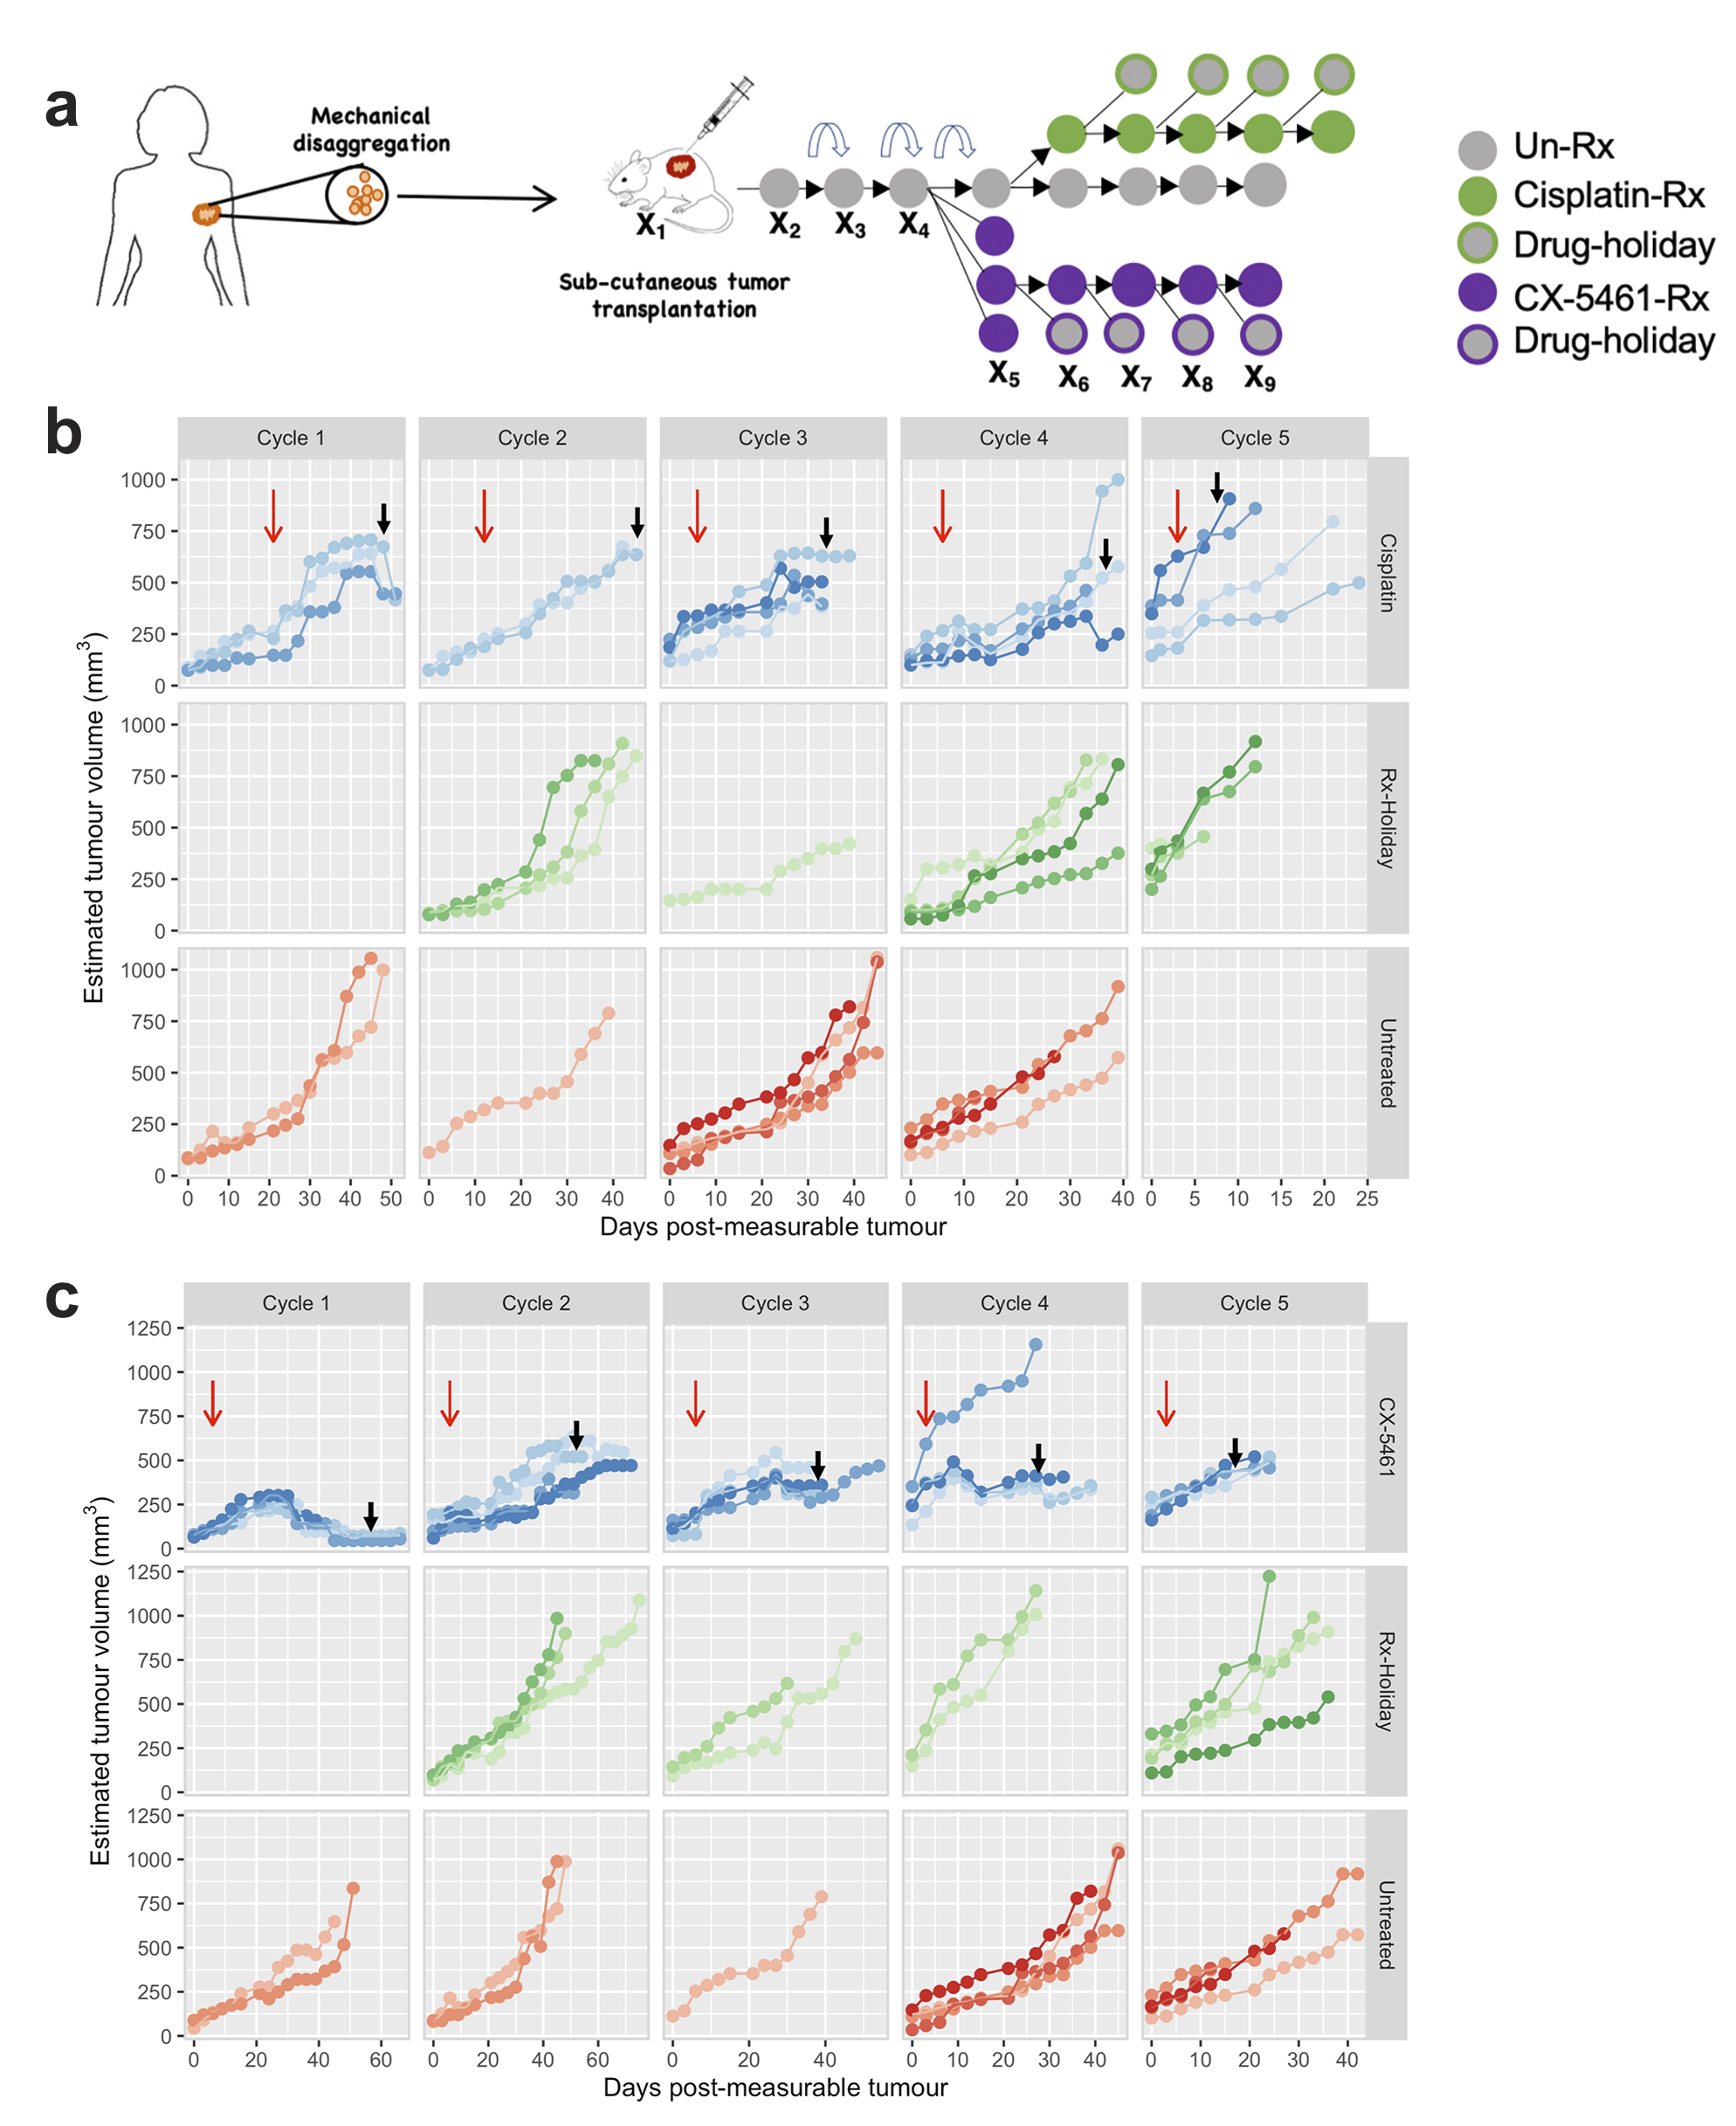
\includegraphics[width=\textwidth]{Figures/SA535CX5461 .png}
	
\caption[SA535 TNBC PDX timeseries with cisplatin and CX-5461]
	{\small
 \textbf{SA535 TNBC PDX timeseries with cisplatin and CX-5461.}
Vertical axis on right indicates the tumor status. The top bar gives cycle numbers and left vertical axis gives tumor measurements. Horizontal axis are days post measurable tumors\textbf{(a)} Experimental overview and passaging details of start and end of cisplatin and CX-5461 treatments. Red arrows point to the start of treatemnt and black arrows point to the tumor rdigested for sc-WGS.
	   \textbf{(b)} Growth curves of cisplatin treated tumors
	    \textbf{(c)} Growth curves of CX-5461 treated tumors.
	}
	\label{fig:SA535CX5461}
\end{figure}

%......................................................................



\begin{figure}
\centering
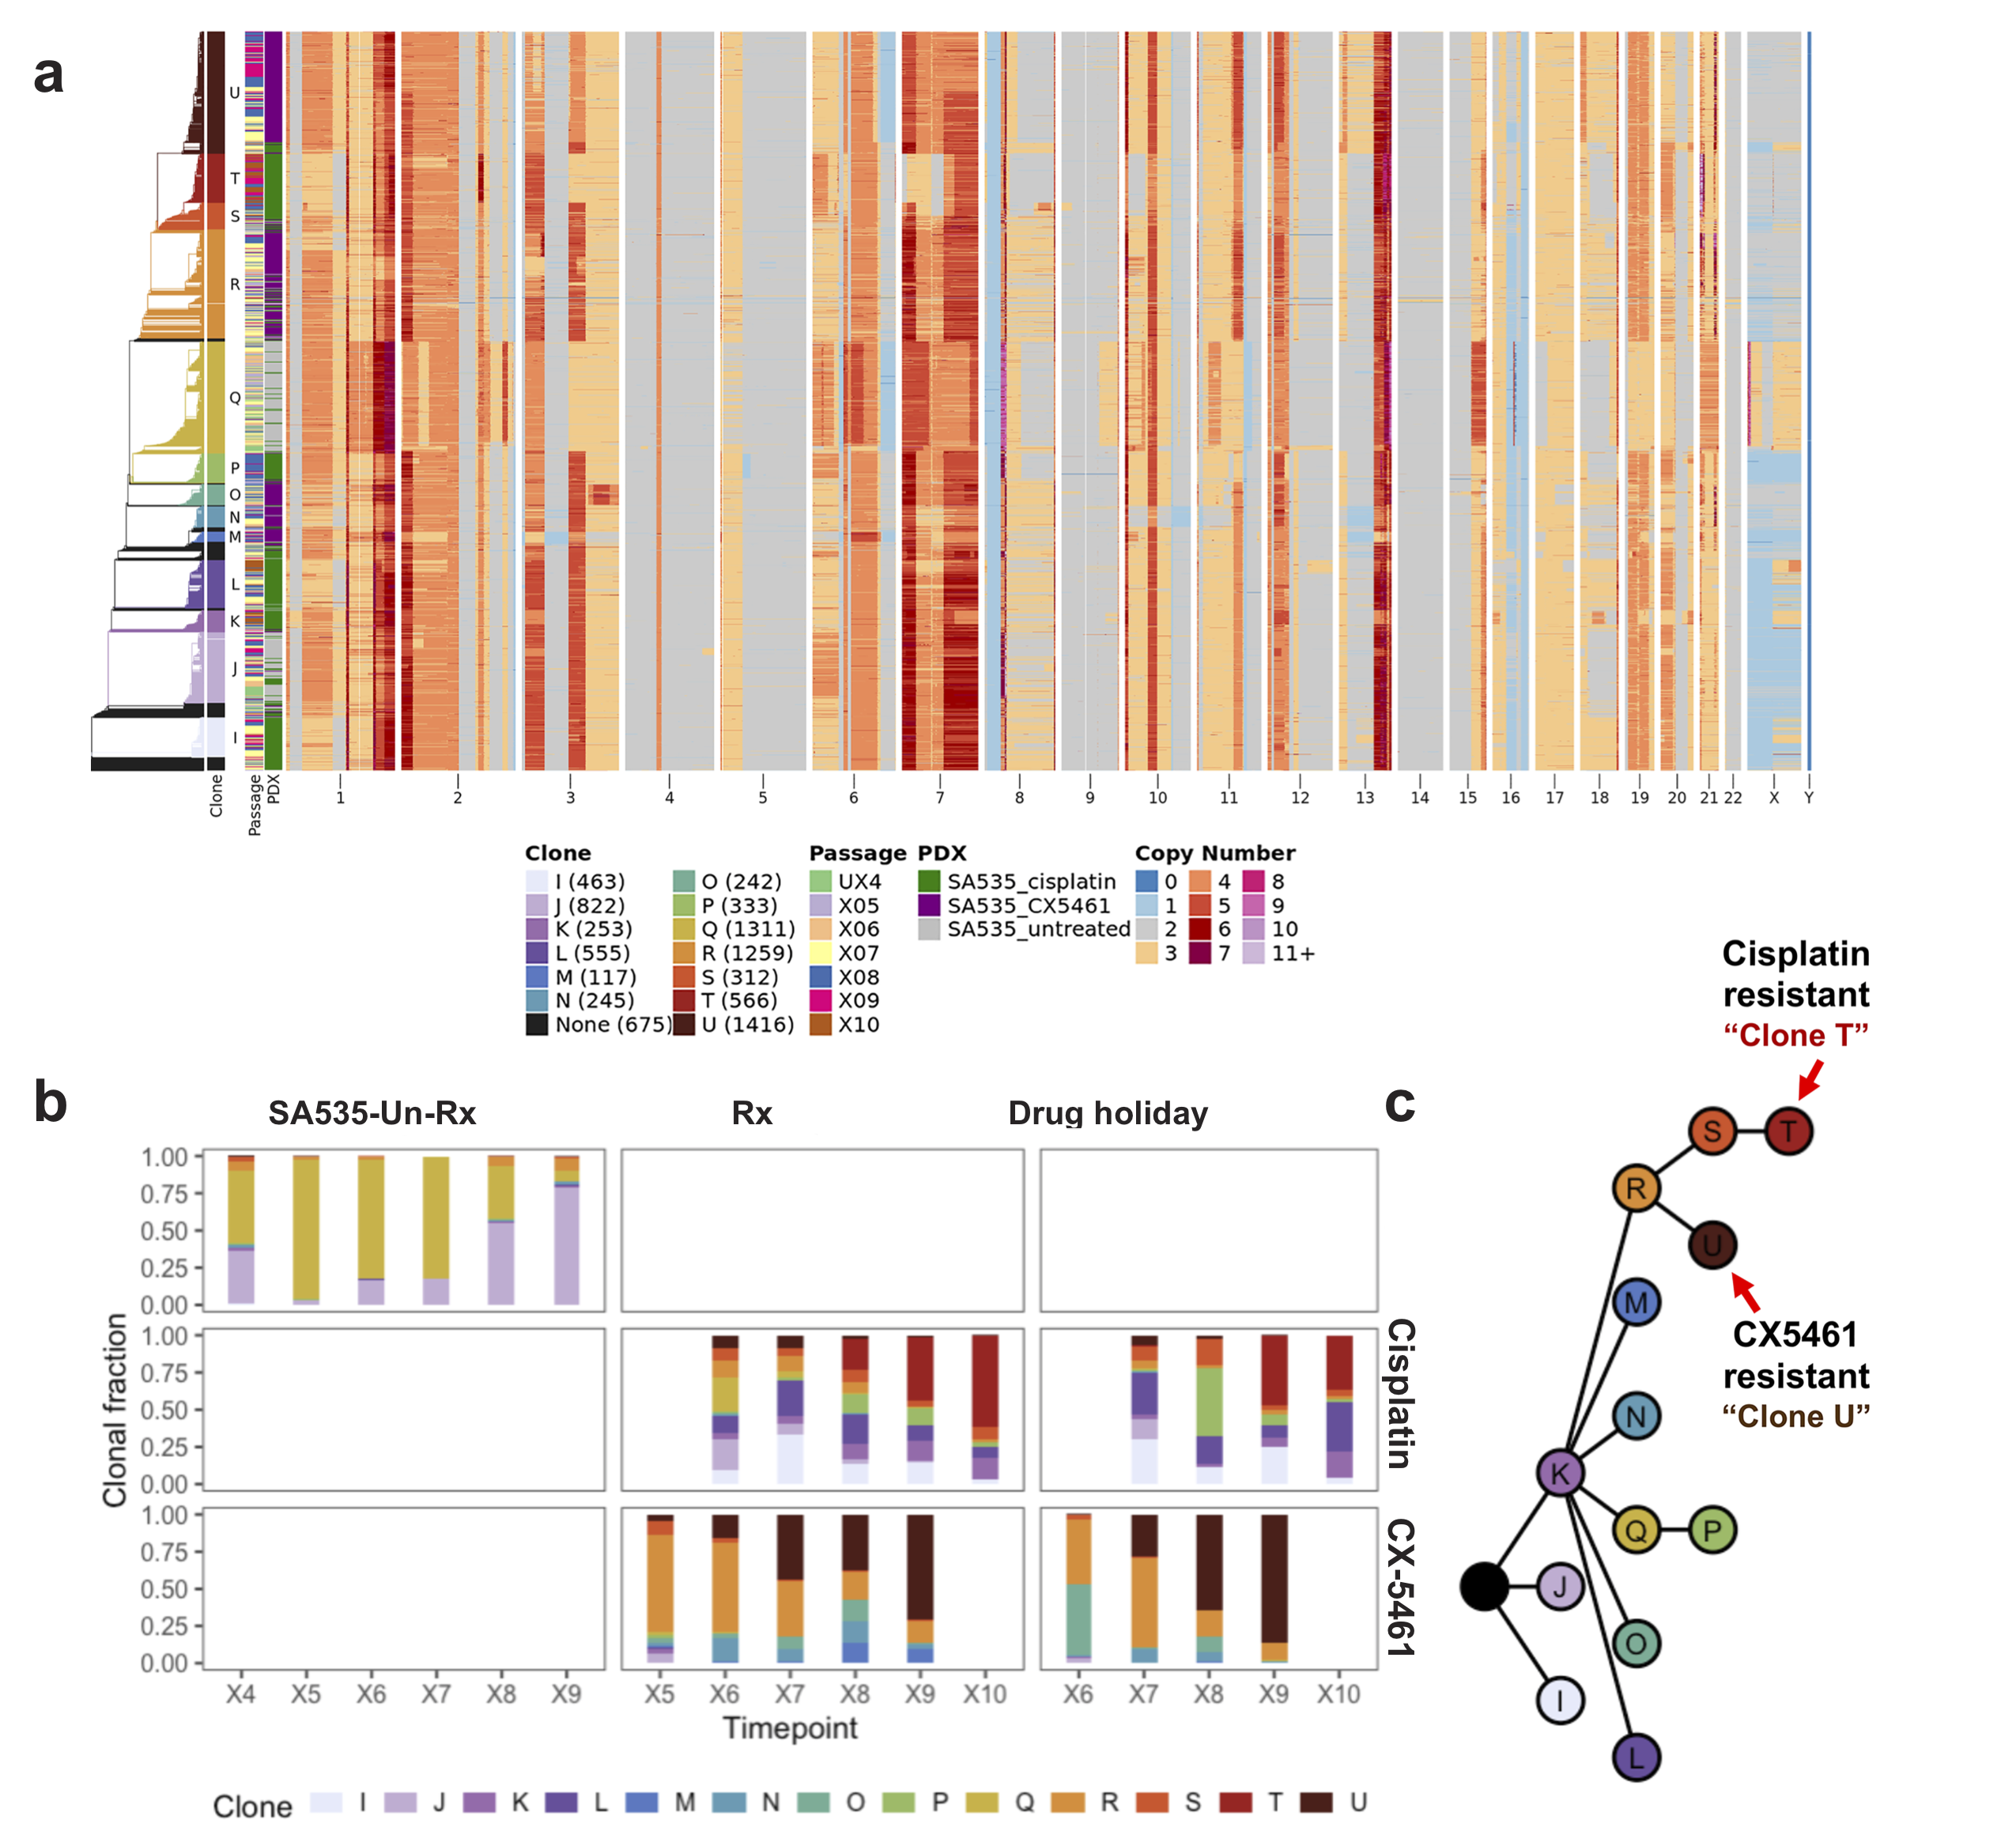
\includegraphics[width=\textwidth]{Figures/SA535combinebarplots .png}
	
\caption[Combined data analysis of SA535 with cisplatin and CX-5461]
	{\small
	\textbf{Combined data analysis of SA535 with cisplatin and CX-5461.}
	   \textbf{(a)} Integer copy number heat map showing vertical columns as chromosomes and each row represent single cell. Red arrows pointing to change in copy number events in that specific clone.
	    \textbf{(b)} Bar plots showing clonal composition at each time point. Vertical axis shows the clonal fraction   and horizontal axis presents the passage timepoint.
	     \textbf{(c)} Simplified way to present clonal lineage tree matching the bars composition in \textbf{(a)}.
	}
	\label{fig:SA535combinebarplots}
\end{figure}

%...............................................................

\subsubsection{Drug resistant clones arise from the same precursor}
Integer heat map of copy number heterogeneity was computed using \texttt{sitka} and interestingly cisplatin and CX-5461 treated cells clustered independently from each other and from the un treated cell clusters \textbf{\autoref{fig:SA535combinebarplots} a}. Clonal abundance for the un treated time series depicted increase of Clone Q till passage 7 (X7) but then gradual decrease favouring emerging of clone J in the later generations \textbf{(\autoref{fig:SA535combinebarplots} b (left top panel))}. In cisplatin treated series, clone T showed up expanding under the drug whereas with CX-5461 favored emerging of clone U.
Moreover, the resistant branches having clone S and clone T for cisplatin and clone U for CX-5461, both derive from clone R, which is present early in variable proportions in the two branches, but does not have fitness in the untreated, present but at a very minor proportion. Perhaps its giving an idea that independently, drug resistance has apparently a favored clonal starting point in this PDX \textbf{\autoref{fig:SA535combinebarplots} c}. 

Comparing drug holiday samples from cisplatin and CX-5461 treated time series informed resistant clones are reversible early in the treatment of cisplatin but not in case of CX-5461 \textbf{\autoref{fig:SA535combinebarplots} b (middle and right panels)}
These results require further confirmation by treating more TNBC PDX with CX-5461.



\section{Discussion}
The fitness landscapes are inverted as a result of cisplatin chemotherapy in  triple negative breast cancer PDX models.  We have generated replicate observations in PDX models in two ways: parallel replicate timeseries transplants with cisplatin treatment, and duplicate experiments of specific time points \textbf{\autoref{fig:treatedtimeseriesgreen} a} . In untreated timeseries \textbf{\autoref{fig:SA609barplotanalysis} left panel}, we observe repeated expansion of clone H, relative to lower fitness clones (e.g. clone D). Furthermore, in treated series, we observe the same clonal dynamics - namely that a phylogenetic branch of the population which has low fitness in the untreated control branch is repeatedly observed to selectively expand on treatment.  Notably, we remark in triplicate lines,  highly congruent dynamics with the introduction of treatment between X3 and X4. 

SA609 TNBC drug holiday data suggest the impact of cisplatin selective pressure on the starting tumour cell population is reversible while genomic clonal competition with precursor clones is still possible, but dominates the population once the evolutionary bottleneck narrows and purifies the population.

Furthermore within lines, we observe through duplicate samplings that the clonal expansion patterns are repeatedly observed. With these repeat experiments, we note that the starting population structure is not deterministic of clonal abundance of future population structure.  We attest that while stochastic effects of sampling cannot be ruled out, the monotonic trajectories of clones and repeated observations strongly suggest variation in fitness as a primary determinant. In additional two series other than SA609 TNBC series, we noted that the starting point of treatment experiments harbours a more balanced representation of high and low fitness clones, and therefore are less subject to the sampling bias.  In the last two series, similar inversions of the fitness landscape are observed.  Together, the replicate experiments and addition of 2 new TNBC PDX series indicate that the fitness inversion is not a stochastic effect and establishes with precision that high fitness lineages in the untreated setting are selectively pruned, while low fitness lineages in the untreated setting selectively expand. The observation that drug resistance can have a fitness cost also points to an underlying mechanism of retained sensitivity in early treatment.






{\chapter{Characterization of cancer transcriptomics under drug perturbations in TNBC-PDX}

}
 \label{ch:Chapter5}
 \section{Motivation}

In spite of advanced technologies and treatment, triple negative breast cancer still facing the problems of tumor recurrence and drug resistance.
For any given difference between the types of drug resistance, for example, the expression of a particular gene, it is assumed that differences arise deterministically or probabilistically in the configuration of transcription factors regulating the genes in the tumors. Cancer cells in distinct cell- states often exhibit important differences in functional properties depending on the which genes are turned on and off resulting in sensitive or resistant phenotype.

The most challenging analysis is to differentiate whether the change in gene expression leading to change in cellular state is stochastic\cite{raj2008nature} and random or its deterministic to produce the same output under similar environment.
Cancer cells in distinct cell- states often exhibit important differences in functional properties depending on which genes are turned on and off resulting in sensitive  or resistant phenotype.
Previously it is shown that unique cells within a population can exhibit fluctuations in expression of a group of genes, that could predict distinct phenotypes \cite{shaffer2019memory}.


\begin{figure}
\centering
  
  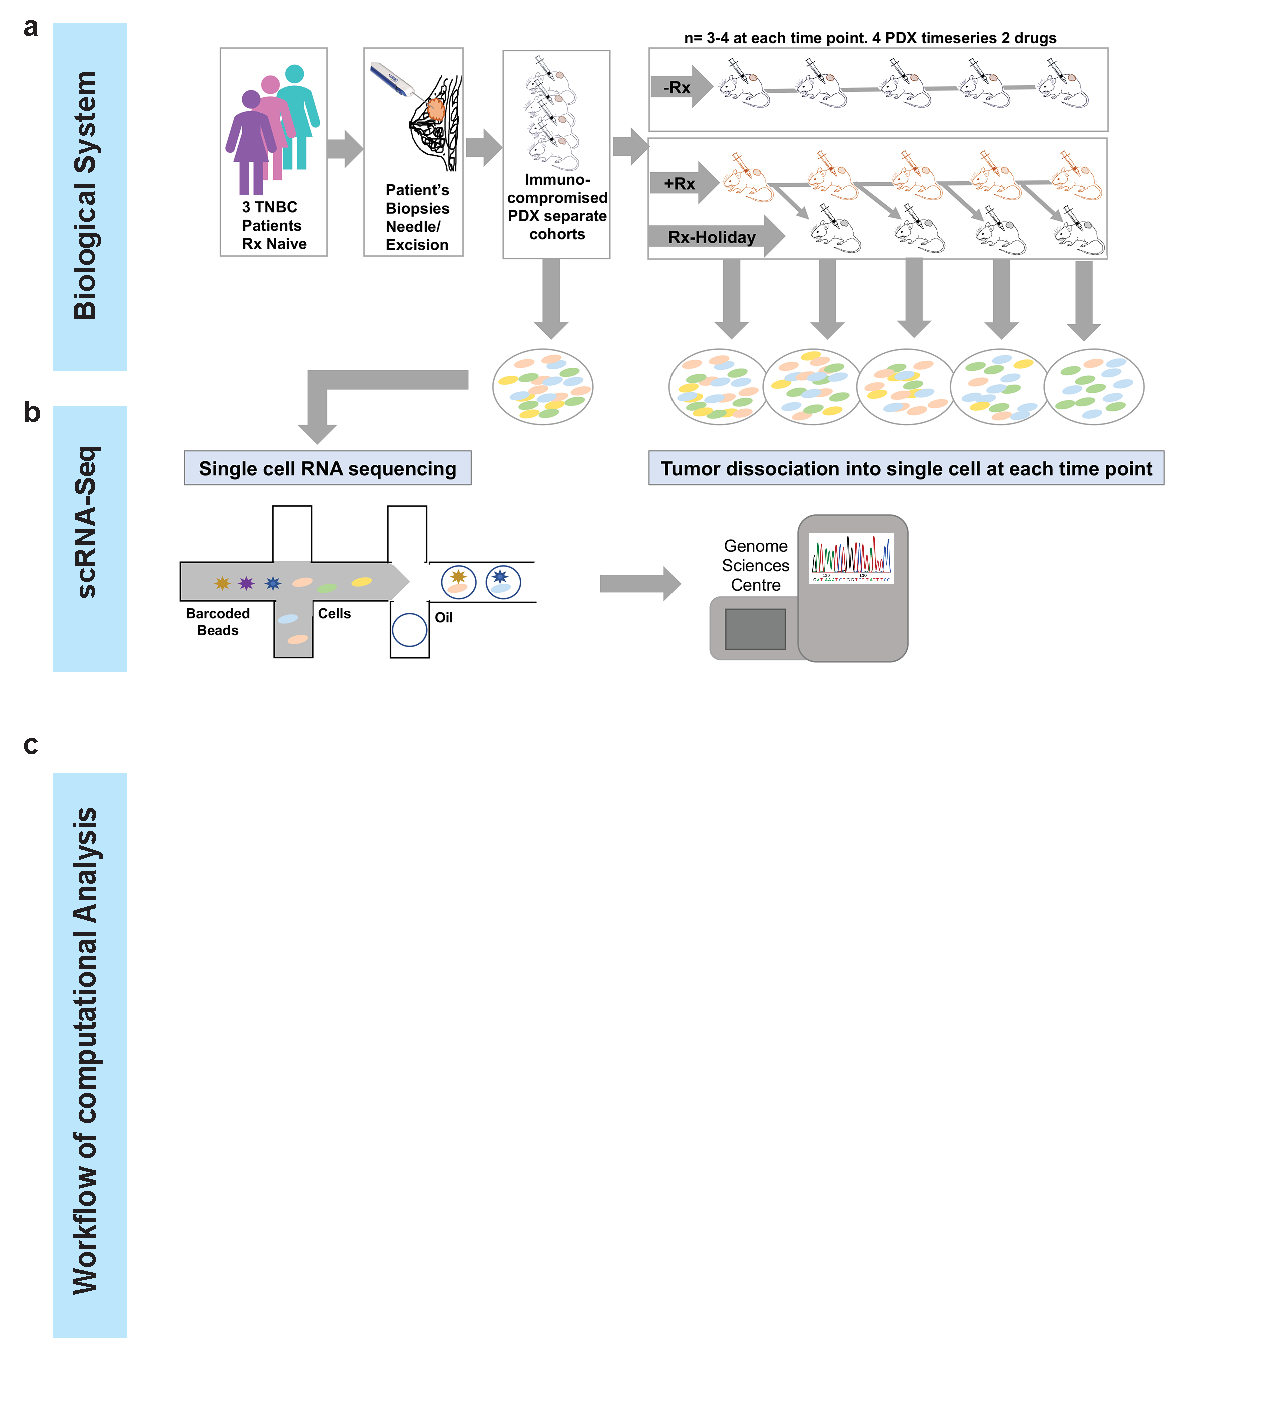
\includegraphics[width=\textwidth]{Figures/fig1schematicsoverview.pdf}
	
\caption[Schematic overview of experimental design and analysis pipeline.]
	{\small
	\textbf{Need to update: Schematic overview of experimental design and analysis pipeline.}
	   Upper panel shows biological systems used to acquire single cell RNA sequencing data. The time point tumors are similar to DLP+ samples in Chapter 4. After applying filters and normalization, various packages are used for analysis as mentioned in the lower half of the schematics.
	 
	}
	\label{fig:fig1schematicsoverview}
\end{figure}


Un-like genomic clones that could get selected in resistant phenotype \cite{salehi2020single}, we still are not clear whether the cell-states are acquainted for this kind of behaviour or the selected states are pre-existing in the cancer population and under continues pressure shows obvious dynamics or there is a transition from one state to another that ultimately gets selected over time. Because of difficulty to analyse longitudinal patient's samples for single cell gene expression and lack of multiple longitudinal pre-clinical breast cancer models, these questions remains unexplored. Here we set to examine three breast cancer patient derived xenografts (PDX) that were serially challenged for around 4-5 cycles with the drug until they started showing less response to the treatment. We wanted to understand the magnitude of fluctuations in gene expression from sensitive to resistant phenotype.


 \section{Synopsis}
   From the previous chapter we know that the population changes with the tumor growth from one passage to another with and without the drugs. We see the shifts in the clones and some clones get selected and others disappear.
   Now in this chapter, first of all we sought to determine whether under neutral conditions when there is no drug pressure what proportion of the transcriptomes might be copy number driven just due to the natural evolution of the copy number clones. This allows us to understand the stability of the gene expression in our timeseries models in the absence of drugs.
   Next, we explored that on drug being introduced into the system, how much of the drug induced change in expression is dependent on the copy number and which are independent.




\section{Results}


\subsection{Clone-specific genotypes underpin clone-specific gene expression programs}
We profiled the impact of clone specific gene expression changes as a higher order representation of phenotypic properties. We tested if the genotypes of high fitness clones exhibited changes in their transcriptional program, with scRNAseq performed on matched aliquots of samples sequenced using DLP+ on the serially passaged triple-negative breast cancer patient-derived xenografts from Chapter 4 as substrates \textbf{(\autoref{fig:treatedtimeseriesmanuscript)}}.

\subsubsection{Copy number change and scRNAseq expression revealed legitimate correlation across PDX timeseries}
  In our approach, we assume clones are defined through grouped cell subsets which share to a first approximation similar genomic copy number structure (e.g., through phylogenetic reconstruction or dimensionality reduction) \cite{laks2019clonal}. Based on this relationship we applied
  \texttt{clonealign} approach \cite{campbell2019clonealign} to reveal clone-specific phenotypic properties across all samples.
  Each point is taken as the proportion of DLP cells in a clone horizontal axis versus the proportion of the scRNAseq cells in the same clone. The  correlation for all clones were then calculated by using Pearson correlation coefficient formula. The heat maps of SA609 TNBC PDX \textbf{(\autoref{fig:UnRxseries} h)} and SA535 TNBC PDX \textbf{(\autoref{fig:SA535analysis} a,e)} exhibit more complex heterogeneity at copy number space along with structural genomic rearrangements as compared to SA1035 TNBC PDX \textbf{(\autoref{fig:SA1035Rxnew} a, e)}. Our results showed DLP+ and \texttt{clonealign} clone abundance measures were positively correlated across all libraries \textbf{\autoref{fig:fig2_clonealignembeddings.pdf} a, d, g}. Importantly, SA535 TNBC treated with cisplatin present the high confidence correlation with Pearson correlation 0.97 (p$<$0.001), followed by its CX-5461 treated series, presenting Pearson correlation of 0.94 (p$<$0.001) \textbf{\autoref{fig:fig2_clonealignembeddings.pdf} g}. However, SA609 PDX timeseries samples present a Pearson correlation coefficient of 0.94 (p$<$0.001) \textbf{(\autoref{fig:fig2_clonealignembeddings.pdf} a)} and SA1035 PDX with Pearson correlation of 0.78 (p$<$0.001) \textbf{(\autoref{fig:fig2_clonealignembeddings.pdf} d)}.
  
  

\begin{figure}
\centering
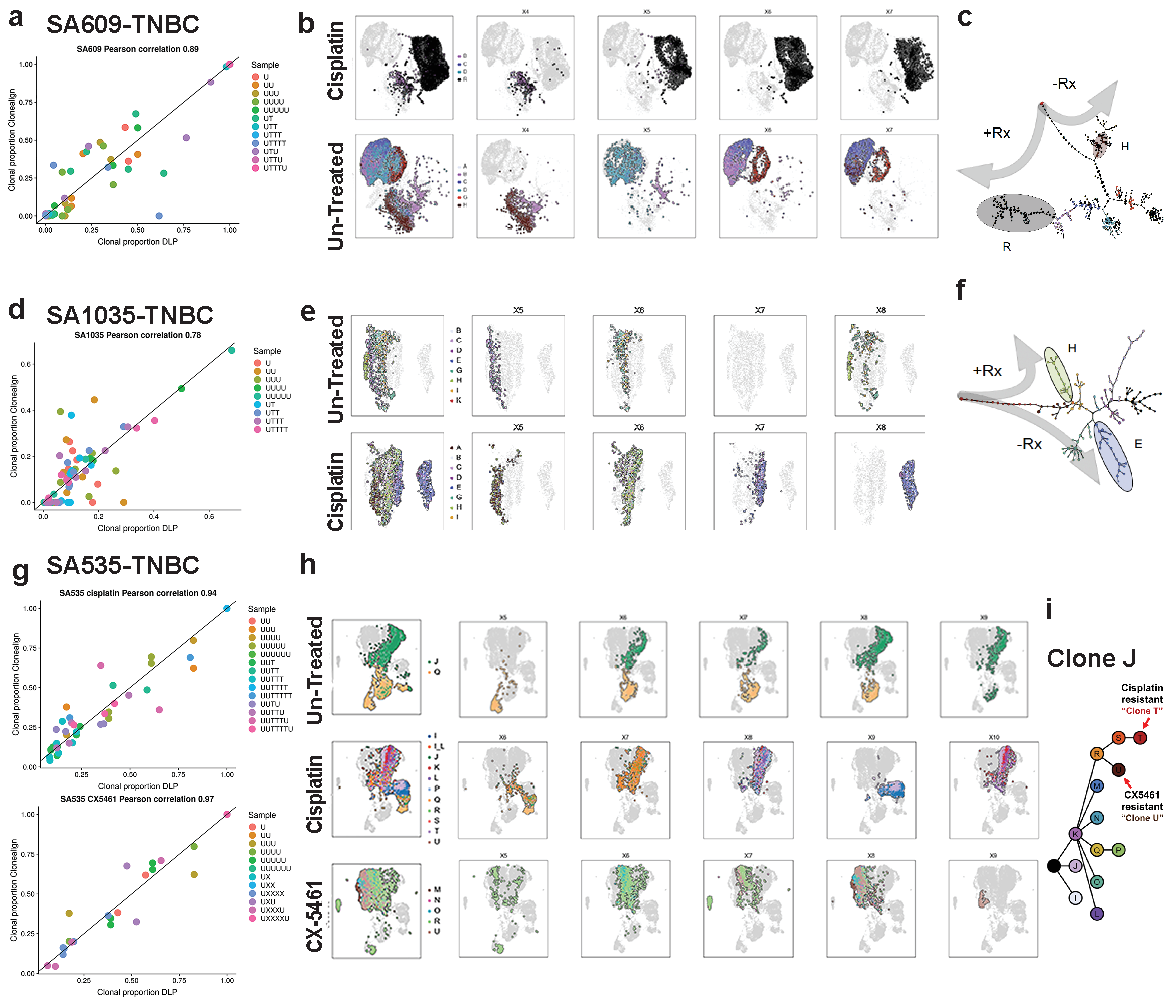
\includegraphics[width=\textwidth]{Figures/fig2_clonealignembeddings.pdf}
	
\caption[Gene expression impacts of clone-specific copy number profiles]
	{\small
	\textbf{Gene expression impacts of clone-specific copy number profiles.}
	   \textbf{(a)} \texttt{clonealign} clonal proportions vs DLP+ clonal proportions of SA609 PDX timeseries samples indicating positive correlation (Pearson correlation from 0.89).
	    \textbf{(b)} Low dimensional \ac{UMAP} embeddings of matching scRNAseq libraries across the SA609 TNBC timeseries. Left top and bottom panels show treated and untreated complete embedding annotated with clonealign assignments and right all panels show the density of cell clusters over the timeseries X4-X7.
	     \textbf{(c)} Phylogeny of SA609 taken from previous chapter to recall emerged clones with or without drug. 
	     \textbf{(d)} Same like \textbf{(a)} but for SA1035 PDX and Pearson correlation is 0.78. \textbf{(e)} Same like \textbf{(b)} but for SA1035 starting from X5-X8. \textbf{(f)} Same like \textbf{c} but for SA1035. \textbf{(g)} Same like \textbf{a} but for SA535 PDX and Pearson correlation is 0.94 for cisplatin treated and 0.97 with CX-5461 treated. \textbf{(h)} Same like \textbf{b} but for SA535 starting from X5-X9, X10.
	}
	\label{fig:fig2_clonealignembeddings.pdf}
\end{figure}



\subsubsection{Single cell RNAseq clusters exhibit a dynamic pattern of global expression over time which tracked with clone assignments}
Next, we visualized the data using UMAP \cite{becht2019dimensionality}, dimensionality reduction method, to aggregate cells into treated and untreated subpopulations while retaining the relationship between subpopulations. scRNAseq embeddings displayed a dynamic pattern of global expression over time with and without treatment, which tracked with clone assignments indicating co-variation of transcriptional properties with clonal abundance \textbf{\autoref{fig:fig2_clonealignembeddings.pdf}}. UMAP Visualization of clusters identified clone H clusters in untreated setting and clone R clusters, in the cisplatin treated series of SA609 TNBC PDX, purified over time matching their genomically defined counterparts \textbf{(\autoref{fig:fig2_clonealignembeddings.pdf} b)}. Similarly, clone E in untreated and clone H in treated timeseries of SA1035  \textbf{(\autoref{fig:fig2_clonealignembeddings.pdf} e)}, clustered uniquely at the later time points. \textbf{\autoref{fig:fig2_clonealignembeddings.pdf} c, f} reminding the clones emerging with and without treatment through the phylogeny of DLP+ from chapter 4, in SA609 and SA1035, respectively.  SA535 TNBC PDX all three arms of untreated, treated with cisplatin and CX-5461, exhibited aggregation of similar patterns of clusters that favours emerging of genomic clones in their respective series. Clone J, in untreated control timeseries \textbf{(\autoref{fig:fig2_clonealignembeddings.pdf} h, upper panel)}, clone T, in cisplatin timeseries 


\subsection{Copy number dependent in-cis and trans regulated gene expression rates in scRNAseq data set}



\begin{figure}
\centering
  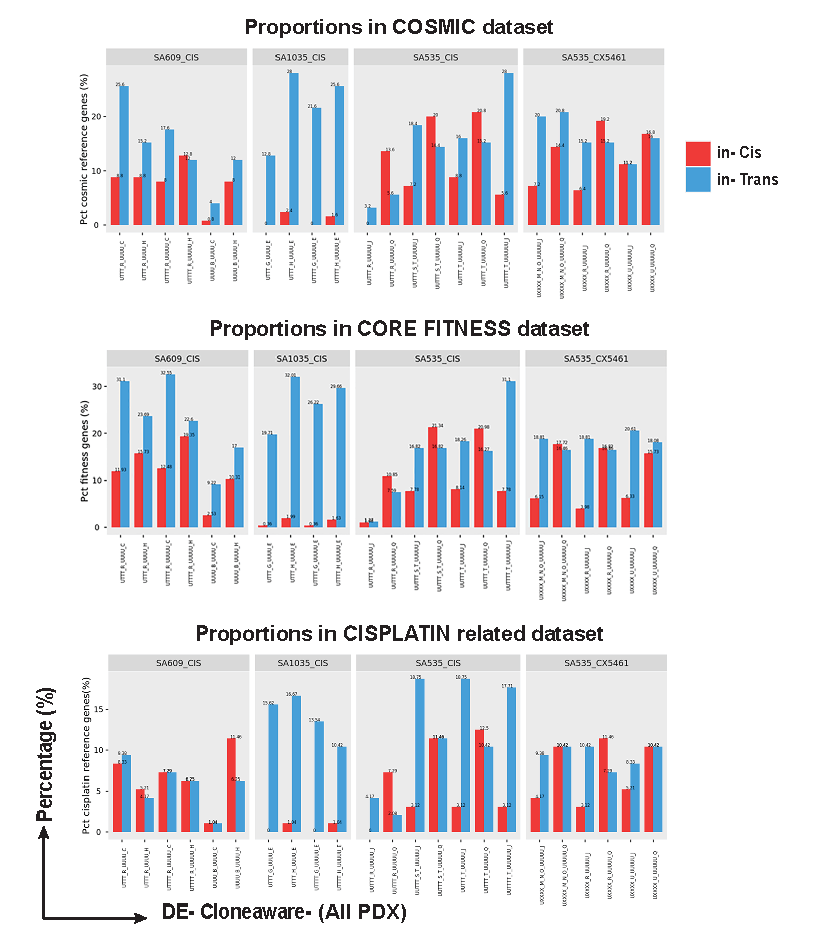
\includegraphics[width=\textwidth]{Figures/fig3_In_cispercentage.pdf}
	
\caption[Proportion of in-cis and in-trans regulated gene expression in scRNAseq data]
	{\small
	\textbf{Proportion of cis and trans regulated gene expression in scRNAseq data.}
	   Horizontal axis shows differential expression between two selected clones from all the three PDX treated and un-treated timeseries. Vertical axis gives percentage presence of genes in-cis or in trans. red bars represent in-cis and blue bars represent in -trans regulated gene expression.
	   \textbf{(Upper)} This graph gives us percentage of genes by looking into the gene data set from COSMIC cancer gene dataset \cite{vogelstein2013cancer} that corresponds to our clone aware \ac{DE}.
	    \textbf{(Middle)} same like upper plot but looking into CORE FITNESS data set \cite{behan2019prioritization}.
	     \textbf{(Lower)} Same like above but looking into cisplatin related gene list curated from literature.
	    
	}
	\label{fig:fig3_In_cispercentage}
\end{figure}



\subsection{Differential expression  analysis of resistant and sensitive clones}




\begin{figure}
\centering
  \includegraphics[width=\textwidth]{Figures/fig4_Volcanotrackplots2.pdf}
\caption[DE of resistant and sensitive clonealign defined clones]
	{\small
	\textbf{Differential expression of resistant and sensitive clones.}
	\textbf{(a)} Volcano plot from SA609 -log10(FDR) plotted against log2 fold change of pairwise differential gene expression between resistant and sensitive clones. Manhattan plot (genome-wide view) of differential gene expression between pairs of clones, R vs H corresponding to change in gene expression (Right).
	    \textbf{(b)} Same like \textbf{a} but in SA1035 and comparing between pairs of clones, H vs E. 
	     \textbf{(c)} Same like \textbf{a} but in SA535 (cisplatin) and comparing between pairs of clones, S\_T vs J. 
	     \textbf{(d)} Same like \textbf{a} but in SA535 (CX-5461) and comparing between pairs of clones, U vs J.
	   \textbf{(e)} Barplot showing copy number driven percentage of in cis or in trans up and down regulation of genes.
	   \textbf{(f)} Barplots showing summary of total in cis and in trans proportion in the whole data set.
	     \textbf{(g-j)} Manhattan plot (genome-wide view) of differential gene expression between pairs of clones, from \textbf{a, b, c, d}. }
	\label{fig:fig4_Volcanotrackplots2}
\end{figure}




\begin{figure}
\centering
  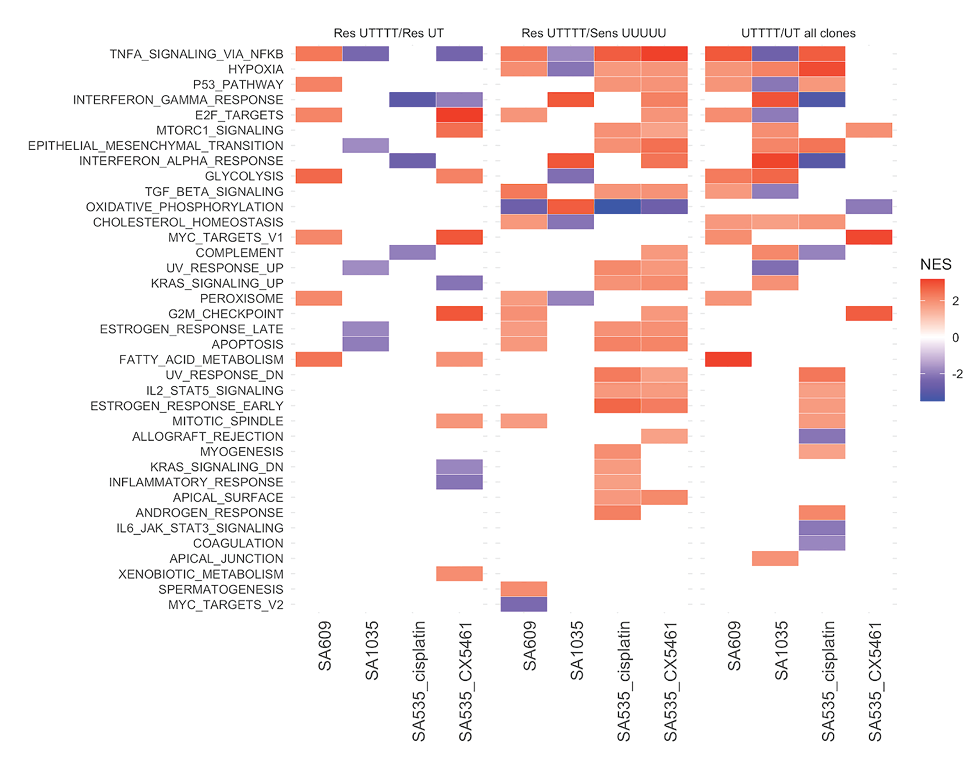
\includegraphics[width=\textwidth]{Figures/fig5pathwaysnetwork.pdf}
\caption[Pathways enrichment analysis of PDX timeseries]
	{\small
	\textbf{Pathways enrichment analysis of PDX timeseries.}
	 Vertical axis on the left enlisting the pathways involved under various conditions in timeseries PDXs. Left panel comparing resistant clone versus clone exposed to only one cycle of drug. Middle panel comparing resistant versus sensitive clone in all PDXs. Right panel comparing last treated timepoint as a whole with first treated timepoint. Horizontal axis is showing the names of PDXs.
	}
	\label{fig:fig5pathwaysnetwork}
\end{figure}

\begin{figure}
\centering
  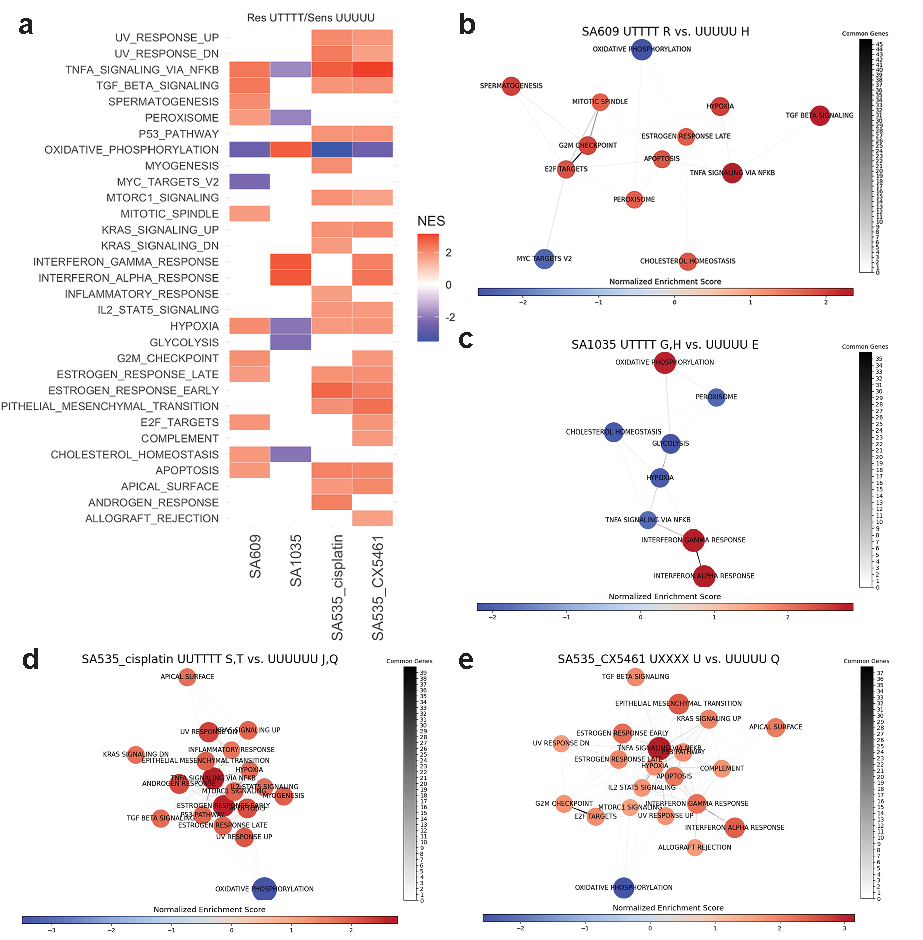
\includegraphics[width=\textwidth]{Figures/fig6resistantsensitivenetwork.pdf}
\caption[DE of resistant and sensitive clonealign defined clones]
	{\small
	\textbf{Pathway enrichment network comparing resistant and sensitive clones across timeseries PDX.}
	\textbf{(a)} Normalized enrichment score of Pathways between resistant and sensitive clone of all treated timeseries PDXs.
	    \textbf{(b)} Pathway enrichment network comparison of clone R vs clone H in SA609. Colour of grey to black lines between the pathways show strength of common genes on scale vertically drawn on right side. 
	     \textbf{(c)} Same like \textbf{a} but in SA1035  and comparing pathways between pairs of clones, G\_H vs E. 
	     \textbf{(d)} Same like \textbf{a} but in SA535 (Cisplatin) and comparing between pairs of clones, S\_T vs J\_Q.
	 \textbf{(e)} Same like \textbf{a} but in SA535 (CX-5461) and comparing between pairs of clones, U vs Q.}
	
	\label{fig:fig6resistantsensitivenetwork}
\end{figure}










\subsubsection{SA609-TNBC-FBI PDX up regulated pathways in resistant clone}


\subsubsection{SA535-TNBC-BRCA deficient PDX up regulated pathways in resistant clone}
Next we compared the emerging clone under drug pressure with the clone that could not survive the repeated drug exposures. We identified the following significantly up regulated pathways:
- Apoptosis, Epithelial mesenchymal transition, Hypoxia, mitotic spindle, MTORC1 signaling, MYC targets-V1, P53 pathway, TGF Beta signaling, TNFA signalling via NFKB, UV response up, UV response down, KRAS signaling, Angiogenesis, PI3K AKT MTOR signaling, unfolded protein response.


\subsubsection{SA1035-TNBC-APOBEC deficient PDX up regulated pathways in resistant clone}




\subsection{key Pathways and genes shared among the three TNBC PDX}




\subsection{Distinct genes monotonically increasing and decreasing with drug} 




{\chapter{Conclusions and discussion}

}
\label{ch:Chapter6}

\section{Major findings}
Predicting the dynamics of malignant cells in cancers and deconstructing the molecular basis of resistance and metastasis can be achieved by repeated observation of cell populations with shared genotypes and phenotypes. In this thesis project we have applied this concept to show that cell population dynamics in cancer can be resolved by assigning cells to specific clones, defined by copy number. We repeatedly observe the similar fitness coefficients for the same copy number genotypes, showing deterministic behaviour. The fitness differences between most clones is small, despite large changes in clone prevalence over time.


\subsection{Identification and confirmation of a significant transcriptomic signature under various conditions}

In chapter 3, we set out to assess the impacts of tissue dissociation and data analysis quality control, taking advantage of a recently described protease active at low temperatures (on ice), to contrast the effects of low temperature protease solid tissue dissociation with those of more routinely used collagenase at 37\textdegree C. Identification and confirmation of a significant transcriptomic signature comprising 512 core genes in response to collagenase tissue digestion at 37\textdegree C. Significantly, this signature is highly confounded with known cancer biology, comprising a large number of tumour stress and resistance markers. We demonstrate for the first time that this signature can be mitigated by tissue digestion with a cold protease (active at 6\textdegree C) derived from a Himalayan glacier resident bacterial species.

Predominantly, we FACS sorted lymphoblastoid cells into live, dying, and dead populations (with/without induction of cell death with TNF-alpha) to characterize the efficacy of standard scRNA-seq QC practices on removing dead and dying cells. In doing so, we identify a subset of dead cells which would not be filtered by standard practices. We reported that cells that were FACS sorted as either live, dying, or dead (with/without induction of cell death with TNF-alpha), were present in all three clusters, emphasizing that the although the transcriptomic state and and the surface marker of the cell are correlated but they are not the same. Such concepts are implicative  of ``pseudotime'' in single-cell trajectory analysis, whereby developmentally ordering cells transcriptomically can lead to early or late cells being placed at variable positions along the pseudotime trajectory \cite{campbell2018descriptive, campbell2018uncovering}. 
 Furthermore, we identified a subpopulation of cells (enriched for dying and dead) that showed increased expression of MHC Class I genes, indicative of stress and which may distinguish these cells from otherwise transcriptomically healthy cells. This finding could be pertinent to the studies of immune response in cancer.
 

 Finally, we identified a conserved collagenase-associated transcriptional pattern including induction of stress and heat shock genes, consistent with a transcriptional response identified in a subset of muscle stem cells \cite{van2017single}, and which was minimized when samples were dissociated at cold temperatures with a cold active serine protease. We demonstrate that both digestion time and collagenase contribute to the transcriptomic stress response in single cancer cells. Therefore, the short incubation time necessary for cold protease as well as the relatively stable transcriptome captured by dissociation at cold temperatures suggests this is a potential alternative to collagenase dissociation for scRNA-seq experiments with tumor tissues. We suggest that each tissue and dissociation method should be assessed for dissociation-induced signatures before undertaking large-scale scRNA-seq experiments. 
 
 Transcription of the identified gene set in chapter 3 as a result of sample preparation methods may mask their induction due to other means. For example, \textit{JUN} and \textit{FOS} are associated with cancer drug resistance and metastatic progression \cite{insua2018stress,fan2017ap, ramsdale2015transcription}. Moreover, though less stark as the core collagenase-associated gene set, cell type-specific effects were observed during dissociation and included increased hedgehog and apical surface pathways in breast epithelial cells and reactive oxygen species pathways in cytotoxic T cells and myofibroblasts. Taken together, these findings indicate that all cell types exhibit some level of stress response to dissociation with collagenase, with some cell types exhibiting cell type-specific responses. These stress responses, which may significantly influence the interpretation of scRNA-seq data, are minimized by dissociation at cold temperatures.
 

\subsection{Copy number could be associated with clonal fitness in \textit{Tp53} mutant human breast cancers}
From chapter 4, clonal expansions were observed in \textit{TP53} mutant human breast cancer cells, through serial passaging, single cell sequencing and fitness modeling of four patient derived xenografts. Bulk WGS and DLP+ confirmed all four tumors were p53 mutant (SA609: p.R213X; SA1035: p.C242F; SA532: p.A159P; SA535: frameshift chr17:7578490, \textbf{\autoref{tab:Tp53mutationofPDX}} with bi-allelic and truncal distribution across clones.
We first studied clonal evolution in untreated PDX models, sampled over 927 days for HER2+ SA532, 619 days for TNBC-SA609, 381 days for TNBC-SA1035 and 353 days for TNBC-SA535. DLP+ were generated and sequenced, yielding a median of 1,116 single cell genomes per sample (95,275 total cells). 

All series exhibited progressively higher tumour growth rates over time. In contrast to HER2+SA532, all TNBC PDX models exhibited evidence of clonal diversification associated with copy number alterations and selective coefficients consistent with positive selection over time \textbf{\autoref{fig:landscapefitness}}. 
For TNBC-SA609, Clones E  (1+s= 1.07 $\pm$ 0.02) and H (1+s=1.02 $\pm$ 0.02) had the highest selective coefficients and exhibited growth from undetectable levels to 59 and 32\% respectively by timepoint X10.
In SA535 TNBC, three major clones were observed with clone G characterized by loss of chromosome X exhibiting a clonal expansion from minor prevalence as passage X5 to near dominance at 76\% at passage X9. Similar patterns were observed for the other TNBC cases.  
For TNBC-SA1035, 11 clones were detected with clone E expanding to 69\% at passage X8 from minor prevalence at the initial timepoint. The predicted selective coefficient of clone E was(1+s = 1.06 $\pm$ 0.03) . By contrast, Clones A and K had initial prevalences of 20 and 9\% ,respectively, but were not detectable by the last timepoint. 

Having established quantification of CNA associated subclone fitness, we next asked how clone-specific fitness is influenced under drug treatment. We tested how cisplatin, a standard therapy for primary TNBC, impacted the stability of the fitness landscape of the three independent PDX TNBC series (TNBC-SA609, TNBC-SA535, TNBC-SA1035).

For TNBC-SA609, we implemented a more extensive experimental design to account for potential differences in transplantation from fresh tissues relative to those subjected to a freeze-thaw cycle used in serial propagation between X3 and X4. Three treated lines and Line 2 untreated samples were propagated from an X3 frozen sample, whereas Line 1 untreated samples were propagated from dissociation of a fresh specimen. Technical replicates were also collected for Line 1 and 2.    

In each series, we observed an inversion of the clone fitness landscape \textbf{\autoref{fig:landscapefitness}}, left and right panels), resulting in suppression of clones that dominated in the absence of treatment and emergence of low fitness and/or previously unobserved CNA genotypes. For example, in the treatment branch of TNBC-SA609 Line 2, the growth dynamics over (X3 U; X4 UT; X5 UTT; X6 UTTT; X7 UTTTT) and \textit{fitClone} modeling revealed that resistant clones (A, R)- constituting a branch of the phylogeny derived from clone B,  monotonically increased on treatment. A technical replicate of X7 in Line 2 showed a similar composition and nearly all cells consisted of Clones B and R.  In Line 1, a sibling clone of A, clone R reproducibly swept to fixation on treatment. Notably, after the first treatment cycle, all three lines showed expansion of clone B and its derivative R at timepoint X4 and a contraction of clone H.



\begin{figure}
\centering
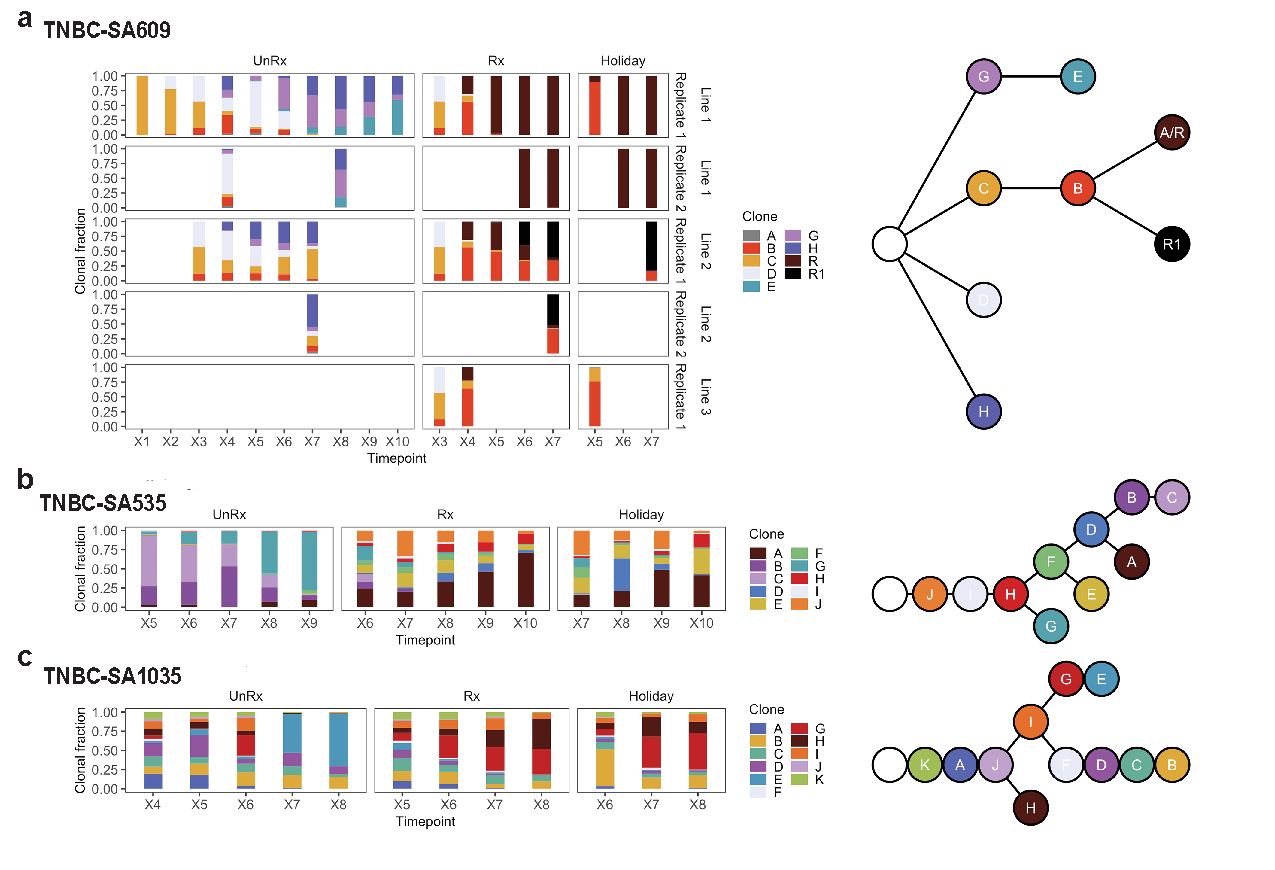
\includegraphics[width=\textwidth]{Figures/All3barplots.pdf}
\caption[Summary of number of genes \textit{in-cis} and \textit{in-trans}]
	{\small
	\textbf{}
	Observed clonal abundances in TNBC-SA609, TNBC-SA535-Rx and TNBC-SA1035-Rx, for each tumor sampled for scWGS. Right vertical axis represents the line. Right panels show clonal phylogenies.
}
    \label{fig:All3barplots}
    \end{figure}

Notably, the high fitness clones H, G, D from the untreated series exhibited low fitness coefficients in the treatment series and were no longer detected \textbf{\autoref{fig:landscapefitness}}. This was evident in the relative fitness ranking \textbf{\autoref{fig:landscapefitness} d}, clone bipartite fitness rank) and absolute fitness values (reffig{fig:landscape} d, probability of positive selection). Conversely, Clones A, B,  and C, comprising a low fitness phylogenetic superclade, distinct from high fitness clone H in the untreated series, were the precursors to the resistant clone R \textbf{\autoref{fig:landscapefitness}}, \textbf{\autoref{fig:All3barplots}}. 

In the TNBC-SA535 and TNBC-SA1035 treatment series, similar patterns of low fitness clones in the untreated series expanding on treatment (clone A, in TNBC-SA535; clones G, H, in TNBC-SA1035), with the fittest clones under no treatment (e.g. TNBC-SA535 clone G; TNBC-SA1035 clone E) decreasing to near zero prevalence. The majority of the other clones were also impacted by treatment in all three series. For example, in SA535, the relative fitness rank of Clone G fell from first to sixth and clone B fell from third to tenth.  Clone H increased from sixth to second and Clone J from seventh to third.  

In SA1035, Clone E fell from first to seventh and clone A fell from third to eighth. Clone G increased from tenth to second.  The impact across the whole fitness landscape was reflected in the probability of positive selection distributions.  These distributions were statistically significantly increased in the treatment series  (\textbf{\autoref{fig:landscapefitness}} d), indicating that fewer clones were under neutral selection as a function of cisplatin, and that the fitness landscape exhibited a wider variance between clones.

For example, in the treatment branch of TNBC-SA609 replicate treated, Line 2, the growth dynamics over (X3 U; X4 UT; X5 UTT; X6 UTTT; X7 UTTTT) and \texttt{fitClone} modeling revealed that a new ``Clone R1'', constituting a branch of the phylogeny derived from clone B, monotonically increased on treatment.  A technical replicate of X7 in Line 2 showed a similar composition, nearly all cells consisted of Clones B and R1.  In Line 1 a sibling clone of R1, clone R reproducibly swept to fixation on treatment.  Notably, after the first treatment cycle, all three lines showed expansion of clone B and its derivative R at timepoint X4 and a contraction of clone H.

Moreover, the heat maps of TNBC-SA609 and TNBC-SA535 PDX \textbf{(\autoref{fig:mediangenotypes}}) exhibited more complex heterogeneity at copy number space along with structural genomic rearrangements as compared to TNBC-SA1035 PDX.


\subsection{Clone specific genotypes drives clone-specific gene expression programs}

After establishing the fitness of genomic clones in the presence or absence of chemotherapies in chapter 4, we next sought to uncover the basis of how copy number variation alters gene expression in complex cell mixtures. In parallel, we sequenced single-cell RNA from independent cell populations and mapped for genome-transcriptome association. 
We revealed that gene expression states can be assigned to cancer clones using single-cell RNA and DNA sequencing independently sampled from a heterogeneous cell populations. We also demonstrated that single cell RNAseq clusters exhibited comparably monomorphic pattern of global expression over time which could be tracked with clonal assignments.

%----------------------------------------------------------

 \begin{table}[htbp]
   \centering
   \caption{Number of genes in DE* of resistant versus sensitive clones and their regulation status in all TNBC PDX series}
     \begin{tabular}{|l|l|l|}
     \hline
     \multicolumn{1}{|l|}{\textbf{No. of genes**}} & \multicolumn{1}{|l|}{\textbf{Percent genes (\%)}} & \textbf{Gene regulation} \\
     \hline
     \multicolumn{1}{|l|}{\textbf{SA609-TNBC}} &   &  \\
     438 & 12.9 & In\_cis\_Decrease\_DownRegulated \\
     76 & 2.2 & In\_cis\_Decrease\_UpRegulated \\
     214 & 6.3 & In\_cis\_Increase\_DownRegulated \\
     926 & 27.3 & In\_cis\_Increase\_UpRegulated \\
     966 & 28.4 & In\_trans\_DownRegulated \\
     778 & 22.9 & In\_trans\_UpRegulated \\
     \multicolumn{1}{|l|}{\textbf{SA1035-TNBC}} &   &  \\
     93 & 2.6 & In\_cis\_Decrease\_DownRegulated \\
     18 & 0.5 & In\_cis\_Decrease\_UpRegulated \\
     19 & 0.5 & In\_cis\_Increase\_DownRegulated \\
     116 & 3.3 & In\_cis\_Increase\_UpRegulated \\
     1661 & 47.2 & In\_trans\_DownRegulated \\
     1612 & 45.8 & In\_trans\_UpRegulated \\
     \multicolumn{1}{|l|}{\textbf{SA535-TNBC-cisplatin}} &   &  \\
     473 & 9.8 & In\_cis\_Decrease\_DownRegulated \\
     271 & 5.6 & In\_cis\_Decrease\_UpRegulated \\
     43 & 0.9 & In\_cis\_Increase\_DownRegulated \\
     253 & 5.2 & In\_cis\_Increase\_UpRegulated \\
     1068 & 22.1 & In\_trans\_DownRegulated \\
     2716 & 56.3 & In\_trans\_UpRegulated \\
     \multicolumn{1}{|l|}{\textbf{SA535-TNBC-CX-5461}} &   &  \\
     697 & 21.5 & In\_cis\_Decrease\_DownRegulated \\
     91 & 2.8 & In\_cis\_Decrease\_UpRegulated \\
     45 & 1.4 & In\_cis\_Increase\_DownRegulated \\
     345 & 10.6 & In\_cis\_Increase\_UpRegulated \\
     924 & 28.5 & In\_trans\_DownRegulated \\
     1145 & 35.3 & In\_trans\_UpRegulated \\
     \hline
     \end{tabular}%
     
   \label{tab:NumberofDEgenesandstatus}%
   
   \small\textbf{(*Differential expression, ** (FDR$<$0.01, p$<$0.05))}.
 \end{table}%

%----------------------------------------------------------

Importantly, we were able to dissect the regulation status of  differentially expressed genes between genomically defined resistant and sensitive clones in all TNBC PDX series. For example, pairwise comparisons of clone-specific differential gene expression in \textbf{SA609} , between resistant clone R and sensitive clone H (FDR$<$0.01, p$<$0.05), identified 926 genes having clone specific copy number increase in expression \textit{(incis\_IU)}, whereas, 438 genes were downregulated with decrease in copy number \textit{(incis\_DD)}. Whereas, 966 genes were downregulated and 778 were upregulated  independent of change in copy number \textit{in trans} \textbf{(\autoref{fig:Volcanotrackplots2.pdf} a, left)}, Summary of all 4 PDX series \textbf{\autoref{tab:NumberofDEgenesandstatus}}. The Manhattan plot confirming the increase and decrease in copy number between clones at that genomic position and its respective change in gene expression \textbf{(\autoref{fig:Volcanotrackplots2.pdf} a, right)}.

In high fitness clones (resistant) with amplifications as distinguishing features, we noted accompanying \textit{in cis} clone-specific differential gene expressions, for example, in SA609-TNBC, \textit{CRABP1} in resistant clone of SA609 TNBC PDX (clone R with copies of Chr15q) and  \textit{TCF4} in clone R with 3 copies of Chr20q). Summary of top 20 clone specific upregulated genes and their change in copy number are in \textbf{Chapter 5}.

Together these data indicate that clonal genotypes driving high fitness trajectories are accompanied by changes in gene expression at both chromosomal and focal level copy number alterations with variable individual gene regulation status.


\section{Limitations and future directions}

IN chapter 3, our novel and single cell RNA seq analysis data provided a comprehensive set of information regarding tissue handling and its effects on sequencing analysis and biological interpretation. Though cell type-specific gene expression effects in response to digestion method were evident, these findings indicate that all cell types exhibit some level of stress response to dissociation with collagenase, with some cell types exhibiting cell type-specific responses. 
However, in large scale drug studies where stress is also induced by chemotherapies and we are interested in studying various relationships of pathways and its downstream effectors, we need to be careful in making choices of digestion enzymes and conditions. 

Another limitation using cold active protease enzyme is that, we didn't compared simultaneously the \ac{DLP+} libraries alongside single cell RNA sequencing at different temperatures. In future, we plan to directly investigate the difference of single cell whole genome sequencing, by comparing digestion at 6\textdegree C and at 37\textdegree C. In addition, while performing our experiments for chapter 3, we noticed that digestion at cold temperature tend to lose more number of cells as compared to digestion at 37\textdegree C. This factor play an important role where we need to make multiple measurements form the same tumor. Moreover, the type of tissue, its consistency and its exposure to either chemotherapy or environmental and genetic perturbations should also be considered as a factor. The choice of digestion enzyme and temperature should be optimized accordingly with before conducting any large scale study.

In chapter 4, we demonstrated a timeseries model of cisplatin resistance in TNBC PDX, which is a standard care and first line of systemic treatment given in most of the cancers. We were intended to explore the underlying clonal dynamics that undergo a change with and without any perturbations to the tumor environment that ultimately lead to tumor resistance. We recognize that establishing causal relationships based on copy number clustering into clones is very difficult and requires more controlled experiments and larger sample sizes. However, exploring the potential correlates of differential fitness may aid in designing follow up experiments. In our timeseries experiments, two out of four PDX series exhibited directional dynamics over either serial passaging or drug intervention. The untreated dynamics were confirmed by two different sets of mixture experiments. In future, more mixture experiments for the timeseries that undergo neutral dynamics over time will explain the tumor biology explicitly. 

Furthermore, in the context of pharmacological intervention, we acknowledge that the drug exposure started from early time points that derives the competition among the clones and infer the fitness of certain clones. It would be very interesting and comparable to conduct experiments where we take later passages of the time series PDXs and start introducing the chemotherapy in the same way. Clonal competitions and fitness in that environment will become obvious.

Pseudobulk, that is merging of single cells to create more sequencing depth for SNV detection is not explained in detail in chapter 4. All the data is being processed and under investigations for SNVs, detailed mutational analysis and integration of allelic imbalance information caused by clone-specific \ac{LOH} events. Follow up replication experiments sequenced at higher depth may be required to rule out the existence of driving mutations. 


In chapter 5, laveraging the newly developed clonealign statistical model,the focus has been on linking transcriptional measurements to genomically defined clones assuming only a copy-number dosage effect on transcript abundance. While the clonealign model allows for integration of allelic imbalance information caused by clone-specific \ac{LOH} events, the sparse expression of germline heterozygous variants detected by the 10X chromium 3' assay demonstrated here makes such information uninformative. However, full-transcript-length single-cell RNA sequencing technologies such as Smart-seq2 \cite{picelli2014full} would allow for further refinement of clonal assignment and represent the appropriate use-case of clonealign’s incorporation of allelic imbalance information.


Furthermore, we explored single cell expression in reference to resistant and sensitive clones defined in the previous chapter. Notable, we indentify many new pathways and genes playing role in our TNBC time series, that are not well studied in context of breast cancer. We have the data of genes that are regulated \textit{in cis} or \textit{in trans}. If there is a loss of copy number that is leading to resistant phenotype, not much could be done, but if the gene is upregulated \textit{in trans}, independent of change in copy number, it could act as a tumor biomarker and gene editing through CRISPRi \cite{larson2013crispr}, for example could be a potential follow up experiment.
Other future experiments would be to use CRISPR/cas9 \cite{doudna2014new} technology for biomarker validations. We have enlisted various combinations of genes, where some are commonly showed up in all treated time series while, some are more specific to certain PDXs. 

Another supporting biological methodology involves epigenetic changes, that may influence the fitness of clones and interrogating the system via orthogonal data types such as chromatin accessibility and/or DNA methylation assays. This is important coupling with single cell RNA expression in context of measuring to gene promoters hypermethylation of tumor suppressor genes  or hypomethylation of oncogenes.








 
 
 
 
 
 
 Single cell RNA seq analysis data can help in a better comprehension of some widespread and more specific biological mechanisms involved in breast cancer progression.that could be further validated pertaining to drug resistance in triple negative through modern techniques, such as, CRISPR/Cas9.

Genetic alterations and the contextual signaling by the microenvironment give rise to an intricate network of pathological mechanisms and molecular pathways


Individual tumors and cancer cells exhibit substantial molecular diversity.

Single cell RNA seq analysis data can help in a better comprehension of some widespread and more specific biological mechanisms involved in breast cancer progression.

% Generally recommended to put each chapter into a separate file
%\include{relatedwork}
%\include{model}
%\include{impl}
%\include{discussion}
%\include{conclusions}

%    3. Notes
%    4. Footnotes

%    5. Bibliography
\begin{singlespace}
\raggedright
\bibliographystyle{abbrvnat}
\bibliography{biblio}
\end{singlespace}

\appendix
%    6. Appendices (including copies of all required UBC Research
%       Ethics Board's Certificates of Approval)
%\include{reb-coa}	% pdfpages is useful here
\chapter{Supporting Materials}

\begin{figure}
\centering
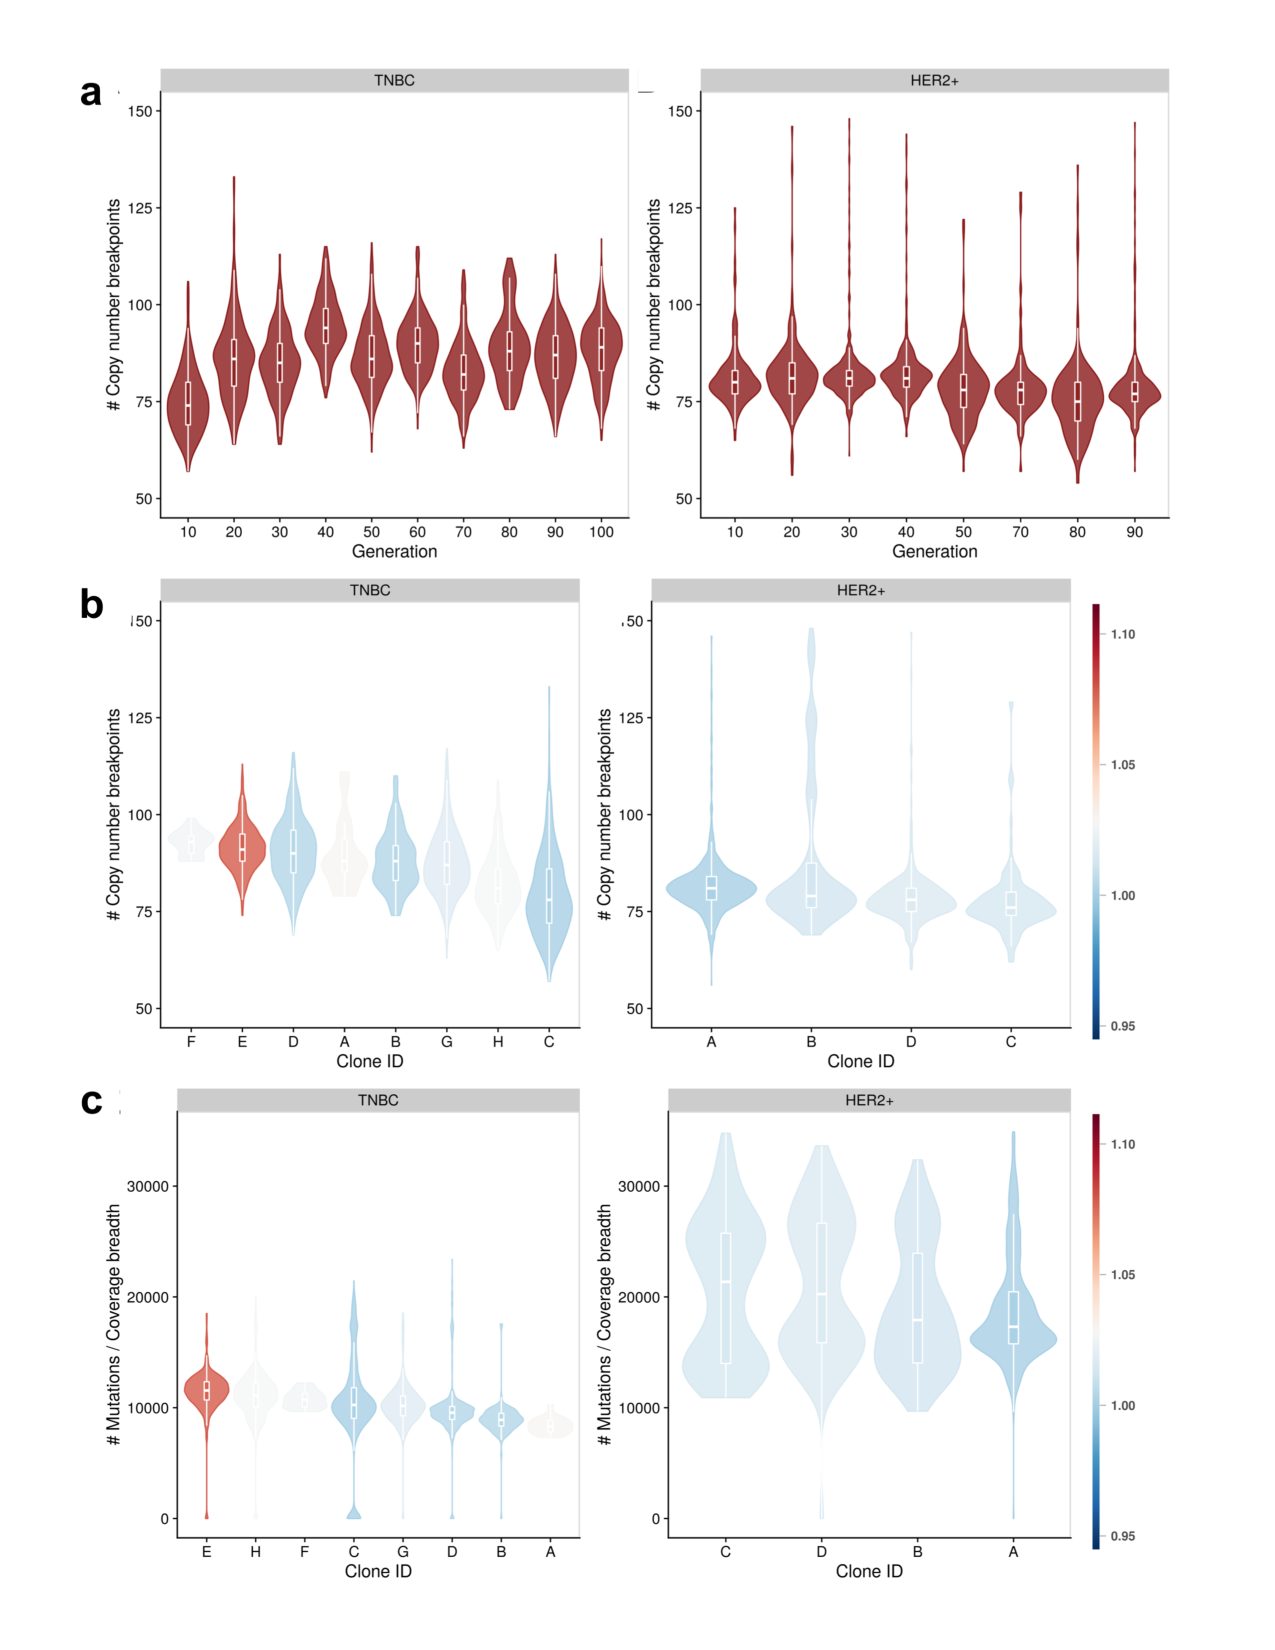
\includegraphics[width=\textwidth]{Figures/chap4/mutationanalysisbreakpoints.pdf}
  \caption[Structural variant and mutation rates of HER2+ and TNBC PDX]
	{\small
	\textbf{Structural variant and mutation rates of HER2+ and TNBC PDX.}
	    \textbf{(a)} Distribution over copy number
breakpoints/cell as a function of generation for left: TNBC, right: HER2+
   \textbf{(b)} Clone specific distributions over copy number breakpoints/cell, coloured by fitness coefficients for left: TNBC, right: HER2+
    \textbf{(c)} Clone specific distributions over point mutations/cell, coloured by fitness coefficients for left:TNBC, right:HER2+
}
    \label{fig:mutationanalysisbreakpoints}
    \end{figure}
%--------------------------------------------------------------------

\begin{figure}
\centering
  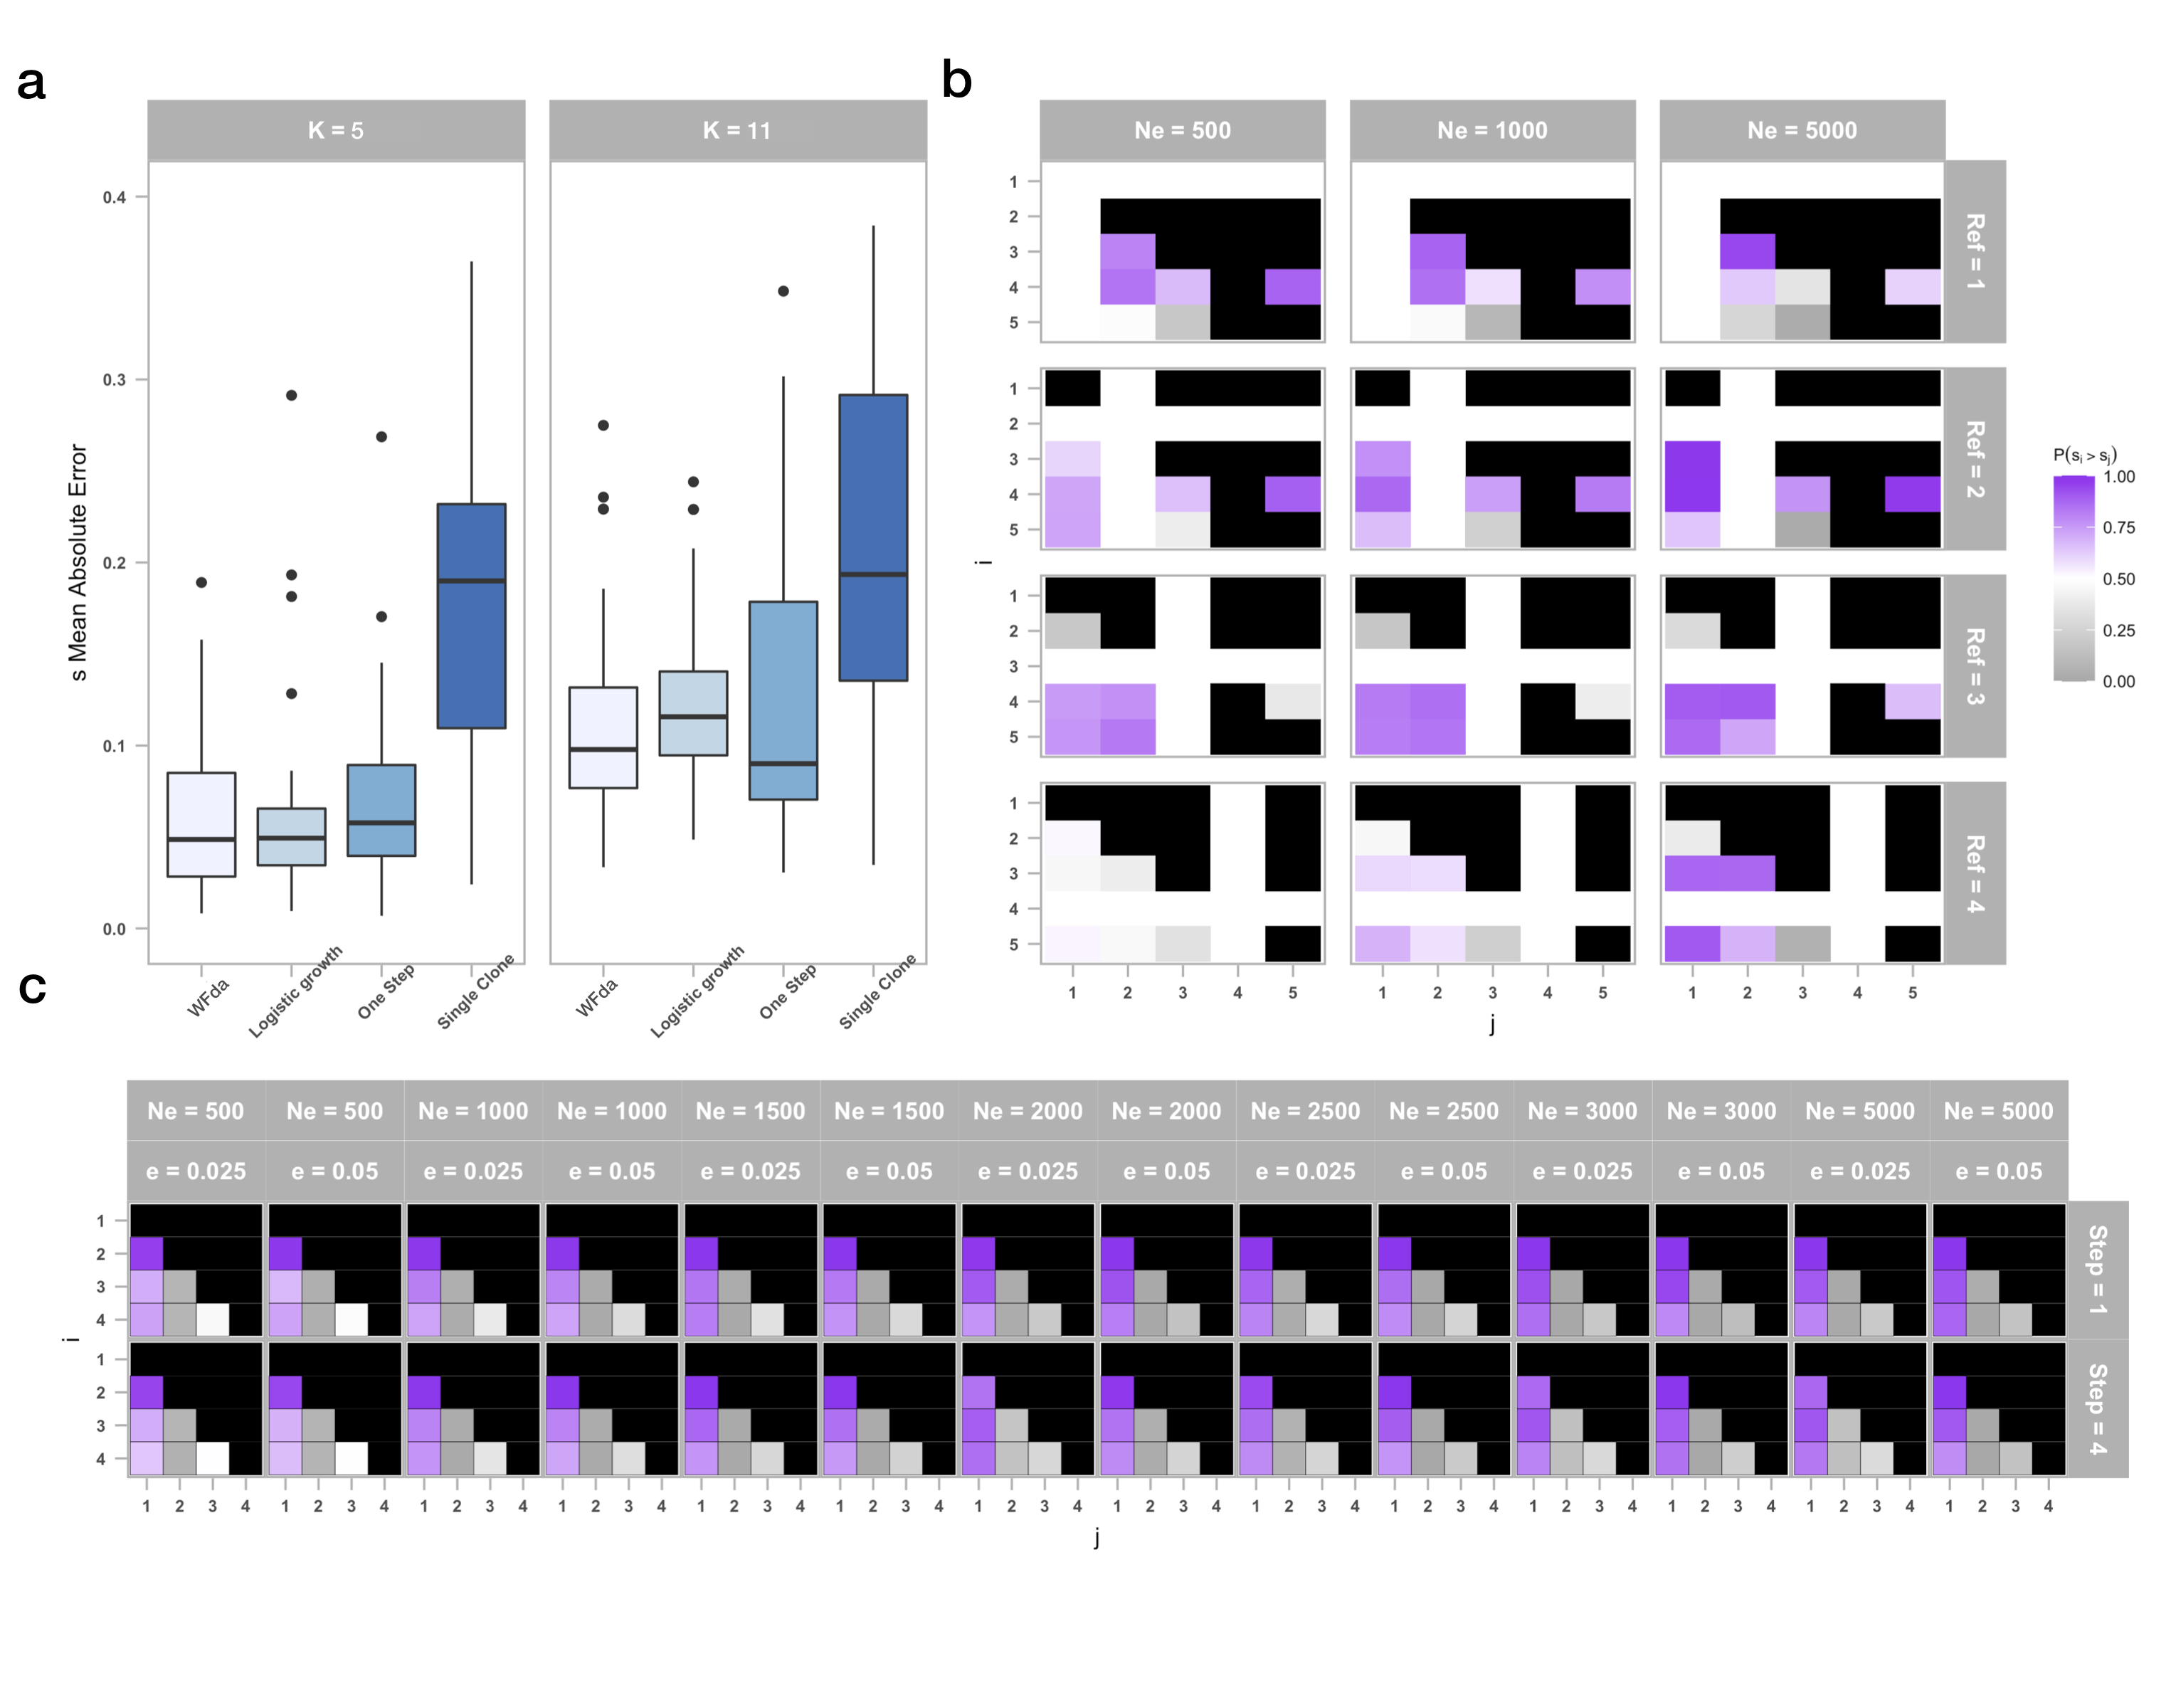
\includegraphics[width=\textwidth]{Figures/simulationspdx.png}
	
\caption[Simulation studies for the \texttt{fitClone} model]
	{\small
	\textbf{Simulation studies for the \texttt{fitClone} model.}
	  (a) Comparison to baseline methods for K = 5 clones (left) and K = 11 clones (right). (b) Posterior ordering of clones based on their inferred posterior selection coefficients across three values of effective population size (columns) and different choice of the reference clone (rows). (c) Posterior ordering of clones across different hyper parameters in the \texttt{fitClone} model. Effective population size in the range of 500 to 5,000 (top column), and observation error (bottom column). Minimum number of interpolations between two observations (rows).}
\label{fig:simulations}
\end{figure}


%-----------------------------------------------------------------


%---------------------------------------------------------------

\begin{figure}
\centering
  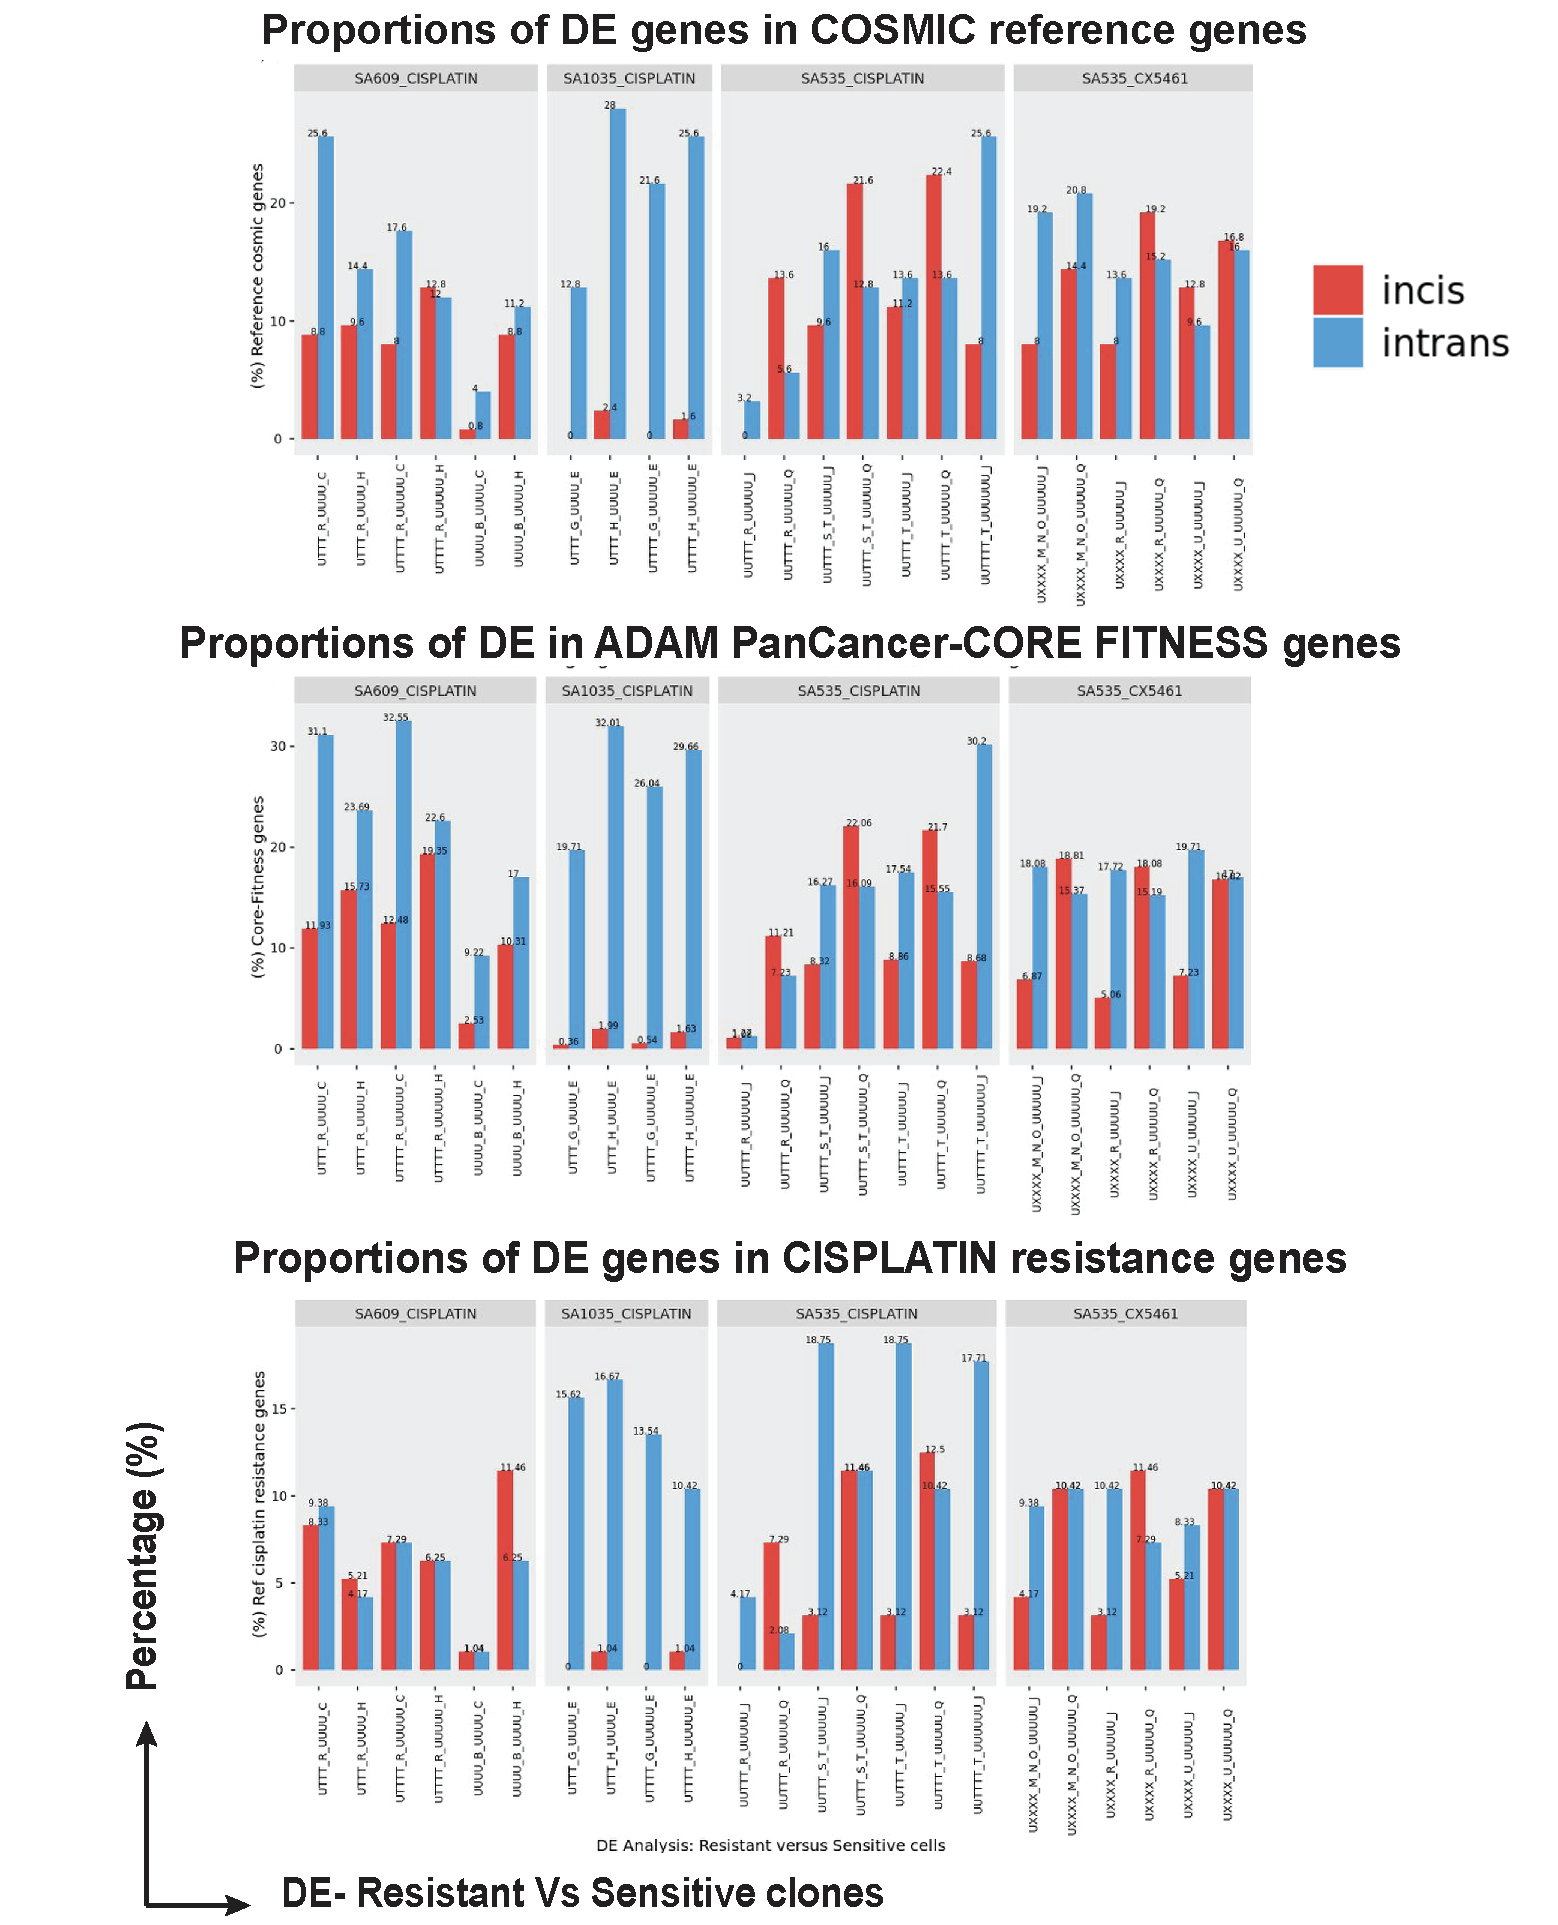
\includegraphics[width=\textwidth]{Figures/chap5/fig3_In_cispercentage.png}
	
\caption[Proportion of \textit{in cis} and \textit{in trans} regulated gene expression in scRNAseq data]
	{\small
	\textbf{Proportion of \textit{cis} and \textit{trans} regulated gene expression in scRNAseq data.}
	   Horizontal axis shows differential expression between two selected clones from all the three PDX treated and un-treated timeseries. Vertical axis gives percentage presence of genes \textit{in cis} or in trans. red bars represent in cis and blue bars represent in -trans regulated gene expression.
	   \textbf{(Upper)} This graph gives us percentage of genes by looking into the gene data set from COSMIC cancer gene dataset \cite{vogelstein2013cancer} that corresponds to our clone aware \ac{DE}.
	    \textbf{(Middle)} same like upper plot but looking into CORE FITNESS data set \cite{behan2019prioritization}.
	     \textbf{(Lower)} Same like above but looking into cisplatin related gene list curated from literature.
	    
	}
	\label{fig:fig3_In_cispercentage}
\end{figure}

%--------------------------------------------------------------------


\begin{figure}
\centering
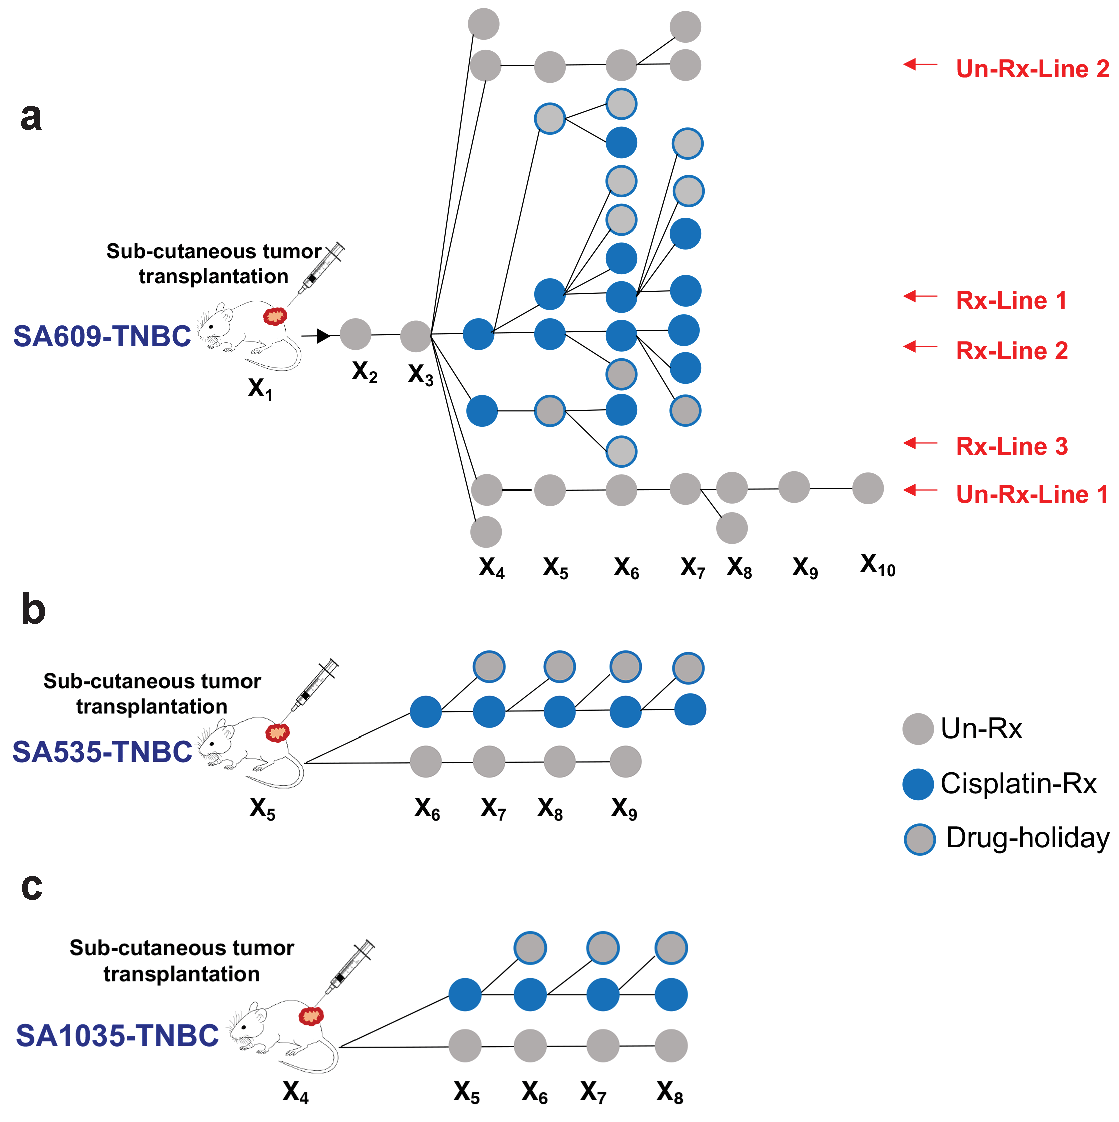
\includegraphics[width=\textwidth]{Figures/chap4/treatedtimeseriesmanuscript.pdf}
  \caption[TNBC PDX timeseries clonal dynamics under drug perturbations]
	{\small
	\textbf{TNBC PDX timeseries showing timepoint nodes smapled for single cell whole genome sequencing}
	     All nodes representing each PDX tumour were digested to acquire genomes of single cells (~200-600 cells/tumor). Extra replicate tumors at each time point are not shown in the diagram (n=2-4). Grey circles represent un-treated, blue represents Cisplatin treated and grey with blue outline presents drug-holiday samples 
	     \textbf{(a)} SA609-TNBC time series with replicates. DLP+ collected starting from X1 to X10 (Un-Rx line 1). Top grey branch indicating Un-Rx line 2. The middle three branches are cisplatin treated time series replicate branches 
	     \textbf{(b)} SA535-TNBC  showing the tumor nodes taken for DLP+ starting from X5 untreated  \textbf{(c)} SA1035-TNBC  showing the tumor nodes taken for DLP+ starting from X 4 untreated.}
     \label{fig:treatedtimeseriesmanuscript}

\end{figure}

%----------------------------------------------------------------------


 % Table generated by Excel2LaTeX from sheet 'Sheet1'
 \begin{table}[htbp]
   \centering
   \caption{Cisplatin related genes from last 10 years literature}
     \begin{tabular}{|l|l|l|l|r}
     
     \hline
     \multicolumn{4}{|l|}{Gene Names}  \\
     \hline
     
     VCAM1  & GCS    & BRCA2  & XAF1    \\
     VIM    & GST    & VDAC   & DYRK1B  \\
     SLC31A1 & MT     & BAX    & ERBB2 \\
     GST    & ERCC1  & BCL    & HSPs   \\
     HMGB   & MLH1   & BIRC5  & TMEM205 \\
     CTR1   & MSH2   & CPN    & PDGFR \\
     ATP7A  & POLH   & CASP   & IGF1R  \\
     ATP7B  & REV3   & MAPKs  & TRP14  \\
     MRP2   & REV7   & p63    & RAB7   \\
     GSH    & BRCA1  & TP53   & RAB8   \\
     \hline
     \end{tabular}%
   \label{tab:Cisplatinrelatedgenes}%
 \end{table}
 
 
 
\begin{figure}
\centering
  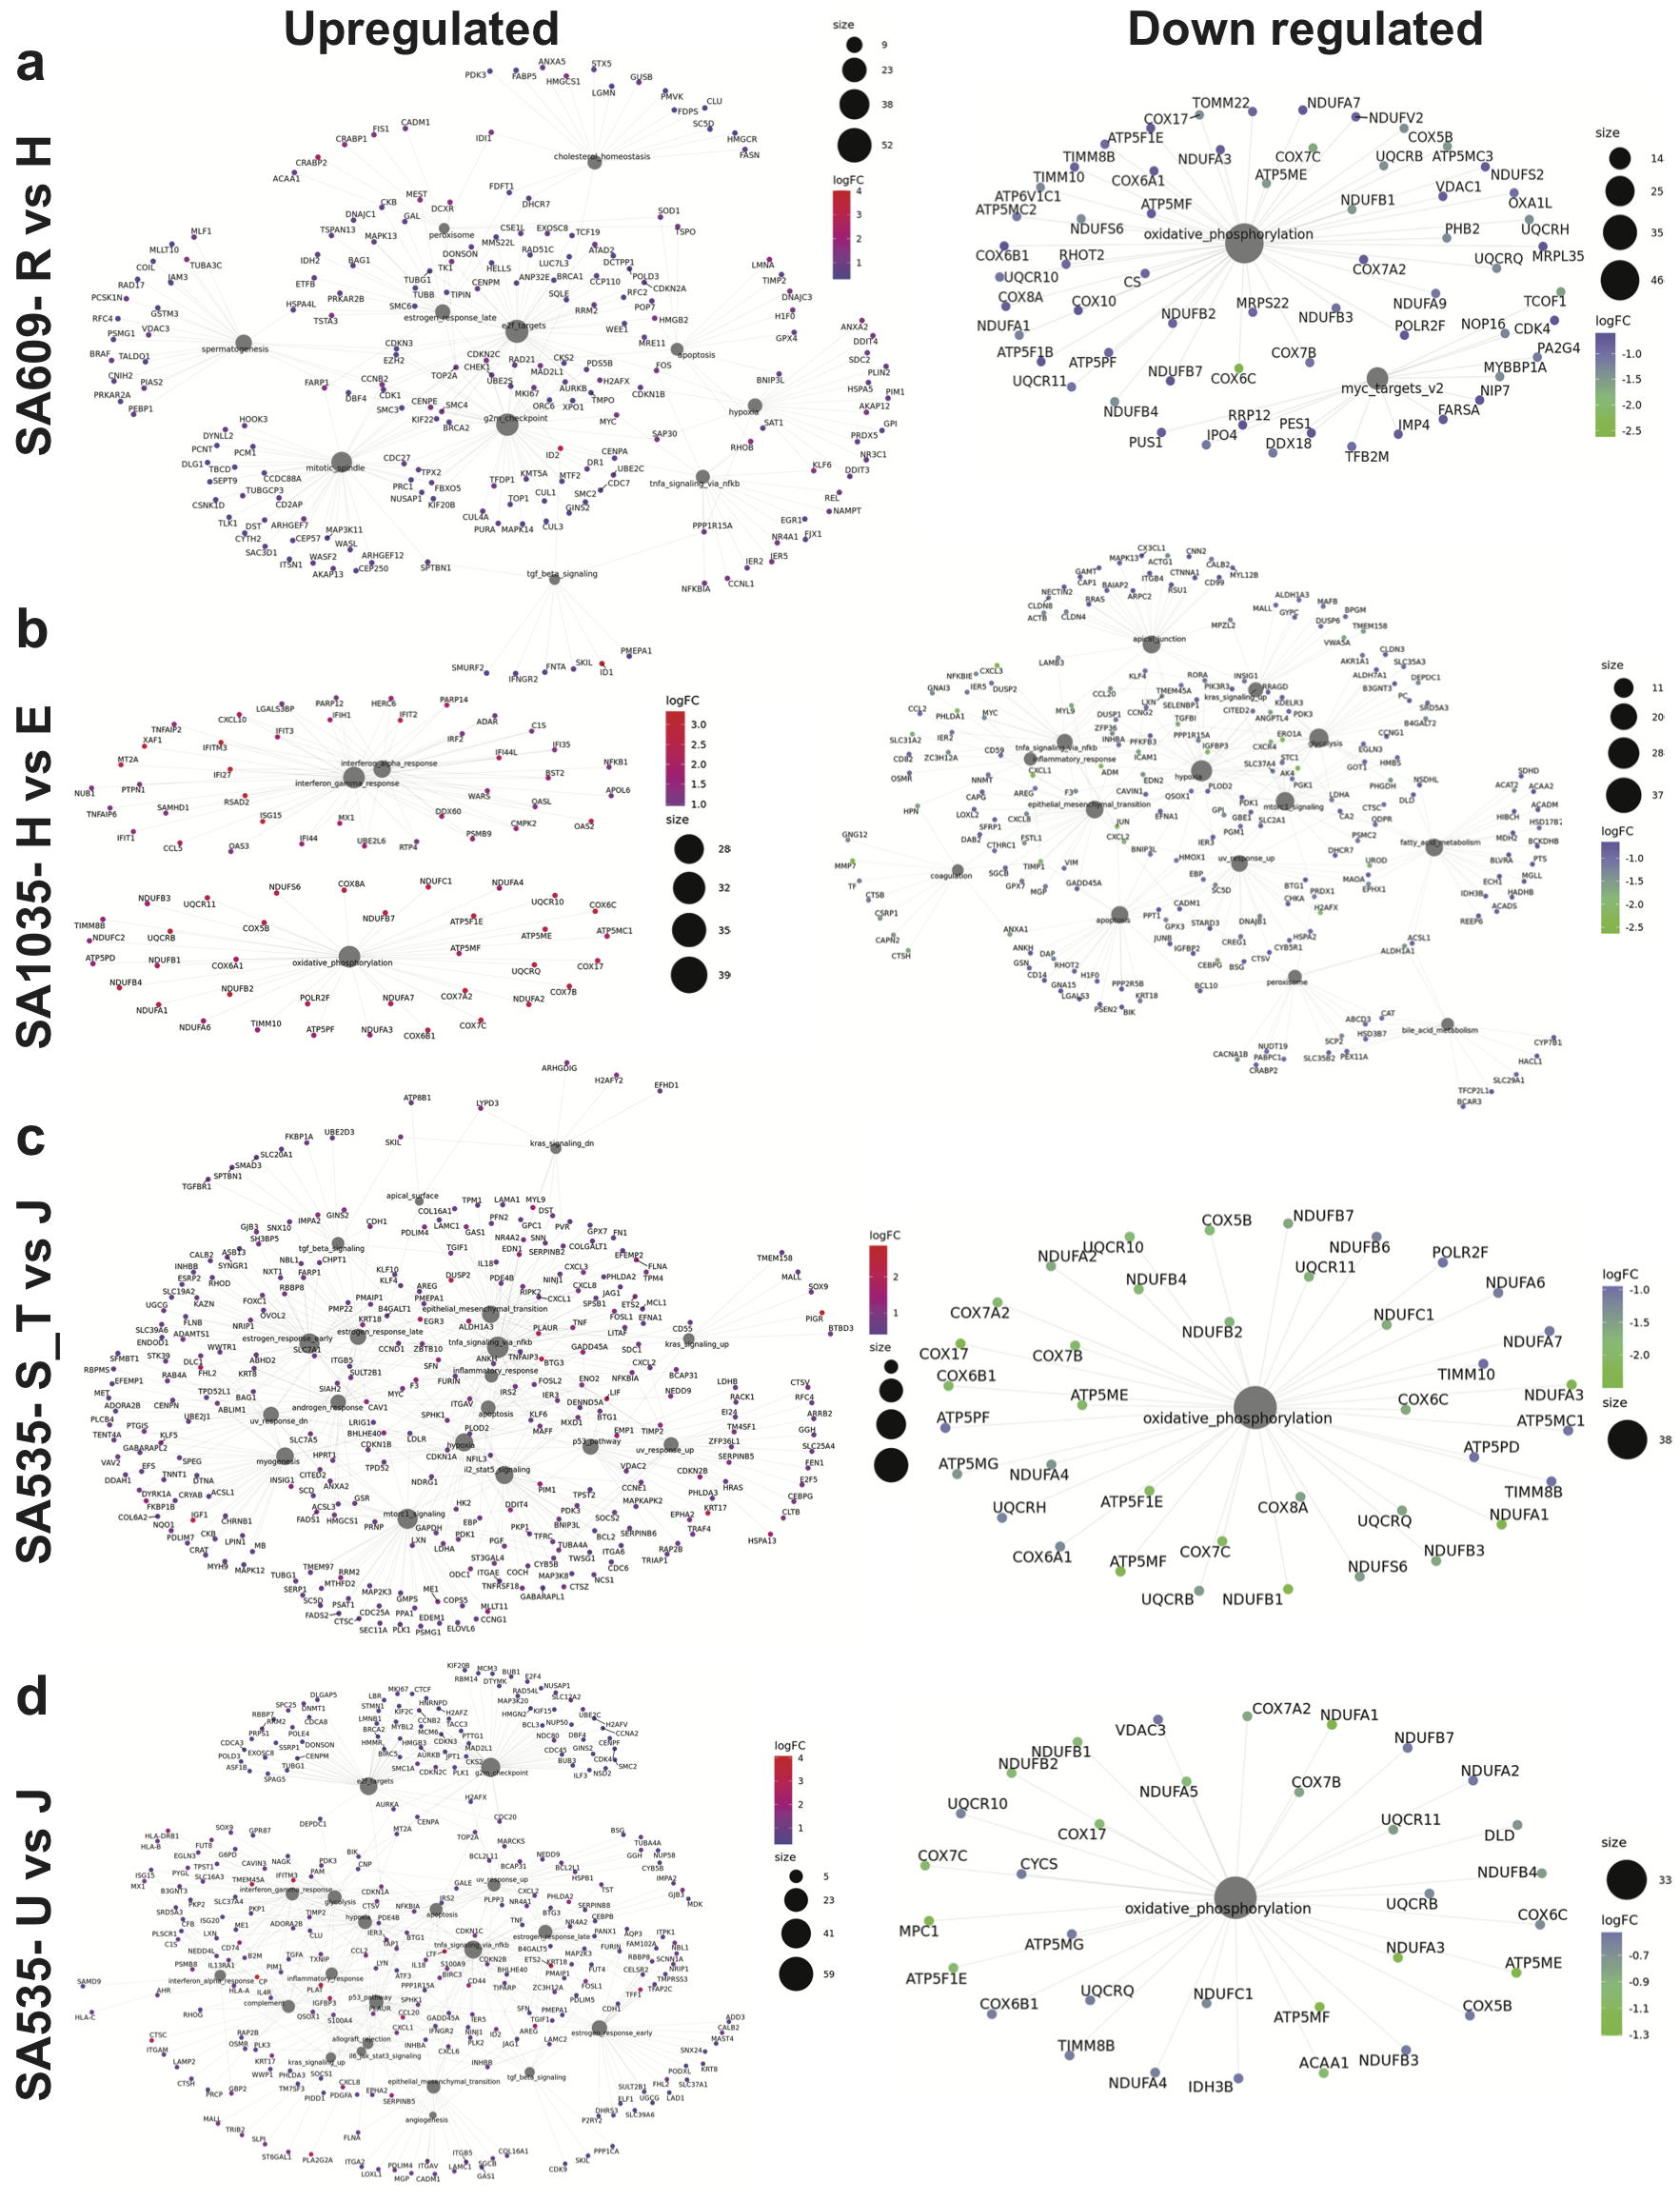
\includegraphics[width=\textwidth]{Figures/chap5/genenetworkanalysis .png}
\caption[DE of resistant and sensitive clonealign defined clones]
	{\small
	\textbf{Gene network analysis denoting connections of up-and-down regulated pathways across timeseries PDX}. Size of black circle indicates the number of genes, colour bars indicate the log fold change.
	\textbf{(a-d)} Genes in resistant vs sensitive clones of SA609, SA1035, SA535 (cisplatin and CX-5461 treated), respectively}
	  
	   	\label{fig:genenetworkanalysis}
\end{figure} 
 
 
 % Please add the following required packages to your document preamble:
% \usepackage{graphicx}
% \usepackage{lscape}
\begin{landscape}
\begin{table}[]
\caption{All PDX-TMA scoring of IHC staining}
\label{tab:my-table}
\resizebox{1.5\textwidth}{!}{%
\begin{tabular}{lllllllllllllllllllllllllllllllllllllllll}
Timeseries/TMA1 &
  Timepoints &
  Treatment status &
  ER intensity &
  ER \% &
  PR intensity &
  PR \% &
  HER 2 intensity &
  HER 2 \% &
  Ki67 intensity &
  Ki67 \% &
  EGFR intensity &
  EGFR \% &
  SMA intensity &
  SMA \% &
  CK8 intensity &
  CK8 \% &
  CK14 intensity &
  CK14 \% &
  CK5/6 intensity &
  CK5/6 \% &
  E-cad intensity &
  E-cad \% &
  comments &
   &
  vimentin intensity &
  vimentin \% &
  slug/snail intensity &
  slug/snail \% &
  twist intensity &
  twist \% &
  INPP4B intensity &
  INPP4B \% &
  Masson trichrome &
  comments &
   &
   &
   &
   &
   &
   \\
HER2+ &
  X1 &
  Un-Rx &
  0 &
  0 &
  0 &
  0 &
  1+ &
  30 &
  3+ &
  60 &
  0 &
  0 &
  3+ &
  0-1 &
  1+ &
  10 &
  3+ &
  80 &
  3+ &
  70 &
  0 &
  0 &
  HER2? &
   &
  0 &
  0 &
  1+ &
  70 &
  0 &
  0 &
  0 &
  0 &
  2+ &
  most tumor disappered in INPP4B restain &
   &
   &
   &
   &
   &
   \\
HER2+ &
  X2 &
  Un-Rx &
  0 &
  0 &
  0 &
  0 &
  1+ &
  30 &
  3+ &
  60 &
  0 &
  0 &
  3+ &
  5 &
  1+ &
  1-5 &
  3+ &
  60 &
  3+ &
  80 &
  0 &
  0 &
   &
   &
  3+ &
  0-1 &
  1+ &
  80 &
  0 &
  0 &
  1+ &
  1 &
  1+ &
   &
   &
   &
   &
   &
   &
   \\
HER2+ &
  X3 &
  Un-Rx &
  1+ &
  0-1 &
  0 &
  0 &
  2+ &
  30 &
  2+ &
  30 &
  0 &
  0 &
  3+ &
  1-5 &
  2+ &
  20 &
  3+ &
  20 &
  3+ &
  50 &
  0 &
  0 &
   &
   &
  3+ &
  0-1 &
  1+ &
  70 &
  0 &
  0 &
  1+ &
  0-1 &
  2+ &
   &
   &
   &
   &
   &
   &
   \\
HER2+ &
  X4 &
  Un-Rx &
  0 &
  0 &
  0 &
  0 &
  1+ &
  10 &
  3+ &
  70 &
  0 &
  0 &
  3+ &
  20 &
  1+ &
  1-5 &
  3+ &
  1-5 &
  3+ &
  20 &
  0 &
  0 &
   &
   &
  3+ &
  0-1 &
  2+ &
  70 &
  0 &
  0 &
  1+ &
  0-1 &
  1+ &
   &
   &
   &
   &
   &
   &
   \\
HER2+ &
  X5 &
  Un-Rx &
  0 &
  0 &
  0 &
  0 &
  0 &
  0 &
  3+ &
  70 &
  1+ &
  5 &
  3+ &
  1 &
  1+ &
  1-5 &
  2+ &
  1 &
  2+ &
  10 &
  3+ &
  60 &
  E-cad nega area artifact? &
   &
  3+ &
  0-1 &
  1+ &
  50 &
  0 &
  0 &
  1+ &
  0-1 &
  0 &
   &
   &
   &
   &
   &
   &
   \\
HER2+ &
  X6 &
  Un-Rx &
  0 &
  0 &
  0 &
  0 &
  1+ &
  10 &
  3+ &
  70 &
  1+ &
  5 &
  2+ &
  1-5 &
  1+ &
  1 &
  3+ &
  1 &
  2+ &
  10 &
  3+ &
  30 &
  E-cad nega area artifact? &
   &
  3+ &
  0-1 &
  1+ &
  60 &
  3+ &
  0-1 &
  1+ &
  0-1 &
  0 &
   &
   &
   &
   &
   &
   &
   \\
HER2+ &
  X7 &
  Un-Rx &
  0 &
  0 &
  0 &
  0 &
  1+ &
  5 &
  3+ &
  50 &
  2+ &
  5 &
  2+ &
  1 &
  1+ &
  0-1 &
  3+ &
  1-5 &
  2+ &
  10 &
  3+ &
  70 &
   &
   &
  3+ &
  0-1 &
  1+ &
  20 &
  0 &
  0 &
  0 &
  0 &
  1+ &
   &
   &
   &
   &
   &
   &
   \\
HER2+ &
  X8 &
  Un-Rx &
  0 &
  0 &
  0 &
  0 &
  0 &
  0 &
  2+ &
  30 &
  0 &
  0 &
  1+ &
  40 &
  1+ &
  1-5 &
  3+ &
  5 &
  1+ &
  10 &
  3+ &
  80 &
   &
   &
  2+ &
  1 &
  0 &
  0 &
  0 &
  0 &
  0 &
  0 &
  2+ &
   &
   &
   &
   &
   &
   &
   \\
HER2+ &
  X9 &
  Un-Rx &
  0 &
  0 &
  0 &
  0 &
  2+ &
  20 &
  3+ &
  50 &
  2+ &
  5 &
  2+ &
  0-1 &
  1+ &
  5 &
  3+ &
  1 &
  3+ &
  20 &
  3+ &
  100 &
   &
   &
  3+ &
  1 &
  2+ &
  80 &
  3+ &
  0-1 &
  1+ &
  0-1 &
  1+ &
   &
   &
   &
   &
   &
   &
   \\
HER2+ &
  X10 &
  Un-Rx &
  0 &
  0 &
  0 &
  0 &
  1+ &
  20 &
  3+ &
  70 &
  1+ &
  10 &
  3+ &
  30 &
  1+ &
  1 &
  3+ &
  1-5 &
  3+ &
  20 &
  3+ &
  100 &
   &
   &
  3+ &
  1 &
  2+ &
  80 &
  3+ &
  0-1 &
  1+ &
  0-1 &
  1+ &
   &
   &
   &
   &
   &
   &
   \\
 &
   &
   &
   &
   &
   &
   &
   &
   &
   &
   &
   &
   &
   &
   &
   &
   &
   &
   &
   &
   &
   &
   &
   &
   &
   &
   &
   &
   &
   &
   &
   &
   &
   &
   &
   &
   &
   &
   &
   &
   \\
TNBC-SA609 &
  X1 &
  Un-Rx &
  0 &
  0 &
  1+ &
  5 &
  0 &
  0 &
  3+ &
  80 &
  0 &
  0 &
  2+ &
  1 &
  0 &
  0 &
  1+ &
  0-1 &
  2+ &
  0-1 &
  0 &
  0 &
   &
   &
  3+ &
  20 &
  1+ &
  60 &
  2+ &
  0-1 &
  0 &
  0 &
  0 &
  INPP4B nuclear+ &
   &
   &
   &
   &
   &
   \\
TNBC-SA609 &
  X2 &
  Un-Rx &
  0 &
  0 &
  1+ &
  0-1 &
  0 &
  0 &
  3+ &
  80 &
  0 &
  0 &
  2+ &
  10 &
  0 &
  0 &
  1+ &
  0-1 &
  0 &
  0 &
  0 &
  0 &
  necrosis\textgreater{}\textgreater{}tumor CK14 back; strong false posi? &
   &
  3+ &
  05-Jan &
  2+ &
  80 &
  0 &
  0 &
  0 &
  0 &
  0 &
  necrosis\textgreater{}\textgreater{}tumor ,INPP4B nuclear+ &
   &
   &
   &
   &
   &
   \\
TNBC-SA609 &
  X3 &
  Un-Rx &
  0 &
  0 &
  1+ &
  10 &
  0 &
  0 &
  3+ &
  70 &
  1+ &
  30 &
  2+ &
  0-1 &
  0 &
  0 &
  1+ &
  1-5 &
  0 &
  0 &
  0 &
  0 &
   &
   &
  3+ &
  5 &
  2+ &
  80 &
  3+ &
  0-1 &
  0 &
  0 &
  1+ &
  INPP4B nuclear+ &
   &
   &
   &
   &
   &
   \\
TNBC-SA609 &
  X4 &
  Un-Rx &
  0 &
  0 &
  1+ &
  10 &
  0 &
  0 &
  3+ &
  60 &
  1+ &
  30 &
  2+ &
  0-1 &
  0 &
  0 &
  1+ &
  0-1 &
  0 &
  0 &
  0 &
  0 &
   &
   &
  3+ &
  20 &
  2+ &
  90 &
  3+ &
  0-1 &
  0 &
  0 &
  2+ &
  INPP4B nuclear+ &
   &
   &
   &
   &
   &
   \\
TNBC-SA609 &
  X5 &
  Un-Rx &
  0 &
  0 &
  0 &
  0 &
  0 &
  0 &
  3+ &
  60 &
  1+ &
  10 &
  2+ &
  0-1 &
  0 &
  0 &
  1+ &
  0-1 &
  0 &
  0 &
  0 &
  0 &
   &
   &
  3+ &
  30 &
  2+ &
  80 &
  0 &
  0 &
  0 &
  0 &
  2+ &
  INPP4B nuclear+ &
   &
   &
   &
   &
   &
   \\
TNBC-SA609 &
  X6 &
  Un-Rx &
  0 &
  0 &
  1+ &
  0-1 &
  0 &
  0 &
  2+ &
  70 &
  3+ &
  40 &
  3+ &
  0-1 &
  1+ &
  0-1 &
  1+ &
  1 &
  0 &
  0 &
  0 &
  0 &
   &
   &
  3+ &
  5 &
  2+ &
  90 &
  3+ &
  0-1 &
  0 &
  0 &
  2+ &
  INPP4B nuclear+ &
   &
   &
   &
   &
   &
   \\
TNBC-SA609 &
  X7 &
  Un-Rx &
  0 &
  0 &
  1+ &
  0-1 &
  0 &
  0 &
  2+ &
  70 &
  3+ &
  20 &
  3+ &
  0-1 &
  0 &
  0 &
  1+ &
  0-1 &
  0 &
  0 &
  0 &
  0 &
   &
   &
  3+ &
  10 &
  2+ &
  90 &
  3+ &
  0-1 &
  0 &
  0 &
  1+ &
  masson: collagen (blue) under the squre,INPP4B nuclear+ &
   &
   &
   &
   &
   &
   \\
TNBC-SA609 &
  X8 &
  Un-Rx &
  0 &
  0 &
  1+ &
  0-1 &
  0 &
  0 &
  3+ &
  70 &
  3+ &
  50 &
  3+ &
  0-1 &
  0 &
  0 &
  1+ &
  0-1 &
  0 &
  0 &
  0 &
  0 &
   &
   &
  3+ &
  10 &
  2+ &
  80 &
  3+ &
  0-1 &
  0 &
  0 &
  2+ &
  INPP4B nuclear+ &
   &
   &
   &
   &
   &
   \\
TNBC-SA609 &
  X9 &
  Un-Rx &
  0 &
  0 &
  1+ &
  0-1 &
  0 &
  0 &
  3+ &
  80 &
  3+ &
  20 &
  3+ &
  0-1 &
  0 &
  0 &
  1+ &
  0-1 &
  0 &
  0 &
  0 &
  0 &
   &
   &
  3+ &
  70 &
  2+ &
  90 &
  3+ &
  0-1 &
  0 &
  0 &
  0 &
  INPP4B nuclear+ &
   &
   &
   &
   &
   &
   \\
TNBC-SA609 &
  X10 &
  Un-Rx &
  0 &
  0 &
  1+ &
  0-1 &
  0 &
  0 &
  3+ &
  70 &
  3+ &
  60 &
  3+ &
  5 &
  0 &
  0 &
  1+ &
  1 &
  0 &
  0 &
  0 &
  0 &
   &
   &
  3+ &
  5 &
  2+ &
  80 &
  3+ &
  0-1 &
  0 &
  0 &
  2+ &
  INPP4B nuclear+ &
   &
   &
   &
   &
   &
   \\
 &
   &
   &
   &
   &
   &
   &
   &
   &
   &
   &
   &
   &
   &
   &
   &
   &
   &
   &
   &
   &
   &
   &
   &
   &
   &
   &
   &
   &
   &
   &
   &
   &
   &
   &
   &
   &
   &
   &
   &
   \\
 &
   &
   &
   &
   &
   &
   &
   &
   &
   &
   &
   &
   &
   &
   &
   &
   &
   &
   &
   &
   &
   &
   &
   &
   &
   &
   &
   &
   &
   &
   &
   &
   &
   &
   &
   &
   &
   &
   &
   &
   \\
Timeseries/TMA2 &
  Timepoints &
  Treatment status &
  Block ID &
  ER intensity &
  ER \% &
  PR intensity &
  PR \% &
  HER 2 intensity &
  HER 2 \% &
  Ki67 intensity &
  Ki67 \% &
  EGFR intensity &
  EGFR \% &
  SMA intensity &
  SMA \% &
  CK8(CAM5.2) intensity &
  CK8(CAM5.2) \% &
  CK14 intensity &
  CK14 \% &
  CK5/6 intensity &
  CK5/6 \% &
  E-cad intensity &
  E-cad \% &
  vimentin intensity &
  vimentin \% &
  slug/snail intensity &
  slug/snail \% &
  twist intensity &
  twist \% &
  INPP4B intensity &
  INPP4B \% &
  Masson trichrome &
  PAS\&CD31 &
  comments &
   &
   &
   &
   &
   &
   \\
TNBC-SA609 &
  X4 &
  Un-Rx &
  3080 &
  0 &
  0 &
  0 &
  0 &
  0 &
  0 &
  3+ &
  45 &
  1+ &
  50 &
  0 &
  0 &
  0 &
  0 &
  0 &
  0 &
  0 &
  0 &
  0 &
  0 &
  3+ &
  40 &
  2+ &
  95 &
  0 &
  0 &
  0 &
  0 &
  1+ &
  0 &
   &
   &
   &
   &
   &
   &
   \\
TNBC-SA609 &
  X5 &
  Un-Rx &
  3223 &
  0 &
  0 &
  0 &
  0 &
  0 &
  0 &
  3+ &
  50 &
  1+ &
  40 &
  0 &
  0 &
  0 &
  0 &
  0 &
  0 &
  0 &
  0 &
  0 &
  0 &
  3+ &
  20 &
  2+ &
  95 &
  0 &
  0 &
  0 &
  0 &
  1+ &
  0 &
   &
   &
   &
   &
   &
   &
   \\
TNBC-SA609 &
  X6 &
  Un-Rx &
  3447 &
  0 &
  0 &
  0 &
  0 &
  0 &
  0 &
  3+ &
  45 &
  2+ &
  30 &
  3+ &
  0-1 &
  0 &
  0 &
  0 &
  0 &
  0 &
  0 &
  0 &
  0 &
  3+ &
  40 &
  2+ &
  95 &
  0 &
  0 &
  0 &
  0 &
  1+ &
  0 &
   &
   &
   &
   &
   &
   &
   \\
TNBC-SA609 &
  X4 &
  Rx &
  3083 &
  0 &
  0 &
  0 &
  0 &
  0 &
  0 &
  3+ &
  60 &
  1+ &
  60 &
  0 &
  0 &
  0 &
  0 &
  0 &
  0 &
  0 &
  0 &
  0 &
  0 &
  3+ &
  15 &
  2+ &
  95 &
  0 &
  0 &
  1+ &
  0-1 &
  2+ &
  2 &
   &
   &
   &
   &
   &
   &
   \\
TNBC-SA609 &
  X4 &
  Rx &
  3084 &
  0 &
  0 &
  0 &
  0 &
  0 &
  0 &
  3+ &
  70 &
  1+ &
  70 &
  0 &
  0 &
  0 &
  0 &
  0 &
  0 &
  0 &
  0 &
  0 &
  0 &
  3+ &
  20 &
  2+ &
  95 &
  0 &
  0 &
  1+ &
  0-1 &
  1+ &
  0 &
   &
   &
   &
   &
   &
   &
   \\
TNBC-SA609 &
  X5 &
  Rx &
  3230 &
  0 &
  0 &
  0 &
  0 &
  0 &
  0 &
  3+ &
  45 &
  1+ &
  50 &
  0 &
  0 &
  0 &
  0 &
  0 &
  0 &
  0 &
  0 &
  0 &
  0 &
  3+ &
  20 &
  2+ &
  95 &
  0 &
  0 &
  1+ &
  0-1 &
  1+ &
  1 &
   &
   &
   &
   &
   &
   &
   \\
TNBC-SA609 &
  X5 &
  dh &
  3231 &
  0 &
  0 &
  0 &
  0 &
  0 &
  0 &
  3+ &
  35 &
  1+ &
  75 &
  0 &
  0 &
  0 &
  0 &
  0 &
  0 &
  0 &
  0 &
  0 &
  0 &
  3+ &
  25 &
  2+ &
  95 &
  0 &
  0 &
  0 &
  0 &
  1+ &
  1 &
   &
   &
   &
   &
   &
   &
   \\
TNBC-SA609 &
  X5 &
  Rx-recur &
  3235 &
  0 &
  0 &
  0 &
  0 &
  0 &
  0 &
  3+ &
  35 &
  2+ &
  50 &
  0 &
  0 &
  0 &
  0 &
  0 &
  0 &
  0 &
  0 &
  0 &
  0 &
  3+ &
  20 &
  2+ &
  95 &
  0 &
  0 &
  0 &
  0 &
  1+ &
  2 &
   &
   &
   &
   &
   &
   &
   \\
TNBC-SA609 &
  X6 &
  Rx &
  3400 &
  0 &
  0 &
  0 &
  0 &
  0 &
  0 &
  3+ &
  35 &
  1+ &
  40 &
  0 &
  0 &
  0 &
  0 &
  0 &
  0 &
  0 &
  0 &
  0 &
  0 &
  3+ &
  0-1 &
  2+ &
  95 &
  0 &
  0 &
  0 &
  0 &
  3+ &
  1 &
   &
   &
   &
   &
   &
   &
   \\
TNBC-SA609 &
  X6 &
  dh &
  3401 &
  0 &
  0 &
  0 &
  0 &
  0 &
  0 &
  3+ &
  30 &
  1+ &
  10 &
  0 &
  0 &
  0 &
  0 &
  0 &
  0 &
  0 &
  0 &
  0 &
  0 &
  3+ &
  0-1 &
  2+ &
  95 &
  0 &
  0 &
  0 &
  0 &
  2+ &
  1* &
  *insufficient material for evaluate VM due to lot of necrosis &
   &
   &
   &
   &
   &
   \\
TNBC-SA609 &
  X6 &
  Rx &
  3404 &
  0 &
  0 &
  0 &
  0 &
  0 &
  0 &
  3+ &
  35 &
  1+ &
  40 &
  0 &
  0 &
  0 &
  0 &
  0 &
  0 &
  0 &
  0 &
  0 &
  0 &
  3+ &
  5 &
  2+ &
  95 &
  0 &
  0 &
  0 &
  0 &
  2+ &
  0 &
   &
   &
   &
   &
   &
   &
   \\
TNBC-SA609 &
  X7 &
  Rx &
  3505 &
  0 &
  0 &
  0 &
  0 &
  0 &
  0 &
  3+ &
  50 &
  1+ &
  40 &
  0 &
  0 &
  0 &
  0 &
  0 &
  0 &
  0 &
  0 &
  0 &
  0 &
  3+ &
  5-10 &
  2+ &
  95 &
  0 &
  0 &
  0 &
  0 &
  1+ &
  2 &
   &
   &
   &
   &
   &
   &
   \\
TNBC-SA609 &
  X7 &
  Rx &
  3506 &
  0 &
  0 &
  1+ &
  0-1 &
  0 &
  0 &
  3+ &
  60 &
  1+ &
  60 &
  0 &
  0 &
  0 &
  0 &
  0 &
  0 &
  0 &
  0 &
  0 &
  0 &
  3+ &
  5-10 &
  2+ &
  95 &
  0 &
  0 &
  0 &
  0 &
  1+ &
  0 &
   &
   &
   &
   &
   &
   &
   \\
TNBC-SA609 &
  X7 &
  dh &
  3510 &
  0 &
  0 &
  1+ &
  0-1 &
  0 &
  0 &
  3+ &
  45 &
  1+ &
  40 &
  0 &
  0 &
  0 &
  0 &
  0 &
  0 &
  0 &
  0 &
  0 &
  0 &
  3+ &
  5-10 &
  2+ &
  95 &
  0 &
  0 &
  0 &
  0 &
  1+ &
  2 &
   &
   &
   &
   &
   &
   &
   \\
TNBC-SA609 &
  X5 &
  Rx &
  3226 &
  0 &
  0 &
  0 &
  0 &
  0 &
  0 &
  3+ &
  45 &
  1+ &
  35 &
  0 &
  0 &
  0 &
  0 &
  0 &
  0 &
  0 &
  0 &
  0 &
  0 &
  3+ &
  15 &
  2+ &
  95 &
  0 &
  0 &
  1+ &
  1 &
  2+ &
  2 &
   &
   &
   &
   &
   &
   &
   \\
TNBC-SA609 &
  X6 &
  Rx &
  3387 &
  0 &
  0 &
  0 &
  0 &
  0 &
  0 &
  3+ &
  50 &
  1+ &
  50 &
  0 &
  0 &
  0 &
  0 &
  0 &
  0 &
  0 &
  0 &
  0 &
  0 &
  3+ &
  5-10 &
  2+ &
  95 &
  0 &
  0 &
  1+ &
  1 &
  1+ &
  2 &
   &
   &
   &
   &
   &
   &
   \\
TNBC-SA609 &
  X7 &
  Rx &
  3573 &
  0 &
  0 &
  0 &
  0 &
  0 &
  0 &
  3+ &
  90 &
  3+ &
  5 &
  0 &
  0 &
  0 &
  0 &
  0 &
  0 &
  0 &
  0 &
  0 &
  0 &
  2+ &
  15 &
  2+ &
  95 &
  0 &
  0 &
  1+ &
  1 &
  1+ &
  1 &
   &
   &
   &
   &
   &
   &
   \\
TNBC-SA609 &
  X7 &
  Rx &
  3578 &
  0 &
  0 &
  0 &
  0 &
  0 &
  0 &
  3+ &
  90 &
  1+ &
  10 &
  0 &
  0 &
  0 &
  0 &
  0 &
  0 &
  0 &
  0 &
  0 &
  0 &
  2+ &
  20 &
  2+ &
  95 &
  0 &
  0 &
  1+ &
  1 &
  1+ &
  2 &
   &
   &
   &
   &
   &
   &
   \\
TNBC-SA609 &
  X7 &
  dh &
  3508 &
  0 &
  0 &
  0 &
  0 &
  0 &
  0 &
  3+ &
  35 &
  1+ &
  35 &
  0 &
  0 &
  0 &
  0 &
  0 &
  0 &
  0 &
  0 &
  0 &
  0 &
  3+ &
  15 &
  2+ &
  95 &
  0 &
  0 &
  1+ &
  0-1 &
  1+ &
  0 &
   &
   &
   &
   &
   &
   &
   \\
TNBC-SA609 &
  X7 &
  dh &
  3577 &
  0 &
  0 &
  0 &
  0 &
  0 &
  0 &
  3+ &
  80 &
  1+ &
  5-10 &
  0 &
  0 &
  0 &
  0 &
  0 &
  0 &
  0 &
  0 &
  0 &
  0 &
  2+ &
  20 &
  2+ &
  95 &
  0 &
  0 &
  1+ &
  1 &
  1+ &
  0 &
   &
   &
   &
   &
   &
   &
   \\
 &
   &
   &
   &
   &
   &
   &
   &
   &
   &
   &
   &
   &
   &
   &
   &
   &
   &
   &
   &
   &
   &
   &
   &
   &
   &
   &
   &
   &
   &
   &
   &
   &
   &
   &
   &
   &
   &
   &
   &
   \\
TNBC-SA1035 &
  X4 &
  Un-Rx &
  2879 &
  1+ &
  0-1 &
  0 &
  0 &
  0 &
  0 &
  3+ &
  65 &
  3+ &
  100 &
  0 &
  0 &
  1+ &
  25 &
  3+ &
  5-10 &
  2+ &
  10 &
  3+ &
  100 &
  3+ &
  30 &
  2+ &
  95 &
  0 &
  0 &
  0 &
  0 &
  2+ &
  0 &
   &
   &
   &
   &
   &
   &
   \\
TNBC-SA1035 &
  X5 &
  Un-Rx &
  3021 &
  1+ &
  0-1 &
  0 &
  0 &
  0 &
  0 &
  3+ &
  50 &
  3+ &
  100 &
  0 &
  0 &
  1+ &
  5 &
  3+ &
  10 &
  2+ &
  10 &
  3+ &
  100 &
  3+ &
  20 &
  2+ &
  95 &
  0 &
  0 &
  0 &
  0 &
  2+ &
  0 &
   &
   &
   &
   &
   &
   &
   \\
TNBC-SA1035 &
  X6 &
  Un-Rx &
  3216 &
  1+ &
  0-1 &
  0 &
  0 &
  0 &
  0 &
  2+ &
  65 &
  3+ &
  100 &
  0 &
  0 &
  2+ &
  5 &
  3+ &
  0-1 &
  2+ &
  0-1 &
  3+ &
  100 &
  3+ &
  15 &
  2+ &
  95 &
  0 &
  0 &
  0 &
  0 &
  2+ &
  0 &
   &
   &
   &
   &
   &
   &
   \\
TNBC-SA1035 &
  X7 &
  Un-Rx &
  3502 &
  1+ &
  0-1 &
  0 &
  0 &
  0 &
  0 &
  3+ &
  70 &
  3+ &
  100 &
  0 &
  0 &
  1+ &
  5 &
  3+ &
  5 &
  2+ &
  10 &
  3+ &
  100 &
  3+ &
  20 &
  2+ &
  95 &
  0 &
  0 &
  0 &
  0 &
  2+ &
  0 &
   &
   &
   &
   &
   &
   &
   \\
TNBC-SA1035 &
  X8 &
  Un-Rx &
  3631 &
  1+ &
  0-1 &
  0 &
  0 &
  0 &
  0 &
  3+ &
  80 &
  3+ &
  100 &
  0 &
  0 &
  1+ &
  1-5 &
  3+ &
  0-1 &
  2+ &
  1 &
  3+ &
  100 &
  3+ &
  20 &
  2+ &
  95 &
  0 &
  0 &
  0 &
  0 &
  2+ &
  1 &
   &
   &
   &
   &
   &
   &
   \\
TNBC-SA1035 &
  X5 &
  Rx &
  3015 &
  1+ &
  0-1 &
  0 &
  0 &
  0 &
  0 &
  3+ &
  50 &
  3+ &
  95 &
  0 &
  0 &
  2+ &
  70 &
  3+ &
  10 &
  3+ &
  40 &
  3+ &
  100 &
  3+ &
  35 &
  2+ &
  95 &
  0 &
  0 &
  0 &
  0 &
  3+ &
  1 &
   &
   &
   &
   &
   &
   &
   \\
TNBC-SA1035 &
  X6 &
  dh &
  3209 &
  1+ &
  0-1 &
  0 &
  0 &
  0 &
  0 &
  3+ &
  60 &
  3+ &
  100 &
  0 &
  0 &
  2+ &
  5 &
  3+ &
  1 &
  2+ &
  10 &
  3+ &
  100 &
  3+ &
  20 &
  2+ &
  95 &
  0 &
  0 &
  0 &
  0 &
  3+ &
  1 &
   &
   &
   &
   &
   &
   &
   \\
TNBC-SA1035 &
  X6 &
  Rx &
  3211 &
  1+ &
  0-1 &
  0 &
  0 &
  0 &
  0 &
  3+ &
  50 &
  3+ &
  100 &
  0 &
  0 &
  2+ &
  20 &
  3+ &
  1 &
  2+ &
  30 &
  3+ &
  100 &
  3+ &
  10 &
  2+ &
  95 &
  0 &
  0 &
  1+ &
  0-1 &
  3+ &
  1 &
   &
   &
   &
   &
   &
   &
   \\
TNBC-SA1035 &
  X7 &
  Rx &
  3338 &
  1+ &
  0-1 &
  0 &
  0 &
  0 &
  0 &
  3+ &
  80 &
  3+ &
  100 &
  0 &
  0 &
  1+ &
  5 &
  3+ &
  1-5 &
  2+ &
  15 &
  3+ &
  100 &
  3+ &
  10 &
  2+ &
  95 &
  0 &
  0 &
  1+ &
  0-1 &
  2+ &
  0 &
   &
   &
   &
   &
   &
   &
   \\
TNBC-SA1035 &
  X7 &
  dh &
  3340 &
  1+ &
  0-1 &
  0 &
  0 &
  0 &
  0 &
  3+ &
  60 &
  3+ &
  100 &
  0 &
  0 &
  2+ &
  5 &
  3+ &
  1 &
  2+ &
  10 &
  3+ &
  100 &
  3+ &
  20 &
  2+ &
  95 &
  0 &
  0 &
  0 &
  0 &
  3+ &
  1 &
   &
   &
   &
   &
   &
   &
   \\
TNBC-SA1035 &
  X8 &
  Rx &
  3425 &
  1+ &
  0-1 &
  0 &
  0 &
  0 &
  0 &
  3+ &
  70 &
  3+ &
  100 &
  0 &
  0 &
  1+ &
  5 &
  3+ &
  1 &
  2+ &
  5 &
  3+ &
  100 &
  3+ &
  10 &
  2+ &
  95 &
  0 &
  0 &
  1+ &
  1 &
  2+ &
  0 &
   &
   &
   &
   &
   &
   &
   \\
 &
   &
   &
   &
   &
   &
   &
   &
   &
   &
   &
   &
   &
   &
   &
   &
   &
   &
   &
   &
   &
   &
   &
   &
   &
   &
   &
   &
   &
   &
   &
   &
   &
   &
   &
   &
   &
   &
   &
   &
   \\
TNBC-SA535 &
  X6 &
  Un-Rx &
  3099 &
  0 &
  0 &
  0 &
  0 &
  0 &
  0 &
  3+ &
  25 &
  3+ &
  90 &
  0 &
  0 &
  2+ &
  65 &
  0 &
  0 &
  2+ &
  1-5 &
  3+ &
  100 &
  3+ &
  60 &
  2+ &
  95 &
  0 &
  0 &
  0 &
  0 &
  2+ &
  no core &
   &
   &
   &
   &
   &
   &
   \\
TNBC-SA535 &
  X7 &
  Un-Rx &
  3448 &
  0 &
  0 &
  0 &
  0 &
  0 &
  0 &
  3+ &
  30 &
  3+ &
  100 &
  0 &
  0 &
  2+ &
  15 &
  0 &
  0 &
  2+ &
  0-1 &
  3+ &
  100 &
  3+ &
  80 &
  2+ &
  95 &
  0 &
  0 &
  0 &
  0 &
  2+ &
  no core &
   &
   &
   &
   &
   &
   &
   \\
TNBC-SA535 &
  X6 &
  Rx &
  3101 &
  1+ &
  0-1 &
  0 &
  0 &
  0 &
  0 &
  3+ &
  35 &
  2+ &
  95 &
  0 &
  0 &
  2+ &
  80 &
  3+ &
  1 &
  2+ &
  5 &
  3+ &
  100 &
  3+ &
  40 &
  2+ &
  95 &
  0 &
  0 &
  1+ &
  1 &
  2+ &
  2 &
   &
   &
   &
   &
   &
   &
   \\
TNBC-SA535 &
  X7 &
  Rx-cis &
  3304 &
  0 &
  0 &
  0 &
  0 &
  0 &
  0 &
  3+ &
  35 &
  2+ &
  80 &
  0 &
  0 &
  2+ &
  95 &
  3+ &
  0-1 &
  2+ &
  1 &
  3+ &
  100 &
  3+ &
  25 &
  2+ &
  95 &
  0 &
  0 &
  1+ &
  0-1 &
  2+ &
  1 &
   &
   &
   &
   &
   &
   &
   \\
TNBC-SA535 &
  X7 &
  dh-cis &
  3305 &
  0 &
  0 &
  0 &
  0 &
  0 &
  0 &
  3+ &
  35 &
  2+ &
  90 &
  0 &
  0 &
  3+ &
  95 &
  3+ &
  1 &
  2+ &
  5 &
  3+ &
  100 &
  3+ &
  15 &
  2+ &
  95 &
  0 &
  0 &
  2+ &
  1 &
  2+ &
  1 &
   &
   &
   &
   &
   &
   &
   \\
TNBC-SA535 &
  X8 &
  Rx-cis &
  3431 &
  1+ &
  0-1 &
  0 &
  0 &
  0 &
  0 &
  3+ &
  45 &
  2+ &
  95 &
  0 &
  0 &
  2+ &
  95 &
  3+ &
  0-1 &
  2+ &
  5 &
  3+ &
  100 &
  3+ &
  65 &
  2+ &
  95 &
  0 &
  0 &
  1+ &
  1 &
  2+ &
  1 &
   &
   &
   &
   &
   &
   &
   \\
TNBC-SA535 &
  X8 &
  dh-cis &
  3434 &
  1+ &
  1 &
  0 &
  0 &
  0 &
  0 &
  3+ &
  35 &
  2+ &
  85 &
  0 &
  0 &
  2+ &
  95 &
  3+ &
  1 &
  2+ &
  10 &
  3+ &
  100 &
  3+ &
  55 &
  2+ &
  95 &
  0 &
  0 &
  1+ &
  0-1 &
  2+ &
  0 &
   &
   &
   &
   &
   &
   &
   \\
TNBC-SA535 &
  X9 &
  dh-cis &
  3616 &
  1+ &
  1 &
  0 &
  0 &
  0 &
  0 &
  3+ &
  40 &
  2+ &
  95 &
  0 &
  0 &
  2+ &
  75 &
  0 &
  0 &
  2+ &
  10 &
  3+ &
  100 &
  3+ &
  60 &
  2+ &
  95 &
  0 &
  0 &
  1+ &
  0-1 &
  2+ &
  0 &
   &
   &
   &
   &
   &
   &
   \\
TNBC-SA535 &
  X9 &
  Rx-cis &
  3617 &
  1+ &
  1 &
  0 &
  0 &
  0 &
  0 &
  3+ &
  45 &
  2+ &
  90 &
  0 &
  0 &
  2+ &
  90 &
  3+ &
  1 &
  2+ &
  5 &
  3+ &
  100 &
  3+ &
  35 &
  2+ &
  95 &
  0 &
  0 &
  1+ &
  1 &
  2+ &
  0 &
   &
   &
   &
   &
   &
   &
   \\
 &
   &
   &
   &
   &
   &
   &
   &
   &
   &
   &
   &
   &
   &
   &
   &
   &
   &
   &
   &
   &
   &
   &
   &
   &
   &
   &
   &
   &
   &
   &
   &
   &
   &
   &
   &
   &
   &
   &
   &
   \\
 &
   &
   &
   &
   &
   &
   &
   &
   &
   &
   &
   &
   &
   &
   &
   &
   &
   &
   &
   &
   &
   &
   &
   &
   &
   &
   &
   &
   &
   &
   &
   &
   &
   &
   &
   &
   &
   &
   &
   &
   \\
 &
   &
   &
   &
   &
   &
   &
   &
   &
   &
   &
   &
   &
   &
   &
   &
   &
   &
   &
   &
   &
   &
   &
   &
   &
   &
   &
   &
   &
   &
   &
   &
   &
   &
   &
   &
   &
   &
   &
   &
   \\
 &
   &
   &
   &
   &
   &
   &
   &
   &
   &
   &
   &
   &
   &
   &
   &
   &
   &
   &
   &
   &
   &
   &
   &
   &
   &
   &
   &
   &
   &
   &
   &
   &
   &
   &
   &
   &
   &
   &
   &
   \\
 &
   &
   &
   &
   &
   &
   &
   &
   &
   &
   &
   &
   &
   &
   &
   &
   &
   &
   &
   &
   &
   &
   &
   &
   &
   &
   &
   &
   &
   &
   &
   &
   &
   &
   &
   &
   &
   &
   &
   &
   \\
 &
   &
   &
   &
   &
   &
   &
   &
   &
   &
   &
   &
   &
   &
   &
   &
   &
   &
   &
   &
   &
   &
   &
   &
   &
   &
   &
   &
   &
   &
   &
   &
   &
   &
   &
   &
   &
   &
   &
   &
   \\
 &
   &
   &
   &
   &
   &
   &
   &
   &
   &
   &
   &
   &
   &
   &
   &
   &
   &
   &
   &
   &
   &
   &
   &
   &
   &
   &
   &
   &
   &
   &
   &
   &
   &
   &
   &
   &
   &
   &
   &
   \\
 &
   &
   &
   &
   &
   &
   &
   &
   &
   &
   &
   &
   &
   &
   &
   &
   &
   &
   &
   &
   &
   &
   &
   &
   &
   &
   &
   &
   &
   &
   &
   &
   &
   &
   &
   &
   &
   &
   &
   &
   \\
 &
   &
   &
   &
   &
   &
   &
   &
   &
   &
   &
   &
   &
   &
   &
   &
   &
   &
   &
   &
   &
   &
   &
   &
   &
   &
   &
   &
   &
   &
   &
   &
   &
   &
   &
   &
   &
   &
   &
   &
   \\
 &
   &
   &
   &
   &
   &
   &
   &
   &
   &
   &
   &
   &
   &
   &
   &
   &
   &
   &
   &
   &
   &
   &
   &
   &
   &
   &
   &
   &
   &
   &
   &
   &
   &
   &
   &
   &
   &
   &
   &
  
\end{tabular}%
}
\end{table}
\end{landscape}

\backmatter
%    7. Index
% See the makeindex package: the following page provides a quick overview
% <http://www.image.ufl.edu/help/latex/latex_indexes.shtml>


\end{document}
